\documentclass[12pt, twoside]{report}
\usepackage{graphicx}
\usepackage{grffile}
\usepackage[a4paper,width=150mm, top=25mm, bottom=25mm, bindingoffset=6mm]{geometry}
\usepackage[english]{babel}
\usepackage{fontspec}
\usepackage{multicol}
\usepackage{booktabs}
\usepackage{minted}
\usepackage{caption}
\usepackage[backend=biber,style=numeric,hyperref=true]{biblatex}
\usepackage[hidelinks]{hyperref}
\addbibresource{rheos_references.bib}
\setlength{\parindent}{1em}
\setlength{\parskip}{1em}
\graphicspath{ {images/} }
\usepackage{fancyhdr}
\usepackage{enumitem}
\usepackage{csquotes}
\pagestyle{fancy}
\fancyhead{}
\fancyhead[RO,LE]{Rheos}
\fancyfoot{}
\fancyfoot[LE,RO]{\thepage}
\fancyfoot[LO,CE]{\ifnum\value{chapter}>0 Chapter \thechapter\fi}
\fancyfoot[CO,RE]{Sergei Yakneen}
\usepackage{color}
\usepackage{tabu}
\usepackage{float}
\usepackage{amsmath}
\usepackage{amssymb}
\usepackage{amsthm}
\DeclareMathOperator*{\argmax}{argmax}
\usepackage[toc]{appendix}
\renewcommand{\appendixname}{Appendix}
\renewcommand{\appendixtocname}{Appendix}

\title{
	{Modern systems for large-scale genomics data processing in the cloud}\\
}
\author{Sergei Yakneen\\ EMBL\\ Meyerhofstrasowse 1,\\ 69117 Heidelberg, Germany}
\date{19/07/2016}


\begin{document}
\maketitle

\tableofcontents

\chapter{Introduction} \label{ch:introduction}
\section{Context and Motivation}
In the 18 years since the publication of the first draft human genome\autocite{lander2001initial} the fields of genomics and molecular biology have undergone a major shift. The direction of this shift is towards an increasing adoption of computational approaches alongside experimental methods, bringing both of these fields of study into the realm of information science. This transition has been facilitated by two major factors - the advent of next generation sequencing\autocite{schuster2007next}, and the development of the Internet and cloud computing\autocite{buyya2009cloud}. Next generation sequencing has been responsible for bringing down the cost of DNA sequencing to the point where it has become possible to sequence and study entire populations of individuals\autocite{gudbjartsson2015large}, while the Internet and cloud computing are democratising access to large-scale computational resources, such that computation on big datasets, which was previously only accessible to large institutions, is becoming tractable to a growing group of researchers and citizen scientists.

The continued appetite for sequencing of larger and larger cohorts of individuals by the research community is driven by the desire to better understand the evolutionary history of the human species\autocite{jobling2013human}, to identify causes and mechanisms of action of rare genetic diseases that affect a very small proportion of the population\autocite{boycott2013rare}, and to elucidate and potentially target the genetic component of more common diseases such as cancer\autocite{weinstein2013cancer}, heart disease\autocite{bruneau2008developmental}, or dementia\autocite{selkoe1996amyloid} that place a heavy burden on our society. All of these factors together mean that the need for the generation and interpretation of genomic data is growing at an unprecedented scale.

Yet, the analysis of DNA sequencing data to study human genomes remains a largely unsolved problem. The protein coding sequence of the human genome, its \emph{exome}, constitutes roughly 1\% of the human DNA and successful studies have carried out exome-based analyses on cohorts at the scale of tens of thousands of individuals\autocite{lek2016analysis}. However, the other 99\% of the human genome, it's non-coding regions, contain crucial information such as gene regulatory elements\autocite{encode2012integrated} that are essential to our full understanding of the mechanisms and processes that are underlying the human genetic landscape. Given current technologies, Whole Genome Sequencing (WGS) is considerably more expensive and generates data-set sizes at the petabyte (PB) scale that are challenging for even the largest international consortia to tackle \autocite{stein2015data}. WGS studies at 100,000 participants scale that are currently ongoing\autocite{england2016100} will further increase data-set size and complexity by several orders of magnitude, a challenge that is presently unanswered by the current generation of bioinformatics infrastructures and algorithms.  

A bigger and more distant challenge is the development of clinical sequencing and genomics which will truly bring whole-genome sequencing applications to population scale. Currently DNA sequencing has limited adoption within the clinical practice with applications mostly limited to rare Mendelian disorders\autocite{lee2014clinical} and certain types of cancers\autocite{robinson2015integrative} where a small set of genomic loci is interrogated via a gene panel\autocite{allegra2009american} with a set of well-delineated disease sub-types based on these genetic markers. The use of whole-genome sequencing for clinical applications is presently nearly non-existent due to its high cost compared to the clinical utility of its findings, yet the potential for the impact of this approach remains substantial as certain genomic variants such as Structural Variations (SVs) typically have a large effect on an individual's phenotype due to their size\autocite{pleasance2010comprehensive}, but are generally not amenable to interrogation via gene panels.

The magnitude of the opportunity for improvement in the space of DNA sequencing and genomics is thus clear to us - we seek a way to improve the current methods of DNA data analysis such that it becomes tractable and cost-effective to undertake whole-genome sequencing studies within research and clinical contexts at the scale of hundreds of thousands to millions of human genomes.        

\section{Challenges and Problem Statement}
\label{sec:challenges}

Let's examine the key challenges that need to be addressed in order to enable efficient genomic data analysis at the scale that is desired by the research and clinical communities.

Several broad groups of challenges are identified below and further examined throughout this thesis:

\begin{description}
\item [Data Set Size] - The size of the raw genomic data generated by population-scale studies will be hundreds to thousands of petabytes making it impractical to move and make copies of the data\autocite{stephens2015big}.
\item [Data Retention] - The cost of generating the data is significantly higher than the cost of storing the data, thus making it impractical to throw away the raw data after initial analysis\autocite{muir2016real}.
\item [Data Formats] - The data formats used for storing genomic data are primarily large size character and binary files (FASTA, SAM, BAM, VCF)\autocite{li2009sequence,danecek2011variant} that have loose specifications and  scale poorly to large cohort sizes. File indexing structures typically support indexing by genomic coordinate only, thus limiting queryability. 
\item [Data Fragmentation] - The data will be generated at multiple sequencing centres located in different jurisdictions with a wide variety of genomic data handling requirements. Data processing must proceed at multiple locations that respect the requirements of each jurisdiction\autocite{molnar2017computing}.
\item [Data Type Diversity] - Comprehensive characterization of a person's genome that is useful in a clinical setting implies the collection and integrative analysis of many diverse data types - including germline\autocite{malkin1990germ} and somatic\autocite{greenman2007patterns} genomic variants, transcriptomics\autocite{wang2009rna}, epigenomics\autocite{jones2007epigenomics}, metabolomics\autocite{vermeersch2013applications}, and clinical information. Uniform collection, processing, and integration of these data types is required to successfully associate the role of this genomic variation on disease phenotypes\autocite{robinson2015integrative}.
\item [Data Processing Stages] - Data processing for genomics analysis proceeds through a sequence of stages from base-calling, to quality-control, to genome alignment, to variant calling, to annotation, to downstream analysis\autocite{depristo2011framework}. Each stage typically has non-trivial computational requirements needing several days on a multi-core machine to complete with increased failure risk as a function of data set size. Intermediate results from one stage are often required as input for downstream stages. Fully sequential processing makes inefficient use of the data by redundantly loading and interrogating the data in memory over a series of passes through the sample.
\item [Toolset Fragmentation] - Although comprehensive genomic characterisation of each sample is typically of interest to researchers, specific bioinformatics tools only provide solutions to a limited subspace of the overall problem, thus requiring integration of multiple tools that may produce incongruent outputs and compete for resources producing computational bottlenecks. 
\end{description}

Having listed these challenges we attempt to restate the problem in simpler terms before providing a high level overview of the types of approaches and solutions that will be developed and considered in detail in the body of this thesis in order to deliver a conceptual and practical framework for the effective management of genomic data at the desired scale.

Our problem statement is then as follows:

Human genomic data sets will, in the future, be generated for analysis in various locations throughout the world, at the aggregate rate of multiple petabytes of data per day in the context of disease and clinical practice. The desired outcome of these analyses is the comprehensive characterisation of genomic features and their association with phenotypic variables of interest\autocite{welter2013nhgri}. The goal of the research community is in capturing the maximum number of samples -- $N$, with high accuracy -- $A$, to increase statistical power of studies\autocite{hong2012sample}, while the interest of clinicians is to capture specific individuals with high accuracy -- $A$, and in the shortest possible time -- $T$, in order to inform clinical decision making\autocite{voelkerding2009next}. Both parties wish to do so at minimal possible total cost -- $C = c_{g} + c_{s} + c_{a} + c_{r}$, taking into account the cost of data generation, cost of data storage, cost of data analysis, and cost of subsequent data retrieval. Because of the high cost of generating this data each time, the data, once generated, will need to be stored for the foreseeable future. The overwhelming data set size prevents data movement between locations, requiring analysis algorithms to be colocated with the data. 

The analysis is hampered by reliance on data formats that have not been designed for operation at such large scale and the necessity to execute a variety of computational algorithms\autocite{li2009fast,zhao2013computational,alkan2011genome,mclaren2016ensembl}  on the data that have been individually developed by different authors within an academic context, using different technologies that compete with each other for computational resources, and at-times produce contradictory results that require human intervention to integrate. The underlying assumption of genomic coordinate-sorted ordering and traversal of the data made by most algorithms limits the modes of reasoning about the dataset to a series of pre-processing steps, followed by another series of coordinate-wise traversals through the data, which impose severe processing time costs, such as the requirement to have generated, seen and sorted all of the data, before an analysis can proceed as well as the inability to stop and interpret analysis results mid-processing. 

The optimization problem of maximising $N$, and $A$, while minimizing $C$ for research purposes remains unsolved for values of $N$ above 3000 samples when it comes to high-coverage whole genome sequencing, while the problem of maximizing $A$, and minimising $T$, and $C$ is presently not solved in the clinical setting for any sample size. It is our proposed solution for tackling these issues that we turn to next.

\section{Proposed Solution} 

We assume that $N$, the number of samples that can be successfully sequenced will depend almost entirely on the total cost $C$, which itself, among other factors, is determined by the desired accuracy and processing time. We thus focus most of our efforts on the joint optimization of cost, accuracy, and time as necessary conditions for the maximisation of effective sample size $N$ and enablement of whole genome sequencing for clinical practice. 

We note that the cost of data generation $C$ is dependent on the sequencing technology used, the underlying chemistry, and the cost of the reagents\autocite{mohinudeen2017overview}. Improving these characteristics falls outside the scope of our discussion, and we assume the cost of the data generation component $c_{g}$ of $C$ to be constant throughout this thesis.

Analysis accuracy $A$ is evaluated along the usual dimensions of sensitivity (proportion of true positive cases identified) and specificity (proportion of true negative cases identified) and can generally be improved by generating more data for a given sample up to a theoretical maximum inherent in the sequencing technology used and the nature of the analysis algorithms employed. Generation of more data naturally leads to increased analysis time $T$ and cost $C$. The time to accomplish the analysis can be reduced by either giving up accuracy (by looking at less data, or using faster but less accurate algorithms\autocite{li2010survey}), by increasing the level of parallelisation within the computational pipeline i.e. parallelising steps that are currently sequential\autocite{langmead2012fast}, or by utilising additional computational resources, thereby increasing costs. The various components of cost, in turn, can be optimized by improved data storage and retrieval structures\autocite{papadopoulos2016tiledb} (via multi-level caches and hybrid storage media, for example), by improved-efficiency analysis algorithms, and by reduction of analysis accuracy and increase of analysis time (via cheaper hardware).

It is clear from the discussion above that cost, accuracy, and processing time are not orthogonal concerns i.e. changes in one may lead to changes in the other two. It thus appears that no optimization effort is likely to simultaneously satisfy the requirements of all parties that are interested in large scale genomic analysis, and a successful computational framework for delivering such analyses must allow efficient and dynamic optimization of these parameters to fit the needs of the end user. This is typically not the case for present day genomics frameworks because of the sequential way they look at data\autocite{mckenna2010genome, van2013fastq} i.e. all of the data is generated before it is processed by downstream tools, and accuracy and processing time need to be decided on before launching a set of tools because they step through the genome in coordinate-wise manner.

To address these challenges we develop and describe within this thesis two new computational frameworks, called Butler and Rheos. Butler is a sophisticated scientific workflow framework that allows the analyst to make maximum use of existing tools and algorithms for analysis of genomic data, by facilitating large scale computation on various cloud computing environments. Butler helps keep analyses of massive data sets tractable by providing an anomaly detection and self healing system that analyses comprehensively collected operational metrics, and takes automated action to resolve errors when they occur (see Figure \ref{fig:butler_architecture}). Rheos is a genomic data analysis framework that is based on the concepts of data streaming, cloud computing, and service orientation to provide a comprehensive toolset for genomic data analysis that can potentially scale to processing of millions of genomes while arming its users with the capability to make timely, responsive, and principled decisions about the tradeoffs between analysis cost, accuracy, and duration.

\begin{figure}[h!]
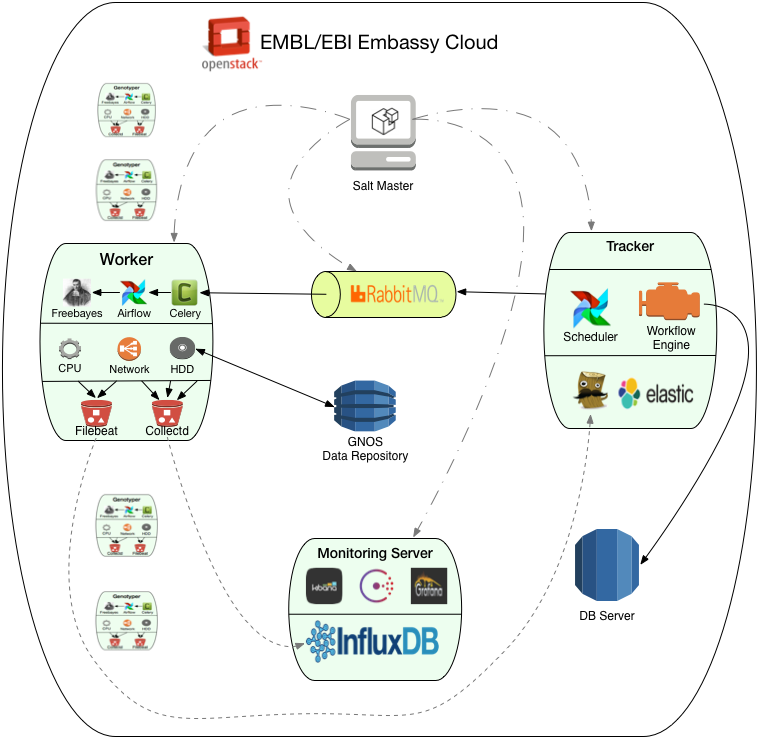
\includegraphics[width=\textwidth]{embassy_butler_deployment_architecture}
\centering
\caption {High level architecture of the Butler framework.}
\label{fig:butler_architecture}
\end{figure}

Butler is different from other popular workflow systems such as Toil\autocite{vivian2017toil}, Nextflow\autocite{di2017nextflow}, or Galaxy\autocite{goecks2010galaxy} because it provides comprehensive functionality in four key areas of concern, while other frameworks typically focus only on workflow execution. These areas are:

\begin{description}
    \item [Provisioning] - Is the set of activities associated with creating, destroying and configuring virtual infrastructure, including network configuration and security. Butler can deploy to virtually any major cloud computing environment and provides helpful tools to make these activities easier.
    \item [Configuration Management] - Is the ability to load and configure arbitrary software package combinations on a variety of platforms. Butler provides ready recipes for the deployment and configuration of any necessary underlying software packages, such as databases, queues, web servers, as well as a wide variety of bioinformatics software. 
    \item [Workflow Management] - Is the system responsible for defining, executing, and monitoring workflows that operate on large data sets. Butler's workflow engine has been tested on clusters with thousands of CPUs, and several ready-made workflows for genomic analysis are available out of the box.
    \item [Operational Management] - Is the set of systems responsible for keeping track of the overall health of the system, including the underlying virtual infrastructure, and any running analyses. There are currently no comparable functionality to Butler's self-healing system in any available scientific workflow software.
\end{description}

We have deployed Butler on a variety of cloud computing environments including OpenStack, Amazon AWS, Microsoft Azure, and Google Compute Engine. We successfully performed large-scale genomic analyses using Butler, and demonstrated their superior performance, as described in the Butler manuscript\autocite{yakneen2017enabling} (in press at Nature Biotechnology).

Three distinct characteristics set Rheos apart from the current generation of genomic analysis frameworks and each of these allows us tackle some of the issues and challenges described above. These are:

\begin{itemize}
\item Service Orientation
\item Event and Data Streaming
\item Random Data Ordering
\end{itemize}

Service orientation\autocite{erl2005service} allows us to decompose the overall problem of comprehensively reasoning about genomic data into a set of small loosely-coupled components, each of which is optimized to tackle a particular well-defined subset of the complete set of requirements of the system. Each service has a contract that it makes with its clients, it has an explicit set of inputs that it knows how to process, it has an interface that defines the modes of communication it supports, it has a set of outputs that it produces according to its capabilities, and it has a set of operational characteristics that makes explicit commitments about the service's reliability, speed, etc\autocite{papazoglou2003service}. This has a number of benefits - a service can be small enough that it optimizes the solution to a particular problem without being subject to the same competing constraints that larger tools are subject to, which provides opportunities for improved performance and hardware utilization. As long as the service respects its input and output commitments it is free to maintain arbitrary internal representations of the data enabling optimization of data storage and query costs ($c_{s}$  and $c_{r}$). A service can be monitored such that hardware is allocated elastically up and down based on demand to ensure optimal utilization, as well as providing a continued measure of whether the service is meeting its operational reliability requirements to its clients\autocite{copil2013multi}. This is especially useful in contexts where demand for certain calculations is highly variable.

The issue of inter-service communication is of major importance because of the large size of the data-set and the potential for various difficult-to-debug run-time race and error conditions inherent in a distributed system\autocite{garcia1984debugging}. Currently, most bioinformatics tools do not communicate with each other directly via an API, instead they use popular file formats such as SAM/BAM/CRAM\autocite{li2009sequence,fritz2011efficient}, and VCF\autocite{danecek2011variant}, as well as a myriad of more esoteric file formats not only as a storage medium but also as a means of communicating information between each other. This paradigm hurts the ultimate scalability of the entire system because of the necessity to write data to disk and possibly move it over the network in order to enable communication across tools. Furthermore, a file-based information exchange mechanism forces a coarse-grained, sample-level, communication between components that wish to avoid tight coupling between each other, even though most of the reasoning about genomic data occurs at locus, or small locus-neighbourhood, levels\autocite{durbin1998biological}. 

Figure \ref{fig:rheos_architecture} shows the high level architecture of the Rheos system. Rheos adopts a data and event stream approach to accomplish scalable fine-grained communication between services\autocite{muthukrishnan2005data}. This approach allows each service to listen to and produce data at the level of granularity that it needs to make decisions, and that its downstream dependencies are interested in (for instance at read, locus, or breakpoint levels). When primary data is ingested into the Rheos system (from a sequencer, or a data repository) the data stream can start to be analysed immediately\autocite{han2011data}, unlike file-based systems that need to wait for the entire sample to transmit before beginning. This approach can potentially enable real-time analysis given sufficient allocation of computational resources\autocite{aggarwal2007data}. Since the raw data is extremely large, it is advantageous to move this data between machines, and between disk and RAM as little as possible, thus instead of passing the raw data around the network various services pass around events of interest about the raw data amongst themselves\autocite{etzion2011event}. When a particular service needs the raw data (rather than the corresponding events) for its decision-making it can be shipped this data as necessary, or it can be instructed to run on the host that has already cached this data in memory. Data streaming allows for extreme scalability, but a key challenge when dealing with data streams is that one is no longer guaranteed to ever be able to see "all of the data" for a particular sample, at least in any meaningful amount of time\autocite{gaber2005mining}. Because genomic algorithms frequently make use of various summary statistics accumulated over the data-set\autocite{patel2012ngs,li2013aligning}, not being able reason over all the data at once means that approximations for these summary statistics are required. Rheos uses approximations calculated within time windows over the data stream\autocite{datar2002maintaining,babcock2002models} and we consider their properties in detail in the body of this thesis.

\begin{figure}[H]
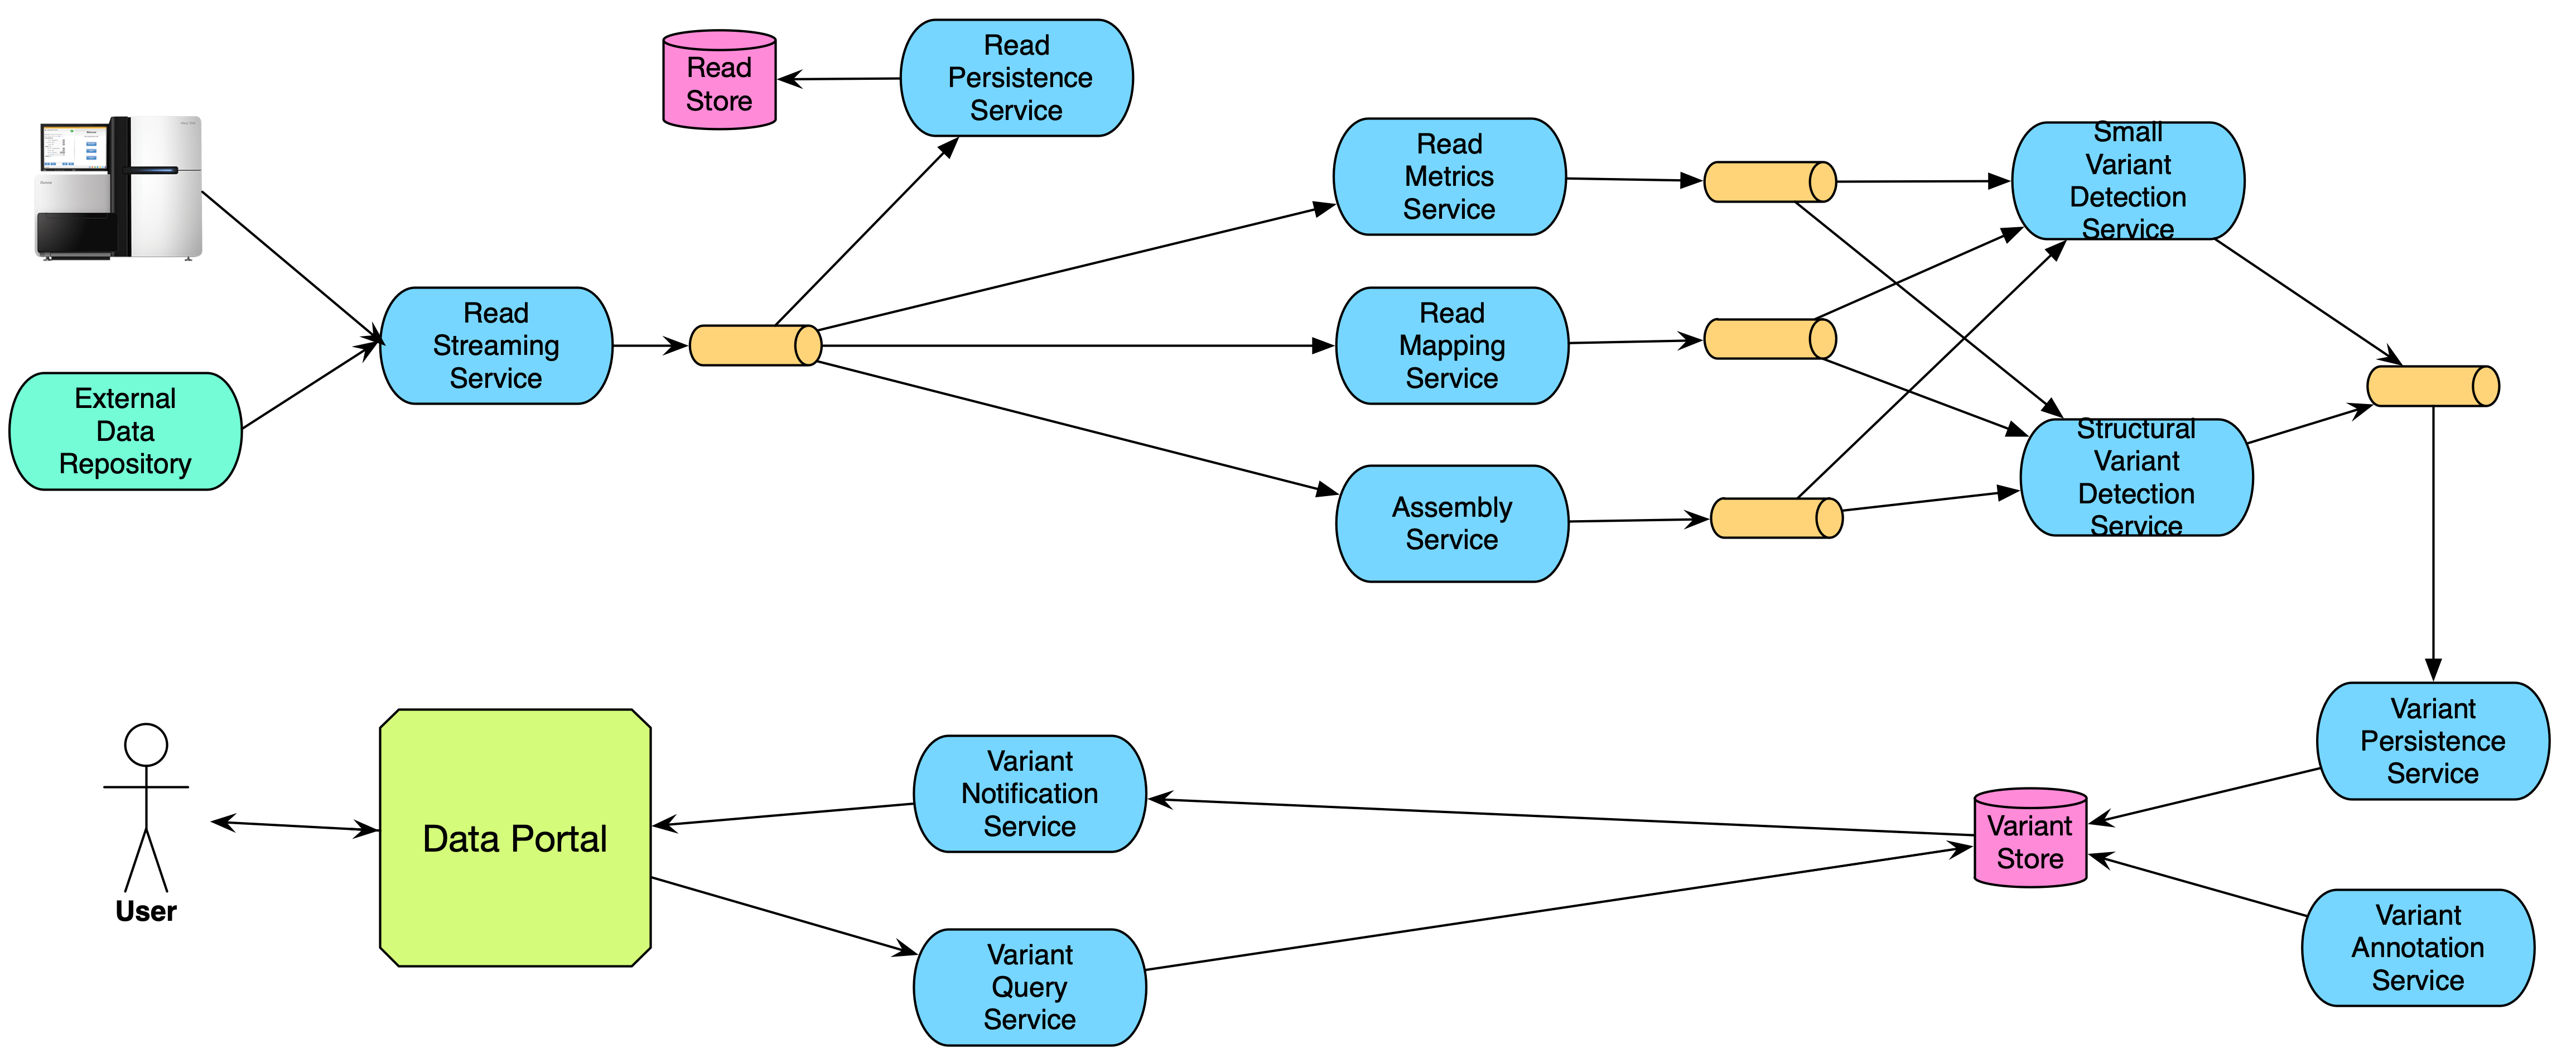
\includegraphics[scale=0.38]{rheos_high_level}
\centering
\caption {High level architecture of the Rheos framework.}
\label{fig:rheos_architecture}
\end{figure}

A key assumption made by nearly all algorithms in the genomics space that participate in variant calling and reason over sequence reads is that the reads are coordinate-sorted with respect to the reference genome to which they are aligned\autocite{li2009sequence,garrison2012haplotype,cibulskis2013sensitive,rimmer2014integrating}. The algorithms then proceed by traversing the genome in coordinate-wise fashion from the beginning of chromosome 1 to the end of chromosome Y interrogating each locus in turn by examining the set of reads that overlap that locus (a read pileup)\autocite{li2009sequence}. Getting the reads into a state that is usable by these algorithms then requires, at a minimum, that all the reads for a given sample have been generated, have gone through QC\autocite{whalley2017framework}, have been aligned\autocite{li2010survey}, have been investigated for PCR duplicates\autocite{van2013fastq}, and have been sorted\autocite{van2013fastq}. Each of these steps can take hours or even days to complete, especially on high coverage whole genome samples. We take a different approach with Rheos by relaxing the requirement for the reads to have been sorted before any variant calling can take place, and instead develop a set of variant calling algorithms that do not assume any particular order within the data that they observe. This allows Rheos to make use of sequence data as soon as it comes off the sequencing machine, thereby dramatically reducing the total time $T$ required to process genomic data compared to the current generation of algorithms. Rheos accomplishes this by employing the service- and stream-based approaches discussed above to process each read on-the-fly as it moves through the system. The read is first assessed for quality, then aligned to a reference genome by the alignment service. This service emits an event with a coordinate that corresponds to the alignment. Variant calling services listen to this event stream and incorporate the evidence for genomic variation supplied by this read into their models of the genomic features that exist at that particular locus for that sample via a statistical framework based on an iterated application of Bayes' rule\autocite{zacks1971theory,berger2013statistical}. 

Because current generation tools can see all of the data for a particular locus at once they can incorporate all of the evidence supplied by this data in a minimal number of calculations, corresponding to each particular algorithm\autocite{li2009sequence,garrison2012haplotype}. Rheos, on the other hand, to incorporate the same amount of evidence will need to perform a larger number of calculations in a redundant manner, incorporating the data as it is observed. This cost is compensated for, however, by the fact that Rheos can immediately incorporate new data about a particular locus when it becomes available without the need to have accumulated all of the data for all of the loci, generating significant time savings. Furthermore, because data arrives in no particular order the set of variant calls produced by Rheos at any given point in time represent a comprehensive characterisation of the sample as if the sample was sequenced at an average coverage consistent with the amount of data that has been observed so far. Observing more data is equivalent to raising the average coverage uniformly throughout the genome, thereby improving call accuracy\autocite{alioto2015comprehensive}. This provides us with a framework to actively and dynamically trade off call-set accuracy $A$ for processing time $T$ and cost $C$ as actual data is being observed thereby enabling novel applications whereby sequencing is abandoned early when issues such as sample-swap\autocite{ewen2000identification}, or contamination\autocite{cibulskis2011contest} are detected. In addition, when sufficient accuracy is reached based on observed data at a particular locus, the framework may choose to stop looking at further data, whereas current generation approaches necessitate committing to a particular sequencing depth a-priori. Furthermore, because current methods iterate through the data in a coordinate-wise manner, their partial results are not really usable until the entire data-set has been traversed (as they represent only a particular region of the genome), whereas Rheos call-sets represent progressive elaboration of a complete genomic characterisation and are thus usable at any level of accuracy that is fit for the purposes of the underlying analysis. We develop the details of the statistical framework used by Rheos and compare its theoretical and real performance to current generation frameworks in the body of this thesis.

We conceived of Rheos as a modern bioinformatics framework that aims to enable the large scale genomics studies of the future\autocite{england2016100,kaiser2016biden,margolis2014national} in both research and clinical contexts by providing a toolset that allows for interpretation and comprehensive characterisation of high coverage human whole genome samples at the scale of millions of samples. In order to meet the diverse requirements of its users the framework allows users to make informed and dynamic tradeoffs along the optimization dimensions of of cost, accuracy, and time. Rheos unique abilities rest upon three characteristics that set it apart from current generation tools, these are: service orientation, data streaming, and random data ordering. Taken together these characteristics enable Rheos to perform at unprecedented levels of scale while retaining call-set accuracy and reducing per-sample processing time. We dedicate the main body of this thesis to the development of the theoretical framework underlying Rheos, exploring its characteristics, benefits and tradeoffs, discussing its implementation, and evaluating and comparing Rheos' performance to the current best practices in genomics algorithms on real data.  

\section{Thesis Outline}
This thesis focuses on the development of the conceptual framework behind the Butler and Rheos platforms, the  properties of the various workflows and algorithms employed by these tools, and the implementation and experimental validation of the frameworks on real data. Chapter \ref{ch:background} provides an introduction to the fields of genomics, including cancer genomics and clinical genomics, a survey of the main tools and algorithms that are commonly used in genomics is provided including the details of the underlying statistical models and operational characteristics. The chapter concludes with a look at workflow frameworks that tie individual algorithms together into computational pipelines. Chapter \ref{ch:butler_architecture} describes the set of requirements necessary for building a large scale scientific workflow framework, and proposes a system architecture the implements these requirements. Chapter \ref{ch:butler_implementation} describes the actual implementation of the Butler framework and provides a detailed analysis of system performance in the context of real projects. Chapter \ref{ch:rheos_framework} sets up and describes the conceptual framework underlying Rheos based on the approaches of Service Orientation, Data Streaming, and Random Data Ordering, mentioned above. We describe the overall architecture (Section \ref{sec:rheos_streaming_architecture}) as well as the model behind individual services that comprise Rheos and investigate the theoretical properties of the algorithms that underlie Rheos-based genomic analysis (Section \ref{sec:rheos_domain_specific_problems}). Section \ref{sec:rheos_implementation} describes the actual implementation of the Rheos framework's components and investigates their operational characteristics. Section \ref{sec:rheos_validation} is dedicated to the experimental evaluation of Rheos in comparison to other extant frameworks and algorithms using real genomic data. We conclude this work in Chapter \ref{ch:conclusion} with a discussion of the results and an examination of the future direction of Butler and Rheos development.




\chapter{Background and Related Work} \label{ch:background}
\section{Genomics}
The field of genomics is closely related to, yet distinct, from the field of genetics, which itself stems from the work of such seminal figures as Charles Darwin\autocite{originofspecies} and Gregor Mendel\autocite{mendel1865}. While genetics largely focuses on the study of single (or relatively small numbers of) genes - the \emph{genotype}, and how genetic variation and mutation affect the physical traits of a given cell or organism - its \emph{phenotype}, genomics focuses on larger scale events and mechanisms that tend to act on the entirety of an organism's genome, shaping its architecture and ultimately affecting its survival.

\subsection{History of Genomics}
Each living cell is a bio-chemical machine that carries out a number of complex behaviours such as interactions with the surrounding environment, motility, metabolism, and reproduction, that are necessary for its survival and proliferation, based on a genetic program that is encoded within the cell's DNA. The DNA is nominally subdivided into functionally distinct areas known as \emph{genes}. The cell utilizes the program within each gene by first \emph{transcribing} the DNA into an intermediary information-carrier molecule called RNA, and then \emph{translating} this RNA into molecules called \emph{proteins} that are utilized by the cell to carry out the majority of its functions. Understanding and interpretation of the underlying genetic program thus underpins our ability to comprehend the entirety of the different behaviours that each cell undertakes.

The success of this undertaking is contingent, first and foremost, on our ability to effectively read off the information encoded in the DNA, an activity known as \emph{sequencing}. We are able to sequence DNA thanks to the pioneering work of researchers Rosalind Franklin\autocite{franklin1953molecular}, James Watson, and Francis Crick\autocite{watson1953molecular} who first elucidated the physical structure of DNA, then followed by the work of Fred Sanger\autocite{sanger1977dna,sanger1975rapid} who devised the first effective DNA sequencing method. The sequencing method allows us to transform information that is physically encoded on the DNA molecule via a sequence of four distinct types of \emph{basepairs} - Adenine, Cytosine, Guanine, and Thymine into a string stored on a computer using a four-letter alphabet - A,C,T, and G, thus turning DNA interpretation into a digital information processing problem.

While the entire length of the DNA of an organism ranges from several hundred thousand basepairs for simple organisms like viruses and bacteria, to about 3,000,000,000 basepairs for a human, to over 150,000,000,000 for certain plants\autocite{pellicer2010largest} the limitations of Sanger DNA sequencing technology are such that the sequencing machine can only produce DNA fragment strings, known as \emph{reads} that are 800 - 1,000 basepairs long\autocite{sanger1977dna}. Reconstituting the original complete DNA sequence from partial overlaps between reads is thus a costly, time consuming, and computationally intensive problem known as \emph{de-novo assembly}\autocite{zerbino2008velvet}. Once one such full sequence (known as a \emph{reference} sequnce) is assembled however, sequencing other individuals of the same (or closely related) species becomes a significantly easier undertaking. Rather than assembling the sequence \emph{de-novo} one can search for a position on the reference sequence that provides the best matching \emph{alignment} between the reference and each read obtained for the specimen under study. This technique is known as \emph{genomic alignment}\autocite{li2009fast} or \emph{mapping} and yields for each fragment a coordinate that represents where on the reference sequence the fragment maps to. Furthermore, because the DNA of any two organisms of the same species is largely identical, with differences occurring at about 0.1\% of all sites (although this depends on DNA mutation rate)\autocite{nachman2001single} researchers are able to significantly reduce the amount of information that is required to fully represent the genome of a specimen by retaining only the information that describes the sites where that specimen is different from the reference sequence for that species. 

A general approach has thus emerged, where each new species of interest undergoes a relatively costly \emph{de-novo} assembly process for the first genome, which then becomes the reference genome for that species. The sequencing of further individuals of that species utilizes, relatively cheaper, \emph{alignment} and identification of \emph{variants} (sites where the individual differs from the reference) to investigate the effect these variants may have on different phenotypes of interest such as disease susceptibility and survival\autocite{manolio2010genomewide}.

Although genomicists study many different types of organisms the study of human genomes garners by far the most attention and research funding\autocite{needcitation} due to the natural desire of humans to better understand ourselves and influence, where possible, genetic factors impacting human longevity and health. Subsequent to the development of DNA sequencing methods by Fred Sanger one of the most audacious and crucial projects for the development of genomics as a branch of science has been The Human Genome Project\autocite{lander2001initial} - an international effort to sequence and \emph{de-novo} assemble the first complete human genome consisting of chromosomes 1-22, X, and Y (as well as mitochondrial DNA) and totalling approximately 3 billion basepairs. The project ran for over 10 years, completing in 2001, and cost more than \$3 billion USD. Although the main project effort was completed using the Sanger sequencing method, a competing version of the human genome was simultaneously published by a commercial company led by JC Venter\autocite{venter2001sequence}, using a new sequencing method called shotgun sequencing\autocite{venter1998shotgun}, a method that formed the basis for a new revolution in sequencing technology, now termed Next Generation Sequencing\autocite{schuster2007next}.

\subsection{Next Generation Sequencing}
The Next Generation Sequencing methodology\autocite{mardis2008next} relies on fragmenting the DNA of a subject into millions of fragments that are between 100-500 basepairs (bp) in length, then sequencing all of the short fragments and aligning all the reads to the reference with the aid of a relatively fast algorithm\autocite{li2010survey}. Because NGS sequencing methods are prone to certain errors and biases\autocite{dohm2008substantial}, it is necessary to sequence enough DNA fragments to overlap (or cover) every location in the genome several times (typically 10-30), in order to build a statistical model that will be able to determine the underlying sequence, known as \emph{genotyping}\autocite{nielsen2011genotype}, with a high degree of confidence. Thus, at present, a single sequenced DNA sample will typically contain 1 billion reads with a file size of ~150GB when compressed.

\begin{figure}[H]
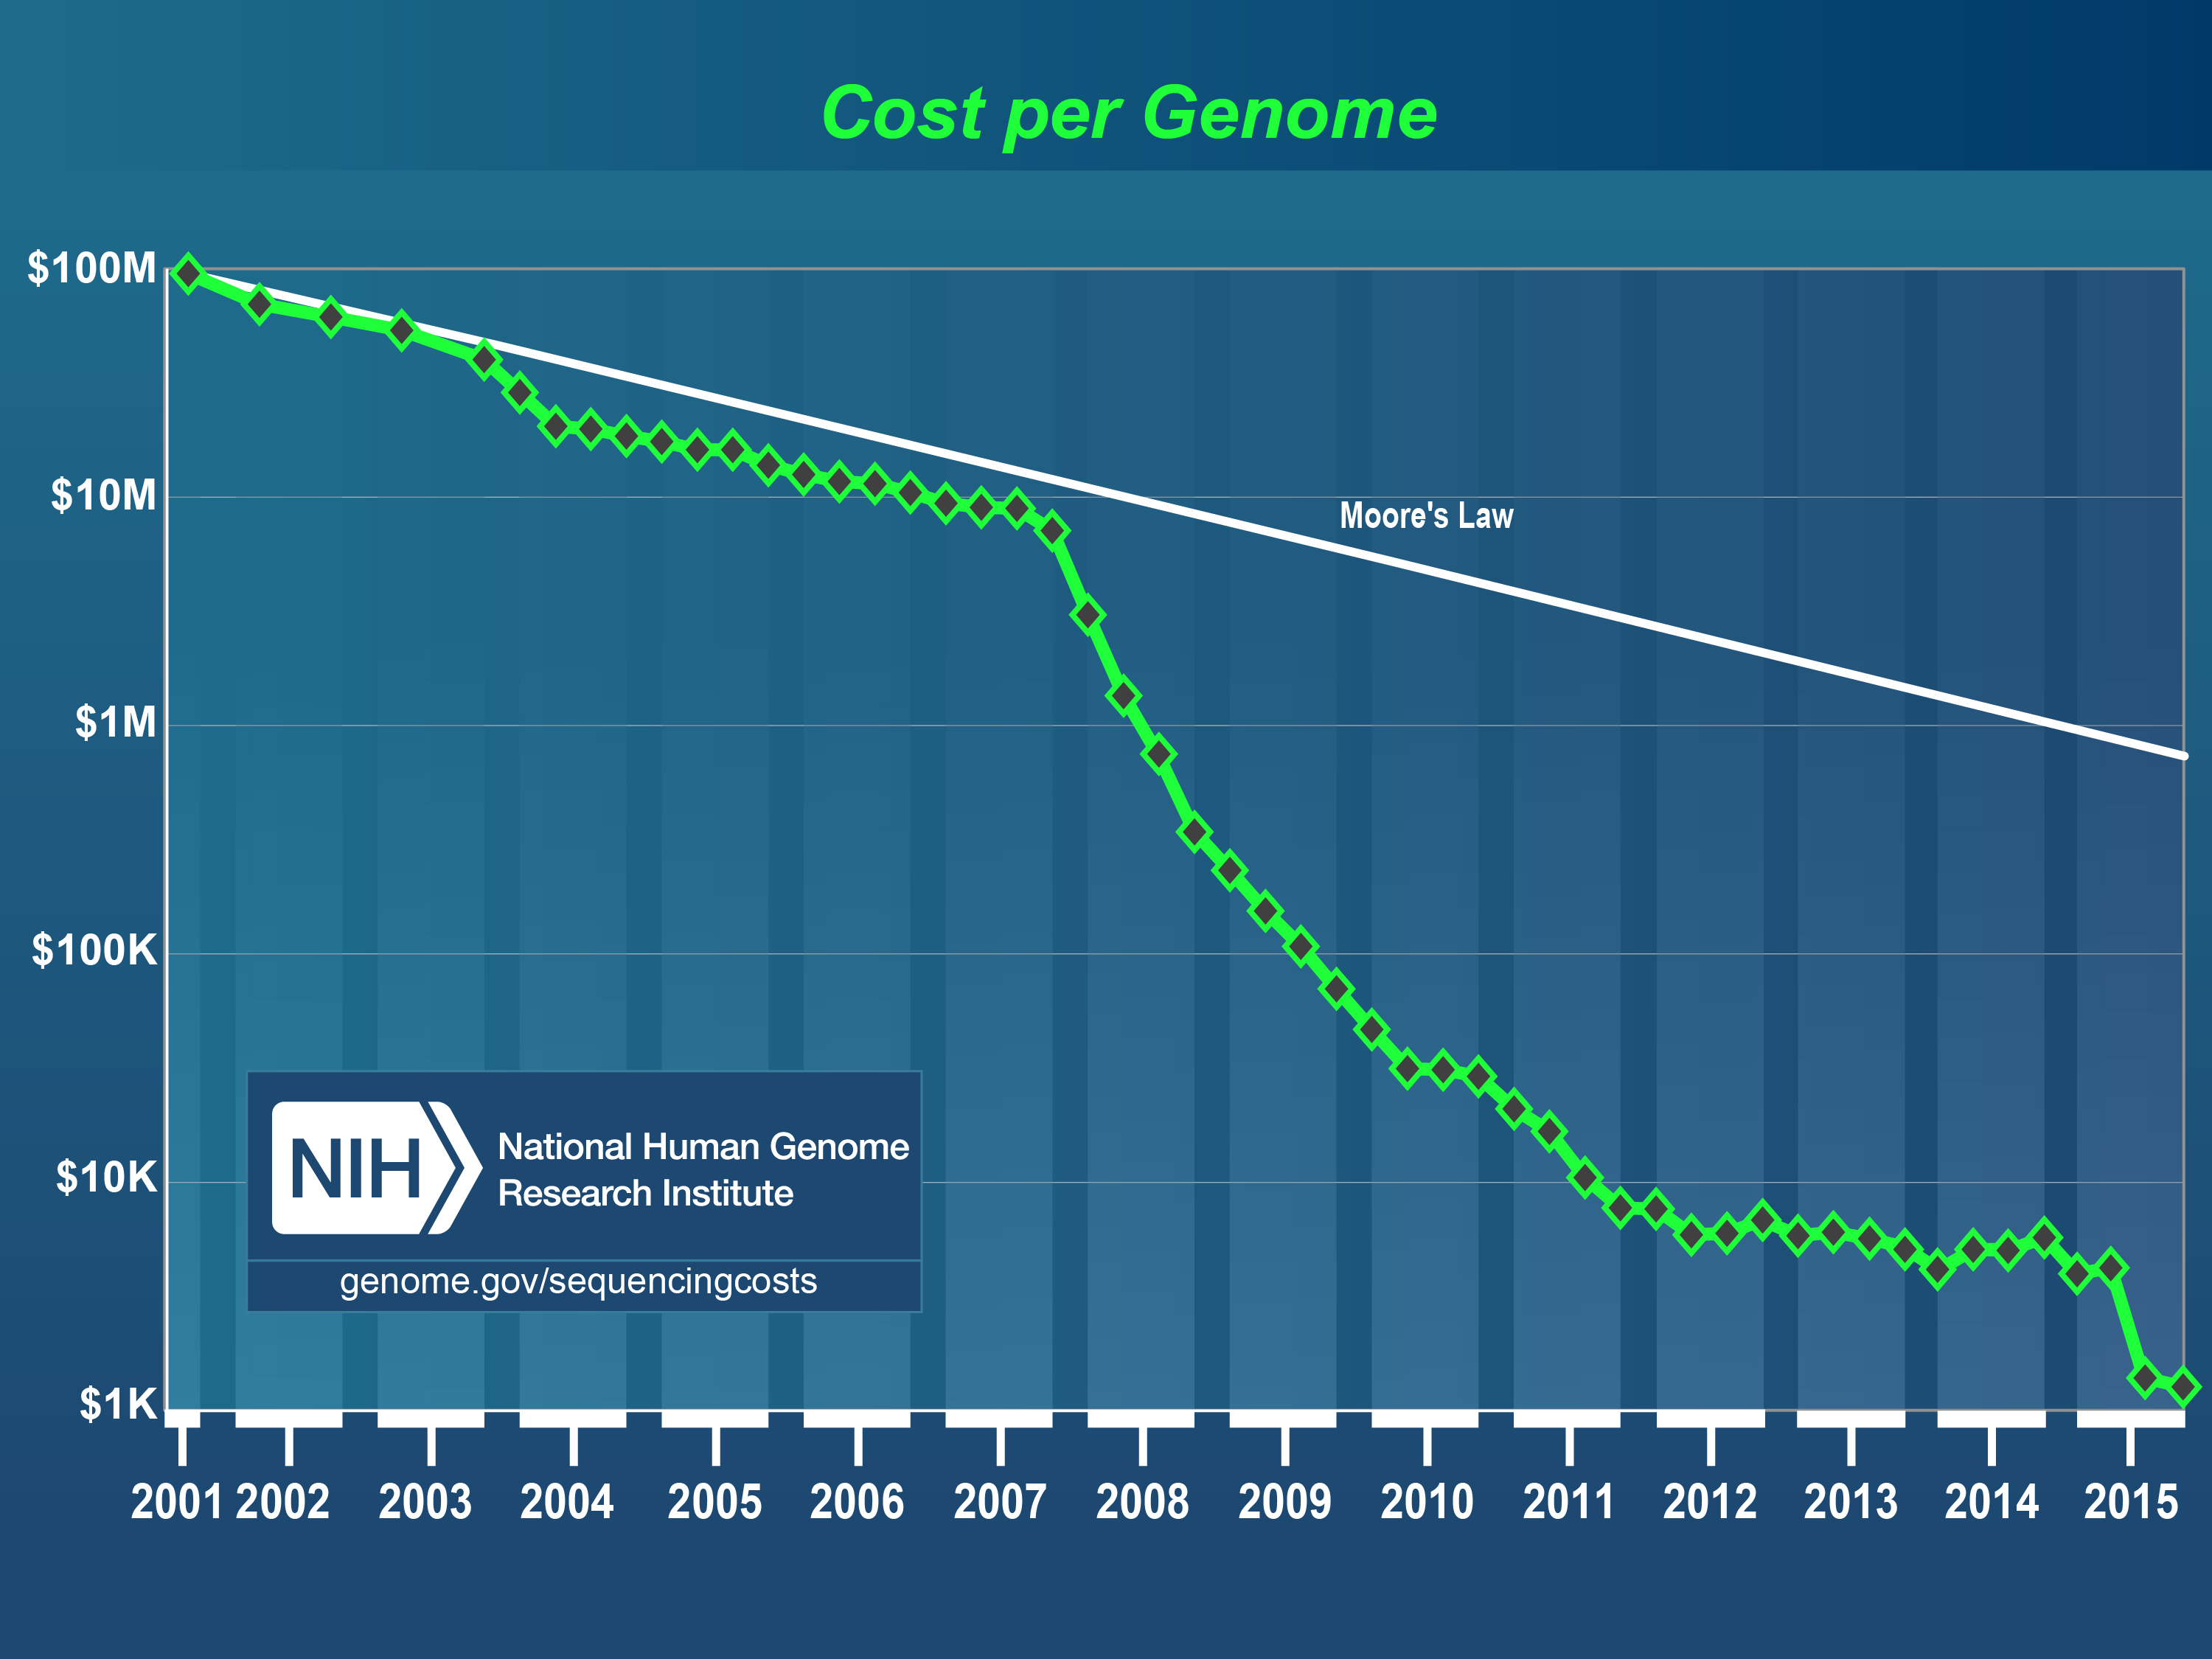
\includegraphics[scale=0.5]{costpergenome2015_4}
\centering
\caption {Cost of DNA sequencing\autocite{The_Cost_of_Sequencing_a_Human_Genome_2016-11-04}}
\label{fig:costpergenome2015_4}
\end{figure}

Figure \ref{fig:costpergenome2015_4} shows the change in the cost of DNA sequencing over the course of the past 15 years. The precipitous drop in sequencing cost observed since 2008 coincides with wide adoption of NGS methodologies. This drop in price has made tractable a new set of large scale genomics sequencing projects that aim to characterize human genetic diversity at population scale, projects such as the 1000 Genomes Project\autocite{10002010map}, and the large scale sequencing of the Icelandic population\autocite{gudbjartsson2015large}.

\subsection{Genomics Studies}

\subsection{Cancer Genomics}
Cancer is a genetic disease that has an extremely high burden on the human population. In 2012, the global incidence of new cases worldwide has been estimated as 14.1 million, and deaths at 8.2 million\autocite{torre2015global}. The economic cost of cancer to the European Union has been estimated at 126 billion euro in 2009\autocite{luengo2013economic}, and in the US \$124.5 billion USD in 2010\autocite{yabroff2011economic}. Because of the genetic nature of the disease studying genomes of cancer patients helps uncover the mechanisms behind the development and evolution of cancer\autocite{stratton2009cancer}.

Cancerous tumours arise from a single cell which over time accumulates a series of somatic mutations that cause it to exhibit properties such as: increased mutation rate, increased proliferation, anchorage independent growth, and resisting cell death\autocite{hanahan2011hallmarks} . Only certain mutations, however, contribute to the development of cancer, while others are benign. Cancer genomics studies aim to identify and characterize those mutations that are cancer drivers and play a role in the formation or progression of tumours\autocite{stratton2009cancer}. 

Studying cancer genomes is more complex and expensive than studying the genomes of healthy individuals because each patient requires that two DNA samples are collected - that of the normal tissue, and that of the tumour. This is necessary to identify those mutations that are somatic - i.e. only occur in the tumour cell population\autocite{roberts2013comparative}.


\begin{figure}[H]
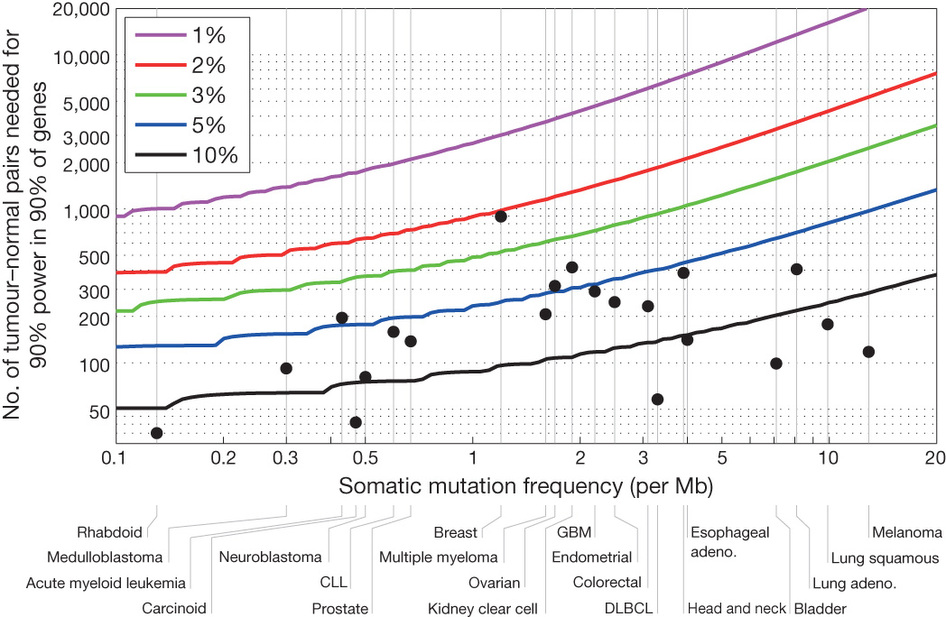
\includegraphics[scale=0.4]{nature12912-f5}
\centering
\caption {Sequencing sample size required by mutation rate\autocite{lawrence2014discovery}.}
\label{fig:nature12912-f5}
\end{figure}

Although there is a large number of identified mutations that are implicated in cancer (2,002,811 SNV,  10,534 gene fusions, 61,299 genome rearrangements, 695,504 CNV segments in COSMIC v70; August 2014)\autocite{forbes2015cosmic}, each mutation has a low chance of being present in any given tumour. Figure \ref{fig:nature12912-f5} demonstrates the sample size required to have 90\% statistical power to identify  90\% of the variants that occur with a set frequency in tumours with varying background mutation rates. Thus, identifying 90\% of the mutations occurring with a frequency of at most 1\% in Lung Adenocarcinoma requires a sample size of at least 10,000 patients. The necessity to sequence large cohorts of patients in order to be able to comprehensively detect  cancer related genomic variants has led to the creation of several large scale cancer sequencing studies.

\subsection{Clinical Genomics}

\section{Computational Methods for Next Generation Sequencing}
Abracadabraca. Because the size of a typical genome is millions to billions of basepairs long, and current DNA sequencing technology frequently generates errors during the sequencing process, requiring multiple samples of each genomic location to be generated, the amount of data required to be examined in order to characterize even a single sample is well beyond the capabilities of any human. Thus, a multitude of computational approaches are required in order to make the task tractable for individual samples as well as cohorts, and entire populations.

The task of comprehensive characterization of genomic data for an individual is typically decomposed into a series of computational steps, each with its own data representation, and typically developed by a separate research group, which are then assembled into computational pipelines and executed by workflow engines on diverse computing environments. Our goal in this section is to enumerate and describe the individual steps and to provide a survey of the key computational tools and data formats that presently form the set of best practices in this rapidly evolving branch of science. Since Rheos is designed to improve upon these best practices we identify in each section the key mathematical and algorithmic ideas that underpin each approach in order to adapt and translate them into the Rheos framework.

The data that is used in virtually all modern genomics studies is generated on a next generation DNA sequencing machine. Several types of sequencers have been developed but the most frequently used ones are made by Illumina. The raw data produced by such a sequencer is a set of image files, where the color of each pixel represents the corresponding nucleotide base in a DNA strand that is being sequenced in each micro-well of a flowcell, representing the sample of interest. The succession of images produced by each cycle of sequencing then results in a set of reads, a collection of randomly ordered DNA fragments that are further analyzed by downstream tools. The first challenge in generating these reads is the accurate interpretation of pixel colors and mapping them to the corresponding nucleotide bases, known as base-calling. Because all of the currently available DNA sequencing methodologies are imperfect at reading the underlying DNA sequence a number of errors is introduced into the process at various stages and special QA software is required in order to detect and assess the location and severity of the errors. A typical output of the QA process is a filtered set of reads where the lowest quality reads have been filtered out and each base within each read is assigned a quality score which represents the best current estimate of the probability that the base has been called incorrectly. The currently most frequently used file format for storing DNA sequence reads along with their read qualities is a text file known as fastq.

Depending on whether the organism under study has previously been sequenced there may already exist a reference sequence for it i.e. a file that for each genomic location describes the most frequently occurring nucleotide for that species at that location. Humans, and many other species of organisms already have reference sequences available. If the reference sequence for the organism under study is available then the next processing step involves searching for the position in the reference sequence that best matches each read that has been generated for the sample under study in the previous step. The coordinate of the best match is then assumed to be the location in the genome where that particular read has originated from. This process is known as genome alignment and it is very resource intensive for species with large genomes such as humans (~3 billion bases) because a typical sequencing effort will generate at least ~1 billion reads for a single sample, and each read needs to be mapped to the reference genome. This problem is made more difficult by the fact that an organism's genome typically has a large proportion of repeated sequence fragments and thus the generated reads do not uniquely align to a single location on the reference. A list of matching positions is generated instead, where each match needs to be scored and the highest scoring match is assumed to be the true origin of the read. Many alignment algorithms exist but the most accurate and fast ones use a two step process of indexing, implemented via hash tables or prefix/suffix tries, to generate a short list of promising match locations, followed by a more exact local alignment that uses dynamic programming to generate a best match. The alignment process is further complicated by the presence of sequencing errors, various genomic variants, and disease state such as cancer, all of which generate significant (and sometimes drastic) differences between the obtained reads and the reference genome, thus necessitating inexact matching approaches. The best algorithms that are currently available have a typical runtime of 24-48 hours on a modern 8-core machine. The most widely adopted standard for storing the alignment data on disk is the SAM\autocite{li2009sequence} (and its binary and indexed counterpart BAM) format developed in the context of the 1000 Genomes Project. In addition to the sequence data and base qualities that are already available in fastq, the SAM format adds a reference coordinate to each read, an overall mapping quality for the read, and whether each position in the read matches the reference sequence, along with other useful metadata. 

When a reference sequence does not exist, or when it is undesirable to use one, genome alignment tools are inapplicable and a different approach, called de-novo assembly, is used. Under this approach each read is broken into smaller subsequences called k-mers (of length k), these k-mers are then used to build a graph structure called a de Bruijn graph. Unique paths through the graph represent possible arrangements of reads that correspond to the underlying sequence and the highest scoring path is chosen as the true sequence. Using the de-novo assembly approach has some advantages over alignment-based methods because it models the structure of the organism's genome directly as it is observed rather than in relation to a reference. This is because no reference is perfect, but instead each reference has its own set of errors that were introduced in its construction. Furthermore, genomic structural variants, which represent large (hundreds to millions of basepairs long) sequences that may be deleted, duplicated, or inverted within a given genome challenge alignment software because of the alignment errors that they introduce and require sophisticated algorithms to later detect, whereas in the de-novo assembly approach these variants are directly modelled as they occur in the underlying sequence and are thus easier to identify. De-novo assembly has its own set of challenges however related to difficulties dealing with repetitive sequences that are found within the genome, as well as the extremely high resource requirements of de-novo assembly algorithms, especially when it comes to memory. The de Bruijn graph is typically built in memory and can be multiple terabytes in size, thus requiring computers with extremely high memory to process. Since, even when using in-memory graph construction the runtime for a single sample is typically several days, it is impractical to move the graph representation to disk without dramatically increasing the algorithm runtime to the point where its duration becomes unreasonable. In practice whole genome de-novo assembly is currently rarely used for processing human genomic data because of the challenges described above. Instead, modern algorithms supplement read alignment with local assembly of particular genomic regions of interest in order to reap some of the benefits offered by assembly-based methods without incurring all of the costs. 

Once the reads have been aligned they are typically sorted by genomic coordinate so that all of the reads that overlap a given coordinate can be examined together at once. This is an expensive sortation step that does not lend itself well to parallelization and takes several hours to complete per sample. Subsequent to the sortation step is another round of data QA which aims to throw out low quality reads that poorly align to the reference. Care must be taken however, because these low quality reads may not only signal underlying data or sequencing issues like sample contamination, or lane-swap, but may also signal the presence of structural variants or integration of retrovirus DNA into the host under study, both of which are of high interest to properly identify. Thus, it is common to split the sample into reads of high quality that are further assessed with one set of algorithms and a set of reads that map with low quality, or fail to map at all, to be assessed with a different set of algorithms.

At this point the data is ready to begin the process of variant calling, that is, identifying the genomic features of the sample that are different from the reference sequence for that organism (i.e. mutations). It is important to distinguish germline variant calling from somatic variant calling at this time. In germline variant calling we are trying to identify the set of variants that have been passed to the individuals under study from their parents and are thus present in every cell of the organism forming the underlying genetic background of that individual where some variants may be neutral to the organism's survival, some may be beneficial, and some may be deleterious. Comprehensively identifying and classifying these is of significant research and clinical interest as they confer susceptibility or resistance to certain disease vectors as well as potential medical remedies and may act as biomarkers to predict disease prognosis or response to treatment within the groups of patients that harbour them.

Somatic mutations are those that each individual cell accumulates over its lifetime and they are of especial interest in the context of cancer where a certain set of mutations accumulated in a particular sequence and over a period of time disrupt the normal cell lifecycle and result in the formation of a malignant tumour. In this context researchers typically sequence both healthy cells (such as those drawn from the patient's blood) and cancerous cells. Mutations are identified in both and the difference between these sets of mutations is then stipulated to be the set of somatic mutations present within that tumour. Just like in the germline case, not all of the somatic mutations contribute to the formation of the cancer and the appropriate identification and classification of those mutations that do (so-called cancer drivers) is an important question of significant clinical and research importance which we consider further below. From a technical standpoint calling somatic variants is significantly more complex than calling germline variants because healthy cells generally conform to the underlying genetic characteristics of the organism, such as the number of chromosomes and ploidy (23 chromosomes, diploid, for humans), whereas in the cancer cells these characteristics can be severely disrupted with entire chromosomes missing or present in amplified copy number, requiring different and more complex statistical models to accurately identify. An additional complexity that is unique to somatic variant calling is the concept of sub-clonal mutations. These are mutations that have been acquired only by some of the cells within a tumour. Since sequencing samples data from a large number of cells within a tumour the reads from which are all pooled together, only a comparatively low number of reads will contain information about sub-clonal mutations, thus making them more difficult to detect, even though such mutations may have a significant impact on the tumour phenotype and thus would be very important to properly identify.

We typically think of three classes of genomic variants that are identified by different methods and oftentimes by separate tools. The simplest to accurately detect, and most frequently occurring are Single Nucleotide Polymorphisms (SNPs), in the germline case, and Single Nucleotide Variants (SNVs), in the somatic case. These are single basepair substitutions where the germline genome differs from the reference sequence by a single letter (for SNPs), or the somatic genome differs from the germline genome by a single letter (for SNVs). SNPs are quite common in humans and occur at the rate of approximately 1 per 1,000 bases on average, or, equivalently, 3 million per individual. Somatic SNVs have a widely varying incidence rate depending on the type of cancer involved with typical rates between (INSERT RATES HERE). For humans, which are diploid (i.e. have two copies of each of the chromosomes, except for the sex chromosomes X and Y), we classify SNPs and SNVs as being either heterozygous (with one reference allele and one variant allele) or homozygous (with both alleles being variant). Methods to detect and accurately genotype SNPs and SNVs typically rely on counting the reads that overlap a given genomic position and evaluating a statistical model that contrasts the probability of the site being reference versus the probability of the site being variant in the face of potential sequencing errors which are expressed as base quality scores and mapping quality scores (as previously described). The models employed for somatic SNV detection and genotyping are significantly more complex than the models for germline variant detection because of the possibility of sub-clonal mutations (as previously described) as well as regions of amplified copy number (i.e. regions where the organism is no longer diploid but can have any number of additional copies of a chromosomal region, or an entire chromosome). More advanced methods output not only lists of variant sites for a sample but calculate a distribution of genotype likelihoods, i.e. all the possible genotypes at a given variant site along with their relative probabilities so that these can be integrated into the models of downstream statistical analyses in a comprehensive manner.

Indels represent sequence insertions and deletions that are anywhere from 1 basepair (bp) to about 50 basepairs long. There is no strict upper bound on the length of an indel and individual tools typically decide on their own cutoffs for length although pretty much all tools place their cutoff at a length that is smaller than the typical read length (150 - 500 bp presently). Indel callers typically look for several mismatched bases in a row between the reference and the sample under study and classify the entire length of the mismatched sequence as an insertion or deletion correspondingly. Other indel callers borrow some of the methodology from structural variant callers which are similar to indels, only typically bigger in size, and are potentially more complex.

Structural variants (SVs) are more large scale genomic rearrangements that occur in both germline and somatic genomes and can have a very drastic effect on the organism's phenotype because they can affect a large number of genes at once, resulting in the loss of function of particular important genes, or the creation of gene fusions where, because of a rearrangement, one gene comes under the programmatic control of another gene thereby disrupting important cellular processes. The most common types of structural variants include insertions, deletions, segmental duplications, inversions, and translocations. Simpler structural variants sometimes combine to produce more complex events that are especially difficult to detect properly. The methods for calling and genotyping of structural variants typically rely on looking at the reads that are deemed low quality for the SNP calling process. These are reads that fail to map to the reference genome, split-reads, which are reads where one part of the read maps to one location on the reference and another part of the read maps to another location, and divergently mapped reads (sequencing is frequently done on read pairs where two ends of a DNA fragment of standard size are sequenced in the opposite directions generating a pair of reads with a standard distance, called insert size, inbetween them), with a shorter or longer than expected insert size. SV callers break down these reads into smaller fragments (k-mers) and attempt to map these k-mers to the reference sequence. The goal is to determine the location of breakpoints, which are positions on the sample genome where a DNA strand break is thought to have occurred as part of the genomic rearrangement that has taken place. Once a list of breakpoints is obtained the algorithm attempts to reconstruct the most likely event sequence that these breakpoints could have arisen from, pairing up adjacent breakpoints that are the result of a sequence deletion, for example. Thus, each pair of breakpoints typically gives rise to a single SV call in the final output of the caller. SV calling is a complex and error-prone process that generates double-digit false-positive and false-negative rate, especially in the somatic case, where patient genomes can undergo drastic rearrangements as a result of cancer-related processes such as chromothripsis and are thus extremely difficult to resolve with accuracy.

Once variants (SNPs/SNVs, Indels, and SVs) have been comprehensively called, a filtering step is necessary because callers are typically initially tuned for highest sensitivity in order to detect the most variants, thus admitting an increased number of false positive calls. Additionally, because calling of SNPs and SVs typically occurs separately by different tools there can be significant call-set overlap where the SNP caller sees a region as a group of SNPs, whereas the SV caller will see it as a single breakpoint. These overlaps need to be resolved in order to avoid redundant calls. A number of filtering approaches exist, some of which rely on heuristics such as strand bias, or read support to filter out low quality variants. Other filtering approaches rely on curated variant databases or machine learning methods in order to reduce the number of false positive calls. One popular filtering approach involves ensemble calling where several different variant calling methods are used on the same dataset and a variant is excluded unless it is called by multiple tools. These methods are typically able to reduce the false positive rate of the call-set by 5-10\% while only nominally affecting the false negative rate.

When a filtered high quality call-set has been prepared it is of interest to determine which of the variants are likely to have an effect on the organism's phenotype and which variants are likely to have no consequence. This is accomplished via variant annotation. The annotation process consults a database of known genes and other genomic elements (promoters, enhancers, etc.) to determine the likely consequence of each variant based on the type of mutation that it represents i.e. a synonymous mutation (that doesn't change the underlying amino acid) is likely to have no phenotypic effect, whereas a stop gain mutation inside the coding region of a known gene may indicate a potential loss of function of that gene and may thus have a considerable effect on the observed phenotype. When annotating somatic mutations it is important to consider known cancer genes and delineate whether mutations are "passengers" or "drivers" depending on whether they are thought to be driving the carcinogenesis process by constitutively activating a cancer gene or deactivating a tumour suppressor, or they are simply acquired as part of the genomic instability that is induced by carcinogenesis. An outcome of the variant annotation process then, is a list of somatic or germline variants accompanied by a designation of the known genomic features that they fall in, along with an assigned functional impact. This is typically the last step of an NGS analysis pipeline after which the variant call-set is considered completed and can be used for any number of downstream analyses depending on the particular research question or clinical application being considered. For instance, the variants may be used as input into a Genome Wide Association Study (GWAS), a Quantitative Trait Locus (QTL) analysis, a rare variant association study, or as input into the computation of a clinical biomarker. 

\subsection{File Formats}
FASTQ - 
BAM/SAM -
CRAM -
VCF - 

\subsection{Base-calling}

\subsection{Alignment}
BWA/MEM -
Bowtie - 
Gem - 

\subsection{Raw Data QA}

\subsection{Germline SNP Calling}

Single Nucleotide Polymorphisms or SNPs are locations in an individual's genome where that individual differs from the reference sequence at a single position. The reference sequence is haploid i.e. it provides a single base (for instance T) at every genomic location, whereas the human genome is diploid (there are two copies of each chromosome, and thus two bases at each location) for chromosomes 1-22, and chromosome X for females, while being haploid for chromosomes X and Y for males. Thus, at each genomic location, the human genome may be:

\begin{description}
    \item [Homozygous Reference] - When both alleles carried by the individual at that location match the reference.
    \item [Heterozygous] - When one allele matches the reference and one is different from the reference.
    \item [Homozygous Alternate] - When both alleles are the same and different from the reference.
    \item [Multiallelic] - When both alleles are different from the reference and are different from each other\autocite{hodgkinson2010human}.
\end{description}

SNPs are the most common type of genomic variant, with every individual carrying over 3 million SNPs on average\autocite{shen2013comprehensive}. Furthermore, the presence of certain SNPs is strongly associated with disease\autocite{wellcome2007genome}, where some SNPs are known to be causative\autocite{ingram1957gene}, while others, are merely associated with a disease phenotype\autocite{satake2009genome}. A large number of scientific studies\autocite{hirschhorn2005genome} and clinical practice\autocite{yang2013clinical} is thus enabled by efficient and comprehensive characterization of the gamut of human SNPs to assess their contribution to disease risk, see Figure \ref{fig:genetic_architecture_of_cancer_risk}.

\begin{figure}[H]
    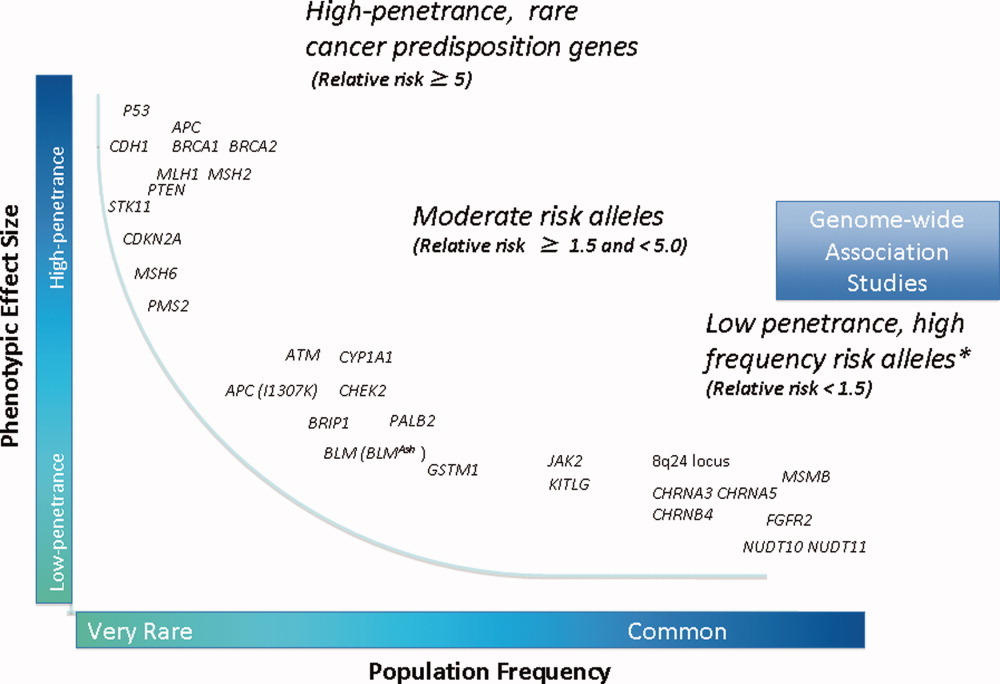
\includegraphics[scale=0.55]{genetic_architecture_of_cancer_risk}
    \centering
    \caption {Distribution of mutations by population frequency against phenotypic effect size.\autocite{weitzel2011genetics}.}
    \label{fig:genetic_architecture_of_cancer_risk}
\end{figure}

There are a number of methods that have been used for assessing SNPs with the aid of microarry technology\autocite{heller2002dna}, but here we focus on methods that make use of Next Generation Sequencing (NGS). Since the primary data type generated by NGS is a sequencing read, most presently used methods for SNP detection rely on investigating the collection of sequencing reads that overlap each genomic locus and comparing the observed data to the reference sequence. It is important to distinguish two typically separate activities that take place as part of SNP calling - variant calling, and genotyping. Variant calling attempts to locate positions in the sample genome where that sample is different from the reference, whereas genotyping attempts to assign an actual genotype (e.g. homozygous-alternate), along with a measure of confidence, to each putative variant. We present several of the key computational methods currently used in SNP calling with additional detail. These are:

\begin{itemize}
    \item samtools
    \item freebayes
    \item GATK
    \item platypus
\end{itemize}

These tools have been selected because they have been developed independently, at different institutions, and have been repeatedly demonstrated to produce consistent and high-quality results. See Figure \ref{fig:fb_hc_st_pt} for a recent comparison.

\begin{figure}[H]
    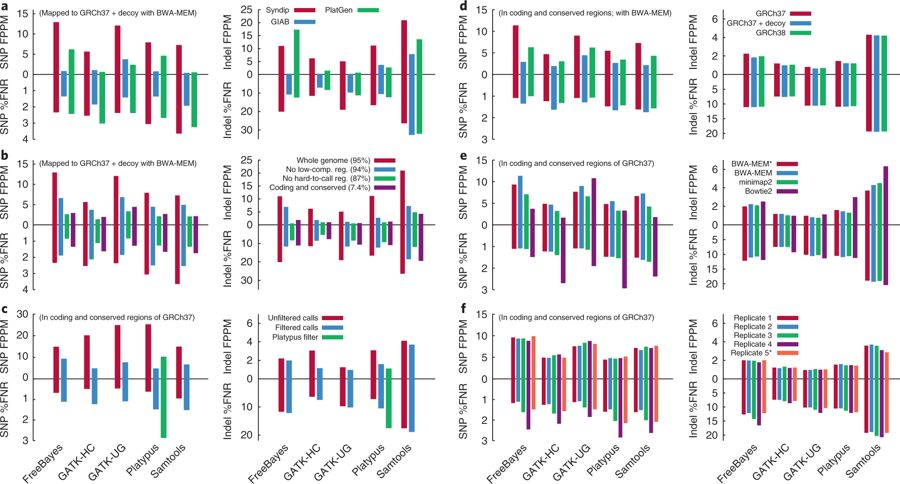
\includegraphics[scale=0.45]{fb_hc_st_pt}
    \centering
    \caption {Comparison of samtools,freebayes, GATK, and platypus on three benchmark data sets - Syndip, GIAB, and PlatGen. Here FPPM - number of false positives per megabase of sequence, and FNR - false negative rate = 100xFN/(TP+FN).\autocite{li2018synthetic}.}
    \label{fig:fb_hc_st_pt}
\end{figure}

\subsubsection{samtools}
Samtools\autocite{li2009sequence} is a software package for genomic data processing developed by Heng Li et al. in the context of the 1000 Genomes Project\autocite{10002010map} and implemented as a C program with a CLI interface. This tool has enjoyed continued and widespread use in the bioinformatics community for the purposes of small variant calling (including SNPs). All of the mathematical results in this section are reproduced from the 2011 paper by Li\autocite{li2011statistical} that describes the method, as well as a set of mathematical notes made available separately by Li\autocite{li2010mathematical} in 2010.

Although the samtools framework could be extended to support calling multi-allelic sites, the framework, as-published, has been developed for calling only bi-allelic variants. Table \ref{tab:samtools_notation} contains commonly used definitions.

\begin{table}[!htb]
    \caption{Samtools common notations}
    \label{tab:samtools_notation}
    {\begin{tabular}{lp{7cm}}
    \toprule
    Symbol & Description \\
    \midrule
    $n$ & Number of samples \\
    $m_i$ & Ploidy of the $i$-th sample ($1\le i\le n$)\\
    $M$ & Total number of chromosomes in samples: $M=\sum_i m_i$\\
    $d_i$ & Sequencing data (bases and qualities) for the $i$-th sample\\
    $g_i$ & Genotype (the number of reference alleles) of the $i$-th sample \mbox{($0\le g_i\le m_i$)}$^1$\\
    $\phi_k$ & Probability of observing $k$ reference alleles ($\sum_{k=0}^M\phi_k=1$) \\
    $P(A)$ & Probability of an event $A$\\
    $\mathcal{L}_i(\theta)$ & Likelihood function for the $i$-th sample: $\mathcal{L}_i(\theta)=P(d_i|\theta)$ \\
    \bottomrule
    \end{tabular}}
\end{table}

It is additionally assumed that there are $n$ individuals being sequenced with the $i$-th individual having ploidy $m_i$ (typically 2 in practice). At a particular genomic locus, the sequence read data for the $i$-th individual is $d_i$ and the genotype is $g_i$, an integer in $[0,m_i]$, counting the number of reference alleles in the individual at that locus. Furthermore, it is assumed for simplicity that data at individual genomic loci are independent (which isn't necessarily true), as are sequencing and mapping errors between loci and individuals.

Because of the above independence assumptions the joint likelihood function of the data observed for all individuals factors as a product of individual likelihood functions:

\begin{equation}
    \mathcal{L}(\theta)=\prod_{i=1}^n\mathcal{L}_i(\theta)
\end{equation}

Suppose that a single sample $i$ represents an individual of ploidy $m_i$ and a given locus is covered by $k$ reads. The sequencing data $d_i$ is composed of an array of bases where each element has value 1 representing the reference allele and is 0 otherwise. 

\[
d_i=(b_1,\dots,b_k)=(\underbrace{1,\ldots,1}_l,\underbrace{0,\ldots,0}_{k-l})
\]


The error probability of the $j$-th base is $\epsilon_j$, which is taken to be the larger between sequencing and mapping errors for that read. Under the independence assumptions above:

\begin{equation}
    \mathcal{L}_i(0) = P(d_i|0)=\prod_{j=1}^l\epsilon_j\prod_{j=l+1}^k(1-\epsilon_j)=\left(1-\sum_{j=l+1}^k\epsilon_j+o(\epsilon^2)\right)\prod_{j=1}^l\epsilon_j
\end{equation}
\begin{equation}
    \mathcal{L}_i(m_i) = P(d_i|m_i)=\left(1-\sum_{j=1}^l\epsilon_j+o(\epsilon^2)\right)\prod_{j=l+1}^k\epsilon_j
\end{equation}
For $0<g_i<m_i$:
\begin{eqnarray}\label{eq:gd}
    \mathcal{L}_i(g_i) = P(d_i|g_i)&=&\sum_{a_1=0}^1\cdots\sum_{a_k=0}^1\Pr\{d_i|B_1=a_1,\ldots,B_k=a_k\}\Pr\{B_1=a_1,\ldots,B_k=a_k|g\}\\\nonumber
    &=&\sum_{\vec{a}}\left(\frac{g}{m}\right)^{\sum_j a_j}\left(1-\frac{g}{m}\right)^{k-\sum_j a_j}\cdot\prod_j p_j(a_j)\\\nonumber
    &=&\left(1-\frac{g}{m}\right)^k\prod_j\sum_{a=0}^1 p_j(a)\left(\frac{g}{m-g}\right)^a\\\nonumber
    &=&\left(1-\frac{g}{m}\right)^k\prod_{j=1}^l\left(\epsilon_j+\frac{g}{m-g}(1-\epsilon_j)\right)\prod_{j=l+1}^k\left(1-\epsilon_j+\frac{\epsilon_jg}{m-g}\right)\\\nonumber
    &=&\left(1-\frac{g}{m}\right)^k\left\{\left(\frac{g}{m-g}\right)^l+\left(1-\frac{g}{m-g}\right)\left(\sum_{j=1}^l\epsilon_j-\sum_{j=l+1}^k\epsilon_j\right)+o(\epsilon^2)\right\}
\end{eqnarray}
where $a=\sum_j a_j$ and
$$
p_j(a)=\left\{\begin{array}{ll}
\epsilon_j & \mbox{$a=1$}\\
1-\epsilon_j & \mbox{$a=0$}\\
\end{array}\right.
$$

In particular, for a diploid sample ($m=2$), the likelihoods for $g=0,1,2$ are
\begin{eqnarray*}
\mathcal{L}(0)&=&\prod_{j=1}^l\epsilon_j\prod_{j=l+1}^k(1-\epsilon_j)\\
\mathcal{L}(1)&=&\frac{1}{2^k}\\
\mathcal{L}(2)&=&\prod_{j=1}^l(1-\epsilon_j)\prod_{j=l+1}^k\epsilon_j\\
\end{eqnarray*}

For instance, taking $g_i = 2$ (i.e. the true genotype is homozygous-reference) as an example, and under above independence assumptions, the likelihood of observing the data $d_i$ is the likelihood of sampling $l$ reads without error (the reads match the reference) and $k-l$ reads with error (the reads do not match the reference).

Given that $\phi$ is some prior distribution of genotypes (a model from population genetics can be used, or an empirical distribution from antoher study), the actual genotype for individual $i$ at the given locus is estimated via Bayes' Rule as:

$$
\hat{g}_i=\argmax_{g_i} \Pr\{G_i=g_i|d_i,\phi\}=\argmax_{g_i}\frac{P(d_i|g_i)P(g_i|\phi)}{\sum_{h_i}P(d_i|h_i)P(h_i|\phi)}
$$

\subsection{Germline Indel Calling}

\subsection{Germline Structural Variant Calling}
Delly - 
Hydra - 

   s
\subsection{Variant Filtering}

\subsection{Somatic SNP Calling}
Mutect - 
Muse - 
Pindel -


\subsection{Somatic Indel Calling}

\subsection{Somatic Structural Variant Calling}

\subsection{Germline Variant Annotation}
Annovar - 
Variant Effect Predictor - 


\subsection{Somatic Variant Annotation}

\subsection{de-novo Assembly}
Velvet -
Abyss - 

\section{High Performance and High Throughput Computing}

The practice of performing large scale scientific computation on supercomputers or clusters of commodity hardware can be split into two notions - High Performance Computing (HPC) and High Throughput Computing (HTC).

The European Grid Infrastructure defines these as follows\autocite{Glossary_V1_-_EGIWiki_2016-10-28}:

\fbox{\parbox[c]{0.9\textwidth}{HPC - A computing paradigm that focuses on the efficient execution of compute intensive, tightly-coupled tasks. Given the high parallel communication requirements, the tasks are typically executed on low latency interconnects which makes it possible to share data very rapidly between a large numbers of processors working on the same problem. HPC systems are delivered through low latency clusters and supercomputers and are typically optimised to maximise the number of operations per seconds. The typical metrics are FLOPS, tasks/s, I/O rates.}}

\fbox{\parbox[c]{0.9\textwidth}{HTC - A computing paradigm that focuses on the efficient execution of a large number of loosely-coupled tasks. Given the minimal parallel communication requirements, the tasks can be executed on clusters or physically distributed resources using grid technologies. HTC systems are typically optimised to maximise the throughput over a long period of time and a typical metric is jobs per month or year.}}

Although early High Performance Computing efforts (1960's - 1980's) relied on supercomputers with a shared memory model\autocite{russell1978cray}, where all of the memory was shared between multiple processors, by the late 1980's machines with a distributed memory model\autocite{nitzberg1991distributed}, where each processor has its own memory, started gaining ground, forming the basis for the modern HPC cluster.

The software interface that the user has to a HPC/HTC cluster typically takes the shape of a queueing system such as PBS\autocite{henderson1995job} or LSF\autocite{zhou1992lsf}  where the user writes a script that submits a series of jobs to the queueing system. The jobs can invoke software that is installed by the IT department that manages the cluster. The user is not able to install any software and has limited visibility into the runtime performance characteristics of the jobs they submit. 

\section{Cloud Computing}

Cloud computing has emerged in the early 2000's enabled by improvements in hardware virtualization which was driven by the adoption of Virtual Private Networks, and the desire to commercialize access to compute capacity as a utility\autocite{buyya2009cloud}.

The National Institute of Standards and Technology provides a standard definition of cloud computing that encompasses several areas of this domain - Essential Characteristics, Service Models, and Deployment Models\autocite{mell2011nist}.

The Essential Characteristics of a cloud are as follows:

\begin{description}
\item [On-demand self-service] - End-user can independently manage infrastructure without involving the service provider.
\item [Broad network access] - Cloud resources are available on the network via a set of standard protocols.
\item [Resource pooling] - Service providers dynamically assign virtual infrastructure in a multi-tenant environment based on consumer demand.
\item [Rapid elasticity] - Resources can be elastically provisioned and discarded according to customer requirements.
\item [Measured service] - Resource usage by end users is measured and transparently provided back to the user by the service provider.
\end{description}

It is the self-service and broad network access characteristics that set cloud computing apart from traditional HPC computing the most.

Service Models include:

\begin{description}
\item [Infrastructure as a Service (IaaS)] - This service allows the the user to provision and control virtualized infrastructure such as VMs and networks.
\item [Platform as a Service (PaaS)] - This service allows the user to deploy their application onto virtualized hardware but not to control the management of the infrastructure.
\item [Software as a Service (SaaS)] - This service allows the user to make use of applications that are deployed on virtualized hardware but not to manage the applications or the infrastructure itself.
\end{description}

The Deployment Models covered by the NIST definition are as follows:

\begin{description}
\item [Private Cloud] - Operated privately by a single organization and not accessible on a public network.
\item [Community Cloud] - Established for use by a particular community of users with a common interest.
\item [Public Cloud] - Established for general use by the public.
\item [Hybrid Cloud] - A collection of cloud entities that use one of the other deployment models but allow application portability.
\end{description}

The first publicly available commercial cloud computing platform has been developed by Amazon.com and launched in August, 2006 in the form of two services - Elastic Compute Cloud (EC2), and Simple Storage Service (S3). Cloud offerings by Microsoft and Google followed in 2010, and 2012. This early lead has allowed Amazon to capture the majority of the public cloud computing market, earning \$2.57 billion USD in Q1 2016 revenue.

One of the main drawbacks, however, of using Amazon's or another proprietary cloud solution is the issue of "vendor lock-in" i.e. inability to easily switch infrastructure providers should the customer wish to do so, because of the amount of software relying on the proprietary cloud provider protocols. Another key reason for avoiding public clouds is the necessity to store sensitive data. This issue applies both to the commercial enterprise (with industries such as banking, and payments) and scientific domains (especially genomics and medicine) where handling of sensitive patient data is restricted based on both technical security, as well as ethical considerations\autocite{knoppers2005human}.

To help alleviate these concerns an open-source cloud platform called Openstack was launched in 2010 jointly by Rackspace Hosting and NASA\autocite{sefraoui2012openstack}. Openstack provides most of the same features that are provided by Amazon Web Services and other commercial cloud providers as free open-source tools. These include:

\begin{itemize}
\item Infrastructure
\item Networking
\item Identity Management
\item Block Storage
\item Object Storage
\item Managed Databases
\item Queues
\item Monitoring
\end{itemize}

Openstack deployments for the basis for most academic private and community clouds such as EBI Embassy Cloud\autocite{cook2016european}, University of Chicago Open Science Data Cloud\autocite{grossman2010overview}, Cancer Genome Collaboratory\autocite{yung2016icgc}, and Helix Nebula\autocite{marx2013biology}. Because these clouds implement the security measures necessary when handling patient data they are a system of choice for large scale bioinformatics analyses.

\section{Workflow Systems}

The focus on workflow stems the work of Frederick Taylor (1856-1915) and Henry Gantt (1861-1919) on the improvement and automation of industrial processes, also known as "scientific management"\autocite{taylor2004scientific}. One of the key techniques that were devised at the time and served as the prototype for future workflows were "time and motion studies"\autocite{barnes1949motion} where employees were observed as they performed repetitive cycles of work in order to determine standard execution times and sequences of steps. As this field evolved over the course of the 20th century it gave rise to several other related fields such as Operations Management, Business Process Management, and Lean Manufacturing.

In 1993 an international consortium was formed with the purpose of defining the standards related to workflows and workflow management systems. This consortium is called the Workflow Management Coalition (WfMC). One of the key specifications produced by the WMC in 1995 is The Workflow Reference Model\autocite{hollingsworth1995workflow}. This document provides two basic definitions that illuminate the scope and purpose of  workflow systems:

\fbox{\parbox[c]{0.9\textwidth}{Workflow - The computerised facilitation or automation of a business process, in whole or part.}}

\fbox{\parbox[c]{0.9\textwidth}{Workflow Management System - A system that completely defines, manages and executes "workflows" through the execution of software whose order of execution is driven by a computer representation of the workflow logic.}}

A number of standards have been produced for workflow definition, many of them are XML-based\autocite{shapiro2002technical}. Notable examples include:

\begin{description}
\item[XPDL] - Was developed by the WfMC, currently at version 2.2, as of 2012. Uses an XML dialect to express process definitions
\item[BPML] - Developed by the Object Management Group (OMG) using XML. Deprecated as of 2008 in favour of BPEL.
\item[BPEL/BPEL4WS] -  Developed by Organization for the Advancement of Structure Information Standard (OASIS). Uses XML format. Adopted by Microsoft and IBM for their workflow products - 
\end{description} 

Graphically, workflow definitions are typically expressed using a Petri-Net\autocite{peterson1981petri} or Business Process Model and Notation (BPMN), the latter borrowing its structure from UML activity diagrams. A set of workflow definition design patterns exists to guide workflow creation\autocite{van2003workflow}. A workflow engine is responsible for ingesting workflow definitions, generating their graphical representation, and allowing the user to execute the workflow definitions on suitable hardware.

As initially the focus of workflow systems research and development has been on process improvement within commercial enterprises there exists a large pool of workflow engine implementations targeted at that sector. Some of these are:

\begin{description}
\item[jBPM] - An open-source workflow engine that is based on the Java platform and is currently owned by Red Hat.
\item[Activiti] - An open-source workflow engine that has been developed by previous jBPM developers.
\item[Oracle BPEL Process Manager] - A commercial workflow engine acquired by Oracle from Collaxa in 2004, now integrated into the rest of the Oracle portfolio.
\item[Websphere Process Server] - Commercial workflow engine that is part of IBM's Business Process Manager suite.
\end{description}

Although these tools have gained wide adoption in the enterprise community they have had limited success within scientific circles. Instead, several open-source workflow management systems exist that have been purpose-built for the scientific domain, and especially bioinformatics. These include:

\begin{description}
\item[Kepler\autocite{ludascher2006scientific}] - A Java-based WfMS built on top of the Ptolemy II\autocite{davis1999overview} execution engine.
\item[Taverna\autocite{oinn2004taverna}] - A Java-based WfMS originally built by myGrid, currently under incubation at Apache Software Foundation. 
\item[Galaxy\autocite{goecks2010galaxy}] - A Python-based WfMS developed specifically for bioinformatics applications with a focus on GUI-driven development of workflows.
\end{description}

Curcin et al\autocite{curcin2008scientific} provide a head-to-head comparison of six scientific workflow systems including Taverna and Kepler, whereby Taverna is described as primarily being aimed at researchers who wish to build scientific workflows from web services utilizing a proprietary XML dialect called SCUFL which implements a DAG model of workflows. The primary execution environment for a Taverna workflow is on a grid or an HPC cluster. Kepler implemented a different methodology, whereby workflow modelling, which is taken on by Actors, is separated from workflow execution, taken on by Directors. An Actor knows only about its inputs, the computation that it needs to perform, and the output that it needs to produce, while Directors provide different models of execution, such as Synchronous Data Flow, Process Network, Continuous Time, and Discrete Event.

The Galaxy workflow framework has a specific focus on bioinformatics analyses and comes with a large library of community-developed bioinformatics workflows. The user creates and executes workflows via a web-based GUI where pre-installed tools and scripts can be laid out into a pipeline. The primary deployment environment for Galaxy is on an institutional HPC cluster although a separate component allows the deployment of a Galaxy instance on Amazon Web Services\autocite{afgan2010galaxy}.

\section{Service Oriented Architectures}

\section{Stream-based Systems}


	 
\chapter{The Butler Framework - Requirements and Architecture} \label{ch:butler_architecture}
%In this chapter we specify a set of requirements for a large-scale cloud-based scientific workflow framework. The chapter is split into two sections - Section \ref{sec:functional_requirements} Functional Requirements deals with requirements for how to access data, install software, manage workflows, and troubleshoot errors, Section \ref{sec:non_functional_requirements} Non-functional Requirements deals with issues of Scalability, Availability, Ease-of-use, and Interoperability.

\section{Functional Requirements}\label{sec:functional_requirements}

Running scientific analyses requires the following broad set of capabilities:
\begin{itemize}
\item Access to data
\item Access to compute capacity
\item Implementations of one or more scientific algorithms
\item A workflow that defines the sequence of steps in the analysis
\item A workflow engine that handles job scheduling and execution
\item A system of record for what analyses have been performed
\item A set of tools for troubleshooting error conditions
\end{itemize}

Operating such a system on the cloud necessitates an extra set of capabilities that enable users to take advantage of the scalability and elasticity offered by cloud computing, while retaining cost effectiveness and security. These capabilities include:
\begin{itemize}
\item Provisioning of cloud infrastructure
\item Configuration of virtualized hardware
\item Service discovery
\end{itemize}

\subsection {Access to Data} \label{sec:access_to_data}

Scientific analysis typically requires access to data files to run various tools on, thus an analysis system needs to provide a mechanism for accessing data. Depending on the architecture of the system in question, several data sources can be identified, each of which stipulates a particular data access mechanism. These include:

\begin{itemize}
\item Data stored in a third party data repository on the internet
\item Data stored on a network accessible shared storage folder
\item Data stored on cloud specific Block Volumes (such as Amazon's EBS, or Openstack Cinder)
\item Data stored on cloud specific Object Storage Services\autocite{factor2005object} (such as Amazon S3, or Google Cloud Storage)
\end{itemize}

\subsubsection{3rd Party Repository Data}

Bioinformatics, like many fields of science, has a vast number of data repositories and reference data sets available over the Internet, in both, free access, and authenticated modes. The method of access to these services is typically specific to each repository, although is frequently limited to HTTP and FTP protocols. Thus, a cloud-based system that allows access to external IP ranges via HTTP and FTP should be able to meet this requirement to a sufficient degree.

\subsubsection{Network Accessible Shared Storage}

A large data repository that is hosted within the same data center as the compute cluster is the data access method of choice within HPC deployments, but is also used within cloud computing environments, especially private academic clouds. A distributed network accessible file-system such as Isilon OneFS, Lustre, GlusterFS, MooseFS, GFS, or HDFS is typically used\autocite{sawant2013big}.  In order to take advantage of such a shared file-system a cloud-based compute cluster simply needs to have mount privileges on the cluster virtual machines. Once mounted, the file-system can be accessed as if it was a local file-system. It is typically the case that full root is available on cloud-based VMs, so this method of access remains both popular and well supported, especially for analyses where multiple VMs may need to access the same file at the same time. 

This approach has three key drawbacks:

\begin{itemize}
\item Shared access to a file server can run into scalability bottlenecks at the storage and network layers as the number of VMs simultaneously accessing the resources increases. High performance storage providers such as Netapp and Isilon can support simultaneous transfer rates of up to 40 GB/s, which allows a significant number of VMs to simultaneously access the shared resources, however, as shown in the Experimental Validation section, even 1000 compute cores can easily consume over 25\% of that bandwidth, thus limiting the overall system scalability to about 4000 cores.
\item While academic cloud providers are frequently running a large scale shared storage server in support of their HPC environments, commercial cloud providers do not have this service out of the box, thus it is up to the user/operator to set up such a shared file-system based on VMs and block-storage volumes (and possibly ephemeral disks), which can be a significant cost.
\item Implementing data access security is challenging, because once a shared file-system is mounted, data access is granted based on Unix groups without checking credential validity with the data owner.
\end{itemize}

\subsubsection{Block-level storage}

Most clouds provide a block storage service (Amazon, Google, Microsoft, Openstack, and others). Block storage is different from typical hard-drives that are available as a standard together with Virtual Machines, in that the standard hard-drives are considered "ephemeral" storage - their contents are available only for the lifetime of the VM that they are attached to. Due to the short lifetime, such storage is typically only acceptable for use as scratch-space, and not for the long-term storage of data under analysis. Block storage volumes offer an alternative, whereby a block storage device can be attached and detached to any VM within the same data center without the loss of information. Once attached, the block storage volume can be mounted as if it was normal local storage. 

For the purpose of scientific analysis on the cloud, block-storage offers an attractive option whereby a data set can be prepared and staged on a block storage volume outside the scope of a particular analysis, and can then be mounted on a VM that will perform the analysis, as well as being reusable for other analyses downstream. 

Key drawbacks of this approach are:

\begin{itemize}
\item The same block volume cannot be mounted by several VMs at once, thus causing data duplication, or ruling out this data access method, where simultaneous access to a file by several VMs is required.
\item Limited size of a single block storage volume (currently 16TB on Amazon for instance).
\item Higher storage cost than object storage.
\end{itemize}

Block level storage is automatically available in all cloud environments where such a service is present and it is up to individual analyses to take advantage of this method of data access. 

\subsubsection{Object Storage}

Most cloud products on the market today provide an object storage service. Examples of this are Amazon S3, Openstack Swift, Ceph\autocite{weil2006ceph}, and Microsoft Blob storage.  Object storage provides a highly scalable alternative to shared filesystems and block storage volumes, where each object of interest is stored in a "bucket" and can be retrieved by its identifier.  This method of access is especially attractive because data access security can be implemented on an individual object basis, something that is difficult to implement with other data access methods. Thus, scientific analyses that operate on sensitive data, such as those performed for the biomedical field with human subjects can greatly benefit from adopting this method of access for cloud-based analysis. Additional benefits of object storage include virtually limitless scalability of storage space, and low cost, relative to other storage methods.  

A drawback of this approach is that object storage based systems do not function in the manner of POSIX compliant file systems that many are familiar with. Thus, an analysis framework that wants to support object storage as a method of data access needs to provide support for managing user credentials, retrieving data of interest by identifier from the object storage and into a scratch space available to the VM (such as ephemeral disk or block storage volume), writing intermediate analysis results back to the scratch disk, and storing the final analysis results back into object storage based on a predetermined bucket structure.

\subsection {Access to Compute Capacity} \label{sec:access_to_compute_capacity}
Running analyses requires access to computational resources such as CPU and RAM and doing so on the cloud is significantly different from the way the same goal is accomplished in traditional HPC environments.

A traditional HPC environment has a static pool of resources, access to which is facilitated via a queueing system. All users submit their jobs to a priority queue and each job is eventually scheduled to run on some server. The server is a long running machine, which is not dismantled between jobs, and the user has little control over the server's configuration in terms of software or hardware. If the HPC data center operates in a cost-sharing model, costs are apportioned based on either a fixed allocation between departments or research groups, or based on resources used during the job execution.

Because access to cloud-based resources is charged based on time-in-use i.e. by the hour, or by the minute, running analyses on the cloud requires a different mode of operation in order to remain cost effective. Virtual Machines need to be created from scratch and used only for the duration of time strictly required by the analysis, at which point they need to be destroyed. Furthermore, because the cost of each Virtual Machine is directly related to the amount and type of resources that it consumes, and the user has complete control over this configuration, it is in the user's interest to optimize the hardware configuration of each VM such that it fits the type of analysis being performed as some analyses will benefit from higher CPU, RAM, optimized disk I/O, etc. A successful framework for cloud-based analysis then needs to provide the following capabilities in the area of Access to Compute Capacity:
\begin{itemize}
\item Ability to authenticate and interact with multiple cloud-provider APIs
\item Ability to define hardware configurations of Virtual Machines.
\item Ability to easily create and destroy Virtual Machines based on pre-defined hardware profiles.
\item Ability to specify network topology and security rules.
\end{itemize}

\subsubsection{Interact With Multiple Cloud-Provider APIs}
Because there are many cloud providers out there, each with certain advantages and disadvantages when it comes to features and cost it would be beneficial for a generic analysis framework to be able to interact with as many cloud provider APIs as possible. This is challenging because different cloud APIs are in-general incompatible although similar in nature, and it is necessary to provide a translation layer, so that the users of the framework do not have to learn different API dialects depending on which environment they wish to deploy to. Authentication methods typically rely on a known URL, username/password, and a public/private key pair, and thus are fairly amenable to standardization.

\subsubsection{Define Hardware Configurations for VMs}
Because each type of analysis may require several flavours of VMs, each with a different hardware configuration, it would be beneficial for the user if the analysis framework provided a mechanism to easily define such configurations in a human readable file that can be versioned and source controlled. Key fields that need to be captured by such a configuration file include:

\begin{itemize}
\item VM naming template
\item Number of VMs
\item Number of CPUs
\item Amount of RAM
\item Number and type of hard disks
\item Security Groups
\item SSH Keys for logon
\item Initial machine image or snapshot to use (to avoid starting from a completely empty VM)
\item Network configuration (IP address, subnet, floating IP)
\item Post-initialization commands (such as registering with a master node or updating packages)
\end{itemize}

\subsubsection{Create and Destroy Virtual Machines}
Due to the dynamic nature of cloud computing clusters where Virtual Machines are frequently created and destroyed it is necessary to provide a convenient method for carrying out both of these operations on a large number of VM instances and in a cloud agnostic manner. The user should be easily able to dispose of any number of running machine instances by name, as well as being able to create any number of new machines based on the templates described in the previous section

\subsubsection{Define Network Topology and Security Rules}
While in an HPC system the network topology and security are completely specified by the IT group, it is up to the user to adequately specify both in a cloud computing environment. Thus, a user needs to be able to specify networks, traffic routing rules, and control access to resources within the network based on port, protocol, and address of the requester. This requirement is especially important when it comes to handling and managing human genomic data which is highly confidential - a typical network and security configuration that needs to be supported is one where a central network router controls access to and within the cloud tenant. Only a limited number of known IP addresses from the internet are allowed inbound access over a secured protocol. Furthermore, Virtual Machines within the cluster are completely locked down except for a limited number of ports and protocols, as necessitated by their role within the cluster.

Because cloud computing clusters are frequently created and torn down it is necessary to be able to express the network and security configuration as a set of rules that can be easily re-instantiated as needed.

\subsection {Implementations of Scientific Algorithms} \label{sec:algorithm_implementation}
Running scientific algorithms en-masse is the key requirement for a scientific workflow management system, and even though the implementation of the algorithms themselves is outside of the scope of such a framework, existing algorithm implementations need to be easily brought into the system and configured for running.  In an HPC environment tool installation is performed by the IT department managing the HPC cluster, but in a cloud computing environment it falls upon the user to carry out installation of all software, thus a system of support is required for managing installations of scientific software on Virtual Machines in the cloud.

Several mechanisms for installing software on VMs exist and need to be supported:
\begin{itemize}
\item Installation of a binary file from a known URL
\item Compilation of a tool from source code
\item Installation of a Virtual Machine image
\item Installation of a lightweight container image
\end{itemize}

\subsubsection{Installation of a Binary File}
Oftentimes tool authors provide compiled versions of their software on the Internet. These are typically available for major operating systems. If such a tool does not have other dependencies, then installing it simply requires access to a particular URL on the Internet from the VM that the tool needs to be installed on. From a security perspective this means allowing outgoing traffic from VMs inside the cluster for protocols such as HTTP, HTTPS, FTP, SFTP, FTPS and their associated ports. Installation then proceeds by retrieving the required binary resource and possibly setting up some symlinks for convenient invocation.

\subsubsection{Compiling From Source Code}
A large proportion of scientific software exists as source code available over the Internet on sites like Github, Bitbucket, Sourceforge, etc. along with instructions for compiling the software on a supported platform. This provides a major avenue for installation of scientific software and requires capabilities for downloading the source code from the internet via a tool like git, along with possible dependencies, and then executing a build script provided by the tool author, thus requiring the same capabilities as specified for installing binary files, as well as possibly elevated user privileges for installing services or adding users.

\subsubsection{Installation of a VM Image}
Several widely used formats of VM Image exist, such as OVA, OVF, VMDK, AMI, etc. A tool author may choose to make their algorithm available as a complete VM image that can be instantiated within a cloud computing cluster. This is especially true for complex applications that have many dependencies and very specific OS requirements that are hard to replicate reliably. The process of instantiating VM images is typically similar between cloud providers although differences exist.

\subsubsection{Installation of a Lightweight Container}
A more lightweight approach than using entire VM images is shipping software via a lightweight container such as Docker\autocite{merkel2014docker}. This method of software distribution is gaining in popularity in the last two years. Lightweight container images are typically smaller than entire VM images as they only concern themselves with providing an application runtime environment, rather than an entire VM emulation, and they typically allow the running of multiple such containers simultaneously on a single VM in a micro-services container-based architecture. 

In order to support this method of distribution the cloud computing cluster needs to be running a container management platform such as Docker Swarm or Google Kubernetes.

\subsection {Workflow Definitions} \label{sec:workflow_definitions}
A typical scientific analysis consists of a series of steps where a set of input files (or samples) are transformed through, possibly multiple, computational stages to produce a set of output files that may be used as is, or retained for further analysis. 

\begin{figure}[h]
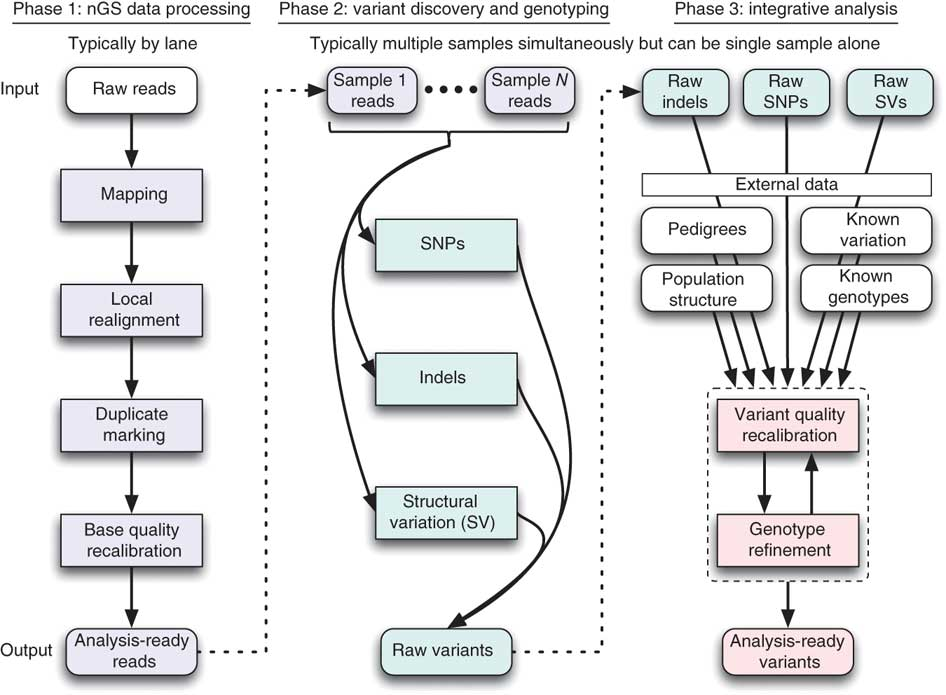
\includegraphics[width=\textwidth]{ng.806-F1.jpg}
\centering
\caption {NGS Workflow\autocite{depristo2011framework}.}
\label{fig:ng.806-F1.jpg}
\end{figure}


To be able to reliably carry out such analyses it is desirable for a system to have a number of capabilities that define the "workflow" of execution steps. These are:

\begin{itemize}
\item Define a structure that encodes a sequence of steps and the conditions for moving from one step to the next.
\item Ensure deterministic behaviour where possible i.e. same inputs produce the same output when run multiple times (whether in the same computational environment or different environments).
\item Ensure that the analysis has a finite run-time where possible.
\item Allow fine-grained control over the analysis configuration. 
\end{itemize}

\subsubsection{Workflow Structure Definition}
An effective and commonly utilized method of representing a workflow in the scientific analysis and other contexts is as a directed graph. Each vertex in the graph represents a particular computational step that needs to be carried out, and graph edges represent, possibly conditional, transitions between the vertices. This representational method allows the user to comprehensively express both the steps involved in an analysis, as well as specifying their sequence and executing control flow. Furthermore, the graph-based approach allows for a graphical representation of the workflow structure that is readily comprehensible by humans, thus increasing its utility. In general, the following requirements need to be met in order for the graph-based workflow representation to be fit-for-use in the scientific analysis context:

\begin{itemize}
\item The workflow should be encoded using a language and format that is easily readable by humans.
\item It should be possible to pass parameters to a workflow -- values that can be used at runtime to affect workflow behavior.
\item A workflow state should be able to invoke any program that is installed on the machine that is running that workflow state.
\item A workflow state should be able to interrogate the environment that it is running on i.e. check for presence/absence of certain files, communicate with a database, access URLs on the Internet.
\item Any number of transitions should be able to enter or leave a state.
\item It should be possible to render a graphical representation of the workflow as an image.
\item It should be possible for different states in a workflow to exchange information.
\end{itemize}

\subsubsection{Deterministic Behaviour}
Scientific reproducibility is a key concern that needs to be maintained in order for the system to be usable in the context of scientific analysis. Reproducibility, specifically, refers to the requirement for a user to be able to produce the exact same result as reported by another user using the same workflow definition, input files, and computing environment. While certain algorithms that may be executed as part of a workflow state like Expectation Maximization\autocite{moon1996expectation}, or Stochastic Gradient Descent\autocite{bottou2010large} behave in a non-deterministic manner where exact reproducibility of results may not be possible, the workflow system itself should not introduce any stochastic components when encoding workflow structure.

\subsubsection{Finite Run-Time}
The directed graph structure allows for transitions back to a previously visited vertex, thus creating graph cycles. Although this improves the expressiveness of the structure it is generally undesirable in the context of workflows as such a workflow may end up in a perpetual loop within the cycle requiring human intervention to diagnose and rectify at run-time. Although it is generally impossible to guarantee a finite run-time for a workflow due to the possibility of any underlying computational algorithm itself getting stuck in a perpetual loop or resource deadlock, we would like to rule out such a possibility at least from the perspective of workflow structure. Thus, we place an additional constraint on the workflow definition to be a Directed Acyclic Graph (DAG). Although this complicates somewhat the encoding of use cases where certain tasks need to repeated a number of times, these use cases are generally still attainable via programmatic generation of a series of states or using sub-graphs and gives us the added comfort of ruling out infinite loops where possible.

\subsubsection{Analysis Configuration}
A scientific analysis typically needs to be configured and parameterized at multiple levels. When considering different types of parameterization required, 3 distinct levels of parameterization can be identified. These are:

\begin{description}
\item[Workflow level] -- configuration that applies to a particular workflow regardless of which analysis it is used on. This may include things like paths to the location of certain programs used by the workflow, or their general invocation strings, or certain reference values.
\item[Analysis level] -- this includes values that may be different from one analysis to the next but are not different between samples under the same analysis.  Examples of such configurations are: common flags to pass to tool invocations, where to store analysis results, where to look up reference data sets.
\item[Execution level] -- these parameters differ even from one invocation of a given workflow under the same analysis to the next invocation. The most common instance of such a parameter is the set of names of input files that need to be processed by the workflow representing one sample. 
\end{description}

It is natural to view these configuration levels as a three level hierarchy where Analysis configurations expand on and override Workflow level configurations, and Execution level configurations expand on and override Analysis level configurations.

In order to successfully configure the workflow system it is necessary to be able to specify and permanently store such configurations in a format that is both human- and machine-readable. Thus, a user who is conceiving a particular analysis should be able to author a set of configurations that embody the nature and specifics of the analysis being performed. These configurations should then be easily transferrable to another individual or system instance for reproducibility purposes. Once the configuration of the system is fully specified the user should be able to launch their analysis according to this specification.

At run-time, the workflow system should be able reconstruct one \emph{effective} configuration from all levels of the configuration hierarchy and apply it appropriately.

\subsection {Workflow Engine} \label{sec:workflow_engine}

A Workflow Engine is necessary for the set of workflow definitions to be executable on a compute cluster. This workflow engine needs to be able to fulfill the following broad set of requirements:

\begin{itemize}
\item Workflow parsing and translation
\item Workflow state management
\item Workflow scheduling
\item Workflow execution
\end{itemize}

\subsubsection{Workflow Parsing and Translation}

While a workflow itself encodes the structure and sequence of computational steps that need to be performed, the workflow engine needs to be able to parse such a workflow definition and translate it into a set of commands that can be runnable on a real machine. To aid scalability it is desirable for the workflow to be broken down into a set of tasks at this stage that can be run on different physical machines. The workflow engine then needs to be responsible for producing this set of uncoupled commands from a monolithic workflow definition.

\subsubsection{Workflow State Management}

Workflow state management encompasses concerns of how to keep track of workflow definitions, including their versioning, as well as the status of various workflow instances. The workflow engine, then, needs to keep a registry of workflow definitions where, along with the workflow code and an identifier, the user can record useful metadata related to that workflow, such as - workflow version, author, owner, creation date, whether the workflow is enabled, etc. This registry is the authoritative source of information on what workflow capabilities a particular deployment of the workflow system has, and every new workflow, or update to an existing workflow must be recorded within this registry.

Furthermore, a particular version of a workflow definition may give rise to any number of workflow instances i.e. particular invocations of the workflow on a set of inputs and within the context of an analysis. Each instance may be in one of a number of different states, such as - Stopped, Running, Queued, Completed, or Failed. The workflow engine is responsible for keeping track of all of the workflow instances for a given workflow, and their states, and is responsible for transitioning the workflow instances from one state to the next, based on the preconditions for each such transition. These state transitions are not to be confused with the state transitions that are encoded within the workflow definition, as the workflow definition state transitions are custom to each workflow and encode the logic of the underlying scientific analysis, whereas the workflow instance state transitions and their conditions are standard for all workflows and workflow instances and describe the general workflow lifecycle. As with the metadata  recorded for workflow definitions, the workflow engine should also record metadata associated with workflow instance state transitions, the most important of which is the time-stamping of all such transitions. 
   
\subsubsection {Workflow Scheduling}

Once a workflow definition is parsed and translated into a series of runnable tasks, the workflow engine needs to be able to schedule these tasks for execution as appropriate. A Scheduler component within the engine needs to be able to match up two sources of information - availability of computational resources, and availability of runnable tasks, to produce a schedule i.e. a set of task-to-resource assignments within an appropriate timeframe. In order to accomplish this the Scheduler needs to be able to carry out a number of tasks, as detailed below.

To ascertain availability of computational resources the Scheduler needs to be able to communicate with all machines within the cloud computing cluster that are designated for running tasks. Furthermore, the scheduler needs to be able to interrogate the state of these machines to determine what the current level of load on each machine is, and whether the machine can accept more load in the form of new tasks. As the load level of each machine is of a dynamic nature, and is based on the completion of currently running tasks, the Scheduler needs to be in a constant state of communication with the entire compute cluster, in order to maintain an up-to-date picture of resource availability.

To establish a list of runnable tasks the Scheduler needs to iterate over all currently running workflows and determine the state of execution within them. As tasks are completed within each workflow instance, other tasks that are downstream from them in the workflow definition may become runnable. The scheduler should then determine for each workflow instance what its set of currently runnable tasks is, based on the structure of each workflow definition and the current state of the workflow instance.

One important concern within the realm of workflow scheduling is the concept of workflow and task priority. It is natural to think that not all workflows, and not all workflow tasks have the same priority i.e. some are more important than others and should, thus, have precedence when it comes to scheduling. It is then important for the Scheduler to be able to incorporate the concept of priority into the task scheduling decisions that it is making in order to meet user requirements.

Armed with a prioritized list of runnable tasks and a list of available resources the Scheduler needs to produce as set of task-to-resource assignments that can be used for workflow execution.

\subsubsection {Workflow Execution} 

The purpose of a workflow engine, at its core, is to execute workflows, thus, a set of execution capabilities is required. The sections above describe the requirements for parsing and translating a workflow into a set of runnable tasks, managing their state, and scheduling task execution according to its priority and resource requirements. The Execution component of a workflow engine needs to handle the actual running of tasks that have been scheduled.

Each machine in the cloud computing cluster that is part of the workflow system needs to be able to accept from the workflow scheduler a task execution assignment that encodes the details of the actual task that needs to be run. The task itself may consist of any number of computational steps. The Execution component is then responsible for transitioning a task from the Scheduled state to a Completed or Failed state, and carrying out the computational steps encoded within the task definition. This typically involves running other programs, collecting their return statuses, and execution timestamps and relaying this information to the Workflow State Management component.

When the Execution component encounters errors during task runtime it should be able to not only collect comprehensive information about the error condition, but should also be able to retry running the task without necessarily failing the overall workflow instance.
   
\subsection {System of Record} \label{sec:system_of_record}

One of the key requirements for a workflow system to be used in a scientific context is reproducibility. This concept was referenced earlier when describing the desire for a workflow to behave deterministically where possible. Another important factor that affects reproducibility is the method by which the course of a scientific analysis is encoded. We thus need an accurate system of record that keeps track of the following information:

\begin{itemize}
\item The various analyses that are undertaken
\item Workflows that are executed as part of each analysis
\item Samples that are part of the analysis
\item Overall system configuration
\end{itemize}

For each of the items above it is important to capture and permanently store a number of vital fields such as names, and unique identifiers, owner, version, and timestamp. Then, when the results of such an analysis are used in a scientific publication it is enough to provide the unique identifier of this analysis to be able to recover the technical details that will aid in reproducing analysis results by a 3rd party.

\subsection {Troubleshooting Errors} \label{sec:troubleshooting}

One of the inevitabilities of large scale computing is the occurrence of error conditions. The probability of an error being encountered in a unit of time increases together with the complexity of an analysis being performed and the amount of computational resources being utilized. In a traditional HPC-based scientific computing centre responsibilities for detecting and handling errors are divided between the end user who is responsible for errors that occur in their data or algorithms, as well as their encoding of cluster compute jobs, and the cluster IT personnel who are responsible for any errors that are caused by the overall software and hardware infrastructure failures. 

Although, it appears as if this division of responsibilities favours the end user by relieving them of the need to handle infrastructure issues, it has a notable downside. The underlying infrastructure and run-time environment are opaque to the end user who is only free to submit compute jobs and collect their results. On the other hand, the majority of errors (of any kind) manifest themselves as compute job failures and it is up to the end user to discern which of these are problems of their algorithm and which are problems of the infrastructure. Because of the opacity of the runtime environment, the end user has few tools at their disposal to be able to accomplish this task effectively and can spend significant effort troubleshooting issues that are outside of their domain of responsibility before being able to hand the incident resolution over to IT.

By contrast, in a cloud computing environment the end user has ownership of the health of the entire virtualized system including the infrastructure and the workloads that are running on it. This alleviates the issue of environment opacity described above but places a slew of new requirements on the operator of such a system when it comes to management of error conditions. Methods for detection and handling of errors differ depending on the source of the errors and we describe these in further detail below.

In general the following sources of error are identifiable and require appropriate handling:

\begin{itemize}
\item Errors within underlying scientific algorithms or the data they operate on
\item Errors within the workflow definition
\item Errors within the workflow engine
\item Errors within the virtual infrastructure
\item Errors within the bare metal hardware/software infrastructure and virtualization layers
\end{itemize}

\subsubsection {Errors Within Algorithms or Data}

Most scientific software is experimental by its nature and is developed by relatively few individuals compared to industry software, thus it is reasonable to expect that error conditions should occur within such software with a higher frequency than within mature and stable enterprise software. There are two standard mechanisms by which a program can return error conditions (whether they arise due to an error within the program or bad data) -- return value, and log files. Both of these should be collected to have the most accurate representation of the state of running algorithms.

Additionally, multiple algorithms running on the same virtual machine will compete for its limited resources and sometimes, despite best resource planning efforts, will deplete them, with adverse effects on system performance. For instance, a system that runs out of physical memory may start using virtual memory and causing excessive memory swapping, thus severely degrading performance. Although some of the information necessary to diagnose such conditions may be available via system logs, it is definitely not comprehensive, and will typically allow the operator to deal with issues in a reactive rather than proactive manner. It is desirable, instead, to be able to actively monitor the trends in resource utilization within the cloud computing cluster and deal with potential resource bottlenecks before they arise.

The most typical resolution strategy for errors of this type would be to fix the underlying algorithm and re-run it for all, or only the affected samples under study.

\subsubsection {Errors Within the Workflow Definition}

When creating workflows it is possible to introduce errors that will only manifest themselves at runtime. Such errors will typically either cause a workflow task to fail, thus failing the entire workflow, or will cause a workflow task to stall, preventing further progress. The workflow engine needs to collect information about all failures and present it to the end user on a management interface, as well as recording it in the engine log files. Information about typical task runtimes should also be recorded to aid identification of tasks that have stalled.

Such errors would typically be addressed by fixing the workflow definition and issuing a new version of the workflow that will need to be re-run on all samples.

\subsubsection {Errors Within Workflow Engine}

As the workflow engine consists of a large number of running programs, any number of these may encounter error conditions during their operation. Each program should have a log file where such information can be gathered.

These errors would typically be addressed by patching the workflow engine or possibly restarting services that got into a bad state and the workflows that are mid-flight need to be resilient to such a situation.

\subsubsection {Errors Within Virtualized Infrastructure}

A cloud computing cluster may consist of hundreds of Virtual Machines, each machine in turn running hundreds of programs simultaneously. Given the large size of the computational fleet it is not uncommon for entire Virtual Machines or significant components thereof to fail, either by issuing an error signal or simply by becoming unresponsive or unreachable on the network. A key source of information about error conditions at the machine level is the operating system log file and it should provide the necessary diagnostic information when an error signal is present. For the cases when this signal is not present, however, and a VM simply stops responding a more active monitoring system is required -- one that will periodically communicate with a Virtual Machine and collect its vital stats.

Errors within the VM Infrastructure are typically resolved by either patching and restarting services on the affected VM or by terminating and recreating the VM from scratch. The workflow system needs to be robust to both of these resolution strategies requiring only a minimal amount of work to be redone.

\subsubsection {Errors Within Bare Metal Hardware/Software}

As all cloud computing clusters represent virtualized hardware that is running on some bare metal server in a particular data center it is sometimes the case that the underlying hardware or software fails, thus rendering the Virtual Machine unusable. It usually not possible for a cloud end user to gain visibility into the bare metal layer, and the responsibility for detecting and handling such issues generally falls on the cloud operator. From the user perspective the VM simply fails or stalls, and although the user requires methods for detecting such conditions, the resolution strategy is typically to recreate the VM again. The size of the data center for a typical cloud provider is such that if the underlying issue only affects one or a small number of bare metal servers, the probability of the new VM being scheduled on an affected server for the second time is quite low and, thus, computation may resume normally. When large scale network or other hardware issues affect the entire data center it may be necessary for the user to tear down and recreate the entire cloud computing cluster.

Depending on the magnitude of the issue in question, the resolution strategy may involve recreating individual VMs or the teardown and re-creation of the entire workflow system. In order to avoid significant data loss in this case effective data backup and recovery strategies are required on behalf of the workflow system operator.


Based on examining the typical sources of errors at various layers of the system above, the following error detection and mitigation mechanisms can be identified:

\begin{itemize}
\item System Monitoring
\item Management Interfaces
\item Log Files
\item Self-Healing
\end{itemize}

\subsubsection {System Monitoring}

As previously noted, error conditions often do not occur spontaneously but instead are a result of contention for finite resources by various programs, or a byproduct of events outside the scope of the workflow system itself. Moreover, error conditions do not always result in program crashes that can be recorded to a log, but can instead cause a system to stall, become unresponsive, or unreachable on the network. If the underlying cause of the issue is identified in time before the system reaches a critical state it is at times possible to gracefully recover from the situation without reaching a crash and with minimal loss of work or productivity. To make this detection possible an active monitoring system is required to be deployed on the cloud computing cluster. The job of such a monitoring system is to keep track of all Virtual Machines that are part of the cluster and collect monitoring metrics indicative of the health of each.

The following set of key metrics need to be supported:

\begin{multicols}{2}
\begin{itemize}
\item CPU load
\item Memory load
\item Free memory
\item Page faults
\item Swap size
\item Free disk
\item Disk latency
\item Disk throughput
\item Disk IOPS
\item Open files
\item Network latency
\item Network throughput
\item Number of open sockets
\item Number of database clients
\item DB Transactions per second
\item Transaction rollbacks
\item DB number of connections
\item DB Error count
\item HTTP errors
\item Queue size
\item Queue spillover
\end{itemize}
\end{multicols}

In order to be able to detect minute conditions that adversely affect the health of the cluster the monitoring system needs to sample all of the above metrics from each VM with a sub-second frequency. Furthermore, to enable detection of trends in system health, the monitoring system needs to retain collected data over a period of time that is as long, or longer, than a typical workflow execution time (which in the case of scientific workflows can be days or even weeks). Since a Virtual Machine that is experiencing an error condition may become sluggish or entirely unresponsive it is instrumental that the metrics data that is being collected for each machine is quickly shipped off to another machine that can house and aggregate all such data across the cluster. 

In order to allow end users to make use of the collected metrics for decision making the monitoring system needs to have graphing capabilities so that evolving trends in system health are made most evident. A set of graphical dashboards should be available to the user that demonstrate current and past cluster state based on the metrics above and a configurable time horizon. These dashboards will then be used during the course of system operation to identify potential issues and guide preventative or mitigative measures.

\subsubsection {Monitoring Alarms}

Because actively monitoring cluster state for potential issues via a set of dashboards is a time consuming task that may be prone to errors on behalf of the human observer an additional layer of the monitoring system should provide automatic notifications to the end user when the system enters a dangerous state such as high memory usage or CPU thrashing.

The user should be able to define a set of rules that express the conditions that are indicative of a system issue and require human intervention. Each rule should specify a metric or set of metrics, a set of thresholds, and an action. The monitoring system should continuously evaluate the metrics specified in each rule against the specified threshold, and when the metric value breaches the threshold the system should raise an alarm with the end user via the specified action. 

Because large scale events like network outages may cause many metrics to breach their stated thresholds at the same time the Alarm System should aggregate all similar events into a single event, where possible, to avoid overwhelming the end user with notifications that all have the same root cause.

\subsubsection {Management Interfaces}

Keeping track of the various moving pieces of a distributed workflow system requires a set of management interfaces so that the user can get an overview of overall system state and maintain control of the system. Such interfaces should show all of the Virtual Machines that are part of the cluster, what capabilities each machine has, what workflows are currently active, and state of any databases or queues that are part of the system. When error conditions occur within a particular sub-system, such as during the execution of a workflow task, these errors should be made visible on the corresponding management interface for that sub-system, along with any relevant details related to the error. Thus, a workflow management interface should show any failed tasks and provide remedial options to the user, directly on that interface, such as retrying or deleting a particular task or rescheduling the entire workflow. An interface that displays Virtual Machines should indicate when any of the VMs become unreachable or unresponsive and allow the user to delete and recreate the VM.

\subsubsection {Log Files}

As is evident from previous sections that describe possible sources of errors in the system, one of the most frequent mechanisms for recording error conditions is writing to a log file. While every Virtual Machine has a system-wide log file that contains error messages from many applications it is also customary for most applications to write their own log files. Since the workflow system consists of many components, many log files will get generated. Making use of the bulk of log data is typically produced by a large size cloud computing cluster is a major problem.

In order to make the log data usable to the system operator it is required to harvest and aggregate all relevant logs from each VM that is part of the compute cluster. Since a VM may become unresponsive due to an error condition and the information on this condition may reside in a log file, it is necessary to run an agent on all VMs that will periodically ship the logs to another location for aggregation. The storage location for logs should have substantial capacity, as a large scale cloud computing cluster can generate many TB of logs per day.

The logs need to be parsed according to their format and information relevant to any conditions of interest should be extracted, along with necessary metadata, such as the host IP address and timestamp. The parsed output should then be aggregated by error condition to produce summary, as well as detailed, reports to present to the user in the form of dashboards. Parsed log information should be indexed and retained for further querying when a user decides to investigate a particular issue they discovered via the dashboard.

\subsubsection{Self-Healing}
\label{sec:self_healing_req}
Although comprehensive monitoring capabilities make it easier for humans to identify when and where error conditions occur, the cost of the human intervention required to interpret and act upon the monitoring data scales with the number of VMs employed on a project and can thus constitute a large component of a project's operating costs. In order to mitigate these costs and allow the efficient operation of large virtual clusters with minimal human intervention it is desirable to have a level of automation within the error detection and remediation systems such that adverse conditions that affect the cluster can be automatically detected and resolved by the system only alerting the human operator when automated action is impossible or fruitless.

The self-healing capabilities of the system should thus include the ability for the user to define a set of rules that specify normal and exceptional operating conditions of the system with respect to a predefined set of metrics such that issues can be identified in an automated fashion. This functionality should exist at multiple levels of granularity to facilitate the detection of a variety of issues, such as:

\begin{description}
    \item [Infrastructure issues] - Issues that affect the underlying VMs and can be detected via low level metrics related to high CPU utilization, memory, network bandwidth consumption, etc.
    \item [Supporting Services issues] - Issues that affect the services of the framework itself, such as databases, queues, etc., detected via metrics on the individual services.
    \item [Payload issues] - Issues that affect actual scientific payloads that are being executed and signal defects within the algorithms that are being executed. These require instrumentation of specific metrics for each type of algorithm that is being run in order to capture the requisite performance details.    
\end{description}

A mechanism should exist that can perform corrective actions in an automated fashion when monitoring rule conditions are breached. This mechanism should be capable of facilitating a variety of repair tasks, such as rebalancing work onto different hosts, restarting failed services, adding hard-drive space, or destroying and rebuilding entire VMs. When automated remedial action is not possible or does not succeed the system should be able to notify human operators in a proactive manner.

\section{Non-functional Requirements} \label{sec:non_functional_requirements}

Alongside the functional requirements for the system that have been detailed in the previous section there are a number of non-functional requirements that need to be considered. Chief among these are:

\begin{itemize}
\item Scalability
\item Availability
\item Ease-of-use
\item Interoperability
\end{itemize}

\subsection {Scalability} \label{sec:scalability}

A major reason for utilizing cloud technologies for scientific computing is the need to compute over large data sets, ones that would otherwise be impractical or extremely costly to compute over. Thus building a system that can scale with the demand for computational resources is one of the key non-functional requirements for a successful scientific workflow framework. It is worth noting, that given cloud computing's prevalent cost model of charging for usage by the hour or minute it is equally important to be able to scale the system in both directions i.e. up when about to launch a massive compute job, and down when the major computation is finished, in order to operate the system in a cost-effective manner.

For purposes of scalability the workflow framework can be thought of as consisting of two types of components, which scale due to different factors:

\begin{description}
\item [Worker VMs] - These Virtual Machines are the computers that are responsible for running actual scientific algorithms that are encoded within workflow tasks. Different configurations of worker VMs may be required depending on what type of algorithm is invoked - ones with more RAM, CPU, disk, etc. The number of worker VMs required scales with the resource demands of each workflow and the number of samples that are under analysis. The majority of VMs on the cluster will be of this type. When no active workflows are present all worker VMs can be destroyed. Creating new worker VMs when the need arises should also be very easy within the workflow system.
    
\item [Control VMs] - Control VMs are Virtual Machines that are responsible for housing the various control components of the workflow system such as the Workflow Scheduler, Metrics Store, Management UIs, etc. Depending on the function served by each Control VM it can scale based on the number of Worker VMs, granularity of workflow tasks, or number of users of the system. Although it should be possible to scale the number of Control VMs up and down depending on need, a baseline number of Control VMs will be running for the duration of the cluster lifetime.
\end{description}

Based on the different types of components that compose the workflow framework the following scaling use case can be identified and need to be handled:

\begin{itemize}
\item Bootstrap a new installation into a minimal working configuration
\item Scale up worker fleet to meet anticipated resource demand increase
\item Scale down worker fleet to match resource demand decline
\item Scale up control VMs to meet anticipated resource demand increase
\item Scale down control VMs
\item Destroy entire compute cluster
\end{itemize}

\subsubsection {Bootstrap New Installation}

When installing on new clouds or Availability Zones it should be possible to easily install a basic working system with all of the necessary control and worker VMs to be able to handle some minimal amount of computational load. 

Of key importance is the distinction between systems that scale horizontally and systems that scale vertically. For systems that scale horizontally, it is relatively easy to scale up by adding new machines. Systems that scale vertically, such as database servers, do not easily allow adding new machines and instead require upgrading the resources within a single machine in order to scale up. It is generally more challenging and time consuming to scale vertically than horizontally.

When specifying a minimal installation it is important to set up those machines that scale vertically to a size that is larger than what is required by minimal system usage in order to avoid having to perform frequent upgrades. All databases and data stores fall into this category because of the complexity of upgrading the underlying storage once that database is in service.

\subsubsection {Scale Up Worker Fleet}

When the workflow framework is required to be able to perform more computation per unit time than it currently can, it should be easy to scale up the worker fleet by any number of VMs without interrupting existing jobs or requiring code changes. 

\subsubsection {Scale Down Worker Fleet}

When demand for computational resources wanes, it should be easy to destroy any number of idle worker VMs without interrupting presently running jobs or requiring code changes in order to minimize operating costs.

\subsubsection {Scale Up Control VMs}

Based on an increased number of worker VMs or increased number of users of the system it should be easy to scale up the Control VMs to maintain smooth operation of the cluster.

As before, it is important to delineate between vertically and horizontally scaling systems. For horizontally scaling systems, such as web-servers or distributed queues, scaling up may require bringing up a second or third server and setting up a load balancer. For vertically scaling systems, scaling up means migrating the existing system to a larger VM (with more memory, or cores), or migrating an existing data store to a larger storage device. Thus, as before, when scaling up vertically scalable systems, it is important to scale up appropriately to be able to handle all foreseeable, not just immediate, usage.

\subsubsection {Scale Down Control VMs}

Most Control VMs (for instance those serving data stores) tend to only grow in size, thus not ever requiring scaling down. It should be possible, however, to scale down certain components, such as web servers hosting management UIs, when a prolonged period of low activity is anticipated.

\subsubsection {Destroy Cluster}

When a long period of downtime is expected it may be required to destroy all of the active VMs in order to avoid paying for underused resources. A process should exist for detaching and conserving all of the active data stores, so that they can be reattached during the next bootstrap. All the appropriate configurations that are necessary for bootstrap should also be retained. At that point it should be safe to terminate all active VMs. 

\subsection {Availability} \label{sec:availability}

Availability refers to the definition of the circumstances under which the system as a whole, or its components, are able to perform their intended duties.

Although a scientific workflow system is an important computational aide it typically does not constitute a life-critical device that has extremely high availability requirements, such as those that might be found in a hospital life-support, or aeronautical system. Nevertheless, it is reasonable to expect that under normal operation, the system will be functional on a 24 hour, 7 days a week basis, and this intended schedule should inform system design.

Additionally, the following concerns regarding Availability should be considered:

\begin{itemize}
\item Service Redundancy
\item Service Upgrades
\item Backup and Disaster Recovery
\end{itemize}

\subsubsection {Service Redundancy}

Some components of the workflow system are such that if they crash or go offline, the system will continue functioning, although, perhaps, in a reduced capacity - Metrics Monitoring, and Log Aggregation are examples of such components. Other components, like Workflow Scheduler, Workflow State Management, and others, were they to go down, would bring down the entire operation. Thus, in order to maintain service availability during adverse events, it is important to build service redundancy into the design of the system.

Typically, Service Redundancy takes the shape of having a second standby server that is able to stand in place of the main server if it was to go offline. Multiple levels of standby are available, and should be used as appropriate:

\begin{description}
\item [Cold Standby] - Set up the backup machine when primary machine fails.
\item [Warm Standby] - Backup machine is set up and will be powered on when primary machine fails.
\item [Hot Standby] - Backup machine is set up and powered on, traffic will be diverted to it when primary machine fails.
\item [Both Active] - Both primary and backup are actively serving traffic in a load balanced manner. 
\end{description}

\subsubsection {Service Upgrades}

Upgrading software is the leading cause of planned service outages. From a customer perspective, although the disruption is planned, and warning can be given, it is still a disruption and thus should be avoided where possible. 

It is not always possible to upgrade software without a service interruption, but utilizing standby servers and appropriate load balancers can increase the number of deployments that are performed without a disruption to the users. Thus, service upgrades should be scripted such that a backup server is brought online, to which active traffic will be diverted by the load balancer while the main service is upgraded. Once the main server is upgraded, the load balancer should switch traffic back and allow the backup server to be upgraded, and brought back offline where appropriate.

\subsubsection {Backup and Disaster Recovery}

In the event of a catastrophic system failure it should be possible to recover as much of the data as is warranted by the scientific use case the system is being utilized for, and resume normal operation as soon as possible. Data backup and recovery procedures should be put in place for all of the main data stores, especially those housing workflow scheduling and state management facilities as loss of these may potentially mean not only redoing the in-flight analyses but also past ones, as otherwise reproducibility would be lost.

\subsection {Ease-of-use} \label{sec:ease_of_use}

Cloud computing is a relatively new technology and coupled with the complexity of a distributed workflow system can create a learning curve that would hinder system adoption. To help potential users through the learning curve and encourage a wider adoption of the product the following measures are required:

\begin{itemize}
\item Detailed User Guide
\item Detailed code comments
\item Standardized code style
\item Hands-off operation where possible
\item Contextual help
\item Intuitive Management UI
\end{itemize}

\subsection {Interoperability} \label{sec:interoperability}

Because data needs to be fed into it and results need to be retrieved out of it, a cloud based distributed workflow system does not exist in isolation from the rest of the world. Thus, a level of interoperability is required whereby systems upstream and downstream from the workflow framework need to be able to successfully interact and exchange information with the framework.

The most common need for interaction is when feeding data into the system. Since sample management is a complex issue on its own it falls outside of the scope of requirements for the workflow framework and typically resides within the realm of Laboratory Information Management Systems or Data Repositories. Yet, samples needs to be made available to the framework in order to enable computation. Thus, the framework needs an interface whereby locations of samples under analysis can be specified.

Another use case for interoperability is the desire to make the framework amenable to automation via scripting, so that, for instance, new samples that come into the laboratory can be automatically scheduler for a battery of standardized workflows to be performed, or a new algorithm version becoming available will automatically trigger a re-running of all samples under study using the new tool.

In order to enable this level of interoperability a set of APIs must be developed that provide all of the main framework operations through an interface that another program can interact with.

User Interfaces developed for the framework should utilize the same set of APIs where possible for consistency purposes, and to ensure that API code is frequently executed.

\section{General Design Principles}
To address the need for a large-scale cloud-based distributed workflow system that is suitable to scientific computing applications we present the design of our framework called Butler - a software toolkit built to implement the requirements specified in the Requirements chapter of this document.

Although a detailed description of system Architecture and Design follows, we begin by describing several guiding principles that have been adopted in the design of this system:

\begin{itemize}
\item Existing Open-Source Software
\item Service Orientation
\item Cloud Agnostic
\item Open-Source License
\end{itemize}

\subsection {Existing Open-Source Software}

The scope of the requirements for a workflow system of the nature described in this work are quite vast and building such a system from scratch would take years of effort from an entire software team. On the other hand, many of the requirements of the system can be readily met via existing software products. Although commercial software products tend to have better technical support, in the interest of cost savings, and in order to keep the entire solution open source we have opted to use all Open Source Software components when building Butler.

Since keeping the amount of new code that needed to be written to build Butler to a minimum was one of the cornerstones of system design, a very substantial portion of the overall system consists of 3rd party OSS frameworks that are integrated together to produce Butler. These include:

\begin{itemize}
\item Hashicorp Terraform\autocite{Terraform_by_HashiCorp_2016-10-31} (https://github.com/hashicorp/terraform) - for Cluster Lifecycle Management
\item Hashicorp Consul\autocite{Consul_by_HashiCorp} (https://github.com/hashicorp/consul) - for Service Discovery and Service Health Checking
\item Saltstack\autocite{SaltStack_2016-10-31} (https://github.com/saltstack/salt) - for Cluster Configuration Management
\item Apache Airflow\autocite{Apache_Airflow__2016-10-31} (https://github.com/apache/incubator-airflow) - for Workflow Management
\item RabbitMQ\autocite{RabbitMQ_2016-10-31} (https://github.com/rabbitmq/rabbitmq-server- for Queuing
\item Celery\autocite{Celery_2016-10-31} (https://github.com/celery/celery) - for Task Scheduling
\item Collectd\autocite{collectd_2016-10-31} (https://github.com/collectd/collectd) - for Metrics Collection
\item InfluxData InfluxDB\autocite{InfluxDB} (https://github.com/influxdata/influxdb) - for Metrics Storage
\item Grafana\autocite{Grafana.net} (https://github.com/grafana/grafana/) - for Metrics Dashboards
\item Logstash\autocite{Logstash} (https://github.com/elastic/logstash) - for Log Harvesting
\item Elasticsearch\autocite{Elasticsearch} (https://github.com/elastic/elasticsearch) - for Log Indexing and Aggregation
\item Kibana\autocite{Kibana} (https://github.com/elastic/kibana) - for Log Even Dashboards
\end{itemize}

These products were selected based on their ability to fulfill the specified requirements as well as their overall viability as Open Source projects. Viability was generally evaluated based on the following set of criteria:

\begin{itemize}
\item Number of Github stars
\item Number of repository contributors
\item Number of commits in the past year
\end{itemize}

At the time of writing (September 2016), these metrics are evaluated as follows:

\begin{table}[]
\label{tab:open_source_framework_viability}
\renewcommand{\arraystretch}{1.2} 
\centering
\caption{Open Source Framework Viability}
\begin{tabular}{@{}llll@{}}
\toprule
Product & Number of Stars & Number of Contributors & Commits in last 12 months\\
\midrule
Terraform & 5611 & 638 & 4543 \\
Consul & 7220 & 250 & 1129\\
Saltstack & 6850 & 1580 & 9769 \\
Airflow & 3419 & 178 & 1394\\
RabbitMQ  & 1964 & 63 & 1038\\
Celery & 5224 & 462 & 854\\
Collectd  & 1246 & 262 & 1104\\
InfluxDB & 8773 & 237 & 2299\\
Grafana  & 11666 & 320 & 2952\\
Logstash & 6405 & 348 & 598\\
Elasticsearch & 18285 & 691 & 6279\\
Kibana  & 5957 & 146 & 3409\\
\bottomrule
\end{tabular}
\end{table}

\subsection {Service Orientation}

One of the key requirements for Butler is Scalability i.e. the desire to be able to scale the amount of resources utilized by the framework up and down arbitrarily according to analysis needs. Applications that are monolithic in nature suffer from scalability issues due the large number of competing constraints within application components. To help alleviate this concern we take a Service Oriented approach in the design of the system. Butler is composed of a number of loosely coupled services each of which implements a particular function. Because the services are decoupled, each service can be optimized and scaled individually, according to user requirements. On the other hand, the complexity of the overall application is increased somewhat because of the need to deploy and manage separate services that are in communication with each other.

Another benefit of Service Orientation is the ability to independently upgrade components of the software without affecting other running components. As an example, the Collectd metrics collection component can be patched independently of the rest of the system, thus increasing system Availability.

\subsection {Cloud Agnostic}

Because of its early entrance on the cloud computing scene, the AWS Cloud by Amazon.com Inc currently enjoys a significant lead in this market segment, having over 31\% of the entire public cloud-computing market:

\begin{figure}[h]
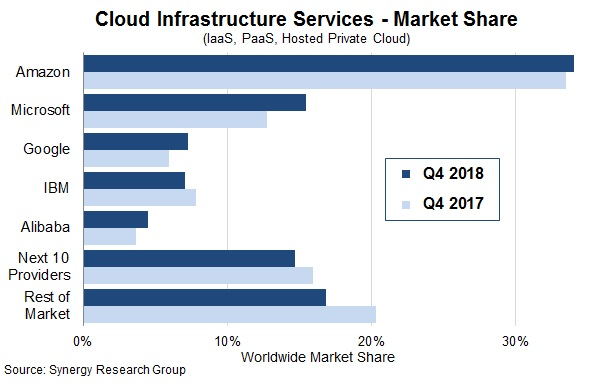
\includegraphics[width=\textwidth]{cloud_market_share}
\centering
\caption {Cloud market share by vendor}
\label{fig:cloud_market_share}
\end{figure}

Each of the top 4 cloud service providers - Amazon, Google, IBM , Microsoft, as well as smaller cloud providers that use the Openstack platform, provides not only the basic IaaS offering, but also an entire ecosystem of cloud based components - a PaaS, including networking, queues, databases, etc. Thus, it may be tempting to select one of these providers and build an entire software system that is based on a single vendor's offerings. This has the potential benefit of significantly simplifying system architecture and providing a single point of contact for troubleshooting.

It is, however, our opinion that taking such an approach would limit the appeal of the system to a wider user base. This opinion is driven by several considerations:

\begin{itemize}
\item The cloud computing market segment enjoys a great deal of growth and significant shifts in growth year-over-year as evidenced by Figure\ref{fig:cloud_market_share}, thus committing to a particular platform that is seen as a current market leader today, may limit the usability of the software when the chosen vendor falls out of the race in the future.
\item Because the market segment is highly competitive, end users can benefit significantly from limited time deals offered to them by cloud providers if they are flexible about what platform to deploy on.
\item Selecting one vendor induces vendor lock-in, possibly forcing adoption of inferior technologies to stay consistent with vendor choice.
\item Public and Private clouds typically operate on different software stacks. The nature of the data that is subject to scientific analysis may dictate where the analysis is able to proceed. 
\end{itemize}

On the other hand, supporting multiple cloud vendors has its own set of drawbacks:

\begin{itemize}
\item Handling multiple APIs for different vendors increases system complexity.
\item A solution that is vendor agnostic may lack certain capabilities that are only available to a subset of the vendors.
\item Some code duplication is inevitable when dealing with multiple platforms.
\end{itemize}

Based on considerations above we have taken the path of creating a cloud-agnostic system, i.e. one that will run on any major cloud providers, public, or private.

\subsection {Open Source License}

We adopt an open-source GPL v3.0 license for Butler.

\subsection {Overall System Design}

Overall, the Butler system can be thought of as being composed of four distinct sub-systems, each of which fulfills a number of requirements from Section \ref{sec:functional_requirements}. These sub-systems are:

\begin{description}
\item [Cluster Lifecycle Management] - This sub-system deals with the task of creating and tearing down clusters on various clouds, including defining Virtual Machines, storage devices, network topology, and network security rules. It implements requirements from sections \ref{sec:access_to_data}, and \ref{sec:access_to_compute_capacity}.
\item [Cluster Configuration Management] - This sub-system deals with configuration and software installation of all VMs in the cluster. It implements requirements from section \ref{sec:algorithm_implementation}.
\item [Workflow System] - The Workflow sub-system is responsible for allowing users to define and run scientific workflows on the cloud. This sub-system implements requirements from sections \ref{sec:workflow_definitions}, \ref{sec:workflow_engine}, and \ref{sec:system_of_record}.
\item [Operational Management] - This sub-system provides tools for ensuring continuous successful operation of the cluster, as well as for troubleshooting error conditions. It implements requirements stated in section \ref{sec:troubleshooting}
\end{description}

Each sub-system is described in full detail below.

\section{Cluster Lifecycle Management}

Before any computation can happen on the cloud a cluster of Virtual Machines is needed. The scope of Cluster Lifecycle Management includes:

\begin{itemize}
\item Defining hardware configuration for VMs
\item Defining initial basic software configuration for VMs
\item Defining storage devices
\item Defining network topology
\item Defining network security
\item Creating and Tearing down VMs
\end{itemize}

Detailed requirements for these capabilities are specified in sections \ref{sec:access_to_data}, and \ref{sec:access_to_compute_capacity}.

To fulfill these requirements in a cloud agnostic manner Butler utilizes a framework called Terraform, developed by Hashicorp.

\subsection{Terraform}

Terraform is an Open Source framework for cloud agnostic cluster lifecycle management, that has been built by Hashicorp Inc., a San Francisco, California based company, and is distributed via a Mozilla Public License. The source code for Terraform is hosted on Github at https://github.com/hashicorp/terraform, and at the time of this writing (September, 2016) the latest release of the software is version v0.7.3

Terraform uses a proprietary human and machine readable file format for specifying cluster configurations that is called HashiCorp Configuration Language (HCL). Using this language the end user can define a number of constructs for cluster management, most important among them are - providers, resources, and variables.

\subsubsection {Terraform Providers}

Terraform providers enable the framework to talk to different cloud provider APIs. Each provider is responsible for translating HCL configurations into cloud-specific API calls. At the time of this writing the following Providers are available:

\begin{multicols}{2}
\begin{itemize}
\item AWS
\item CenturyLinkCloud
\item CloudFlare
\item CloudStack
\item Cobbler
\item Datadog
\item DigitalOcean
\item DNSimple
\item Google Cloud
\item Heroku
\item Microsoft Azure
\item OpenStack
\item SoftLayer
\item Scaleway
\item Triton
\item VMware vCloud Director
\item VMware vSphere
\end{itemize}
\end{multicols}

Typically in order to use a particular provider the user needs to insert a provider block into their configuration file where they specify details relevant to communicating with the particular API in question, such as - endpoint URL, username, password, SSH keyname, API key, etc., as seen in Figure \ref{fig:terraform_aws_provider}. 

\begin{figure}[h]
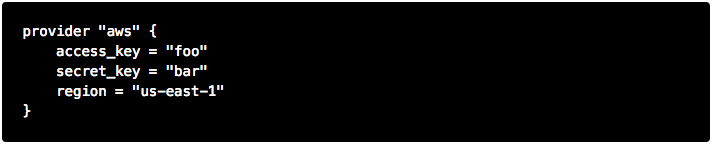
\includegraphics[width=\textwidth]{terraform_aws_provider}
\centering
\caption {Example Terraform provider configuration}
\label{fig:terraform_aws_provider}
\end{figure}

Once the user has specified a provider they can declare provider-specific Resources that define their cluster.

\subsubsection {Terraform Resources}

Resources represent different objects such as VMs, network routers, security groups, disks, etc., that the user can create on a given cloud. Each resource has a set of configuration options that can be specified to customize its behaviour. An optional \emph{count} attribute defines how many instances of the resource need to be created in the cluster.

\begin{figure}[h]
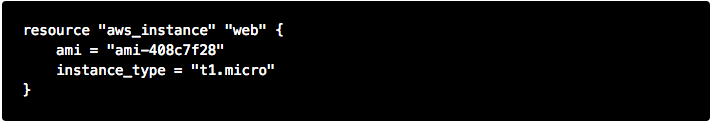
\includegraphics[width=\textwidth]{terraform_aws_instance}
\centering
\caption {Example Terraform AWS instance configuration}
\label{fig:terraform_aws_instance}
\end{figure}

Most Terraform configuration involves configuring resources.

\subsubsection {Terraform Variables}

Terraform variables are similar to variables in any other programming context. They consist of values assigned to labels, that can then be used for lookup elsewhere. Variables can be of string, list, or map type.

\begin{figure}[h]
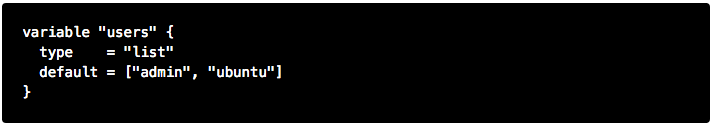
\includegraphics[width=\textwidth]{terraform_variable}
\centering
\caption {Example Terraform variable definition}
\label{fig:terraform_variable}
\end{figure}

Users typically specify variables in a separate configuration file and then use them throughout their cluster definition. 

One special case of using variables comes from specifying secret values such as passwords or secret keys that the use would not want to commit to a source repository. In this case, a variable can be referred to inside the configuration file, while being defined as an environment variable on the machine that Terraform will be executed on. The user prefixes the variable name with a special prefix -- \mintinline{sh}{TF\_VAR\_} which signals Terraform to parse the environment variable as a Terraform variable and allow appropriate substitution at runtime.

\subsubsection {Terraform Provisioners}

When a Virtual Machine is created the user may want to place certain files on it or run certain commands such as starting services or registering with a cluster manager, in order to bootstrap it. This purpose is served by Terraform Provisioners, which define code blocks that are executed on the target resource upon creation.

\begin{figure}[h]
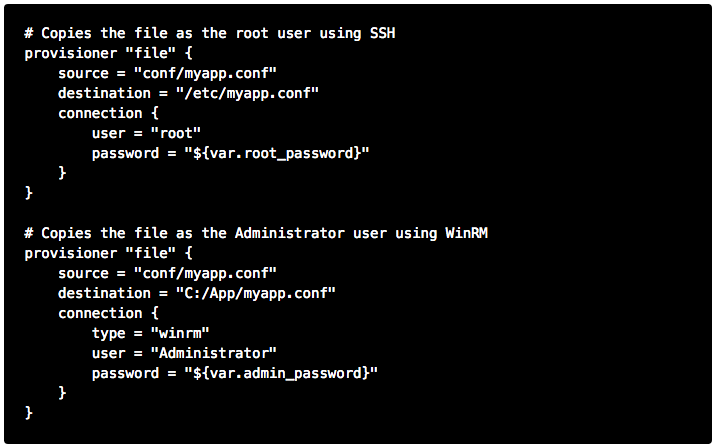
\includegraphics[width=\textwidth]{terraform_provisioner}
\centering
\caption {Example Terraform provisioner definition}
\label{fig:terraform_provisioner}
\end{figure}

\subsubsection {Terraform Installation}

Terraform is installed via a binary file downloaded from the Hashicorp website or by compiling the source code from github. It is a lightweight application that can be run from either the user's local machine, or from a special host on the target cloud environment. The application consists of a terraform CLI that the user can interact with by issuing shell commands. Typically users will combine their Terraform configuration files (stored in a source code repository) with a set of locally defined environment variables to set up and manage their clusters via the CLI.

\subsubsection {Terraform Cluster Lifecycle}

The key task of Terraform is to perform Create, Read, Update, and Delete on cluster resources. Create and Update operations are accomplished by issuing a \mintinline{sh}{terraform apply} command at the shell, while the shell is pointing to a directory with Terraform resource definitions. If the resources specified in the configuration do not yet exist, they are created. If the resource definitions have been changed since the last time \mintinline{sh}{terraform apply} was run, they will be brought into a state consistent with the latest definitions. This may involve updating existing resources where possible, or recreating them, where an update is not possible.

Terraform determines what changes need to be made in order to perform a successful Update via a file that is called a State file. This file specifies in a JSON format the current state of all infrastructure managed by Terraform. Running \mintinline{sh}{terraform apply} causes the tool to inspect current state and compare it to the target state, issuing any necessary commands to update current state to the target.

The Read operation simply displays the current Terraform state file via the \mintinline{sh}{terraform show} command.

The Delete operation is accomplished via the \mintinline{sh}{terraform destroy} command.

Other commands allow the user to validate the syntax of their configuration files, perform a dry run of resource creation, manually mark resources for recreation, and others.

\subsection {Terraform Use in Butler}

Butler comes with a set of Terraform configuration files that define templates for all of the VMs that constitute a functional Butler cluster, as well as configurations for network security. As previously stated a Butler cluster consists of Control VMs and Worker VMs - templates for both are available. The users are expected to adapt the templates as needed for their use case, providing their own credentials, cluster size, and other configurations.

\subsubsection {Example Configurations}


Listing \ref{lst:terraform_worker} demonstrates the Butler configuration file used to create 175 identical worker VMs that differ only by their hostname. 

The provider definition shows the procedure for setting up an OpenStack provider as well as demonstrating usage of variables where \mintinline{text}{user_name, tenant_name, and auth_url} are expected to come from a separate variable definition file, and  \mintinline{text}{password} is expected to come from an environment variable. 

The resource section shows definition of an OpenStack specific VM type \mintinline{text}{openstack_compute_instance_v2}, which has attributes like 
\mintinline{text}{image_id, flavor_name, security_groups, network}, etc. The  \mintinline{text}{connection} definition within the resource specifies how users will be able to connect to the newly created VMs. In this case it is accomplished via SSH using passwordless key-based authentication via a pass-through bastion host on the cloud.

Of further interest is the mechanism by which the creation of multiple instances of the same type is accomplished. The resource definition admits a \mintinline{text}{count} attribute which specifies how many instances need to be created. Furthermore, a \mintinline{text}{count.index} property keeps track of which instance is being created at run-time and can be used to provide unique hostnames to each instance as follows -   \mintinline{text}{name = "\${concat("worker-", count.index)}"}.

Lastly, the \mintinline{text}{provisioner} section runs a set of commands that provide initial configuration for the new host upon first bootup. These include installing and running the Saltstack service which is used for configuration management, setting up machine roles  that determine what capabilities this VM will have in the cluster, and telling the VM what the IP address of the cluster manager is.

Listing \ref{lst:terraform_security_group} demonstrates the definition of a security group under OpenStack. VMs that are put into this security group will have two network security rules applied to them - opening port 22 for SSH communication between hosts, and opening ports 4505-4506 to enable Saltstack communication.

\section{Cluster Configuration Management}

Although a Cluster Lifecycle Management system like Terraform can create a Virtual Machine using a machine image, and even run some initial configuration commands, it is not enough to successfully manage the configuration of an entire large-scale computational cluster. Machines in the cluster will have hundreds of programs installed and configured on them, oftentimes with intricate interdependencies, and inter-machine communication requirements. Moreover, different operating systems will typically have different commands and mechanisms for installing and configuring software, and it would be unnecessarily limiting to require the end user to commit to a particular flavour of operating system. To help accomplish these tasks, as well as detailed requirements from Section \ref{sec:algorithm_implementation} we need to enlist the help of a Cluster Configuration Management system.

Several open source Configuration Management systems are available on the market today, the main options are:

\begin{itemize}
\item Chef
\item Puppet
\item Ansible
\item Saltstack
\end{itemize}

Each system has benefits and drawbacks and a dedicated user base. Table \ref{tab:configuration_management} compares the github codebases for these products in terms of number of stars, number of contributors, and number of commits in the last year. 

\begin{table}[H]
\renewcommand{\arraystretch}{1.2} 
\centering
\caption{Configuration Management Frameworks github summary}
\label{tab:configuration_management}
\begin{tabu} to \linewidth{XX[,r]X[,r]X[,r]}
\toprule
Product & Number of Stars & Number of Contributors & Commits in last 12 months\\
\midrule
Chef & 4417 & 474 & 1861 \\
Puppet & 4151 & 431 & 1474\\
Ansible & 18720 & 1469 & 3483\\
Saltstack & 6850 & 1580 & 9769 \\
\bottomrule
\end{tabu}
\end{table}

As can be seen from the data, all four are fairly active and stable projects, Ansible appears to be the most popular tool, and Saltstack is most actively developed, based on number of commits and contributors. Both Puppet and, Chef come from the first generation of configuration management tools having been initially released in 2005 and 2009 respectively, and suffering somewhat from having been trailblazers in the field. The largest complaint against both systems has been their unnecessary complexity and steep learning curve. Ansible and Saltstack, on the other hand, can be thought of as the second generation of configuration management systems, first released in 2012 and 2011, respectively. Both are based on simple to read and understand YAML-based configuration files, and have generally enjoyed greater adoption in the field.

For Butler we selected Saltstack to fulfill configuration management duties. The chief reason for selecting Saltstack over Ansible was that Saltstack appears to perform better when managing large clusters, whereas Ansible is known to suffer from increased lag in these scenarios. Since we anticipate to operate Butler clusters with several hundred VMs at a time we settled our choice on Saltstack.

\subsection {Saltstack}

Saltstack is an open source product that has been developed specifically for large scale configuration management. The key paradigm that Saltstack implements is declarative configuration management. This means that the user specifies declaratively, in a configuration file, what state a particular Virtual Machine should be in (in terms of installed and running software), and the Saltstack engine automatically compares the desired state to the actual state and carriers out the necessary actions to match the two. As an added benefit, it does so in an operating system agnostic manner. In contrast to scripts that operate in an imperative manner via statements like \mintinline{sh}{yum install apache} or \mintinline{sh}{service httpd start}, Saltstack files describe a desired state with statements like \mintinline{yaml}{service.running} and \mintinline{sh}{package.installed}. In the first case, the script would try to install the package a second time, even if it was present, whereas Saltstack first figures out whether the package is installed and only installs it if it is missing.

\subsubsection {Saltstack Architecture}

The Saltstack architecture consists of a cluster of Minions that are managed by one or many Masters. A Master is a Virtual Machine that acts as the authority on configuration definitions within the cluster and issues commands that the Minions run. A Master needs to have configuration definitions stored locally on its disk or be available through a git repository. It runs a special salt-master daemon, and requires certain network ports to be open for communication.

Minions need to know how to find the master on the network (by IP address). Each Minion generates a unique key and presents it to the Master. Once a Master accepts the Minion's key there is a handshake and the Minion falls under the Master's control. The Minion runs a salt-minion daemon.

Each Minion can have a number of roles assigned to it and the Master maintains mappings between roles and configurations. Once the Master has determined what roles a Minion has it can issue the necessary commands to apply relevant configurations to the Minion. 

\subsubsection {Saltstack Data Model}

The Saltstack Data Model has four main concepts - State, Pillar, Grain, and Mine. We consider each in turn.

\paragraph{A Salt State} is simply the definition for what state some piece of infrastructure should be in. For instance, if we want some server in our cluster to be in the state of running a PostgreSQL database we need to do the following:

\begin{enumerate}
\item Create a postgres user
\item Create a postgres directory
\item Download the postgres-server package
\item Install the postgres-server package
\item Initialize the database
\item Override default configuration settings
\item Start the server
\end{enumerate}

The corresponding Salt state that accomplishes the same task looks as follows:

\captionof{listing} {Salt state for setting up a PostgreSQL server. \label{lst:salt_state_postgres}}
\begin{minted}
[
breaklines=true,
linenos,
fontsize=\footnotesize,
frame=lines,
framesep=2mm,
baselinestretch=1.2
]
{yaml}
install_server:
  pkg.installed:
    - name: postgresql95-server.x86_64
    
initialize_db:
  cmd.run:
    - name: /usr/pgsql-9.5/bin/postgresql95-setup initdb
    - unless: stat /var/lib/psql/9.5/data/postgresql.conf

/var/lib/pgsql/9.5/data/postgresql.conf:
  file.managed:
    - source: salt://postgres/config/postgresql.conf
    - user: postgres
    - group: postgres
    - mode: 600
    - makedirs: True

    
start_server:    
  service.running:
    - name: postgresql-9.5
    - watch:
      - file: /var/lib/pgsql/9.5/data/*
\end{minted}

The code for a Salt state is placed in a special file called an \emph{.sls} file. All of the state definitions that the system knows about are arranged into a folder hierarchy where the name of each folder defines the name of the state. The state definition is then located inside the folder in a file named \emph{init.sls}, as demonstrated in Figure \ref{fig:salt_state_airflow} for the Airflow Workflow engine.

\begin{figure}[H]
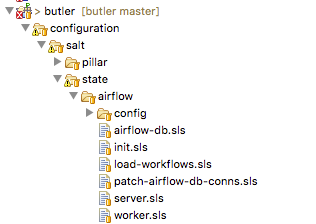
\includegraphics{salt_state_airflow}
\centering
\caption {Salt state files for Airflow Workflow Engine}
\label{fig:salt_state_airflow}
\end{figure}

Several related states (such as those describing different installations of the same program) can be grouped together under the same parent state. Then each sub-state is placed into its own \emph{.sls} file under the main state's folder, with the name of the file giving rise to that state's name. Figure \ref{fig:salt_state_airflow} provides an example of this scenario where in addition to the main \emph{airflow} state there are sub-states such as \emph{airflow.server}, \emph{airflow.worker}, \emph{airflow.load-workflows} etc. Note that sub-states are referenced via \emph{name\_of\_parent\_state.name\_of\_substate}.

\paragraph{A Salt Pillar} is a set of key-value pairs that are stored encrypted on a Minion and constitute look-up values that are relevant for that Minion's configuration. Examples of Pillar values can be usernames and passwords, locations of certain files, etc. A State definition can refer to Pillar values when configuring a system, and two identical VMs that differ only by their Pillar values will be parametrized differently at configuration time. One example of this is setting up the same server in a QA environment vs. Production. In QA the server may point to a test data directory with especially constructed data files, for testing purposes, whereas in Production the server would point to the actual data directory with real samples.

The Pillar are organized similar to States in a folder hierarchy of \emph{.sls} files. Figure \ref{fig:salt_pillar_hierarchy}

\begin{figure}[H]
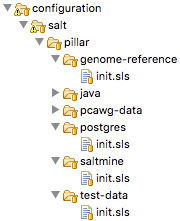
\includegraphics{salt_pillar_hierarchy}
\centering
\caption {A set of Salt Pillar definitions}
\label{fig:salt_pillar_hierarchy}
\end{figure}

Listing \ref{lst:salt_pillar_test_data} shows an example Pillar definition where information related to finding test data is stored.

\paragraph{Salt Grains} are bits of information Salt collects about Minion state or characteristics. They include things like:

\begin{itemize}
\item Minion IP address
\item Amount of RAM on minions
\item Minion hostname
\item Minion network interfaces
\end{itemize}

and others. The Grains can be used to introspect and pass on configuration values (like IP address) that are not known in advance. One of the most important uses of Grains is the ability to assign roles to a Minion via the Grains mechanism. Since roles define what states are eventually applied, adding or removing a role to a VM via Grains has a very significant side-effect. 

\paragraph{The Salt Mine} is a centralized repository of information about the state of all Minions that is stored on the Master. Information is passed into the Mine from Grains and other sources. It can then be used inside state definitions to further customize the system.  

Listing \ref{lst:salt_mine} demonstrates how the Jinja templating engine is used to look up the IP Address of servers in the cluster that have the \mintinline{text}{consul-server} or\mintinline{text}{consul-bootstrap} role. Then this IP Address is used inside a State definition to join a cluster of similar machines. Without the Mine, this particular Minion would not know who to ask for this IP Address, but because the Mine is centralized on the Salt Master host this lookup is possible.

\paragraph{The Top File} is the mechanism used in Saltstack to specify what VMs will have what States applied to them. The Top File provides a lot of flexibility in terms of how to accomplish this mapping. Mappings can be accomplished via hostname or any Grains values, and it allows regular expressions. The most flexible and, thus preferred, method of mapping States to VMs is via Roles.

Listing \ref{lst:salt_top_file} demonstrates how the State mapping to Roles is accomplished in a Top File. Based on this Top File all VMs will get the \mintinline{text}{consul, dnsmasq, and collectd} states. VMs with the \mintinline{text}{monitoring-server} role will get \mintinline{text}{influxdb, and grafana}, and VMs with the \mintinline{text}{job-queue} role will get the \mintinline{text}{rabbitmq} State.

\subsubsection{Controlling Saltstack}

Control over the cluster is exercised from the Salt Master. The user establishes a shell session on the Salt Master and issues commands via the Saltstack CLI. Each command has the following syntax:

\mintinline{text}{"salt target_expression command_expression"} where:

\mintinline{text}{salt} is the name of the Salt CLI.

\mintinline{text}{target_expression} is an expression that determines what VMs to apply the command to. It can be a logical expression that combines hostnames, grains, and regular expressions.

\mintinline{text}{command_expression} is an expression that determines what actual command to run on the targeted VMs. The \mintinline{text}{command_expression} can be as simple as running a shell command on the target VMs, or it can apply a particular named state via the \mintinline{text}{state.apply} command, or it can apply all matching states via the special \mintinline{text}{state.highstate} command.

For example, \mintinline{sh}{salt -G 'roles:worker' state.apply airflow.patch-airflow-db-conns} applies the \mintinline{text}{airflow.patch-airflow-db-conns} state to all VMs that have the \mintinline{text}{worker} role.

\subsection{Saltstack Use in Butler}

Butler uses Saltstack extensively in order to install software on the cluster. This includes software that is required to run Butler itself, as well as installing scientific algorithms required for running actual workflows on Worker VMs (as specified in Section \ref{sec:algorithm_implementation} of the Requirements chapter). As seen in Figure \ref{fig:salt_states} the Saltstack configuration in Butler consists of a set of State and Pillar definitions along with the Top Files that map these States and Pillar to various VMs in the cluster. These definitions are enough to configure a completely functional Butler cluster from a single shell command.

\begin{figure}[H]
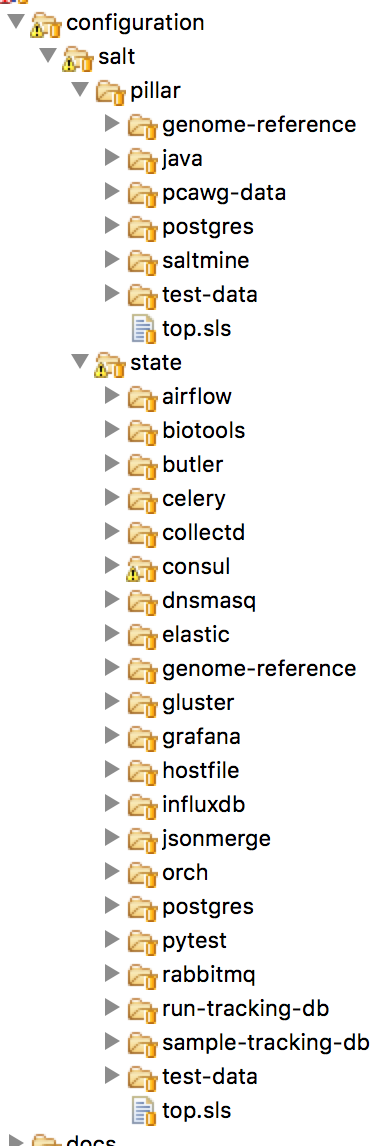
\includegraphics{salt_states}
\centering
\caption {Salt States and Pillar used in Butler}
\label{fig:salt_states}
\end{figure} 

A typical Butler installation that can support a cluster of up to 1500 CPUs consists of four Control VMs in addition to the Worker VMs, each has a separate Terraform profile. The Control VMs are:

\begin{description}
\item[salt-master] - This machine is the configuration master node. Because this workload is typically only heavy during cluster setup, the same VM also acts as the Monitoring Server during regular operation.
\item[db-server] - This VM hosts all the databases that Butler uses.
\item[job-queue] - This VM hosts a Queue for distributed task processing.
\item[tracker] - This VM hosts all of the workflow engine components, as well as Analysis Tracking.
\end{description}

All of the VMs in the cluster get the following basic configurations mapped in the Top File:

\begin{minted}
[
breaklines=true,
]
{yaml}
  '*':
    - consul
    - dnsmasq
    - collectd
    - elastic.filebeat
    - elastic.packetbeat
\end{minted}

\begin{description}
\item [consul] - A framework used to Service Discovery which will be described in detail in Section \ref{sec:design_consul}
\item [dnsmasq] - A local DNS server, to enable name lookups.
\item [collectd] - A Metrics collection agent.
\item [elastic.filebeat] - A server log harvester.
\item [elastic.packetbeat] - A network event log harvester.
\end{description}

\subsubsection{Setting up the Salt Master}

The first order of business when setting up a new Butler cluster is to bootstrap the Salt Master VM, as this VM is responsible for configuring and installing the software of all the other machines, including itself.

A Butler VM is typically provisioned from a base VM image, which has little more than the barebones OS, using Terraform. In the case of the Salt Master, the salt-master daemon is installed via Terraform's \mintinline{text}{remote-exec} provisioner. Salt's \mintinline{sh}{highstate} command is then executed on the master itself in order to fully initialize it. At that point the Salt Master is ready to configure other machines that are part of the cluster.

As previously mentioned, because the load on the Salt Master is typically only high during initial cluster setup and during short bursts during normal operation, the Salt Master VM typically has another Saltstack Role mapped to it - that of the Monitoring Server. This role installs monitoring components that will be described in detail in Section \ref{sec:operational_management}

\subsubsection {Setting up Other Butler Control VMs}

The DB Server VM has a db-server Role mapped to it. Because databases are resource intensive software that does not scale horizontally, this VM does not have other roles within the cluster.

\begin{minted}
[
breaklines=true,
]
{yaml}
  'G@roles:db-server':
    - postgres
    - run-tracking-db
    - grafana.createdb
    - airflow.airflow-db
    - sample-tracking-db
\end{minted}

The Top File mapping of States to the \mintinline{text}{db-server} role ensures that the PostgreSQL DB Server is installed as well as a number of databases that are used by Butler for tracking scientific analyses, workflow statuses, analysis samples, and performance metrics.

The Job Queue VM has a \mintinline{text}{rabbitmq} state mapped to it in the Top File, to install the RabbitMQ queueing system.

The Tracker VM correspondingly has a \mintinline{text}{tracker} role and the following state mappings:

\begin{minted}
[
breaklines=true,
]
{yaml}
  'G@roles:tracker':
    - airflow
    - airflow.load-workflows
    - airflow.server
    - jsonmerge
    - butler
\end{minted}

These states install and configure the Airflow Workflow engine, load available workflows, and check out and install the Butler codebase from github. The codebase is needed to run the Butler CLI which is used to set up and manage Butler analyses. Thus, most interactions the users have with Butler occur from the Tracker VM via the Butler CLI.

\subsubsection {Setting up Butler Workers}

While Control VMs will be quite similar from one installation of Butler to the next, the Worker VMs will differ quite a bit, depending on what types of analyses are anticipated to be performed. The base Worker VM has the \mintinline{text}{worker} role which simply allows such VMs to run workflows in principle by installing the necessary components of the workflow engine and Butler Analysis Tracker.

\begin{minted}
[
breaklines=true,
]
{yaml}
  'G@roles:worker':
    - dnsmasq.gnos
    - celery
    - airflow
    - airflow.load-workflows
    - airflow.worker
    - butler
\end{minted}

The actual scientific algorithms that are required for running particular analyses are installed onto Workers via additional Roles and States. Because the initial Butler implementation is focused on bioinformatics workflows there already exist predefined states for some common bioinformatics tools. An example of such a Role and States can be seen in the Top File mapping below:

\begin{minted}
[
breaklines=true,
]
{yaml}
  'G@roles:germline':
    - biotools.freebayes
    - biotools.htslib
    - biotools.samtools
    - biotools.delly
\end{minted}

\subsubsection {Customizing Butler Configuration}

When Butler is used in different environments, configurations need to change, because of differences in OS, network, and underlying analyses. In order to accomplish this, the users will typically need to create their own source code repository that will coexist with the base Butler repository. Inside that repository will be custom definitions or workflows, analyses, as well as configurations. Where it is possible to configure the system entirely via Pillar, the user should define these custom Pillar settings in their repository, but when customizations to the States are required, the user should copy the State definition from the base Butler repository into their own and customize as necessary. They should then make sure that the customized states are available to Saltstack by downloading them to the Salt Master VM.

When it comes to installing new scientific algorithms for the purposes of running workflows, the users should define any new States and Roles as necessary, and then assign them to the Worker VMs prior to calling \mintinline{text}{highstate} to ensure the software get installed properly. 

\section{Workflow System}\label{sec:design_workflow_system}
\subsection{Workflow System Overview}
Running scientific workflows at scale is the reason for Butler's existence. Thus, the Workflow Engine lies at the heart of the entire system. To fulfill the requirements specified in Section \ref{sec:workflow_engine} we have selected the Airflow Workflow Engine developed by Airbnb. 

\subsubsection {Airflow Architecture}

The architecture of Airbnb Airflow lends itself well to large-scale distributed processing of tasks, due to the loosely coupled nature of the system. The key component at the heart of Airflow is the Airflow Scheduler. The airflow-scheduler is a service that runs perpetually on a VM and examines the state of all running workflows. All workflow tasks that meet the preconditions for being runnable are immediately "scheduled" for execution. In the context of Airflow scheduling means depositing the task into a queue (running on a separate Queue Server VM) from which a Worker VM can eventually pick it up. The Worker VMs run an airflow-worker service which periodically polls the task queue for available tasks and when the task is runnable by a particular Worker, that Worker consumes the task message from the queue and assumes execution. In order to keep track of the status of Workers and workflow execution each Worker periodically sends heartbeat messages to the Scheduler to communicate state. The state is persisted by the Scheduler to a PostgreSQL database which runs on a DB Server VM.

Additional state information related to tracking scientific analyses is written to a separate PostgreSQL database which runs on the same DB Server.

The user can communicate with and commandeer Airflow via the Airflow CLI, as well as a Web UI. The Web UI is provided via the airflow-flower, and airflow-webserver services which can run on the same VM as the Scheduler or on a separate VM, depending on system load.
 
\subsection{Workflow Definition}

Requirements for workflow definitions are specified in Section \ref{sec:workflow_definitions} of this document. Conceptually, an Airflow workflow is a Directed Acyclic Graph whose vertices represent tasks and edges indicate task sequence. In its implementation an Airflow workflow is a Python program that can use any Python language construct or library. This allows the users to create workflows of arbitrary complexity and functionality.

When authoring workflows the user needs to create an instance of the \mintinline{python}{DAG} class

\begin{minted}[breaklines=true]{python}
class airflow.models.DAG(dag_id, schedule_interval=datetime.timedelta(1), start_date=None, end_date=None, full_filepath=None, template_searchpath=None, user_defined_macros=None, default_args=None, concurrency=16, max_active_runs=16, dagrun_timeout=None, sla_miss_callback=None, params=None)
\end{minted}

The key parameters to the \mintinline{python}{DAG} constructor are:

\begin{description}
\item [dag\_id] - Unique identifier for the workflow.
\item [schedule\_interval] - How often the workflow is executed.
\item [default\_args] - A dictionary of arguments that is passed to tasks within this workflow.
\item [concurrency] - Maximum number of concurrent workflow tasks.
\item [max\_active\_runs] - Maximum number of simultaneously active workflow runs.
\end{description}

Once the \mintinline{python}{DAG} is created the user can define workflow tasks. Each task is encoded as a subclass of Operator. There are three main types of Operator in Airflow:

\begin{itemize}
\item Operators that represent actions that need to be taken.
\item Transfer operators which represent movement of data.
\item Sensor operators which poll the environment for a specified condition.
\end{itemize} 

All Operators are derived from the \mintinline{python}{BaseOperator} class.

\begin{minted}[breaklines=true]{python}
class airflow.models.BaseOperator(task_id, owner='airflow', email=None, email_on_retry=True, email_on_failure=True, retries=0, retry_delay=datetime.timedelta(0, 300), retry_exponential_backoff=False, max_retry_delay=None, start_date=None, end_date=None, schedule_interval=None, depends_on_past=False, wait_for_downstream=False, dag=None, params=None, default_args=None, adhoc=False, priority_weight=1, queue='default', pool=None, sla=None, execution_timeout=None, on_failure_callback=None, on_success_callback=None, on_retry_callback=None, trigger_rule=u'all_success', resources=None, *args, **kwargs)
\end{minted}

An Operator can take many parameters, the most important ones are:

\begin{description}
\item [dag] - Reference to the DAG this task belongs to.
\item [task\_id] - Unique identifier for the task.
\item [retries] - Along with several other parameters, this controls retry behaviour in case of failures.
\item [priority\_weight] - Relative importance of scheduling this task compared to other tasks.
\item [trigger\_rule] - Condition under which this task triggers. One of - all\_success | all\_failed | one\_success | one\_failed. This condition evaluates the state of tasks that are upstream of this one.
\end{description}

A large number of Operator implementations are available that simplify the creation of arbitrary workflows. Some of these are:

\begin{description}
\item [BashOperator] - Execute a shell script.
\item [PythonOperator] - Execute a Python callable.
\item [EmailOperator] - Send an email.
\item [ExternalTaskSensor] - Wait for a task in a different workflow to complete.
\item [HdfsSensor] - Wait for a file to appear in HDFS.
\item [HiveOperator] - Execute a Hive query.
\item [SimpleHttpOperator] - Make a call to an HTTP endpoint.
\item [PostgresOperator] - Execute a PostgreSQL query.
\item [DockerOperator] - Execute a command inside a Docker container.
\item [SSHExecuteOperator] - Execute commands on a remote host.
\end{description}

In practice we find that the \mintinline{python}{PythonOperator} is the most versatile as it provides the ability to call arbitrary Python code which can, in turn, accomplish any of the tasks of the other operators if necessary.

Once tasks are defined their dependencies can be established by calling \mintinline{python}{task_2.set_upstream(task_1)} or \mintinline{python}{task_1.set_downstream(task_1)}. The \mintinline{python}{set_upstream()} and \mintinline{python}{set_downstream()} methods also accept lists of tasks for bulk assignment.

When a workflow is executed each task definition is transformed into a task instance - a task that is running at some point in time. Although the entire workflow may be defined in the same source file, Airflow makes no guarantees about where each task instance will run. Once a task instance is placed into the task queue technically any worker can pick up and execute that task. On the one hand this provides a limitation because it makes it difficult for tasks to exchange information between each other (due to possible remoteness), on the other hand, this model promotes scalability as it limits dependencies between tasks and simplifies scheduling.

Because no assumptions are made about which worker will run which tasks, each worker needs to have a copy of all workflow definitions that are active in the system. Furthermore, any programs that may be invoked inside a task also need to be installed on the workers. Unfortunately, Airflow does not provide any mechanisms for declaring and checking whether the programs a workflow depends on are installed and available prior to task instance runtime. This means that most bugs and issues related to dependency installation are only discovered when an actual workflow is running and fails. Thankfully, the job of installing and configuring dependencies is made relatively easy by the Butler Configuration Management System. 

\subsection{Analysis Tracker} 
\label{sec:analysis_tracker}

As described in Section \ref{sec:system_of_record} of the requirements, a System of Record is necessary to track the scientific analyses that are undertaken using the Butler system. To fulfill these requirements we have built an Analysis Tracker module into Butler. The goal of this module is to allow the user to define analyses, specify what workflows are part of these analyses, and track the status and execution of Analysis Runs - instances of running a particular workflow on a particular data sample within the context of an Analysis. To accomplish this we have established a Run Tracking Database on PostgreSQL to persist the data, we have built a tracker Python module that implements the management of these objects, and finally, we have built a set of standard workflow tasks that the users can insert into their workflows in order to report progress to the Analysis Tracker.

\subsubsection{tracker Python Module}

The layout of the tracker module can be seen in Figure \ref{fig:tracker_module_files} below:

\begin{figure}[H]
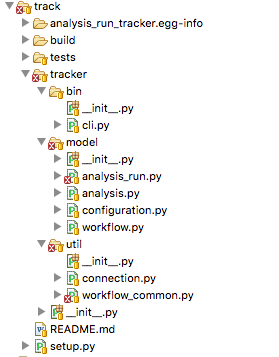
\includegraphics{tracker_module_files}
\centering
\caption {File hierarchy of the tracker module}
\label{fig:tracker_module_files}
\end{figure}

At the root of the hierarchy are the README file and the module installation script \mintinline{sh}{setup.py}. Inside the \mintinline{sh}{bin} directory is the Analysis Tracker CLI implementation - \mintinline{sh}{cli.py}. Inside the \mintinline{sh}{model} directory lies the implementation of the main model objects - Workflow, Analysis, Analysis Run, and Configuration. We describe the first three of these objects in detail in this section and the last one in Section \ref{sec:workflow_configuration_design}. Inside the \mintinline{sh}{util} directory are utility functions -  \mintinline{sh}{connection.py} for connecting to the Run Tracking Database, and  \mintinline{sh}{workflow_common.py} for implementations of common workflow tasks.

The overall model can be seen in Figure \ref{fig:analysis_tracker_model}

\begin{figure}[H]
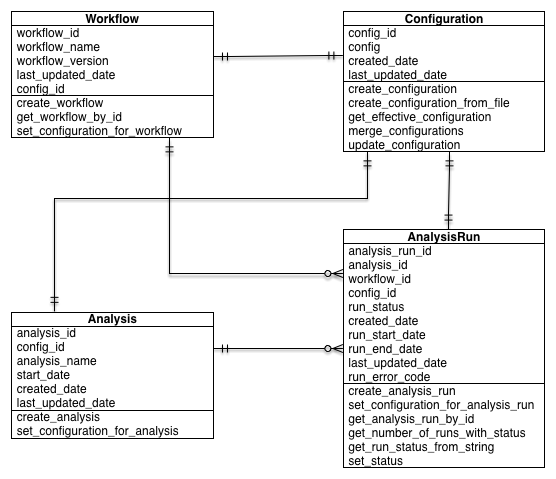
\includegraphics[width=\textwidth]{analysis_tracker_model}
\centering
\caption {UML model of the Analysis Tracker.}
\label{fig:analysis_tracker_model}
\end{figure}

\paragraph{The Workflow} object represents a workflow definition. Every workflow managed by Butler should have a corresponding Workflow object representing it. It has the following fields:

\begin{description}
\item [workflow\_id (UUID)] - This is the unique identifier of this workflow.
\item [workflow\_name (String)] - This is a human-friendly name for the workflow.
\item [workflow\_version (String)] - It is important to record what version of a workflow is being used, as updates are frequently made during the workflow lifecycle.
\item [last\_updated\_date (datetime)] - Timestamp of last update to this object.
\item [config\_id (UUID)] - The unique identifier of the corresponding Configuration object.
\end{description}

The Workflow object implements the following methods:

\begin{description}
\item [\mintinline{python}{create_workflow(workflow_name, workflow_version, config_id)}] - Create a new workflow object with given name, version, and configuration.
\item [\mintinline{python}{get_workflow_by_id(workflow_id)}] - Retrieve the workflow with ID \mintinline{python}{workflow_id} from persistent storage.
\item [\mintinline{python}{set_configuration_for_workflow(workflow_id, config_id)}] - Update the workflow configuration to configuration with ID \mintinline{python}{config_id}.
\end{description}

\paragraph{The Analysis} object represents a scientific analysis. It serves the purpose of aggregating the running of a set of workflows on a set of data samples together into a single unit of execution that can be referred to for organization purposes. The Analysis has the following fields.

\begin{description}
\item [analysis\_id (UUID)] - This is the unique identifier of this Analysis.
\item [analysis\_name (String)] - This is a human-friendly name for the Analysis.
\item [start\_date (datetime)] - Date of when the Analysis is meant to start.
\item [created\_date (datetime)] - Date of when the Analysis was created.
\item [last\_updated\_date (datetime)] - Timestamp of last update to this object.
\item [config\_id (UUID)] - The unique identifier of the corresponding Configuration object.
\end{description}

The Analysis object has the following methods:

\begin{description}
\item [\mintinline{python}{create_analysis(analysis_name, start_date, config_id)}] - Create a new Analysis object with given name, \mintinline{python}{start_date}, and configuration.
\item [\mintinline{python}{set_configuration_for_analysis(analysis_id, config_id)}] - Update the Analysis configuration to configuration with ID \mintinline{python}{config_id}.
\end{description}

\paragraph{The AnalysisRun} object represents the invocation of a particular Workflow on a particular Data Sample, within the scope of a particular Analysis. This object is central to the Analysis Tracking functionality. The AnalysisRun object has the following fields:

\begin{description}
\item [analysis\_run\_id (UUID)] - This is the unique identifier of this Analysis Run.
\item [analysis\_id (UUID)] - This is the unique identifier of the Analysis for this Analysis Run.
\item [workflow\_id (UUID)] - This is the unique identifier of the Workflow for this Analysis Run.
\item [run\_status (int)] - This integer field indicates the status of this Analysis Run. Status can be one of \mintinline[breaklines=true]{python}{RUN_STATUS_READY, RUN_STATUS_SCHEDULED, RUN_STATUS_IN_PROGRESS, RUN_STATUS_COMPLETED, RUN_STATUS_ERROR}.
\item [created\_date (datetime)] - Date of when the Analysis Run was created.
\item [run\_start\_date (datetime)] - Date of when the Analysis Run started.
\item [run\_end\_date (datetime)] - Date of when the Analysis Run ended.
\item [last\_updated\_date (datetime)] - Timestamp of last update to this object.
\item [run\_error\_code (int)] - Integer pointing to an error code of Runs that ended in error.
\item [config\_id (UUID)] - The unique identifier of the corresponding Configuration object.
\end{description}

The Analysis Run object implements the following methods:

\begin{description}
\item [\mintinline{python}{get_run_status_from_string(run_status_string)}] - Translate string-based run statuses into int-based ones.
\item [\mintinline{python}{create_analysis_run(analysis_id, config_id, workflow_id)}] - Create an AnalysisRun and store in the database.
\item [\mintinline{python}{set_configuration_for_analysis_run(analysis_run_id, config_id)}] - Update the AnalysisRun configuration to configuration with ID \mintinline{python}{config_id}.
\item [\mintinline{python}{get_analysis_run_by_id(analysis_run_id)}] - Get the Analysis Run with ID \mintinline{python}{analysis_run_id}.
\item [\mintinline{python}{set_ready(my_run)}] - Set the status of a given analysis run to \mintinline{python}{RUN_STATUS_READY}. Only possible if the current status is not \mintinline{python}{RUN_STATUS_IN_PROGRESS}.
\item [\mintinline{python}{set_scheduled(my_run)}] - Set the status of a given analysis run to \mintinline{python}{RUN_STATUS_SCHEDULED}. Only possible if the current status is \mintinline{python}{RUN_STATUS_READY}.
\item [\mintinline{python}{set_in_progress(my_run)}] - Set the status of a given analysis run to \mintinline{python}{RUN_STATUS_IN_PROGRESS}. Only possible if the current status is \mintinline{python}{RUN_STATUS_SCHEDULED}.
\item [\mintinline{python}{set_completed(my_run)}] - Set the status of a given analysis run to \mintinline{python}{RUN_STATUS_COMPLETED}. Only possible if the current status is \mintinline{python}{RUN_STATUS_IN_PROGRESS}.
\item [\mintinline{python}{set_error(my_run)}] - Set the status of a given analysis run to \mintinline{python}{RUN_STATUS_ERROR}.
\item [\mintinline{python}{get_number_of_runs_with_status(analysis_id, run_status)}] - Returns the number of AnalysisRuns of a given status.
\end{description}

As can be seen from the description of the methods of \mintinline{python}{AnalysisRun} these objects follow a particular lifecycle that is represented by their \mintinline{python}{status} attribute. The rules that govern allowable status transitions are encoded within the series of \mintinline{python}{set_*} methods and are summarized in Figure \ref{fig:analysis_run_status_transitions}

\begin{figure}[H]
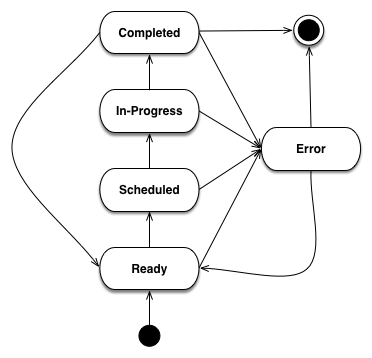
\includegraphics{analysis_run_status_transitions}
\centering
\caption {State Diagram of Analysis Run Status Transitions.}
\label{fig:analysis_run_status_transitions}
\end{figure}

When an \mintinline{python}{AnalysisRun} is first created it does not have a status. Once the object is fully initialized it is given a Ready status, indicating that it is ready to be scheduled for execution. Once the Scheduler has scheduled the Run for execution it is given a Scheduled status. When workflow execution starts the Run is marked In-Progress. Once the Run is successfully completed it enters a Completed status. If, at any point, the Run encounters an error condition it cannot recover from, the Run Status is set to Error. When the error condition is addressed the Run status should be set to Ready so that it can start from the beginning.

\paragraph{The workflow\_common.py} file within the tracker module contains a number of convenience functions that workflows can use to perform common tasks. Currently the following functions are supported:

\begin{description}
\item [\mintinline{python}{get_config(kwargs)}] - Get the Configuration supplied to this Workflow.
\item [\mintinline{python}{get_sample(kwargs)}] - Get the sample assigned to this Workflow.
\item [\mintinline{python}{start_analysis_run(**kwargs)}] - Mark the Analysis Run of this Workflow In-Progress.
\item [\mintinline{python}{complete_analysis_run(**kwargs)}] - Mark the Analysis Run of this Workflow Complete. 
\item [\mintinline{python}{set_error_analysis_run(**kwargs)}] - Mark the Analysis Run of this Workflow as Error.
\item [\mintinline{python}{validate_sample(**kwargs)}] - Test whether the sample files are accessible to the workflow.
\item [\mintinline{python}{call_command(command, command_name, cwd=None)}] - Wrapper around Python's \mintinline{python}{subprocess.call} method that captures logging information.
\item [\mintinline{python}{compress_sample(result_filename, config)}] - Compress the sample with gzip.
\item [\mintinline{python}{uncompress_gzip_sample(result_filename, config)}] - Uncompress the sample.
\end{description}

Every workflow should begin by starting the corresponding Analysis Run, and finish by completing it to ensure appropriate tracking of information throughout the system.

\paragraph{The connection.py} file is also a key component of the tracker module because it provides a means to communicate with the Run Tracking Database.

The Run Tracking Database is a PostgreSQL database this is set up to persist all of the Analysis related information into permanent storage in order to fulfill the System of Record requirements of Section \ref{sec:system_of_record}. Specifically, the Run Tracking Database contains a relational model that corresponds to the Python objects described above. These tables are as follows:

\begin{table}[H]
\renewcommand{\arraystretch}{1.2} 
\centering
\begin{tabular}{@{}lll@{}}
\toprule
Column Name & Type & Constraint\\
\midrule
workflow\_id & serial & PRIMARY KEY\\
config\_id & uuid & REFERENCES configuration(config\_id)\\
workflow\_name & varchar(255) & \\
workflow\_version & varchar(255) & \\
created\_date & timestamp\\
last\_updated\_date & timestamp\\
\bottomrule
\end{tabular}
\caption{Database table workflow}
\end{table}

\begin{table}[H]
\renewcommand{\arraystretch}{1.2} 
\centering
\begin{tabular}{@{}lll@{}}
\toprule
Column Name & Type & Constraint\\
\midrule
analysis\_id & serial & PRIMARY KEY\\
config\_id & uuid & REFERENCES configuration(config\_id)\\
analysis\_name & varchar(255) & \\
start\_date & timestamp & \\
created\_date & timestamp\\
last\_updated\_date & timestamp\\
\bottomrule
\end{tabular}
\caption{Database table analysis}
\end{table}

\begin{table}[H]
\renewcommand{\arraystretch}{1.2} 
\centering
\begin{tabular}{@{}lll@{}}
\toprule
Column Name & Type & Constraint\\
\midrule
analysis\_run\_id & serial & PRIMARY KEY\\
analysis\_id & serial & REFERENCES analysis(analysis\_id)\\
workflow\_id & serial & REFERENCES workflow(workflow\_id)\\
config\_id & uuid & REFERENCES configuration(config\_id)\\
run\_status & integer & NOT NULL\\
created\_date & timestamp\\
run\_start\_date & timestamp\\
run\_end\_date & timestamp\\
last\_updated\_date & timestamp\\
run\_error\_code & integer\\
\bottomrule
\end{tabular}
\caption{Database table analysis\_run}
\end{table}

In order to maintain a mapping between the Python objects in the tracker module and the tables in the Run Tracking Database as well as to avoid getting tied to a particular SQL dialect we utilize the SQL Alchemy Object Relational Framework. This framework allows us to avoid an explicit mapping between table columns, and object fields. Instead, SQL Alchemy is able to introspect the relational schema and add the object fields as necessary that correspond to the columns. Furthermore, updates to the Python objects are automatically translated to SQL \mintinline{sql}{UPDATE} statements and executed as necessary. This framework allows us to change to a different SQL Engine if necessary, without having to change most of the code.

\subsection{Workflow Configuration} 
\label{sec:workflow_configuration_design}

In order to fulfill the workflow configuration and parametrization requirements described in the Analysis Configuration sub-section of Section \ref{sec:workflow_definitions} Butler implements a tri-level configuration mechanism, allowing the user to specify configurations at Workflow, Analysis, and Analysis Run levels. At runtime all three configuration levels are merged into one \emph{effective} configuration that applies within the execution context.

\begin{figure}[H]
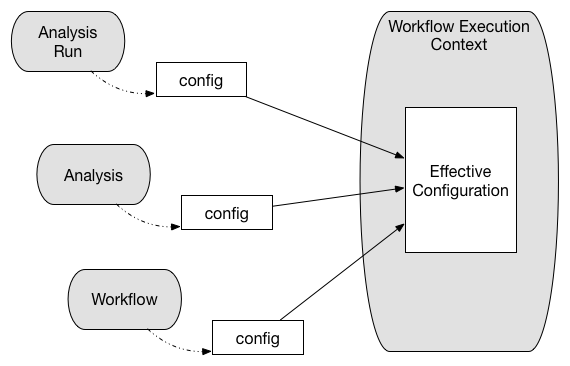
\includegraphics[width=\textwidth]{effective_configuration}
\centering
\caption {Tri-level configuration combines into an effective configuration at runtime.}
\label{fig:effective_configuration}
\end{figure}

The configuration facility is built into the \mintinline{python}{tracker} module, and is backed by a Run Tracking Database configuration table for persistence.

Because it is important for configuration to be both human-readable and machine-readable Butler uses the JSON format to encode configuration information. PostgreSQL, in turn, has native support for storage and deep querying of JSON values, thus making it an ideal choice for configuration persistence.

\subsubsection {Configuration Mechanism}

The mechanism by which configuration works is as follows:

A workflow author provides, together with their workflow definition, a JSON file that contains the most coarse-grained configurations related to the workflow. A system operator may customize some of these values before adding the workflow to a deployed version of Butler. Once the workflow is added to the system its accompanying configuration is persisted to the database.

A user who is running an analysis defines an analysis-level JSON file with more fine-grained configuration values. Algorithm parameters and flags are typical such values that vary from one analysis to the next. These are also persisted to the database along with the analysis definition.

As the analysis run corresponds to running a particular workflow in the context of a particular analysis on a particular sample, the user needs to generate a separate JSON configuration file for each sample in the analysis. These files will contain the most fine-grained configurations. Typical values at this level indicate where to locate the particular sample file for this run, and where to store the run results. An effective way to generate many JSON files for these runs is via a script.

When a workflow is executed on a particular sample, the JSON files corresponding to all three levels of configuration are retrieved from the database, merged, and parsed into a Python dictionary. This dictionary is then made available within the workflow execution context to guide workflow decision logic.

\subsection{Workflow Runtime Management}

Workflow Runtime Management encompasses the tools that are available to the user for the purpose of managing workflow execution. In Butler there are three separate mechanisms that exist for this purpose. These are:

\begin{itemize}
\item Butler CLI
\item Airflow CLI
\item Airflow Web UI
\end{itemize}

\subsubsection{Butler CLI}

The Butler CLI allows the user to create the various analysis management objects described in Section \ref{sec:analysis_tracker} via a Command Line Interface. The following commands are supported:

\paragraph{\mintinline{shell}{create-workflow}} - creates a new workflow and supports the following parameters:
\begin{description}
\item [-n, -\--workflow\_name] - The name of the workflow.
\item [-v, -\--workfow\_version] - The version of the workflow.
\item [-c, -\--config\_file\_location] - Path to the workflow configuration JSON file.
\end{description}

\paragraph{\mintinline{shell}{create-analysis}} - creates a new analysis and supports the following parameters:
\begin{description}
\item [-n, -\--analysis\_name] - The name of the analysis.
\item [-d, -\--analysis\_start\_date] - The starting date of the analysis.
\item [-c, -\--config\_file\_location] - Path to the analysis configuration JSON file.
\end{description}

\paragraph{\mintinline{shell}{launch-workflow}} - launches workflow execution and supports the following parameters:

\begin{description}
\item [-w, -\--workflow\_id] - ID of the workflow to launch.
\item [-a, -\--analysis\_id] - ID of the analysis to launch the workflow under.
\item [-c, -\--config\_location] - Path to a directory that contains analysis run configuration JSON files that will be launched. 
\end{description}

\paragraph{\mintinline{shell}{update-config}} - Update the configuration for a workflow or analysis.

\begin{description}
\item [-w, -\--workflow\_id] - ID of the workflow to update.
\item [-a, -\--analysis\_id] - ID of the analysis to update.
\item [-c, -\--config\_file\_location] - Path to the new config file.
\end{description}

\paragraph{\mintinline{shell}{get-run-count}} - Print to stdout the number of analysis runs for a particular analysis.

\begin{description}
\item [-a, -\--analysis\_id] - ID of the analysis to look up.
\item [-s, -\--run\_status] - Restrict the lookup to runs with a particular status
\end{description}

\subsubsection{Airflow CLI}

The Airflow CLI is part of the generic Airflow framework and provides a number of commands for workflow management. We describe several of the most useful ones below:

\paragraph{\mintinline{shell}{airflow}} - The main Airflow CLI command, with these supported sub-commands:

\begin{description}
\item [webserver] - Start an instance of the Airflow Web UI.
\item [scheduler] - Start an instance of the Airflow Scheduler.
\item [worker] - Start an instance of the Airflow Worker.
\item [flower] - Start an instance of the Airflow Flower, which is a monitoring tool.
\item [clear] - Clear the state of tasks that have failed or are stuck to allow them to be scheduled again.
\item [task\_state] - Print out the state of a task.
\item [initdb] - Initialize an empty Airflow database.
\item [resetdb] - Reset an Airflow database to the empty state.
\item [list\_dags] - List all of the available workflows.
\item [list\_tasks] - List all of the tasks for a particular workflow.
\end{description}

Butler provides wrappers for the \mintinline{shell}{webserver, scheduler, worker, and flower} commands so that they can be run as system services.

\subsubsection{Airflow Web UI}

The Airflow Web UI provides an interactive dashboard that allows the user to monitor the progress of workflows and workflow tasks, as well as taking some remedial actions when tasks run into trouble.

\begin{figure}[h]
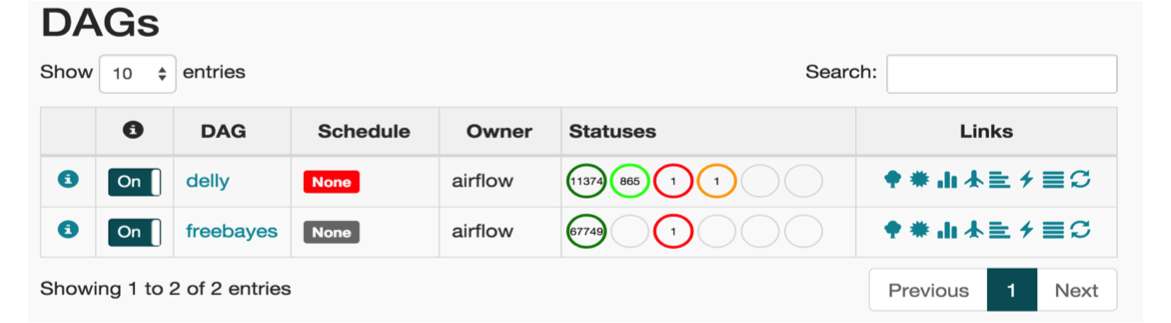
\includegraphics[width=\textwidth]{airflow_web_ui_main_page}
\centering
\caption {The main page of the Airflow Web UI}
\label{fig:airflow_web_ui_main_page}
\end{figure}

The main page of the Web UI features a listing of the available workflows, along with the breakdown of workflow tasks by status. In Figure \ref{fig:airflow_web_ui_main_page} we see two workflows - freebayes and delly. The delly workflow has 11374 completed tasks, 865 in-progress tasks, 1 failed task, and 1 task with a failed ancestor. The user can click on any of the task statuses to navigate to a task listing page that gives a comprehensive list of tasks along with their key attributes (see Figure \ref{fig:airflow_task_instances}.

\begin{figure}[h]
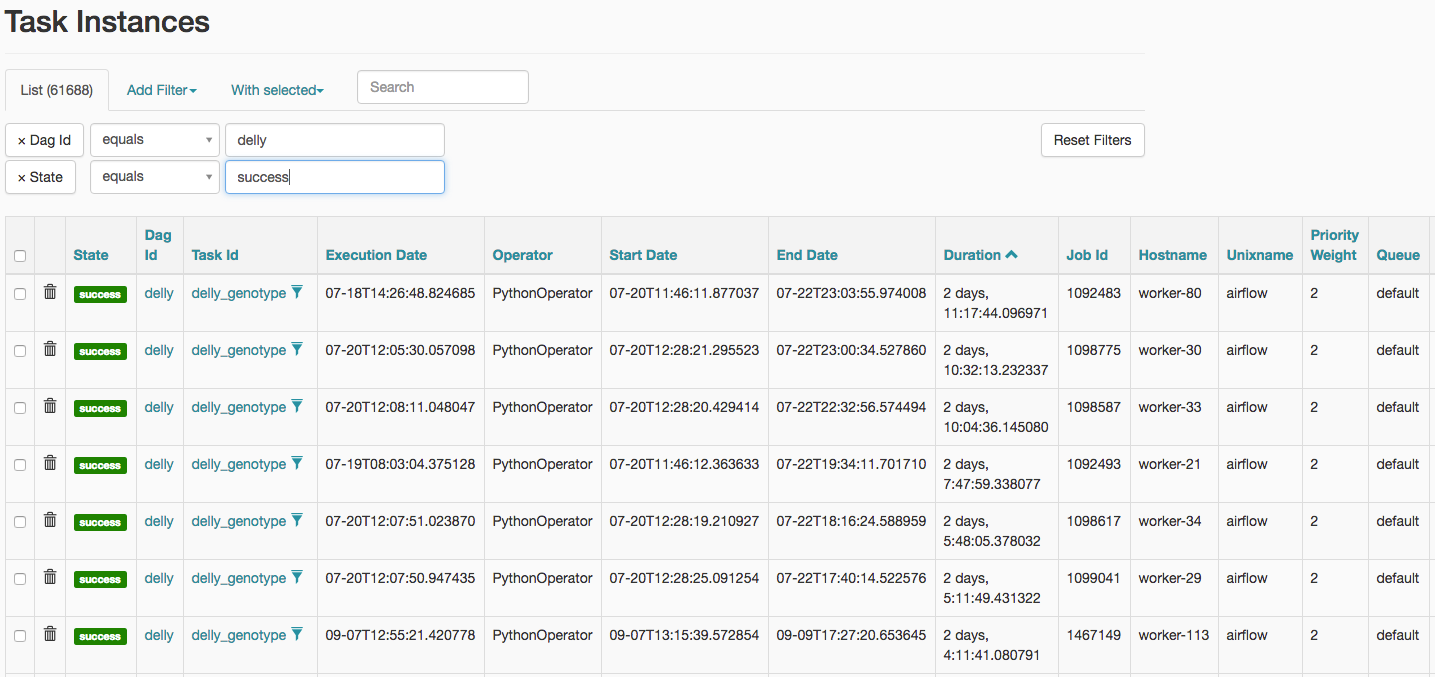
\includegraphics[width=\textwidth]{airflow_task_instances}
\centering
\caption {Listing of task instances for the freebayes workflow with status of "success".}
\label{fig:airflow_task_instances}
\end{figure}

Clicking on one of the task instances will bring up a graphical view of the workflow the task belongs to and allow the user to further investigate that workflow's execution (see Figure \ref{fig:airflow_workflow_details}). This view shows the status of all tasks in the corresponding workflow instance as well as providing links to various reports.

\begin{figure}[h]
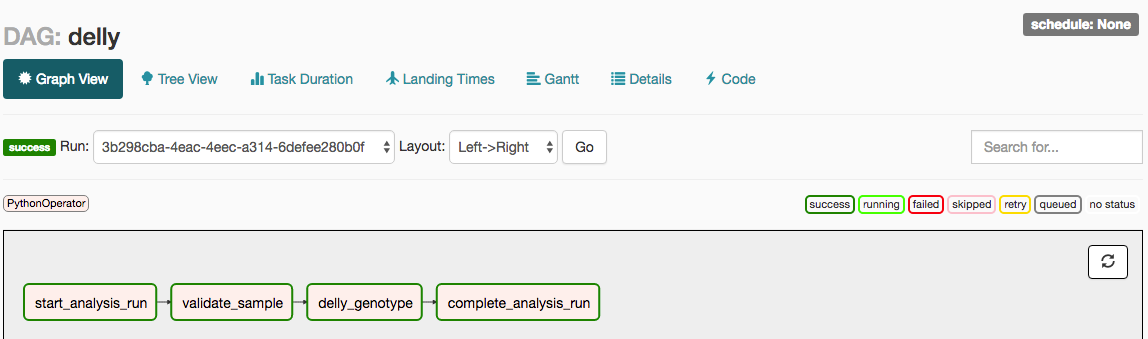
\includegraphics[width=\textwidth]{airflow_workflow_details}
\centering
\caption {Details of the execution of a delly workflow with ID 3b298cba-4eac-4eec-a314-6defee280b0f.}
\label{fig:airflow_workflow_details}
\end{figure}

When the user clicks on a particular task instance within the workflow execution a popup window allows them to take a number of actions, such as forcing the task to be run immediately, clearing the task state (for failed tasks) so that it can be run again, or marking the task as successfully completed (possibly with all upstream and downstream tasks). These options are depicted in Figure \ref{fig:airflow_task_actions}

\begin{figure}[h]
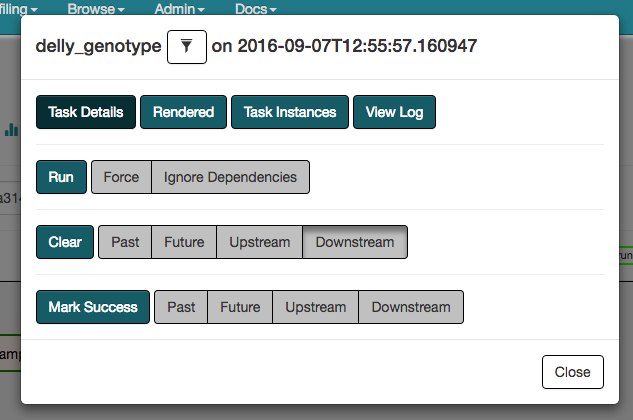
\includegraphics[scale=0.3]{airflow_task_actions}
\centering
\caption {A list of actions that can be taken on a workflow task via the Web UI.}
\label{fig:airflow_task_actions}
\end{figure}

\section{Operational Management}\label{sec:operational_management}

Managing large fleets of Virtual Machines as they perform data analysis at scale across multiple cloud computing environments is a major challenge due to the sheer number of possible scenarios that could lead to the system crashing, stalling, or otherwise falling out of control, with the negative impact on the end user in terms of project costs and timeline increasing with the scale of the computation being undertaken. The tools available to the user to detect and deal with these issues thus form a key component of a comprehensive analysis framework and set Butler apart from other frameworks in this space.

In general, the Operational Management tools fall into three categories, those that collect observations about the state of each component in the system at runtime, those that aggregate this data and present it to the user in the form of queryable databases and management reports, and those that take automated remedial steps to resolve identified issues. Furthermore, as specified in the requirements of Section \ref{sec:troubleshooting} we delineate two major sources of data that is indicative of system state - System Metrics, and Server Logs. While metrics provide more of a coarse-grained view of the overall health of a particular Virtual Machine, server logs can give much more of a fine-grained view of the underlying system at an application level, and down to individual lines of code that are running at any given time. Butler has dedicated components for the collection and management of these data sets and we describe these next.

\begin{figure}[h]
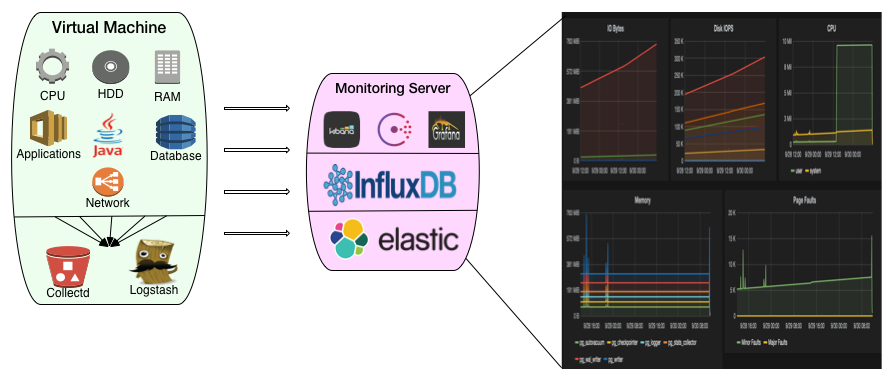
\includegraphics[width=\textwidth]{monitoring_server}
\centering
\caption {Metric monitoring system components}
\label{fig:monitoring_server}
\end{figure}

\subsection{Monitoring Metric Collection}

The overall health of any VM in a cloud computing cluster can be evaluated and ascertained with respect to a set of key metrics that are observable at runtime. Some metrics are general enough that they apply to all Virtual Machines, these include measurements of CPU utilization, RAM, Disk, and Network usage. Other metrics are more specific to the role that the VM is playing within the cluster. A Database Server will benefit from having the number of open DB connections, transaction rate, rollback rate, and average query runtime monitored. Other entities such as Web Servers and Queues have their own unique metrics of interest.

Each VM runs a metric collection daemon called \mintinline{shell}{telegraf}\autocite{telegraf} which is an Open Source package that is able to make periodic measurements of a large number of system metrics and ship them off to a centralized Metrics Store. The definition for which metrics are collected is specified in a special configuration file. An example of such configuration is demonstrated in Listing \ref{lst:telegraf_config}. This listing provides examples of the setup for generic metrics like CPU, and memory, as well as for more special metrics, like those collected for PostgreSQL databases.

Because we are interested in observing not only the metrics as they are measured in the present, but also the dynamics of how metric values change over time, we need a mechanism for persisting the metrics values. For this purpose the Monitoring Server component of Butler ships with an instance of a database product called InfluxDB\autocite{InfluxDB} which is an Open Source database system that is optimized for recording time series data. The configuration for the \mintinline{shell}{influxdb} output plugin in Listing \ref{lst:telegraf_config} demonstrates how InfluxDB server URL is provided to Telegraf to enable metrics persistence in this centralized data store.

InfluxDB is a scalable database system that can operate in a distributed manner as a Raft\autocite{ongaro2014search} cluster. Data is written into shards based on a data retention policy. The underlying engine stores the data as a Time-Structured Merge Tree (TSM) which is a customization of the Log-Structured Merge-Tree\autocite{o1996log} data structure. To the end user the data is organized as a collection of \mintinline{shell}{points}. Each point has a \mintinline{shell}{timestamp}, belongs to a \mintinline{shell}{measurement}, and records a set of \mintinline{shell}{tag_values} that correspond to a set of \mintinline{shell}{tag_keys}. A particular \mintinline{shell}{measurement} coupled with a retention policy then forms a \mintinline{shell}{series}.

As an example, when tracking RAM, our \mintinline{shell}{measurement} is called \mintinline{shell}{memory_value}. The set of \mintinline{shell}{tag_keys} is:

\begin{itemize}
\item host
\item type
\item type\_instance
\end{itemize}

An example set of \mintinline{shell}{tag_values} might be:

\begin{itemize}
\item worker-145
\item memory
\item free
\end{itemize}

The actual \mintinline{shell}{points} corresponding to this combination of \mintinline{shell}{tag_values} and collected over the period of 1 minute might look as follows:

\begin{figure}[h]
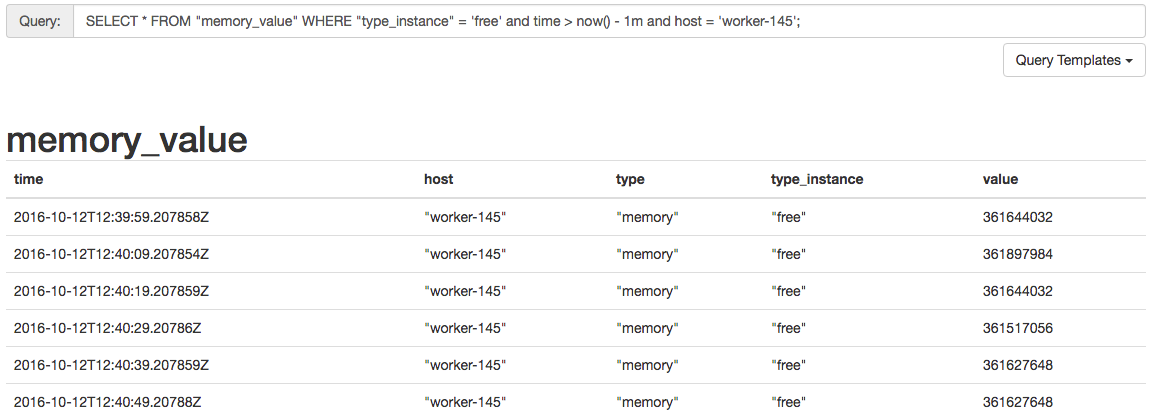
\includegraphics[width=\textwidth]{influxdb_example_query}
\centering
\caption {InfluxDB query results showing free memory on host worker-145 collected in a 1 minute time window.}
\label{fig:influxdb_example_query}
\end{figure}

As can be seen in Figure \ref{fig:influxdb_example_query}, data is queried via an SQL-like dialect which is accessible via a Web UI or via a REST\autocite[Chapter~5]{fielding2000architectural} API.

\subsection{Monitoring Visualization}

The metrics collection system is collecting 50 different metrics per host on average, sampled at intervals of 10 seconds. Given a cluster of 200 Virtual Machines the monitoring system collects and stores 86,400,000 data points in a 24 hour time period. This volume of data is quite difficult for the user to comprehend and make use of, and Butler provides visualization tools to enable the display of aggregate statistics based on the monitoring data using a Graphical User Interface. The main goal of the visualizations is to give the user an overview of the trends observed within the compute cluster with respect to a set of representative performance metrics, and to alert the user to any conditions that threaten the health of Virtual Machines and the scientific analyses they run.

Visualization of performance metrics data is accomplished in Butler using an Open Source framework called Grafana\autocite{Grafana.net}. This framework provides a Web Interface that is able to connect to an instance of an InfluxDB database, issue queries and render the query results as dashboard of various graph styles, including line graphs, bar graphs, pie charts, and others. Reports generated by Grafana support parametrization of values as well as drill-through.

Butler ships with a number of pre-built reports and supports the addition of custom reports if necessary.

In general, Grafana is a website that the user logs onto to either author or view reports. When authoring reports the user needs to define a Data Source to connect the reports with data. In the case of Butler, the Data Source is connecting to the InfluxDB metrics database using the InfluxDB REST API.

\begin{figure}[h]
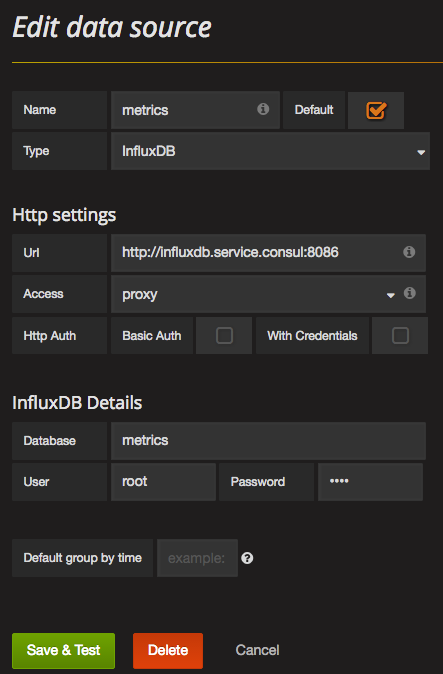
\includegraphics[scale=0.4]{grafana_data_source}
\centering
\caption {InfluxDB Data Source creation for Grafana.}
\label{fig:grafana_data_source}
\end{figure}

Once a connection to the Data Source is established the user can begin building dashboards. Dashboards are generally laid out in a grid-like fashion as a series of panels that are arranged into rows and columns. Each panel contains a graph. Data is fed into the graph by means of an InfluxDB Query Language query, possibly with additional parameters specified by the report.  In addition to the query itself, the user can customize the axes, legend, and other attributes of each graph. Once the report is ready it can be exported into a JSON format and checked into a source code repository so that it can persist if the VM hosting the Grafana instance needs to be recreated.

\begin{figure}[h]
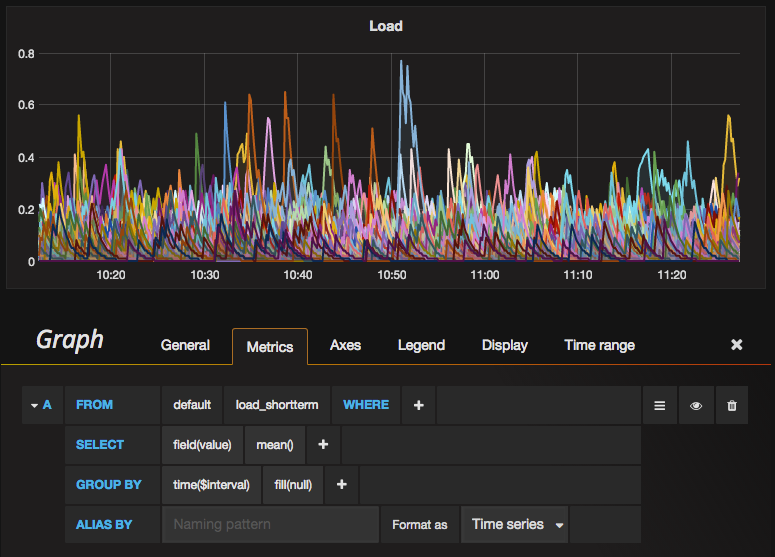
\includegraphics[width=\textwidth]{grafana_report_editing}
\centering
\caption {Editing a Grafana dashboard panel.}
\label{fig:grafana_report_editing}
\end{figure}

Butler comes with a set of basic dashboards defined out-of-the-box that will aid the user in monitoring of overall system health. The most important dasbhoards are:

\begin{description}
\item [Cluster Overview] - Gives a high level overview of the health of the entire cluster, tracking metrics such as load (blended health metric), CPU utilization, Memory, Disk IOPS, Network Packet Rate, Disk Read/Write Rates, and Disk Space
\item [Salt Master] - Detailed monitoring of the Salt Master VM, including CPU, Memory, Network Packet Rate, Disk Read/Write Rates, Disk IOPS, and Disk Space.
\item [Database Server] - Detailed monitoring of the Database Server VM, including DB-specific metrics such as - DB Connections, Number of Transactions, Number of Queries, Number of Query Plans, Number of Rows, DB Size on Disk, as well as the general VM health metrics.
\end{description}

\begin{figure}[h]
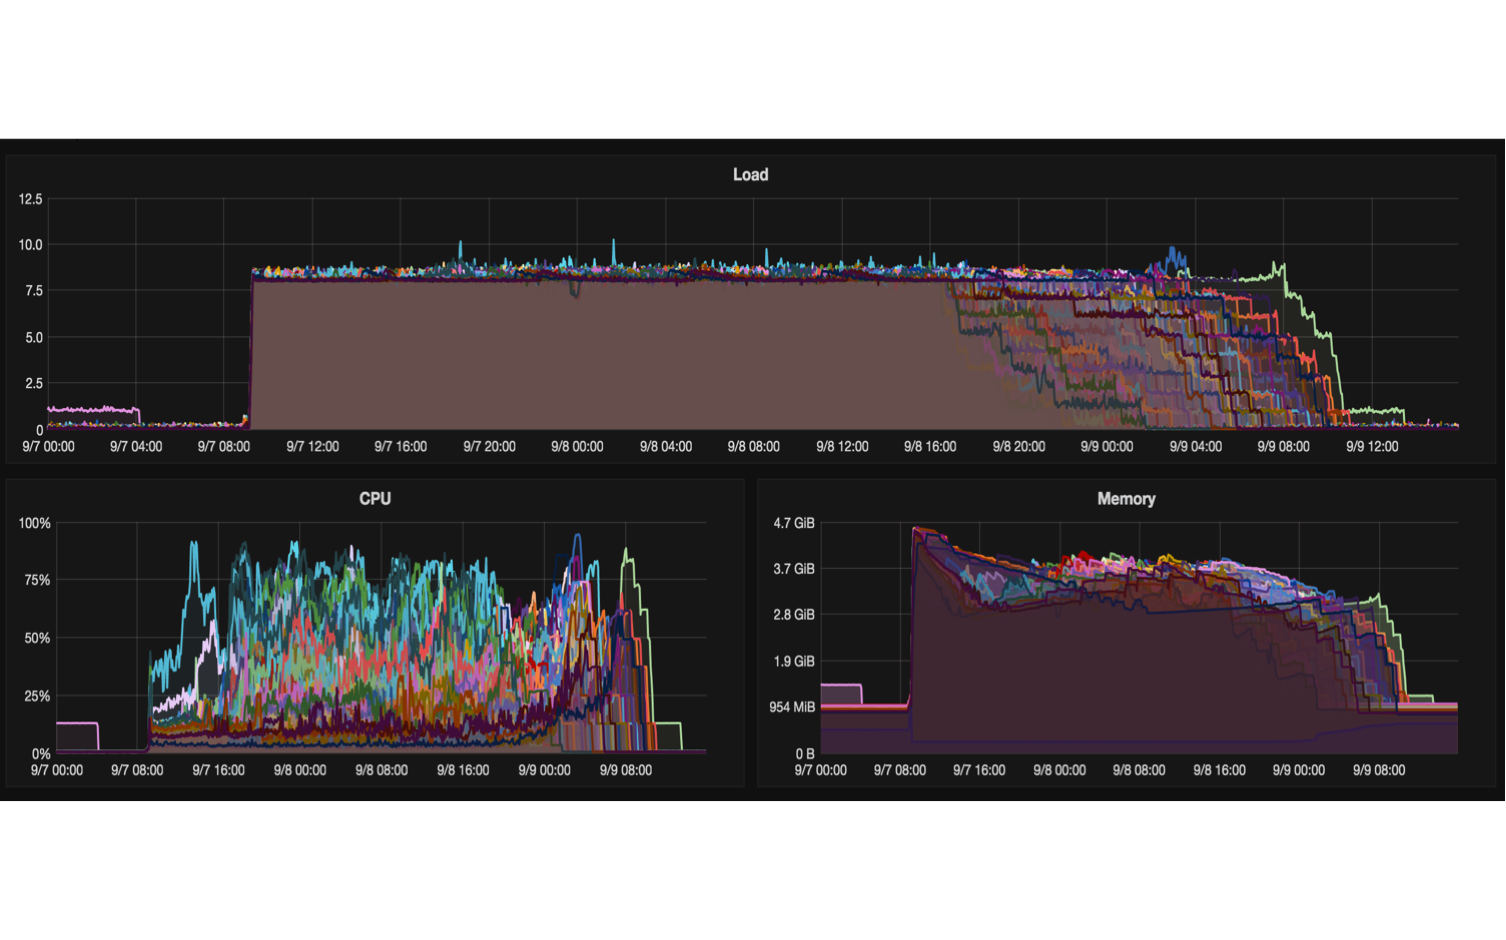
\includegraphics[width=\textwidth]{grafana_cluster_overview_normal}
\centering
\caption {Cluster Overview dashboard during normal operation.}
\label{fig:grafana_cluster_overview_normal}
\end{figure}

In practice the Cluster Overview dashboard is the most consistently useful report because it provides an at-a-glance view of the health of the entire cluster. Figure \ref{fig:grafana_cluster_overview_normal} demonstrates a typical scenario of cluster usage during normal operation. It is evident that the cluster starts off without any appreciable load, once a set of workflows is scheduled system load increases across the entire cluster and remain stable until, towards the end of the execution, machines start running out of work, and load of the system gradually decreases. Throughout the execution the memory profile is relatively stable and consistent across the machines in the cluster. Although the CPU profile appears spiky, this is the natural CPU utilization profile for the particular set of workflows that were executing at the time the image was captured.

\begin{figure}[h]
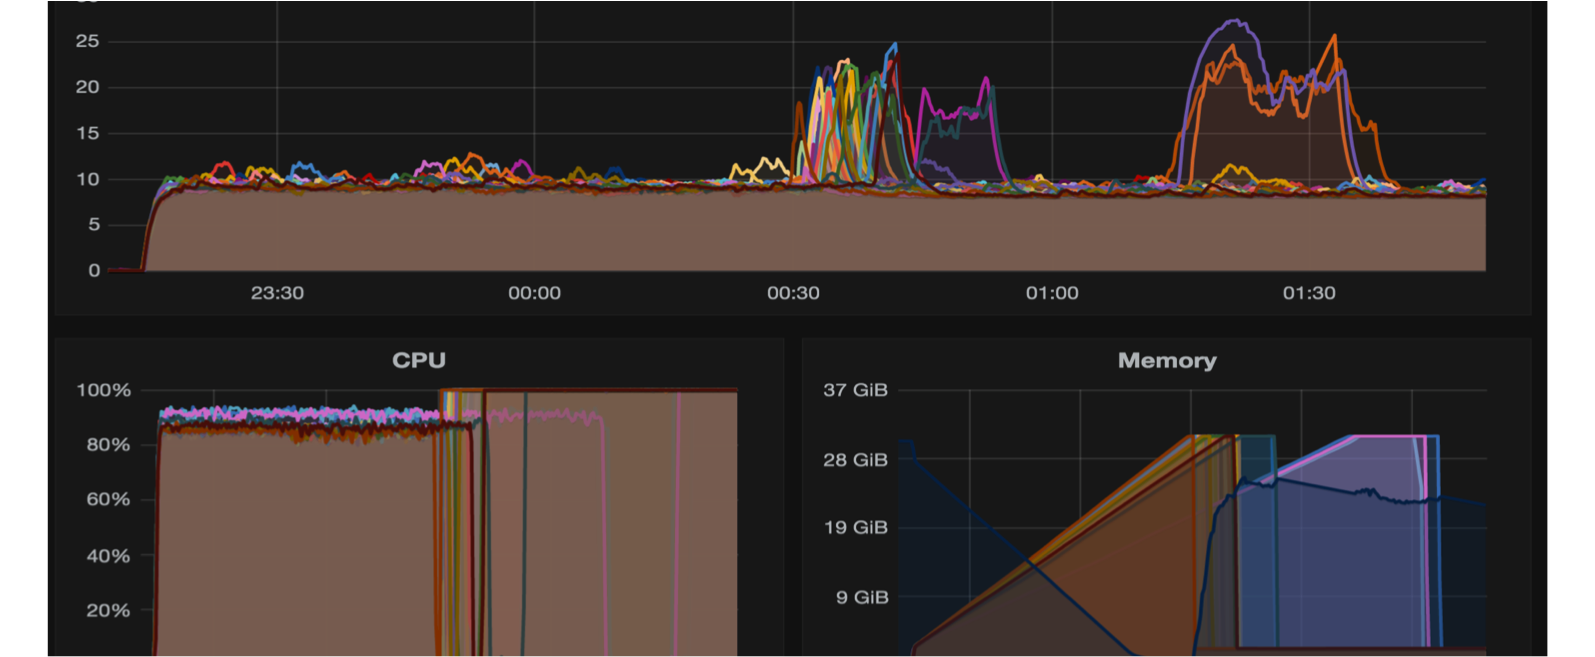
\includegraphics[width=\textwidth]{grafana_cluster_overview_issue}
\centering
\caption {Cluster Overview dashboard demonstrating a cluster-wide issue.}
\label{fig:grafana_cluster_overview_issue}
\end{figure} 

Figure \ref{fig:grafana_cluster_overview_issue}, on the other hand, demonstrates an example of how a cluster-wide issue can be identified via the Cluster Overview dashboard. Here we see a similar profile at the beginning of workflow execution, where the jobs get kicked off and load is stable, but at around 00:30 we start seeing uncharacteristic spikes in system load, with sporadic doubling of load metric values. Furthermore, the CPU utilization appears to drop to 0 at the same time, and the memory profile is highly irregular. This pattern signifies to the user that an issue is affecting the cluster during this particular time, and further investigation is needed. With that knowledge, the user can use other reports to try to pinpoint the source of the issue, or it may be necessary to directly log on to the affected VM hosts to investigate further.

Because collectd allows collecting metrics from a particular named process, and because Grafana allows the creation of new dashboards on the fly, it is common and convenient for the user to develop a set of custom dashboards that are targeted towards the specific workflows that they are running, thus providing much more fine-grained visibility into the runtime behaviour of the system. Together with the built in reports these custom dashboards provide a powerful and flexible set of capabilities for successful operational management of the Butler system. 

\subsection{Server Log Collection and Visualization} 
\label{sec:design_log_collection}

Almost every application that runs on a computer is generating some sort of log file. On Unix-based environments most system-level applications will write to a common log known as syslog. But many other applications will write their own custom logs to their own specific locations. Messages written to a log file typically run the gamut from INFO statements that mark the normal operation of an application, all the way to ERROR which signify error conditions. Thus, a log file, potentially provides a wealth of information about both normal operation and system issues as they occur, and is typically one of the most reliable sources for information on application crashes. On the other hand, when operating a complex distributed system, such as a large scale workflow execution framework which runs on hundreds of Virtual Machines, the number and size of logs can become overwhelming to the point of ceasing to remain useful.  

Because of the potentially extremely high value of the information contained in server logs, we deploy a system of log harvesting and centralized storage that enables the Virtual Machines that are part of Butler to parse the logs that are being generated locally for interesting events, and send those events to a centralized search index which is amenable to efficient querying and visualization. Although the three tools that we use to solve the centralized logging problem have been developed independently, they have since been acquired by a single company Elasticsearch BV. These three tools form what is known as the ELK stack - Elasticsearch\autocite{Elasticsearch}, Logstash\autocite{Logstash}, and Kibana\autocite{Kibana}.

Each Virtual Machine in the cluster runs a log shipper - Filebeat. It is responsible for finding, harvesting, and locally aggregating logs.

\begin{figure}[h]
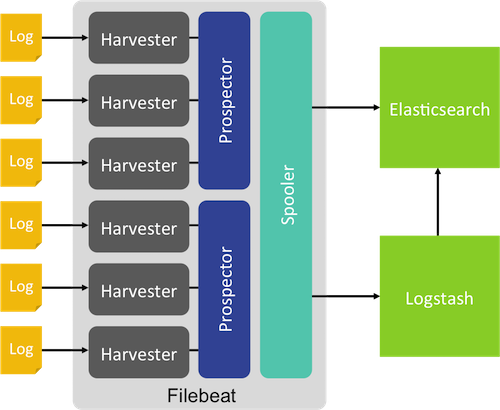
\includegraphics[scale=1]{filebeat}
\centering
\caption {Filebeat Architecture (taken from https://www.elastic.co).}
\label{fig:filebeat}
\end{figure}

As shown in Figure \ref{fig:filebeat}, Filebeat consits of a set of Prospectors (see Listing \ref{lst:filebeat_prospectors})which monitor and search log directories specified in the Filebeat configuration file. Corresponding to each log file that is found by Prospectors a separate Harvester is started which is responsible for ingesting the log file and sending the information to a Spooler. The Spooler aggregates information sent from Harvesters and forwards it onto Logstash for further parsing.

Logstash runs on a separate centralized server and is responsible for parsing the logs forwarded from Filebeat and sending the parsed information on to the Elasticsearch index. The parsing is accomplished via 3 plugins - Input Plugin, Filter Plugin, and Output Plugin (see Figure \ref{fig:logstash_pipeline}). All three plugins are configured via the logstash configuration file.

\begin{figure}[h]
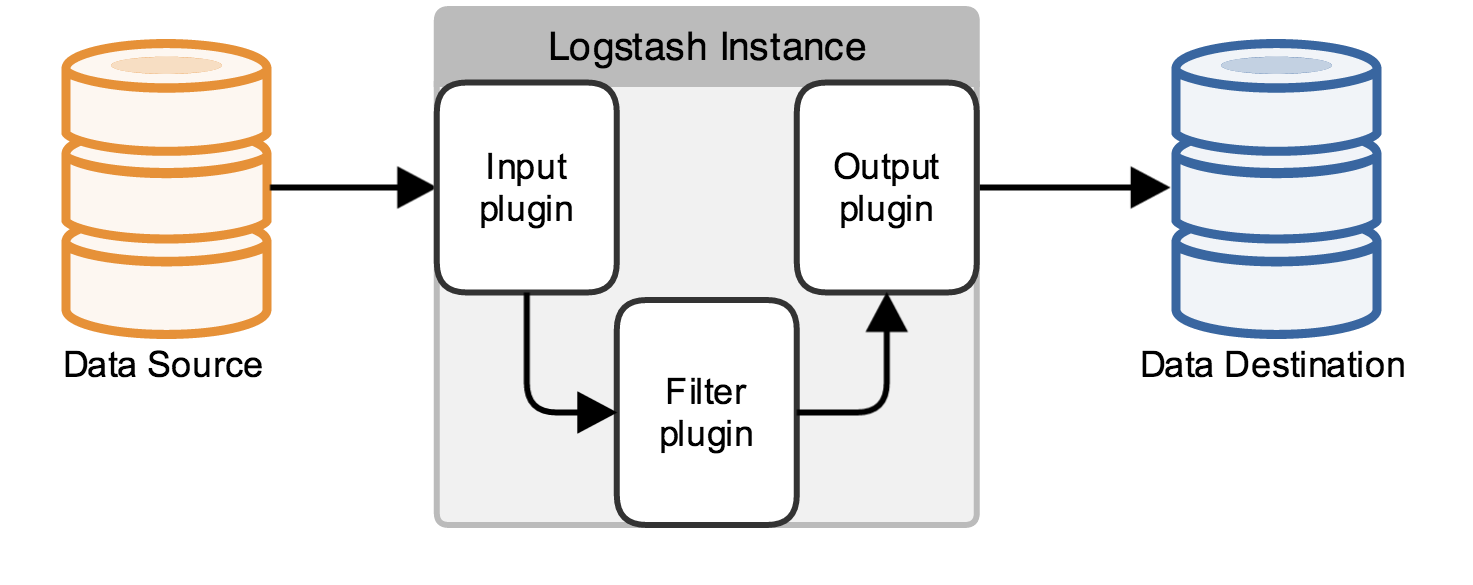
\includegraphics[scale=0.2]{logstash_pipeline}
\centering
\caption {A Logstash processing pipeline (taken from https://www.elastic.co).}
\label{fig:logstash_pipeline}
\end{figure}

The Input Plugin specifies where to listen to input data from. In the case of Butler we are expecting data to arrive in Filebeat format on port 5044.

The Filter plugin specifies how to parse the log file i.e. which messages from each type of log file we are interested in. The interesting messages are identified using a series of regular expressions known as grok patterns. 

The output plugin then specifies how to pass the filtered messages on to the Elasticsearch engine for indexing.

Elasticsearch is a general purpose scalable text indexing and search engine that supports clustering and sharding of data. Given its longterm use as a storage engine for log data and its scalability it is a great fit for Butler's log storage needs. Elasticsearch works by storing JSON formatted documents (in this case log messages) into an searchable index. 

Just as it is difficult to grasp and analyze performance metrics due to the number of data-points generated, it is as difficult to grasp log messages from a large cluster. We utilize a similar set of visualization tools to the ones we used for metrics, to solve this problem for server logs within Butler. The Kibana dashboarding framework allows us to create graphical dashboards that visualize log events of interest, as well as providing a web-based query interface to the Elasticsearch log messages index. Figure \ref{fig:kibana_pgsql_dashboard} shows a dashboard used in Butler for monitoring the Database Server.

\begin{figure}[h]
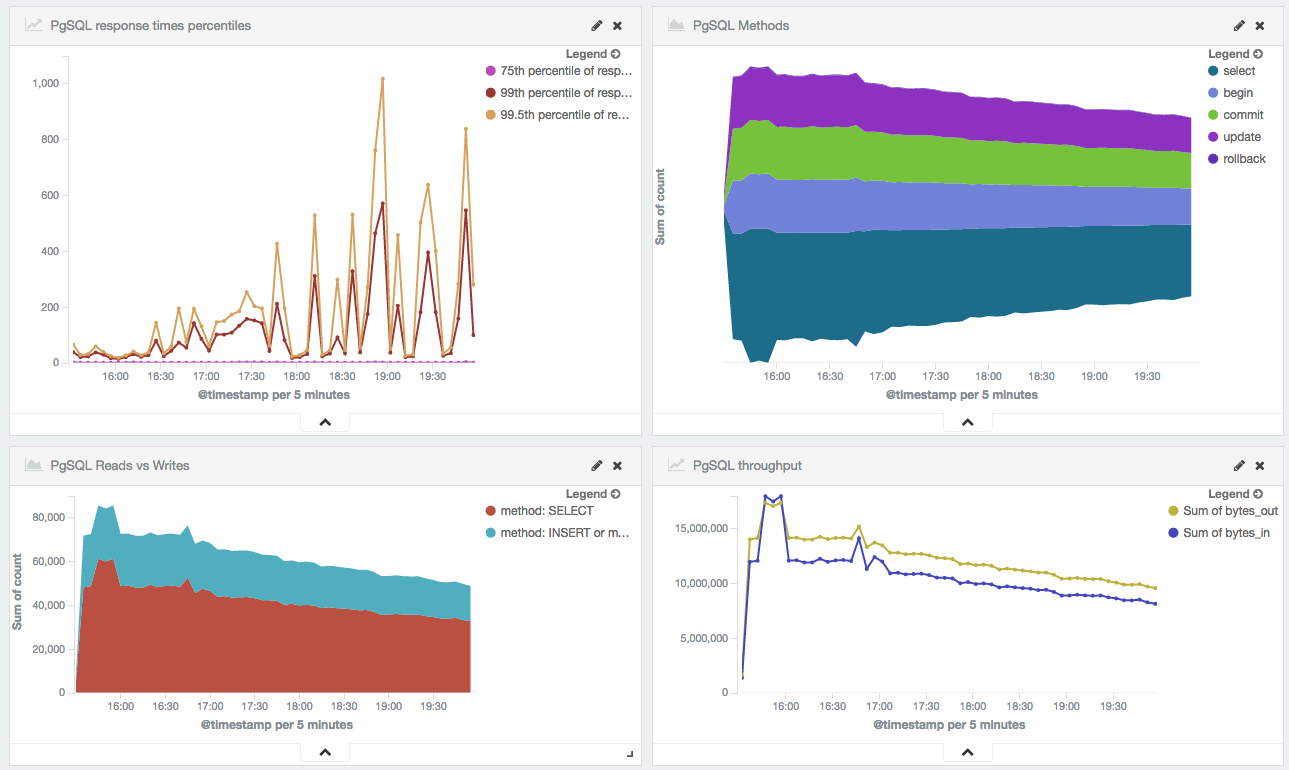
\includegraphics[width=\textwidth]{kibana_pgsql_dashboard}
\centering
\caption {Kibana dashboard for PostgreSQL monitoring.}
\label{fig:kibana_pgsql_dashboard}
\end{figure}
 
\subsection{Self-Healing}
\label{sec:self_healing}

The self-healing system within Butler builds on top of the metrics collection system to deliver features specified in Section \ref{sec:self_healing_req} of the requirements. Specifically, it aims to provide a comprehensive set of tools for detecting operational anomalies at multiple levels of the system and taking automated remedial steps to fix these anomalies in order to minimize their effects. Figure \ref{fig:butler_self_healing} demonstrates the components of this system.

\begin{figure}[h]
    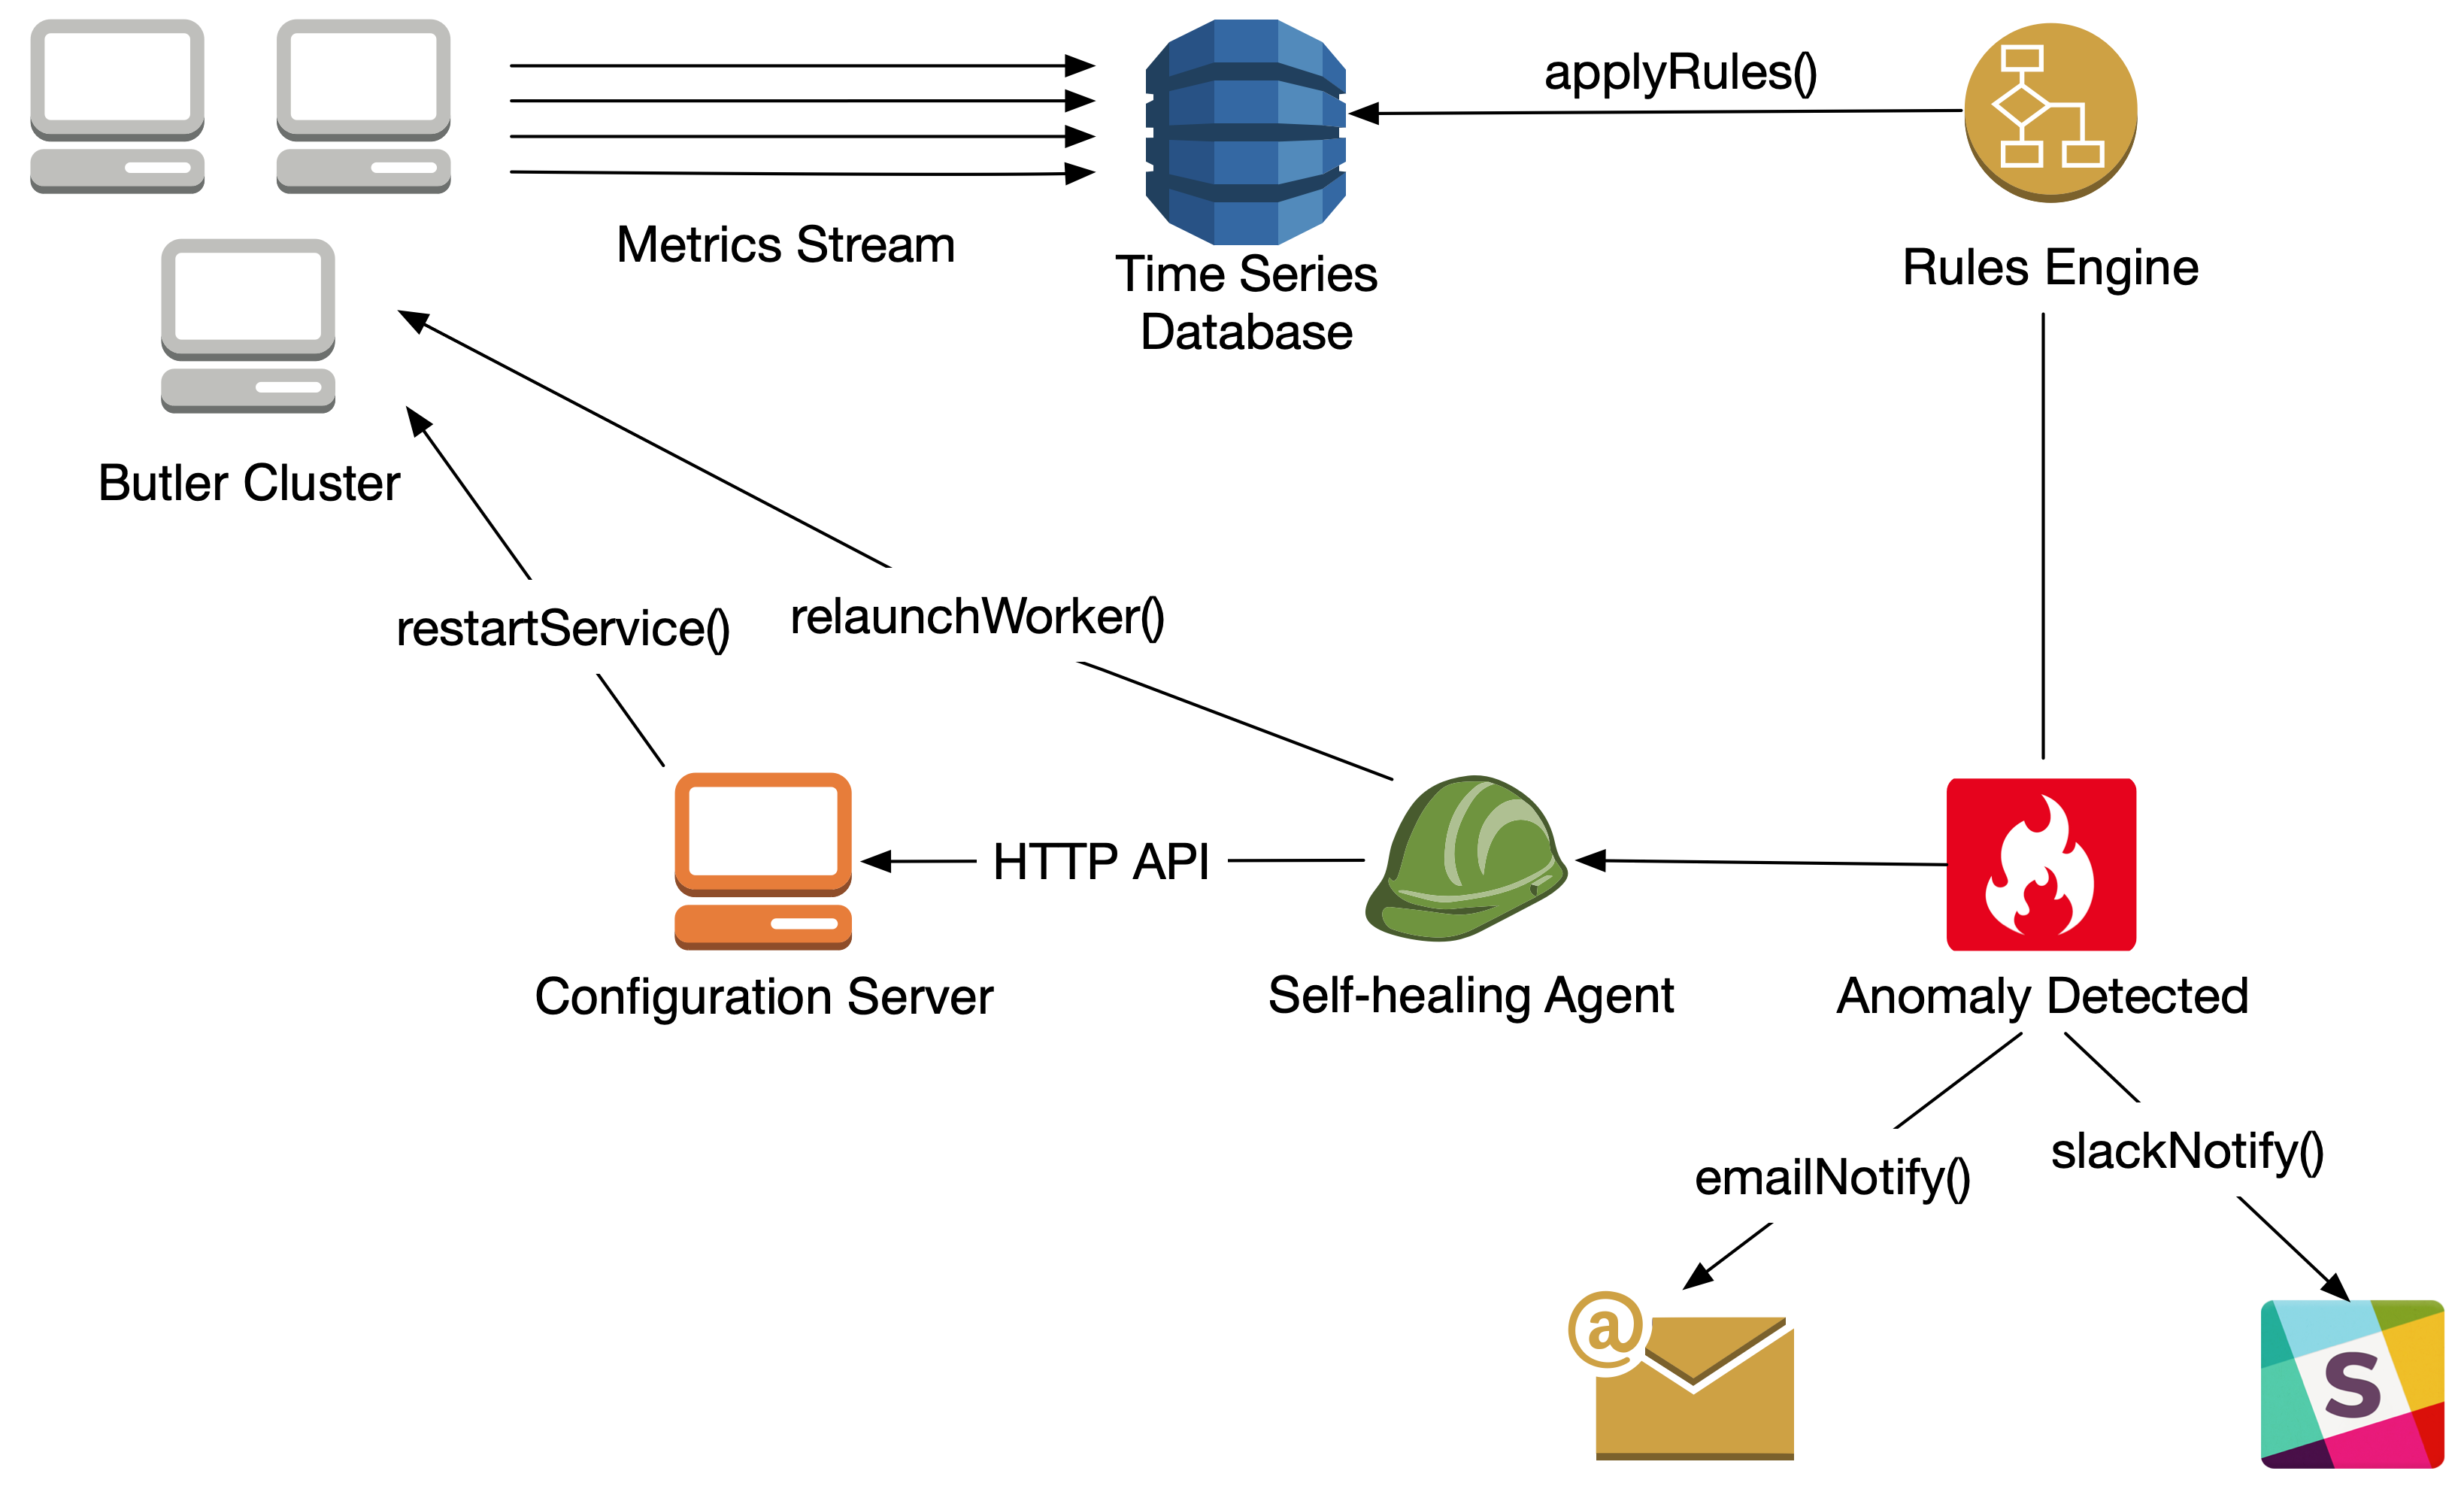
\includegraphics[width=\textwidth]{butler_self_healing}
    \centering
    \caption {The Butler self-healing system.}
    \label{fig:butler_self_healing}
\end{figure}

\subsubsection{Capturing Metrics}

The input to the self-healing system is the set of metrics that is collected from all hosts into InfluxDB via telegraf. In order to facilitate the detection of anomalies at infrastructure, service, and payload levels it is necessary to collect several types of metrics. 

Infrastructure-level issues are a wide class off issues that can represent the failure or entering into a bad state of individual components of the VM or the entire VM. Detecting these relies on capturing of a variety of basic metrics such as CPU, memory, disk, network, and others. Failure of the entire VM can be detected by the complete absence of a metrics signal from the affected machine. In practice, Butler uses the lack of updates to the \mintinline{shell}{uptime} metrics as a signal that the machine has gone offline.

Tracking of individual services is facilitated by monitoring their respective processes. There are several possibilities for doing this offered by telegraf with its \mintinline{shell}{procstat} input plugin and these are used to capture the necessary processes in Butler. See listing \ref{lst:procstat_plugin} for the variety of ways to capture a process employed within Butler. Here, a process can be targeted by capturing the name of its executable, its PID file, a grep pattern on the process name, or the user that owns the process. Capturing the process in this way will generate a set of process-specific metrics that record the process's CPU usage, memory, context switches, and others that can be used in detecting and diagnosing issues.  

\captionof{listing}{Butler Analysis configuration for VCF filtering.\label{lst:procstat_plugin}}
\begin{minted}
[
breaklines=true,
breakanywhere=true,
fontsize=\footnotesize,
linenos,
frame=lines,
framesep=2mm,
baselinestretch=1.2
]
{shell}
[inputs.procstat]]
exe = "grafana-server"

[[inputs.procstat]]
pid_file = "/var/run/salt-api.pid"

[[inputs.procstat]]
pattern = ".*airflow scheduler.*"

[[inputs.procstat]]
user = "airflow"
\end{minted}

Tracking detailed metrics at the payload level beyond what is offered by procstat is, by definition, not possible to do in a completely generic fashion because every user of the framework will potentially run their own custom payloads that need to be individually instrumented with metrics. In usage scenarios where the payload is of a particularly experimental nature (such as scientific algorithms that are in early stages of development), or the analysis is performed at a large scale where the runtime is expected to be in months, and there is access to the underlying tools' source code, it may be desirable to add metrics emitting code within the individual tools that are run by the Butler framework. This is supported in Butler via the popular \mintinline{shell}{statsd}\autocite{statsd} package which has client libraries in every major programming language and allows any software to capture and emit several kinds of custom metrics in a format that is understood by a wider variety of metrics collection back-ends, including InfluxDB. The metric types that can be captured are:

\begin{description}
    \item [Counter] - A simple counter that allows arbitrarily incrementing and decrementing a value.
    \item [Timer] - A metric that measures passage of time.
    \item [Gauge] - A metric that emits a measurement of an arbitrary value.
    \item [Set] - A metric that counts unique occurrences of an event.
\end{description}

Using the basic metric types above one can construct metrics capturing schemes of arbitrary complexity that subsequently feed into the self-healing capabilities of the framework.

\subsubsection{Defining Anomalous Operating Conditions}

In order to perform self-healing the Butler framework needs to be able to detect when anomalous conditions occur. This is most easily accomplished via a rules-based system over the universe of metrics where each rule is a predicate of the form:

\begin{equation}\label{eq:1}
    f(\vec{\mathbf{M_n}})\quad op \quad C
\end{equation}

given: 

$M = \{M_t; t \in T\}$ - a metric time series\\
$\vec{\mathbf{M_n}} = [M_{t-n+1} \quad M_{t-n+2} \quad ... \quad M_t]$ - a vector of n most recent observations of $M$\\
$f\colon \mathbb{R^{n}} \mapsto \mathbb{R}$ - a function of $\vec{\mathbf{M_n}}$ that typically computes a summary statistic over a moving window of the most recent n data points, such as mean, min, max, etc.\\
$op \in \{>,<, >=, <=, ==, !=\}$ - is a comparison operator\\
$C \in R$ - is an arbitrary constant\\

Thus, each rule continuously (discretized by metric sampling frequency) computes a summary statistic over a sample of $n$ most recent observations of metric of interest $M$, and compares it to a threshold value $C$, firing off an event when the comparison specified in $op$ succeeds. The full collection of rules then constitutes a full specification of the set of anomalous conditions for which automated action can be taken.

We implement this rule-based system in Butler by leveraging an open-source product called Kapacitor\autocite{kapacitor} which provides a rule definition and execution environment that integrates well with our metrics data store InfluxDB and provides a wide range of options for event handling, including completely custom event handlers, which we make use of to implement the automated healing functionality in Butler. Kapacitor rule definitions make use of a Domain Specific Language (DSL) called TICKscript to implement the specification of rule predicates described in \ref{eq:1}.

TICKscript makes use of the concept of nodes and pipelines to organize rules as Directed Acyclic Graphs (DAGs) where processing flows forwards in a single direction, and never backwards. Each node describes a particular data processing stage, and the pipeline is a chain of nodes. Each invocation of a rule represents a particular path through the graph.

In listing \ref{lst:cpu_value_tick} we see an example of a TICKscript used in Butler to keep track of the CPU allocation on each host and send results to a log file. Key threshold levels are specified at the top of the script as well as the look-back period and evaluation frequency. A query for fetching appropriate data is specified and stored in the \mintinline{shell}{data} variable as a stream. Here we access the \mintinline{shell}{metrics} database (of our centralized InfluxDB data store), and we are interested in the \mintinline{shell}{cpu_value} measurement, expressed as a percentage. The actual metric measures the idle CPU percentage, and we are interested in the used CPU percentage, so we subtract the metric value from 100, and compute the mean value over our selection window giving it an alias name of \mintinline{shell}{stat} that we can refer to later. 

With the data appropriately selected we can turn our attention to specifying appropriate comparisons to the thresholds that had earlier been established, and defining event triggers and handling logic. In addition to the already existing mean value we use the built-in \mintinline{shell}{sigma} function to calculate the distance, in standard deviations, from the mean of the current \mintinline{shell}{stat} value, giving it an alias \mintinline{shell}{sigma} as we are interested in capturing and alerting not only on high absolute CPU utilization levels but also high variance within the metric of interest. Each rule can trigger at three levels of severity - info, warning, and critical and we specify a separate threshold for each level. Thus, the CPU rule is triggered at a critical level when average CPU utilization over the last 10 seconds is greater than 90\%, or when the observed CPU utilization is greater than 3.5 standard deviations away from the mean CPU utilization. Other thresholds are set similarly. In this particular example we are interested in collecting the instances when rules are triggered into a simple log file, thus we specify a path to such a log file as part of the alert definition.

A key mode of failure for the system is when a critical service fails or an entire virtual machine becomes unresponsive and unreachable. In order to capture these conditions we make use of a special type of rule within \mintinline{shell}{kapacitor} called a \emph{deadman}. This type of rule is triggered when no signal is received for a specific metric for a predefined period of time. In Listing \ref{lst:host_deadman_tick} we provide an example of a TICKscript that detects the deadman condition for an entire VM. This script uses a higher level of parametrization than the CPU utilization script of Listing \ref{lst:cpu_value_tick} where most of the parameters are specified as variables at the top of the script and the script structure is encoded below. The metric measurement that we base the rule on is called \mintinline{shell}{system} and it tracks low-level stats such as uptime for a VM. The data selection section of the script selects values from the \mintinline{shell}{system} measurement grouped by individual host that they originate from.

The rule is triggered when no data is received for the given metric via the \mintinline{shell}{deadman(threshold, period)} node. In this case, when the rule is triggered there are several handlers that are registered to handle the resulting event. The first handler uses Slack API\autocite{slack} to post a notification message to the \emph{\#embassyalerts} Slack channel using a predefined message template with key information about the outage, such as in Figure \ref{fig:self_healing_slack}. The type of message changes depending on whether the rule condition has triggered or returned back to normal.

\begin{figure}[h]
    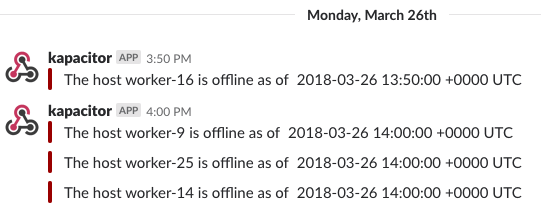
\includegraphics[scale=0.7]{self_healing_slack}
    \centering
    \caption {Self-healing alerts sent to a Slack channel.}
    \label{fig:self_healing_slack}
\end{figure} 

The second handler invokes the actual Butler Self-Healing Agent to destroy the host that has become defunct and to launch a new VM to replace it. The details of the agent are provided in the next section. The third handler for this event actually generates a new metric that keeps track of rules that have been triggered and stores the metric in a separate measurement in InfluxDB. Since we want to have comprehensive information about when error conditions occur the \mintinline{shell}{alerts} measurement gives us a system of record for these events.

\begin{figure}[h]
    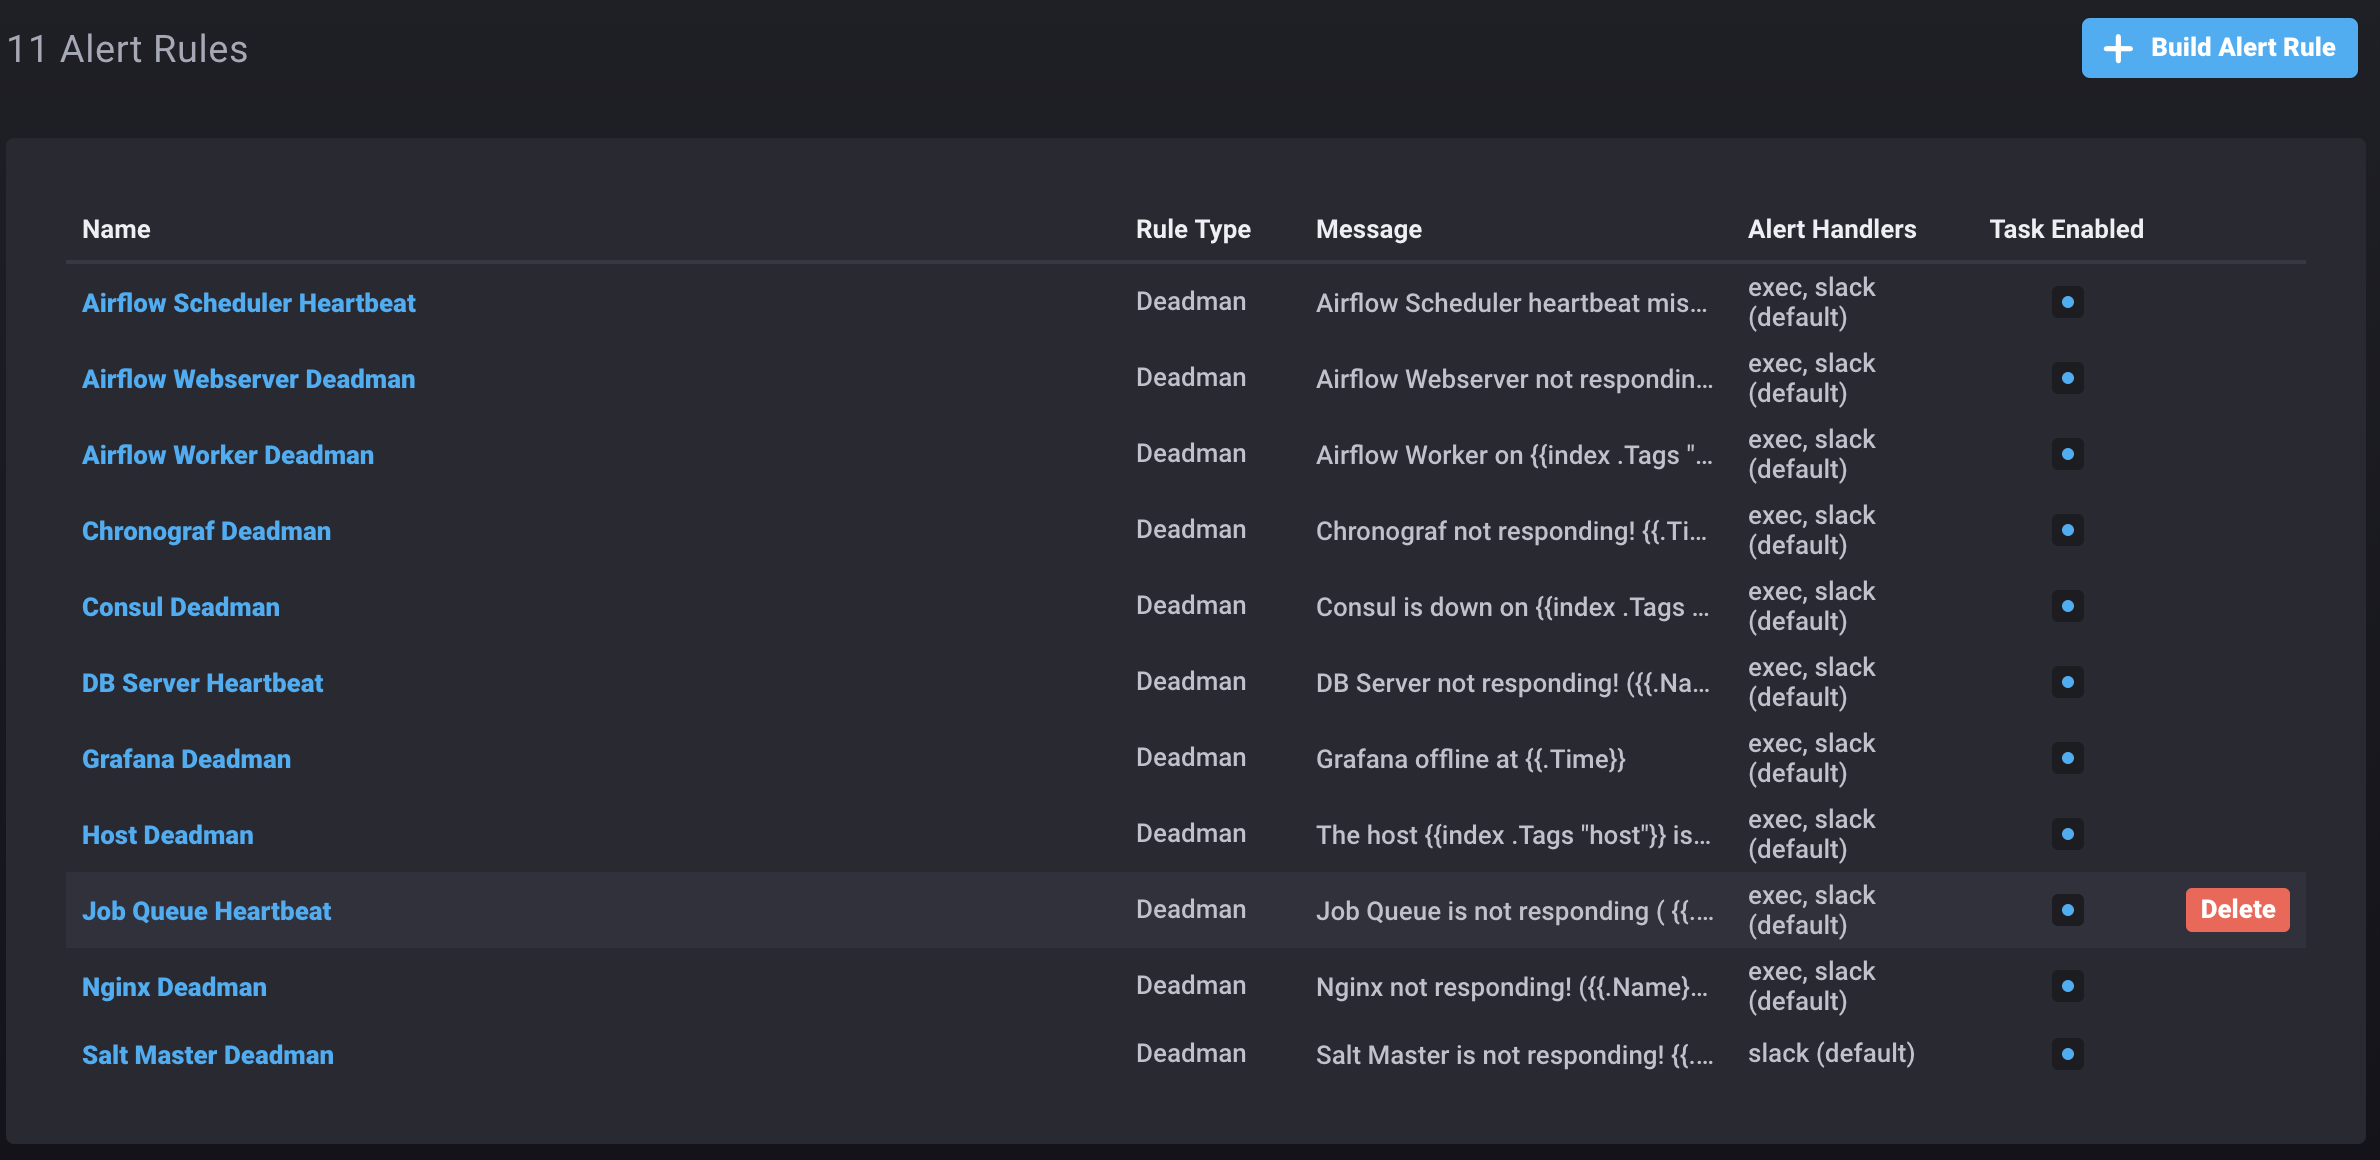
\includegraphics[scale=0.35]{butler_chronograf_tick_list}
    \centering
    \caption {List of rule definitions within chronograf.}
    \label{fig:butler_chronograf_tick_list}
\end{figure} 

Butler defines a variety of rules using TICKscript that capture anomalies that are actionable out of the box, such as those that detect when a variety of services go offline, including - PostgreSQL service, Airflow Scheduler, Airflow Webserver, Airflow Worker, RabbitMQ, Nginx, Grafana, as well as when an entire worker VM goes offline. Each rule needs to be registered with kapacitor and Butler uses the standard Saltstack configuration mechanism to register these rules within the \mintinline{shell}{deploy_ticks} Salt state. There exists an open source Graphical User Interface called chronograf\autocite{chronograf} that allows for visualization and manual inspection and editing of kapacitor rules and the underlying InfluxDB metrics, and Butler makes use of this GUI, see Figures \ref{fig:butler_chronograf_tick_list}, \ref{fig:butler_chronograf_alert_history}.

\begin{figure}[h]
    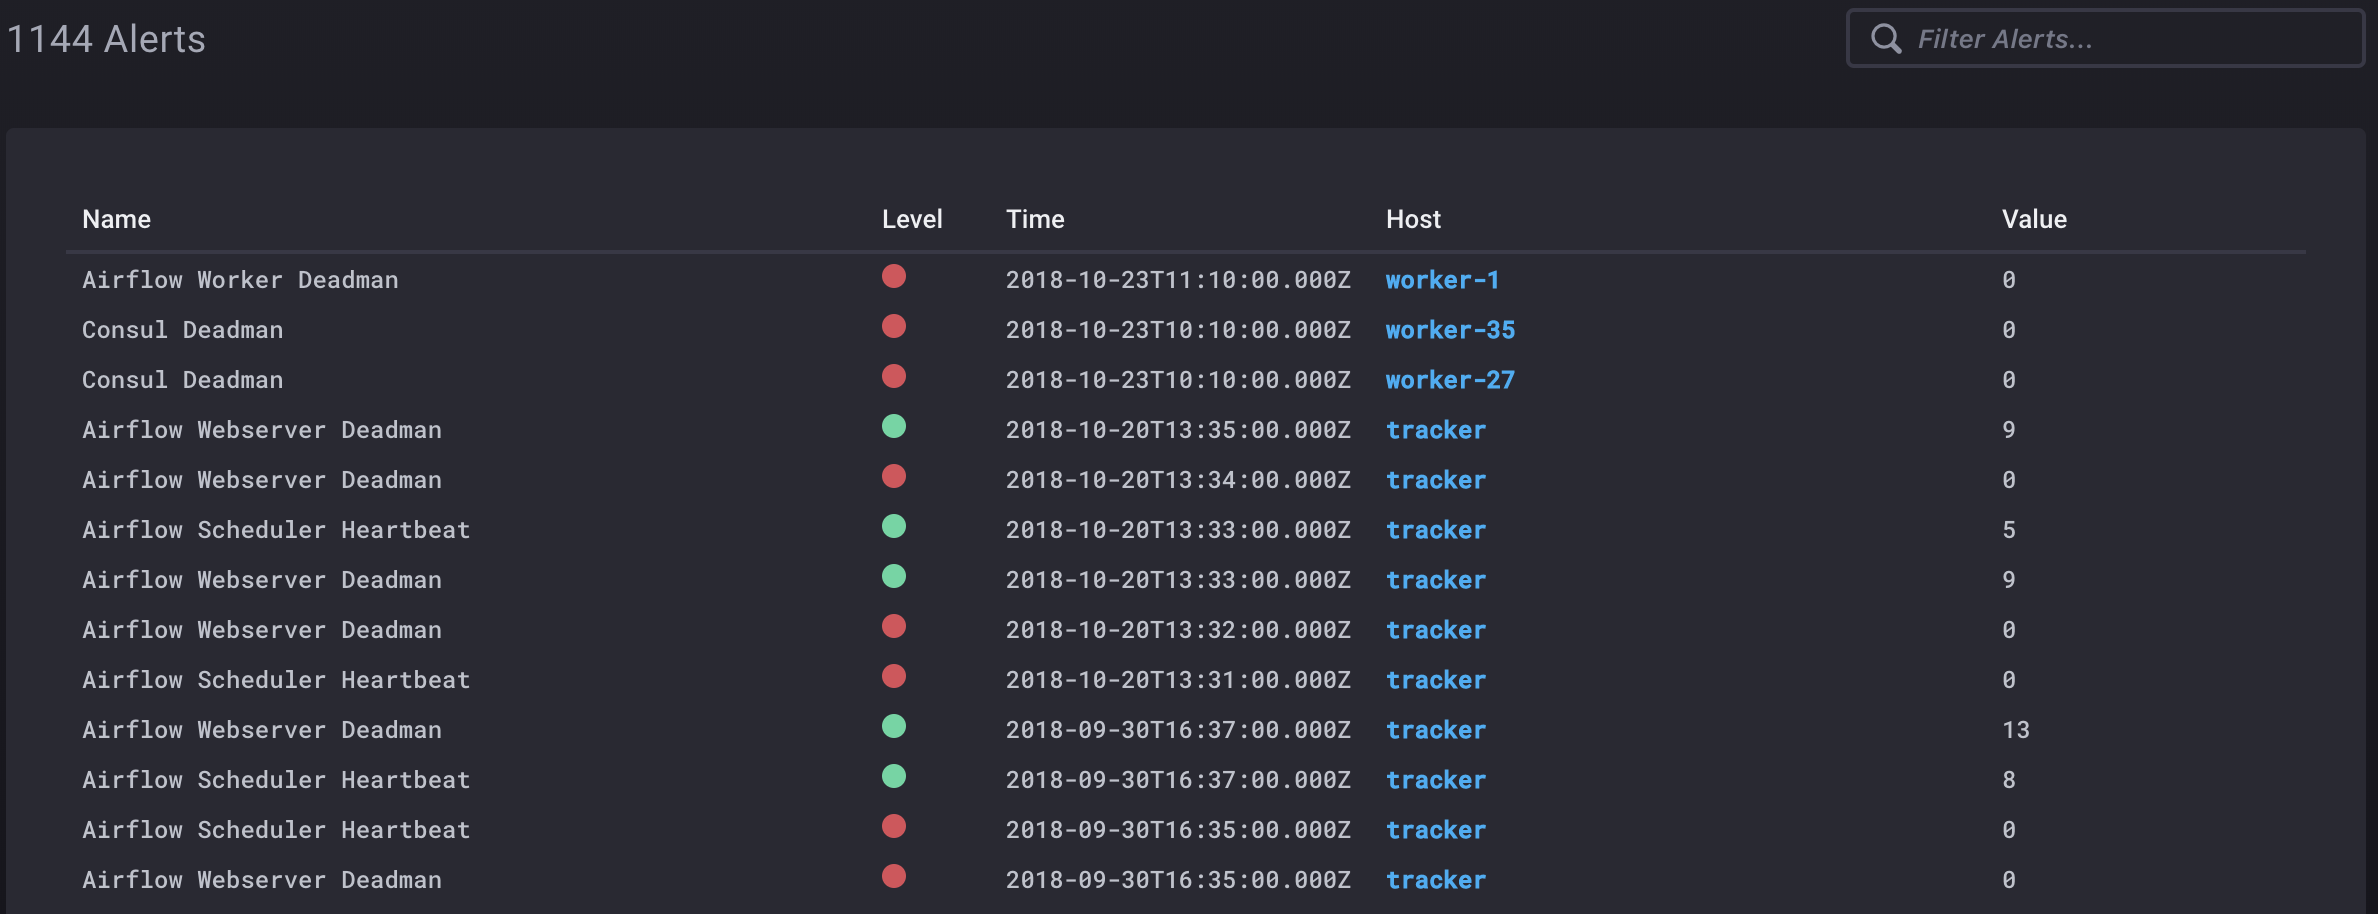
\includegraphics[scale=0.35]{butler_chronograf_alert_history}
    \centering
    \caption {Butler alert history.}
    \label{fig:butler_chronograf_alert_history}
\end{figure} 

\subsubsection{Executing Self-Healing}

Metrics are comprehensively collected within Butler and anomaly detection signals are generated via a set of rules as previously described, but the actual automated self-healing capabilities require a separate component and no generic open source components exist that accomplish this. We thus implement a custom Self-Healing Agent within Butler. The functionality is exposed as a Python package with a CLI interface that is able to accomplish a number of healing tasks on various machines in the Butler cluster.

The self-healing agent relies on the configuration management capabilities available in Butler via Saltstack in order to communicate healing instructions to other hosts. Specifically, Saltstack provides a programmatic interface through which a salt-master can be controlled. This interface is called salt-api. In addition, there exists a module called \mintinline{shell}{pepper} that allows for the salt-api to be communicated with by a remote program via openssl. Butler uses this mechanism to communicate with, and restart various failed services in an automated fashion. For instance, in the case of a failed Airflow Scheduler service (see Listing \ref{lst:self_healing_airflow_scheduler_restart}), the local telegraf metrics collector monitors the \mintinline{shell}{airflow-scheduler} service, and sends updated metrics to the monitoring-server every 10 seconds, where the data is stored in InfluxDB. A kapacitor rule runs on the monitoring-server every 10 seconds and evaluates whether the \mintinline{shell}{airflow-scheduler} is still sending data. If there is no data for longer than 3 minutes, the rule is triggered. As a result the Self-Healing Agent is requested to restart the \mintinline{shell}{airflow-scheduler} service. The agent itself does not know how to communicate with other machines in the cluster, but knows how to communicate with the salt-master. It establishes a salt-api connection to the salt-master and asks for the VM that has the tracker role to restart its \mintinline{shell}{airflow-scheduler} service. The salt-master knows about all of the VMs in the Butler cluster and issues the restart service command, placing the service back in a functioning state. A Slack notification is sent to alert a human operator that an outage has occurred and has been resolved. The total time of the outage is slightly longer than 3 minutes.

\begin{figure}[h]
    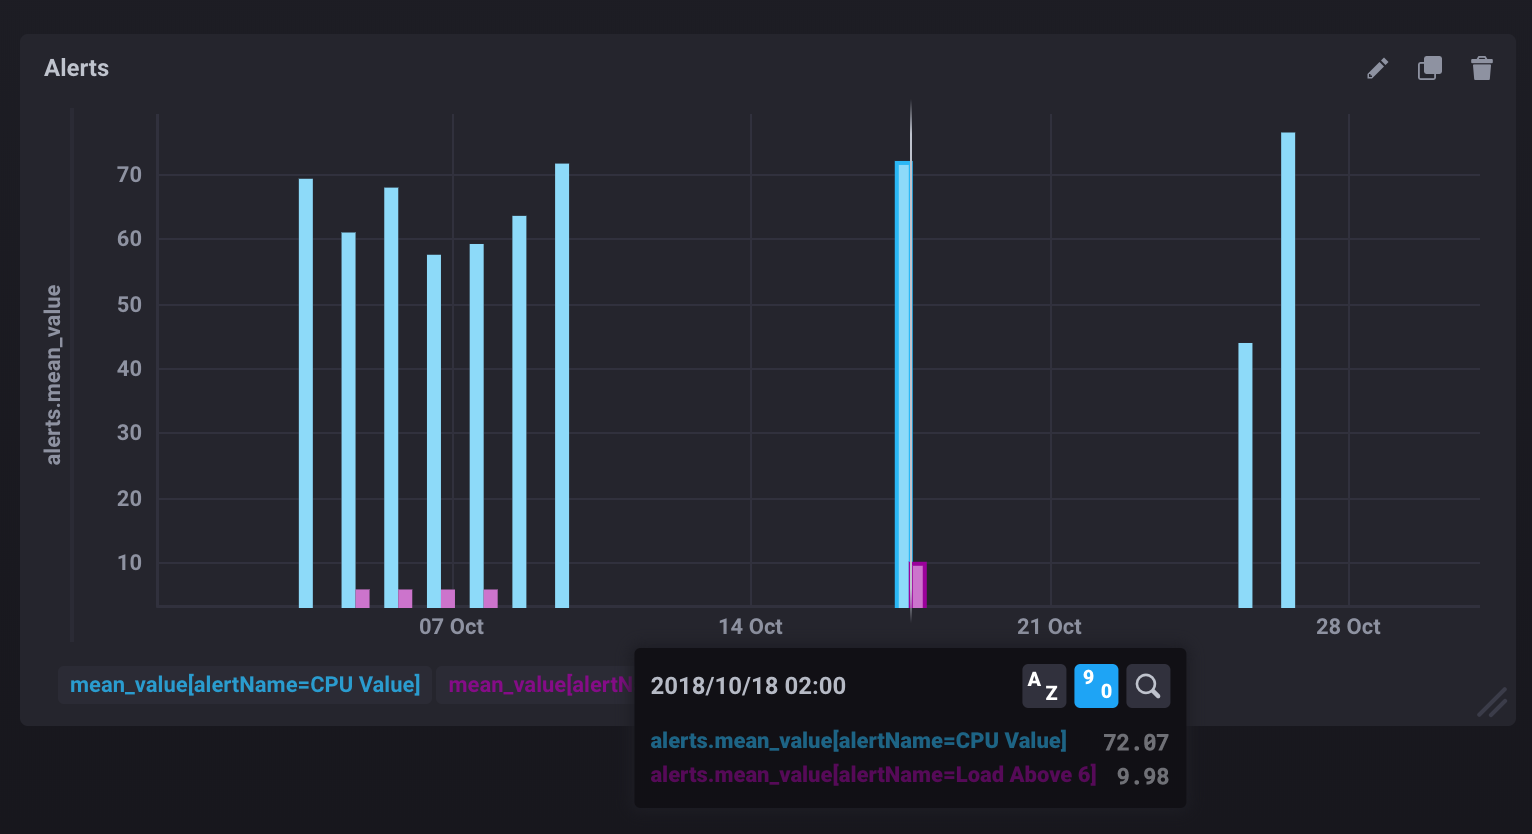
\includegraphics[scale=0.5]{butler_chronograf_alert_barchart}
    \centering
    \caption {Butler timeline of alerts for high CPU utilization.}
    \label{fig:butler_chronograf_alert_barchart}
\end{figure} 




\subsection{Service Discovery} 
\label{sec:design_consul}

The Butler framework consists of many different services that reside on a number of different servers and need to be able to communicate with each other. To accomplish this in a flexible manner we need to establish a Service Registry so that IP addresses of servers that host particular services can be looked up by service name. To accomplish this Butler uses an Open Source service discovery framework called Consul\autocite{Consul_by_HashiCorp}.

Consul provides a cross-data-center distributed Service Name Registry that is available via HTTP and DNS protocols. In addition to registry capabilities Consul provides basic health checks for the underlying services, testing whether the IP and port the service is supposed to be listening on are actually reachable.

\begin{figure}[h]
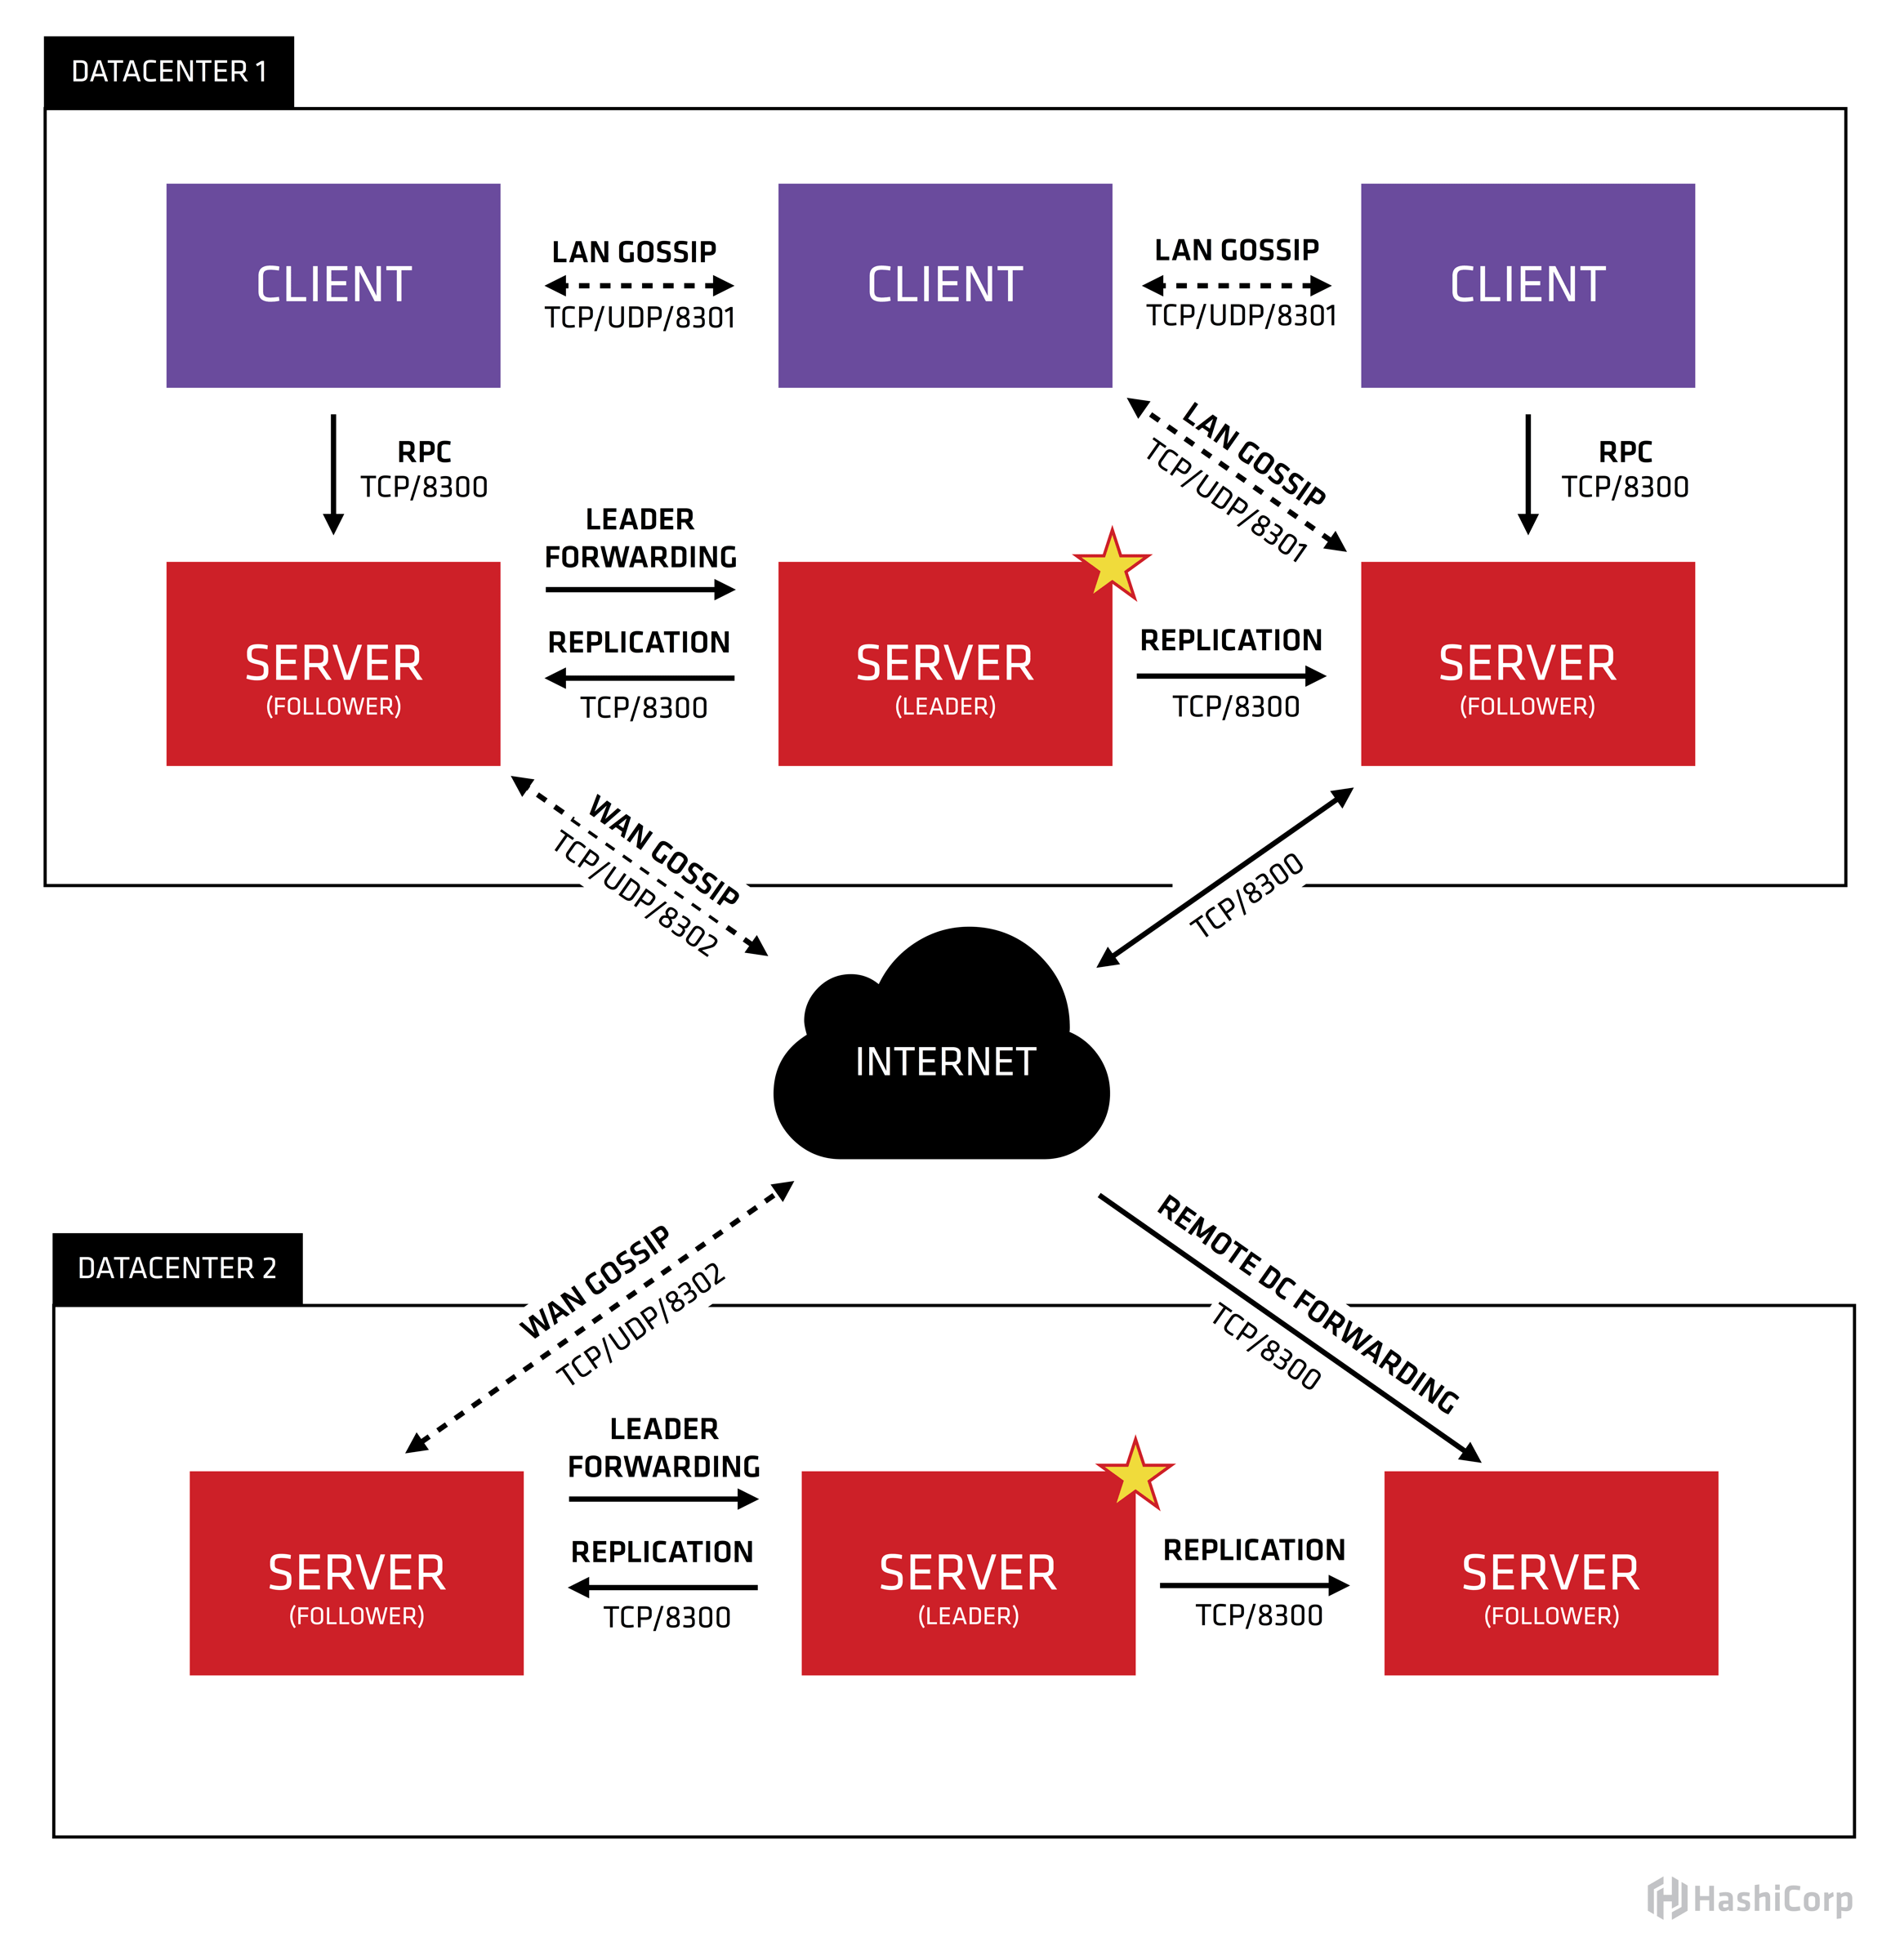
\includegraphics[scale=0.1]{consul_architecture}
\centering
\caption {Consul high level architecture (from \url{https://www.consul.io/docs/internals/architecture.html)}.}
\label{fig:consul_architecture}
\end{figure} 

Each VM in the cluster runs a Consul Agent which can be run in Server and Client modes. The set of Consul Servers form a Raft cluster and provide consensus-based responses to service lookup requests from clients. When new VMs are started they need to join the Consul cluster in order to be able to perform lookups, doing so requires knowing the IP address of at least one server. In Butler we use Saltstack's configuration capabilities to convey a Consul Server's IP address to any new VM that is brought up. 

Registering a service with Consul is a matter of creating a JSON formatted configuration file that declares the service (see Listing \ref{lst:consul_postgres_service}). A Consul agent running on that VM will ingest the service definition and relay it to a Consul Server which will then circulate it amongst the other servers. The service will then be available for DNS lookups. The service from Listing \ref{lst:consul_postgres_service} will have the name \mintinline{shell}{postgresql.service.consul}, for example.



	

\chapter{The Butler Framework - Implementation and Experimental Validation} \label{ch:butler_implementation}
%The Butler framework has been built to enable large-scale scientific analyses in the cloud and the largest set of analyses that have been performed using this framework to date have been the Germline analyses for the Pan-Cancer Analysis of Whole Genomes Project on the EBI Embassy Cloud. We describe the nature of these analyses as well as the details of the Butler deployment on the Embassy Cloud next.

\section{Deployment on EMBL/EBI Embassy Cloud}

The EMBL/EBI Embassy Cloud\autocite{cook2016european} is an academic cloud computing center which runs an Openstack-based environment. The Embassy Cloud plays a key role in the PCAWG project by donating substantial storage and cloud computing capacity over the course of 3 years. The total amount of resources dedicated to the project by the Embassy Cloud is:

\begin{itemize}
\item 1 PB Isilon storage shared over NFS
\item 1500 compute cores
\item 6 TB RAM
\item 40 TB local SSD storage
\item 10 Gb network
\end{itemize}

These resources have been used to host one of the seven PCAWG GNOS repositories that exist worldwide, as well as performing a number of scientific analyses for the project. We have used Butler extensively on the Embassy Cloud in order to carry out the germline analyses for PCAWG-8 Working Group.

\begin{figure}[H]
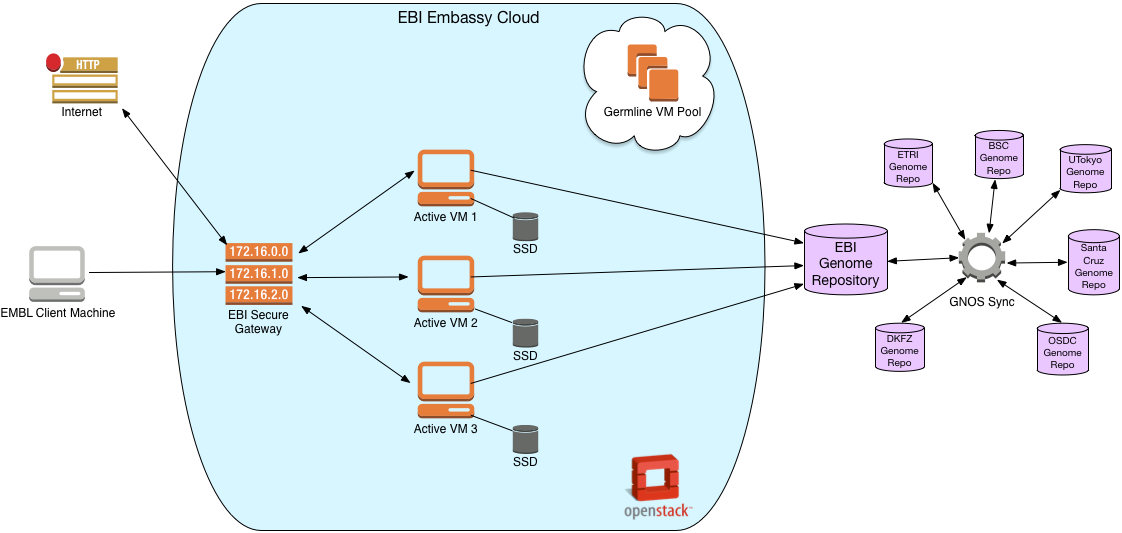
\includegraphics[width=\textwidth]{embassy_architecture}
\centering
\caption {Embassy Cloud Architecture}
\label{fig:embassy_architecture}
\end{figure}

\subsubsection{Embassy Cloud Architecture}

Figure \ref{fig:embassy_architecture} shows the general high-level architecture of the Germline Working Group's tenant within the EMBL/EBI's Embassy Cloud. Because of the sensitive nature of the genetic data that is stored at Embassy there are several security mechanisms in place. The Virtual Machines are hidden behind a secure gateway and are not visible to the external network. The secure gateway maintains a hand-curated list of IP addresses that are allowed to connect to it from the Internet. Currently this list contains several IP addresses of research institutions that are part of the PCAWG project. Beyond the gateway is a bastion host - a Virtual Machine which serves as the entry-point into the cloud environment. Individual users can establish SSH sessions to the bastion host using their SSH key. From the bastion host the user can establish key-based SSH access to other Virtual Machines within the tenancy. 

Authenticated Web-based access to the Openstack dashboard (Figure \ref{fig:embassy_dashboard}) provides a conventional method for the users to create and manage Virtual Machines.

\begin{figure}[H]
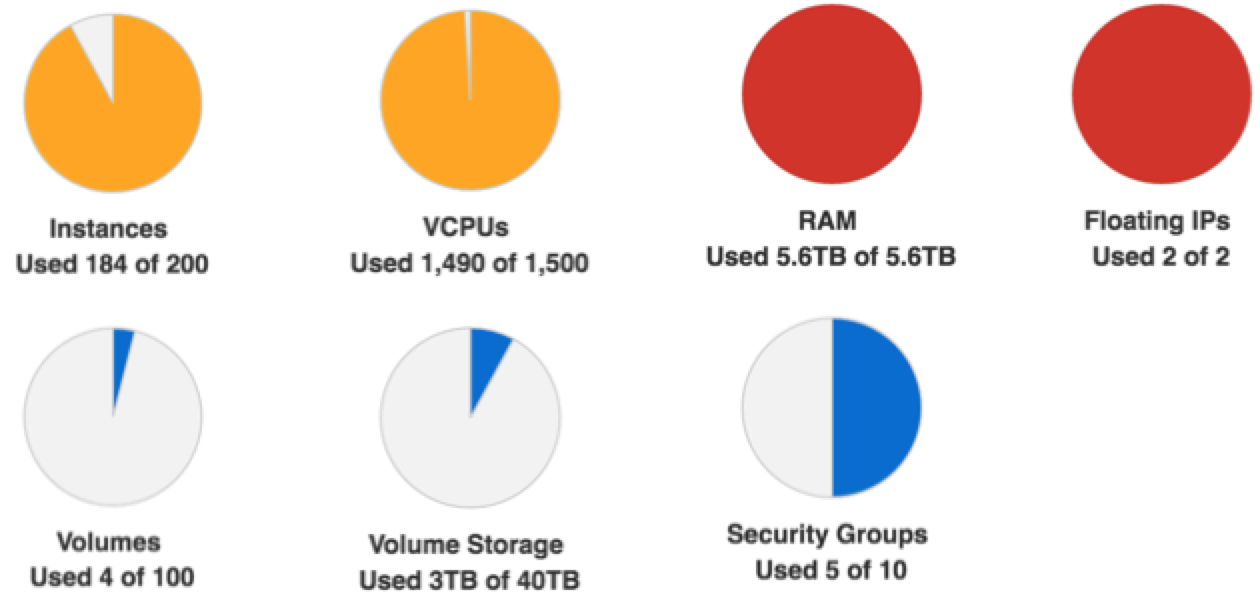
\includegraphics[width=\textwidth]{embassy_dashboard}
\centering
\caption {Embassy Cloud Dashboard}
\label{fig:embassy_dashboard}
\end{figure}

\subsubsection{Access to PCAWG Data}
\label{sec:pcawg_data_access}

The raw data for PCAWG is hosted in a distributed manner in GNOS repositories. A data synchronization mechanism copies data between repositories when necessary. The EMBL/EBI GNOS repository is one of the most complete sources of PCAWG data, hosting close to 1PB of data for the project. Although typically access to the GNOS repository is only available via a GNOS client the Embassy Cloud IT team has made a special provision for the Germline Working Group to allow access to the underlying data via an NFS share. This allows Butler-based workflows to have more efficient access to the data.

The PCAWG project periodically publishes an official list of all samples that are part of the project. In order to facilitate accurate sample tracking for analysis purposes we have built a Sample Tracking Database on top of PostgreSQL and SQLAlchemy. There are two tables \mintinline{sql}{pcawg_samples} and \mintinline{sql}{sample_locations}. \mintinline{sql}{pcawg_samples} maintains a list of official samples along with their accompanying metadata while \mintinline{sql}{sample_locations} contains a set of file paths that indicate where to find each sample on the Embassy Cloud file server. This table is populated by a script that crawls the directory structure looking for samples that are part of the official list.

\subsubsection{Butler deployment}

Butler has been deployed on the Embassy Cloud since March, 2016 and has been used extensively to carry out analyses for the Germline Working Group.

To deploy Butler on the 1500 core cluster we set up five different profiles of VMs, each playing a number of different roles (Table \ref{tab:embassy_deployment}):

\begin{table}[H] 
\renewcommand{\arraystretch}{2} 
\centering
\begin{tabu} to \linewidth {X[3]X[1,r]X[2,r]X[4]X[4]X[1,r]}
\toprule
Machine & CPU & RAM (GB) & Disk (GB) & Roles & Count\\
\midrule
salt-master & 4 & 6 & 50 ephemeral\newline 1000 block for metrics storage & salt-master \newline consul-bootstrap\newline monitoring-server & 1\\
tracker & 4 & 4 & 40 ephemeral \newline 1000 block for elasticsearch & tracker \newline consul-server \newline elasticsearch & 1\\
job-queue & 4 & 4 & 40 ephemeral & job-queue \newline consul-client & 1\\
db-server & 8 & 16 & 80 ephemeral \newline1000 block for db & db-server \newline consul-client & 1\\
worker & 8 & 32 & 100 ephemeral & worker \newline germline \newline consul-client & 175\\
\bottomrule
\end{tabu}
\caption{Butler deployment on Embassy Cloud}
\label{tab:embassy_deployment}
\end{table} 

Each profile is defined separately via Terraform and uses Saltstack roles for configuration. The user can check out the Butler github repository to their local machine and once they install Terraform locally, and provided that they are able to connect to the EBI Secure Gateway (Figure \ref{fig:embassy_architecture}) they can fully commandeer the provisioning process from the local machine via Terraform.

Figure \ref{fig:embassy_butler_deployment_architecture} provides a diagrammatic view of the deployment of various Butler components on the Embassy Cloud.

\begin{figure}[H]
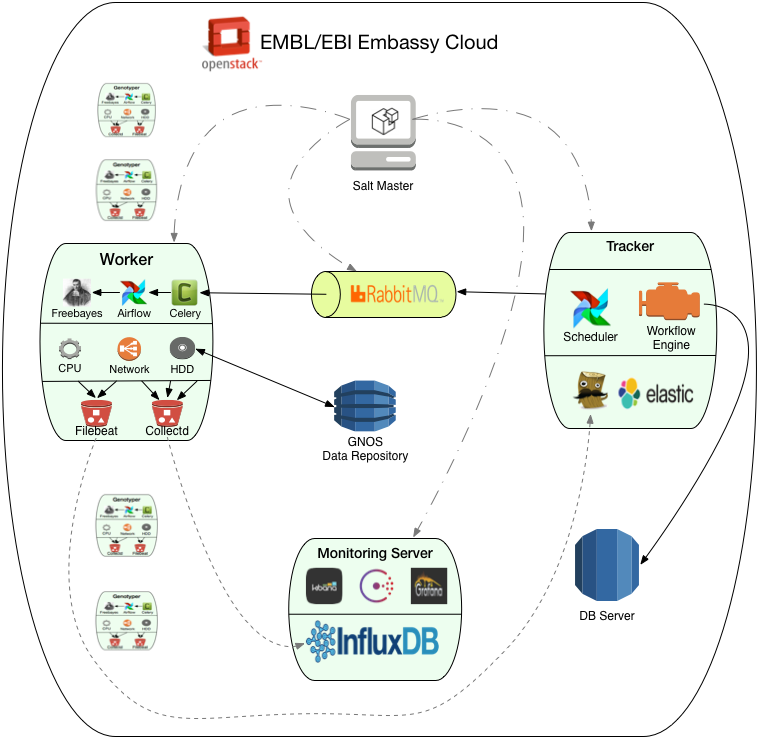
\includegraphics[width=\textwidth]{embassy_butler_deployment_architecture}
\centering
\caption {Butler Deployment Architecture}
\label{fig:embassy_butler_deployment_architecture}
\end{figure}

The cluster is bootstrapped via the salt-master VM. This VM is started first whenever the cluster needs to be recreated from scratch. The salt-master is started with a minimal OS image for speed and all of the other configurations are delivered via Saltstack itself. The IP of the salt-master machine is retained so that it can be passed on to the other VMs upon creation so that they know how to connect to the master when they boot up. The salt-master VM plays two other roles (Table \ref{tab:embassy_deployment}) in this deployment in order to maximize resource utilization (since Saltstack is a light resource consumer) - consul-bootstrap, and monitoring-server. The consul-bootstrap role conveys the responsibility for starting up the Consul Service Discovery mechanism to the salt-master. When set up in bootstrap mode, consul waits for one more consul server to join the cluster, before quorum is reached and the cluster becomes fully operational. The monitoring-server role is responsible for installing and configuring InfluxDB and other monitoring components  as well as registering them with Consul so that metrics can start being recorded. We also attach a 1TB block storage volume for the metrics database so that it can survive cluster crashes and tear-downs. If the monitoring server needs to be recreated, the block storage volume simply needs to be reattached to the new Monitoring Server VM.

The tracker VM is responsible for running various Airflow components such as the - Scheduler, Webserver, and Flower (Section \ref{sec:design_workflow_system}). Additionally we deploy the Butler tracker module (Section \ref{sec:analysis_tracker})to this VM, thus the tracker VM acts as the main control point of the system from which analyses are launched and monitored. This VM additionally has the elasticsearch role which designates it as the location of the Logstash and Elasticsearch components (Section \ref{sec:design_log_collection}). To persist the search index we attach an additional 1TB block storage volume. The consul-server role allows the cluster, once the tracker VM is brought up, to reach quorum necessary for full Consul functionality. 

The job-queue VM is responsible for hosting the RabbitMQ server which holds all of the in-flight workflow tasks. Because the resources of the job-queue are heavily taxed by communication with all of the worker VMs in the cluster we do not assign any additional roles to this host.

The db-server is responsible for hosting most of the databases used by Butler. This VM runs an instance of PostgreSQL Server and hosts the Run Tracking DB, Airflow DB, and Sample Tracking DB. The 1TB block storage volume serves as the backing storage mechanism. 

The worker VMs are the workhorses of the Butler cluster. In its current deployment (October 2016) there are 175 8-core worker machines that are dedicated to running Butler workflows. The worker role ensures that Airflow client modules are installed and loaded on each worker. The germline role additionally loads the workflows and analyses that are relevant to the PCAWG Germline Working Group. 


\section{PCAWG Germline Analyses}

The PCAWG project is divided into a set of working groups. Each group has a different set of research interests and technical activities that it is contributing to the overall project effort.  The goal of the Germline Working Group, also known as PCAWG-8, is to study the distribution of germline (mutations that are inherited from one's parents) polymorphisms within the PCAWG cohort of 2834 cancer patients and gain a better understanding of how these germline polymorphisms affect various aspects of the patients' disease, for instance whether they affect disease progression, likelihood of survival, or any number of molecular-level traits such as DNA repair, propensity towards certain types of mutations, or gene dysregulation.

To enable these analyses the goal of the Germline Working Group is to produce a full set of high quality genotyped germline variants. Doing so requires carrying out a significant number of computational steps that use the entire 725 TB raw data set. These steps are as follows:

\begin{description}
\item [Variant Discovery] - Use a set of algorithms that look at each location in the genome and try to determine where the genome differs from the known reference sequence.
\item [Variant Genotyping] - Using a set of variant sites produced by Variant Discovery and determine an accurate genotype at the variant position for all donors in the cohort.
\item [Variant Filtration] - Filter out false positive calls introduced by the previous steps.
\item [Genotype Phasing] - Use an algorithm to determine which chromosome (of the pair) each variant belongs to.
\item [Data Submission] - Prepare metadata and submit the resulting call-set to a centralized data repository.
\end{description}

\subsection{Variant Discovery}
\label{sec:variant_discovery}

There exist multiple algorithms for variant discovery and each algorithm has a unique set of features. As a result, they typically produce call-sets that only overlap on a subset of the values\autocite{li2014towards}. In order to improve the sensitivity of the call-set the Germline Working Group is producing three independent discovery call sets via three different algorithms - Freebayes\autocite{garrison2012haplotype}, GATK HaplotypeCaller\autocite{depristo2011framework}, and RTG\autocite{cleary2014joint}. These call-sets are then merged via a two-out-of-three criterion i.e. a variant is retained if it is called by at least 2 of the three pipelines. This approach produces a more sensitive call-set than via any of the tools individually.

The GATK HaplotypeCaller data set has been produced by the Broad Institute, the RTG set has been produced by Stanford University, and the Freebayes data set has been produced using a Butler workflow on the EBI Embassy Cloud.

\subsubsection{The freebayes Butler workflow}
The freebayes workflow parallelizes its work by splitting each sample by chromosome to reduce the amount of time it takes to process a single sample. Although the chromosomes have vastly different sizes (see Table \ref{tab:chromosome_sizes}), and thus individual jobs have different runtimes, when many samples are processed, there is little practical impact on when the entire batch of samples is completed.

\begin{table}[H]
\label{tab:chromosome_sizes}
\renewcommand{\arraystretch}{1.2} 
\centering
\begin{tabular}{@{}lll@{}}
\toprule
Chromosome & Size(base pairs)\\
\midrule
1 & 249,250,621\\
2 & 243,199,373\\
3 & 198,022,430\\
4 & 191,154,276\\
5 & 180,915,260\\
6 & 171,115,067\\
7 & 159,138,663\\
8 & 146,364,022\\
9 & 141,213,431\\
10 & 135,534,747\\
11 & 135,006,516\\
12 & 133,851,895\\
13 & 115,169,878\\
14 & 107,349,540\\
15 & 102,531,392\\
16 & 90,354,753\\
17 & 81,195,210\\
18 & 78,077,248\\
19 & 59,128,983\\
20 & 63,025,520\\
21 & 48,129,895\\
22 & 51,304,566\\
X & 155,270,560\\
Y & 59,373,566\\
\bottomrule
\end{tabular}
\caption{Human chromosome size distribution}
\end{table}

Overall, most Butler workflows that carry out an analysis follow a similar structure - an Analysis Run is started, access to the sample is validated, the analysis steps are carried out (possibly with branching), and the Analysis Run is completed (see Figure \ref{fig:butler_freebayes_workflow}).

\begin{figure}[H]
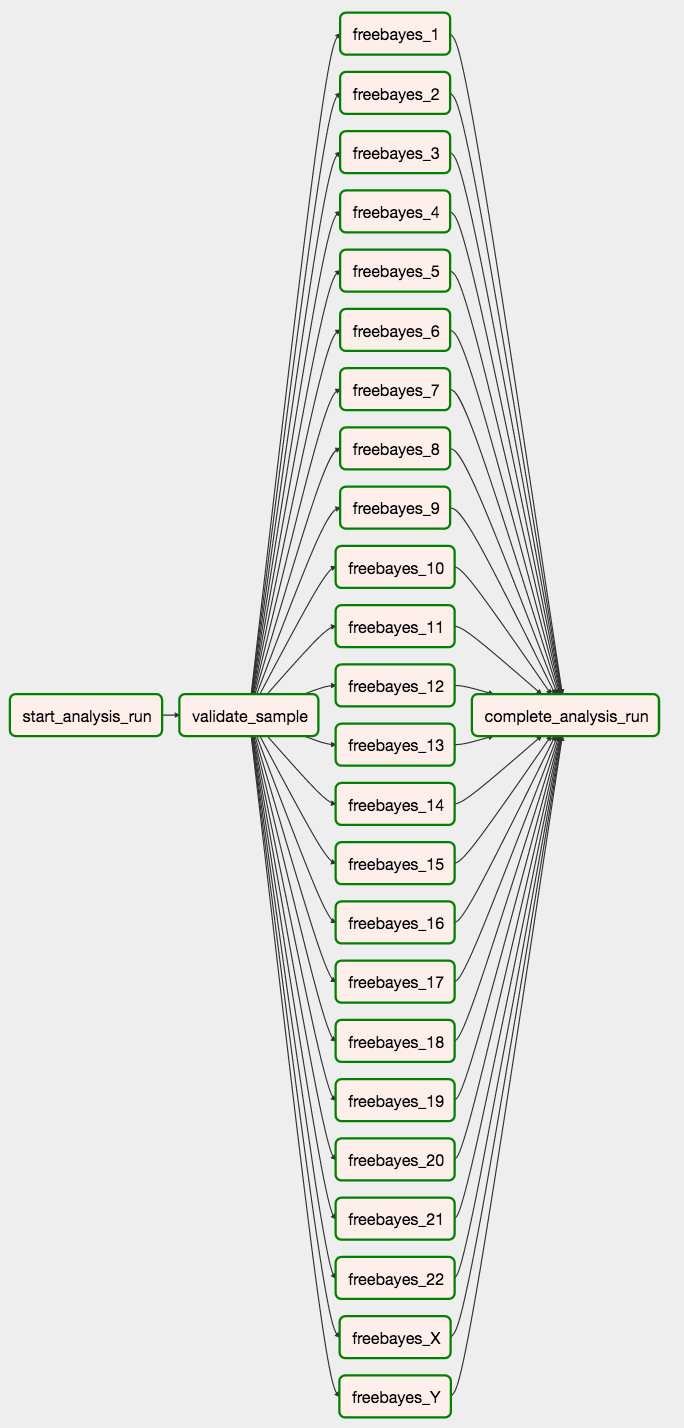
\includegraphics[scale=0.7]{butler_freebayes_workflow}
\centering
\caption {Structure of the Butler freebayes workflow}
\label{fig:butler_freebayes_workflow}
\end{figure}

Because of the largely common structure between workflows a large degree of code reuse is possible, thus most of the methods reside in the workflow\_common submodule of the tracker module (see Section \ref{sec:analysis_tracker}) and are invoked for each workflow.

A full listing of the source code for the freebayes workflow is provided in Listing \ref{lst:freebayes_workflow} and is discussed next. 




Lines 81-127 of the source code define the workflow structure, first by declaring an instance of type \mintinline{python}{DAG}, and then by defining a sequence of workflow tasks. In this case each task is a Python callable. The loop on line 117 defines one workflow task for each chromosome in the predefined list. The order of task execution is defined by calling a task's \mintinline{python}{set_upstream()} method, such as on lines 109 and 127 of the listing. Default parallelism behaviour is specified on line 92 where the maximum number of active workflow runs is defined to be 2000, and the maximum number of active workflow tasks is defined to be 10,000. If more workflows than the maximum get scheduled, they will be queued until some workflow instances complete.

The bulk of the body of the workflow definition (lines 14-78) is dedicated to the implementation of a single function - \mintinline{python}{run_freebayes(**kwargs)} which manages the invocation of the freebayes tool on a single chromosome of a sample. Line 16 gets the effective configuration dictionary (see Section \ref{sec:workflow_configuration_design}) which contains the merged configuration parameters from Workflow (Listing \ref{lst:freebayes_workflow_config}), Analysis (Listing \ref{lst:freebayes_discovery_config}), and Analysis Run (Listing \ref{lst:freebayes_discovery_run_config}) levels. 


\captionof{listing}{Workflow-level configuration for freebayes workflow.\label{lst:freebayes_workflow_config}}
\begin{minted}
[
breaklines=true,
linenos,
fontsize=\footnotesize,
frame=lines,
framesep=2mm,
baselinestretch=1.2
]
{json}
{
	"contig_names": ["1", "2", "3", "4", "5", "6", "7", "8", "9", "10",
                "11", "12", "13", "14", "15", "16", "17", "18", "19", 
                "20", "21", "22", "X", "Y"],
	"reference_location": "/reference/genome.fa",
	"bgzip": {
		"path": "/usr/local/bin/bgzip",
		"flags": ""
	},
	"tabix": {
		"path": "/usr/local/bin/tabix",
		"flags": "-f -p vcf"
	},
	"rsync": {
		"flags": "-a -v --remove-source-files"
	},
	"freebayes": {
		"path": "/bin/freebayes"
	}
}
\end{minted}

The workflow-level configurations contain values that should generally be applicable to any invocation of the workflow. In exceptional cases these can be overridden at Analysis and 
Analysis Run levels. For the freebayes workflow these settings include a list of chromosomes to call, the path to the human reference genome, and paths to various tools used within the workflow

\captionof{listing}{Analysis-level configuration for freebayes variant discovery analysis.\label{lst:freebayes_discovery_config}}
\begin{minted}
[
breaklines=true,
linenos,
fontsize=\footnotesize,
frame=lines,
framesep=2mm,
baselinestretch=1.2
]
{json}
{
	"results_base_path": "/shared/data/results/discovery/",
	"results_local_path": "/tmp/discovery/",
	"freebayes": {
		"mode": "discovery",
		"flags": "--min-repeat-entropy 1 --report-genotype-likelihood-max"
	}
}
\end{minted}

Since our analysis focuses on variant discovery, the Analysis-level JSON configuration file contains freebayes flags to set up discovery mode, as well as setting up a location for where to store the analysis results and which directory to use as local scratch space.
 
\captionof{listing}{AnalysisRun-level configuration for a single sample in freebayes variant discovery analysis. \label{lst:freebayes_discovery_run_config}}
\begin{minted}
[
breaklines=true,
linenos,
fontsize=\footnotesize,
frame=lines,
framesep=2mm,
baselinestretch=1.2
]
{json}
{
	"sample": {
		"sample_location": "/gnosdata/tcga/PCAWG.67455c36-aa47-4cc4-8b6d-9a9012b616ed.bam",
		"donor_index": 0,
		"sample_id": "f22a72c5-73c8-478d-b03e-04599b9d5321"
	}
}
\end{minted}

Listing \ref{lst:freebayes_discovery_run_config} provides an example of what an AnaysisRun-level configuration looks like. This configuration is concerned with supplying sample level configuration values, such as the sample\_id and sample\_location.

After all of the necessary parameters are extracted from the configuration and command invocation is set up lines 71-75 of Listing \ref{lst:freebayes_workflow} actually invoke a series of commands that perform the bulk of the analysis - calling \mintinline{shell}{freebayes} to generate the discovery call-set, followed by converting the call-set into a binary compressed format (with \mintinline{shell}{bgzip}), followed by generating an index file for record-based random access into the binary file (with \mintinline{shell}{tabix}), and followed by an \mintinline{shell}{rsync} to the shared results storage indicated in the configuration.

The workflow is distributed to all worker nodes in the cluster via a Saltstack state as shown in Listing \ref{lst:workflow_deployment}.



\subsubsection{AnalysisRun configurations for freebayes workflow}

While each workflow only has one workflow-level configuration and possibly a few dozen analysis-level configurations, there needs to be one analysis run-level configuration generated for each sample under analysis, thus resulting in thousands of these configurations being generated for each analysis. The most effective method for accomplishing this is via a script. We utilize two databases - the Run Tracking Database (Section \ref{sec:analysis_tracker}), and the Sample Tracking Database (Section \ref{sec:pcawg_data_access}) in order to generate a list of samples for which there are no Analysis Runs present for a given Analysis yet. To generate our result-set we utilize the SQLAlchemy Object-Relational Mapping framework (see \ref{sec:available_samples}).

\captionof{listing}{SQLAlchemy query to generate available samples.\label{lst:available_samples}}
\begin{minted}
[
breaklines=true,
fontsize=\footnotesize,
linenos,
frame=lines,
framesep=2mm,
baselinestretch=1.2
]
{python}
current_runs = run_session.query(Configuration.config[("sample"," sample_id")].astext).\
        join(AnalysisRun, AnalysisRun.config_id == Configuration.config_id).\
        join(Analysis, Analysis.analysis_id == AnalysisRun.analysis_id).\
        filter(and_(Analysis.analysis_id == analysis_id, AnalysisRun.run_status != tracker.model.analysis_run.RUN_STATUS_ERROR)).all()
        
available_samples = sample_session.query(PCAWGSample.index.label("index"), sample_id.label("sample_id"), sample_location.label("sample_location")).\
        join(SampleLocation, PCAWGSample.index == SampleLocation.donor_index).\
        filter(and_(sample_location != None, sample_id.notin_(current_runs))).\
        limit(num_runs).all()
\end{minted}

The final script is wrapped in a Command Line Interface to improve the user experience. It supports the following parameters:

\begin{description}
\item [analysis\_id] - The id of the Analysis for which to generate Analysis Run configs.
\item [num\_runs] - The number of runs to generate. The actual number of runs will be \mintinline{shell }{min(num_runs, available_runs)}
\item [tissue\_type] - Whether to generate the Analysis Runs for tumor or normal tissue samples.
\item [config\_location] - File path where to store the resulting Analysis Run configs.
\end{description}

Thus, a full invocation would look like:

\begin{minted}
[breaklines=true]
{shell}
python prepare_freebayes_genotyping_config.py create-configs -a 3 -n 150 -t normal -c /config_file_location/
\end{minted}

This would generate at most 150 JSON files with configurations for Analysis ID 3 and normal tissue samples, storing them in /config\_file\_location/ which could be used to start workflow instances for this analysis.


\subsection{Variant Genotyping}

Genotyping refers to accurately determining for each sample and at each variant position what are the two nucleotide bases (one for each sister chromosome) at that position\autocite{wang1998large}. This analysis involves looking at the DNA reads that overlap each position and evaluating a model for the likelihood of each possible genotype given the data observed in the reads. The genotype with the highest likelihood given the data is selected\autocite{nielsen2011genotype}. To accomplish this task we use a Butler workflow that utilizes freebayes as the computational algorithm underneath the covers. Because the freebayes workflow from Section \ref{sec:variant_discovery} has been built in a generic fashion the only changes that are necessary between discovery and genotyping analyses lie within the analysis configuration.

We see in Listing \ref{lst:genotyping_analysis} that we need to provide a list of variant locations that need to be genotyped, split by chromosome, and stored in VCF format\autocite{danecek2011variant}. Additionally, we provide a set of flags to freebayes that indicate that the tool should be used in genotyping mode.

\subsection{Variant Filtration}

Although utilizing multiple variant callers for variant discovery improves the overall sensitivity it also increases the number of false positives in the call-set. In order to remove the false positive calls the Germline Working Group has undertaken a number of filtration steps. Some of these steps involve machine learning methods that are carried out outside the scope of Butler, but some are based on a set of well-known filtering criteria. These are implemented as a separate Butler workflow.

\begin{figure}[H]
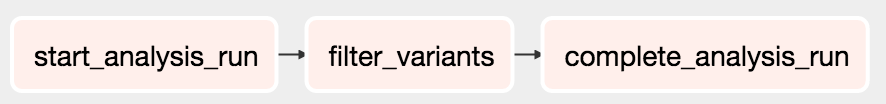
\includegraphics[scale=0.7]{butler_filter_variants_workflow}
\centering
\caption {Structure of the Butler Variant Filtration workflow}
\label{fig:butler_filter_variants_workflow}
\end{figure}

The Filter Variants workflow has a rather simple structure. Bookended by the standard run-start and run-completion tasks is the actual filtration task. This task is implemented as an Airflow PythonOperator and invokes two commands - vcftools\autocite{danecek2011variant} and vt\autocite{tan2015unified}. vcftools is used for actual variant filtering, while vt is used for variant normalization.

\captionof{listing}{Butler Analysis configuration for VCF filtering.\label{lst:filtering_analysis}}
\begin{minted}
[
breaklines=true,
breakanywhere=true,
fontsize=\footnotesize,
linenos,
frame=lines,
framesep=2mm,
baselinestretch=1.2
]
{json}
{
	"results_base_path": "/shared/data/results/discovery_filtered/",
	"results_local_path": "/tmp/discovery_filtered/",
	"vcffilter": {
		"flags": "QUAL > 20 & DP > 3 & QUAL / AO > 2 & SAF > 1 & SAR > 1 & RPR > 1 & RPL > 1"
	},
	"vt": {
		"command": "normalize"
	}
}
\end{minted}

Listing \ref{lst:filtering_analysis} demonstrates the usage of vcftools' flags to achieve variant filtering for PCAWG. 

\subsection {Genotype Phasing}

Because each individual inherits one copy of each chromosome (except for sex chromosomes X and Y) from the mother and one from the father, a variant may lie on one chromosome or the other, or both. It is, thus, important to understand which chromosome each variant lies on in order to inform downstream analyses. This methodology is called statistical phasing and will be carried out by a tool called Shapeit\autocite{delaneau2012linear} outside of Butler.

\subsection {Data Submission}

Once a call-set for each sample is produced and vetted it needs to be submitted to a centralized data repository so that it can be shared with other researchers on the project. There are seven such data repositories throughout the world, each running a software tool called GNOS\autocite{wilks2014cancer} from Annai Systems. A submission to GNOS consists of the call-set data accompanied by an XML-formatted metadata file, that describes the submission. GNOS then uses a proprietary torrent-like protocol for secure file uploads. A Butler workflow implements automated sample submissions to GNOS.

\begin{figure}[H]
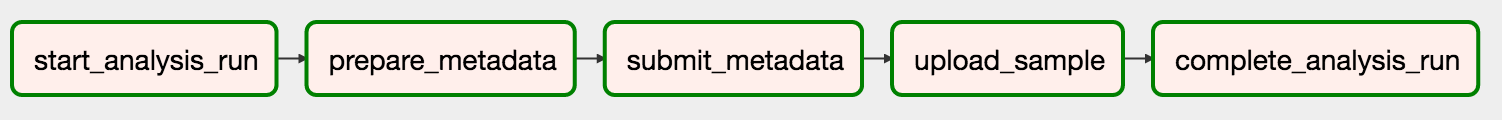
\includegraphics[width=\textwidth]{butler_gtupload_workflow}
\centering
\caption {Structure of the Butler Data Submission workflow}
\label{fig:butler_gtupload_workflow}
\end{figure}

The Data Submission workflow (Figure \ref{fig:butler_gtupload_workflow}) follows a linear sequence of events implemented as Airflow PythonOperators. The data submission is a three step process where the first action is to prepare a sample's accompanying metadata submission, the second is to submit this metadata to a GNOS repository of choice, which generates a manifest in return, and the third step is to upload the actual data to the same repository using the manifest. See Listing \ref{lst:gtupload_workflow}

In order to be able to successfully submit a sample, the sample, along with its accompanying metadata must be placed in a separate directory whose name is a Universally Unique Identifier (UUID) - this UUID will become an identifier for the submission on the GNOS server. Furthermore, the metadata file - an XML document, must be populated with descriptions of the analysis steps taken to produce the sample. We generate this file in Butler's workflow with the aid of an XML template (see Listing \ref{lst:gtupload_analysis} template declaration) and using Python's \mintinline{python}{etree} module.


Once the submission is ready, the actual process of submission is carried out using the \mintinline{shell}{cgsubmit} tool by Annai Systems. It is important which GNOS repository a sample ends up in as not all repositories have permissions to host all samples. The \mintinline{shell}{destination_repo_mapping} dictionary in Listing \ref{lst:gtupload_analysis} maintains a mapping between a sample's project and a corresponding GNOS repository name. Listing \ref{lst:gtupload_workflow} provides a further mapping between repository names and repository URLs thus allowing \mintinline{shell}{cgsubmit} to submit each sample to its corresponding GNOS repository. The output of the metadata\_submit task is a \mintinline{shell}{manifest.xml} file which is placed in the sample's directory and contains all of the necessary information to enable the upload of the actual data.

The upload\_data task is responsible for moving the actual data into a designated GNOS repository. This is accomplished using a tool called \mintinline{shell}{gtupload} which implements a torrent-like data upload protocol. 

\subsection {Structural Variant Calling}

While the previously described methods are geared towards the detection and genotyping of Single Nucleotide Polymorphisms (SNPs), there are other classes of germline variants within a person's genome. Structural Variants form a broad class of larger polymorphisms which are typically 50 basepairs or larger in size\autocite{sudmant2015integrated}. There are various types of structural variants, including:

\begin{itemize}
\item Deletions
\item Inversions
\item Duplications
\item Translocations
\end{itemize}

The Germline Working Group is using a tool called Delly\autocite{rausch2012delly} to accurately detect and genotype these variants. To enable Delly analyses on the EBI Embassy Cloud we have built a Delly workflow in Butler (Figure \ref{fig:butler_delly_workflow}).

\begin{figure}[H]
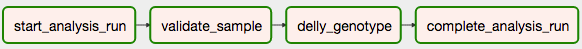
\includegraphics[width=\textwidth]{butler_delly_workflow}
\centering
\caption {Structure of the Butler Delly workflow}
\label{fig:butler_delly_workflow}
\end{figure}

This workflow has a familiar linear structure with the bulk of the work being done inside the delly\_genotype task. Because Delly knows how to work with and output compressed VCF files there is no need to compress and generate indexes like with freebayes. This makes the task code simpler (Listing \ref{lst:run_delly}).


After extracting the necessary configuration parameters and setting up the delly execution command, once delly execution finishes, the resulting call-set is copied over to its final location. Control over program behaviour is mostly exercised at the analysis level, where program flags are typically indicated (Listing \ref{lst:delly_analysis})

\section{Experimental Runs}

Between January and October 2016 Butler has been used extensively to facilitate a number of large scale cancer genomics analyses on behalf of the Germline Working Group of the Pan Cancer Analysis of Whole Genomes Project. The input to these analyses has been a 725 TB data-set of 2834 cancer patients' sequenced DNA samples, and the outputs have been a number of call-sets identifying and genotyping various classes of germline variants in the form of VCF files. All of the computations have been performed on the EMBL/EBI Embassy Cloud - a 1500 core, 6TB of RAM, 1PB of storage, academic cloud running Openstack.

In this section we describe the technical details and characteristics of these experimental runs to establish a measure of Butler's effectiveness in real-life scenarios.

\subsection{Freebayes Common Variant Genotyping}

The Common Variant Genotyping analysis refers to the genotyping within the PCAWG cohort the genomic variants that occur with at least 1\% Minor Allele Frequency (MAF) within the 1000 Genomes Project's\autocite{10002012integrated} cohort. This site list consists of ~12 million variants that need to be genotyped for each patient - thus requiring genotyping at 34 billion sites.

To accomplish this task we utilize the Butler freebayes workflow in genotyping mode, supplying the following configurations:

\captionof{listing}{Butler Freebayes Workflow analysis configuration for common variants genotyping.\label{lst:analysis_1_percent_maf}}
\begin{minted}
[
breaklines=true,
breakanywhere=true,
fontsize=\footnotesize,
linenos,
frame=lines,
framesep=2mm,
baselinestretch=1.2
]
{json}
{
	"variants_location": {
		"1": "/1000GP_maf_0.01/ALL.chr1.vcf.gz",
	        "2": "/1000GP_maf_0.01/ALL.chr2.vcf.gz",
	        "3": "/1000GP_maf_0.01/ALL.chr3.vcf.gz",
	        "4": "/1000GP_maf_0.01/ALL.chr4.vcf.gz",
	        "5": "/1000GP_maf_0.01/ALL.chr5.vcf.gz",
	        "6": "/1000GP_maf_0.01/ALL.chr6.vcf.gz",
	        "7": "/1000GP_maf_0.01/ALL.chr7.vcf.gz",
	        "8": "/1000GP_maf_0.01/ALL.chr8.vcf.gz",
	        "9": "/1000GP_maf_0.01/ALL.chr9.vcf.gz",
	        "10": "/1000GP_maf_0.01/ALL.chr10.vcf.gz",
	        "11": "/1000GP_maf_0.01/ALL.chr11.vcf.gz",
	        "12": "/1000GP_maf_0.01/ALL.chr12.vcf.gz",
	        "13": "/1000GP_maf_0.01/ALL.chr13.vcf.gz",
	        "14": "/1000GP_maf_0.01/ALL.chr14.vcf.gz",
	        "15": "/1000GP_maf_0.01/ALL.chr15.vcf.gz",
	        "16": "/1000GP_maf_0.01/ALL.chr16.vcf.gz",
	        "17": "/1000GP_maf_0.01/ALL.chr17.vcf.gz",
	        "18": "/1000GP_maf_0.01/ALL.chr18.vcf.gz",
	        "19": "/1000GP_maf_0.01/ALL.chr19.vcf.gz",
	        "20": "/1000GP_maf_0.01/ALL.chr20.vcf.gz",
	        "21": "/1000GP_maf_0.01/ALL.chr21.vcf.gz",
	        "22": "/1000GP_maf_0.01/ALL.chr22.vcf.gz"
	},
	"results_base_path": "/shared/data/results/regenotype_1_percent_maf/",
	"results_local_path": "/tmp/regenotype_1_percent_maf/",
	"freebayes": {
		"mode": "regenotyping",
		"flags": "-l"
	}
}
\end{minted}

Figure \ref{fig:freebayes_1_percent_maf_genotyping} shows a distribution of job runtimes (in minutes) separated by chromosome. The mean runtime is highly correlated with chromosome length (and consequently number of variants), with a Pearson correlation of 0.92.

\begin{figure}[H]
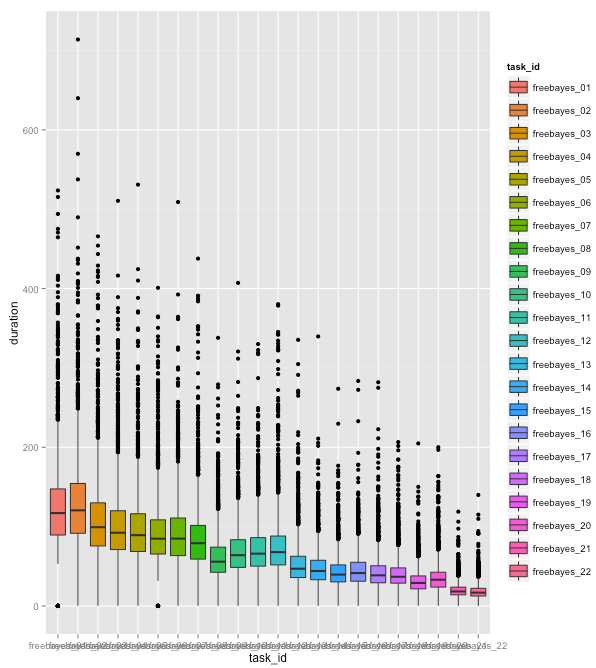
\includegraphics[scale=0.6]{freebayes_1_percent_maf_genotyping}
\centering
\caption {Runtimes of freebayes genotyping on the 1\% MAF site-list.}
\label{fig:freebayes_1_percent_maf_genotyping}
\end{figure}

Overall 130,152 compute hours were used to complete 70,850 workflow tasks for this analysis with an additional 2688 CPU hours used for cluster management overhead. Thus, management overhead accounted for ~2\% of the overall computational resource costs for this analysis. Utilizing 1000 cores this analysis took less than 6 days to complete.

\subsection{Freebayes Variant Discovery}
\subsection{Freebayes Variant Genotyping}

Using the site-list of 60 million variants obtained from the Freebayes Variant Discovery analysis we used the Butler Freebayes Workflow in genotyping mode to calculate genotypes at ~170 billion genomic positions. 76,518 tasks workflow tasks were completed utilizing 302,071 CPU hours over the course of the analysis (~10 days wall time), of which 5,040 CPU hours were cluster management overhead, accounting for 1.6\% of total resource utilization. Figure  \ref{fig:freebayes_discovery_regenotype_task_durations} demonstrates the distribution of task durations by chromosome.

\begin{figure}[H]
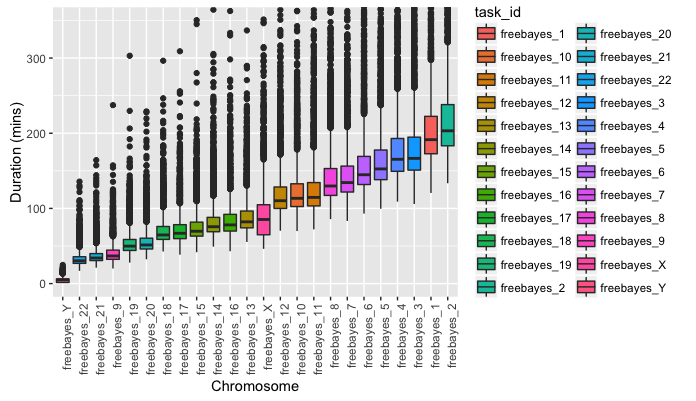
\includegraphics[width=\textwidth]{freebayes_discovery_regenotype_task_durations}
\centering
\caption {Runtimes of freebayes regenotyping on the freebayes discovery call-set.}
\label{fig:freebayes_discovery_regenotype_task_durations}
\end{figure}

Figure \ref{fig:freebayes_discovery_regenotype_task_duration_densities} provides a density-based view of task durations split by chromosome. We observe that durations in each case tend to fall about some mean, dependent on chromosome length (Pearson's r = 0.925), with variance also decreasing with chromosome length (r = 0.94). In each case there is a considerable right tail of duration outcomes, with the maximum duration for each chromosome occurring on average 11.7 standard deviations from the mean.

\begin{figure}[H]
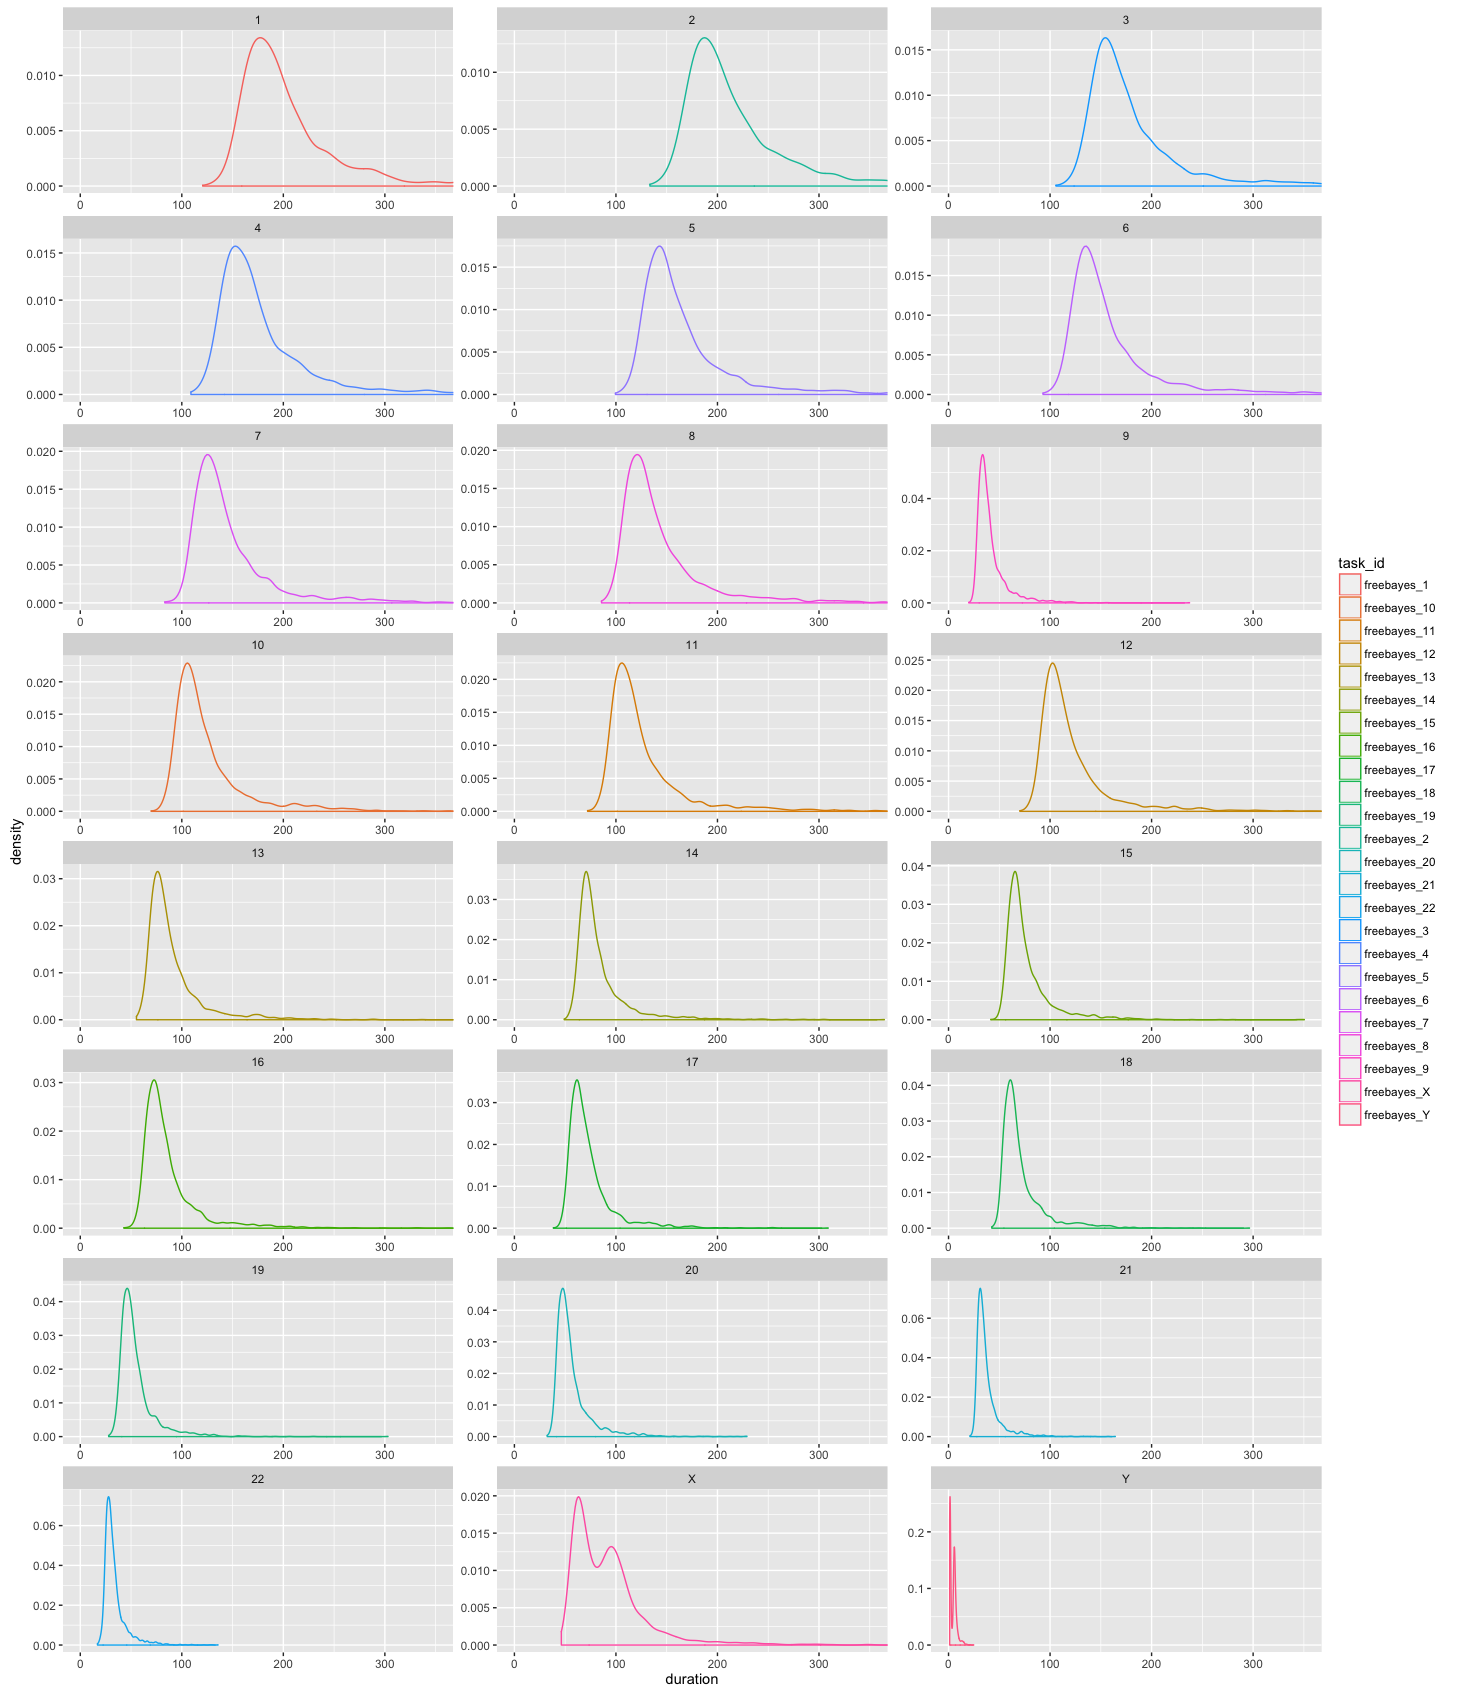
\includegraphics[width=\textwidth]{freebayes_discovery_regenotype_task_duration_densities}
\centering
\caption {Task duration distributions by chromosome.}
\label{fig:freebayes_discovery_regenotype_task_duration_densities}
\end{figure}

Figure \ref{fig:freebayes_discovery_regenotype_cluster_load} shows a view of the cluster load during the analysis execution. Here we see that overall the load has been stable, with a few sporadic spikes (5/25, 5/28, 5/29). On the other hand we see that the load is not uniform across the cluster with some machines not fully utilized. This is clear from the CPU utilization panel, where the majority of the VMs are at 100\% CPU utilization throughout the analysis execution, but several machines appear to be stable at utilization levels between 50\% and 90\%.

\begin{figure}[H]
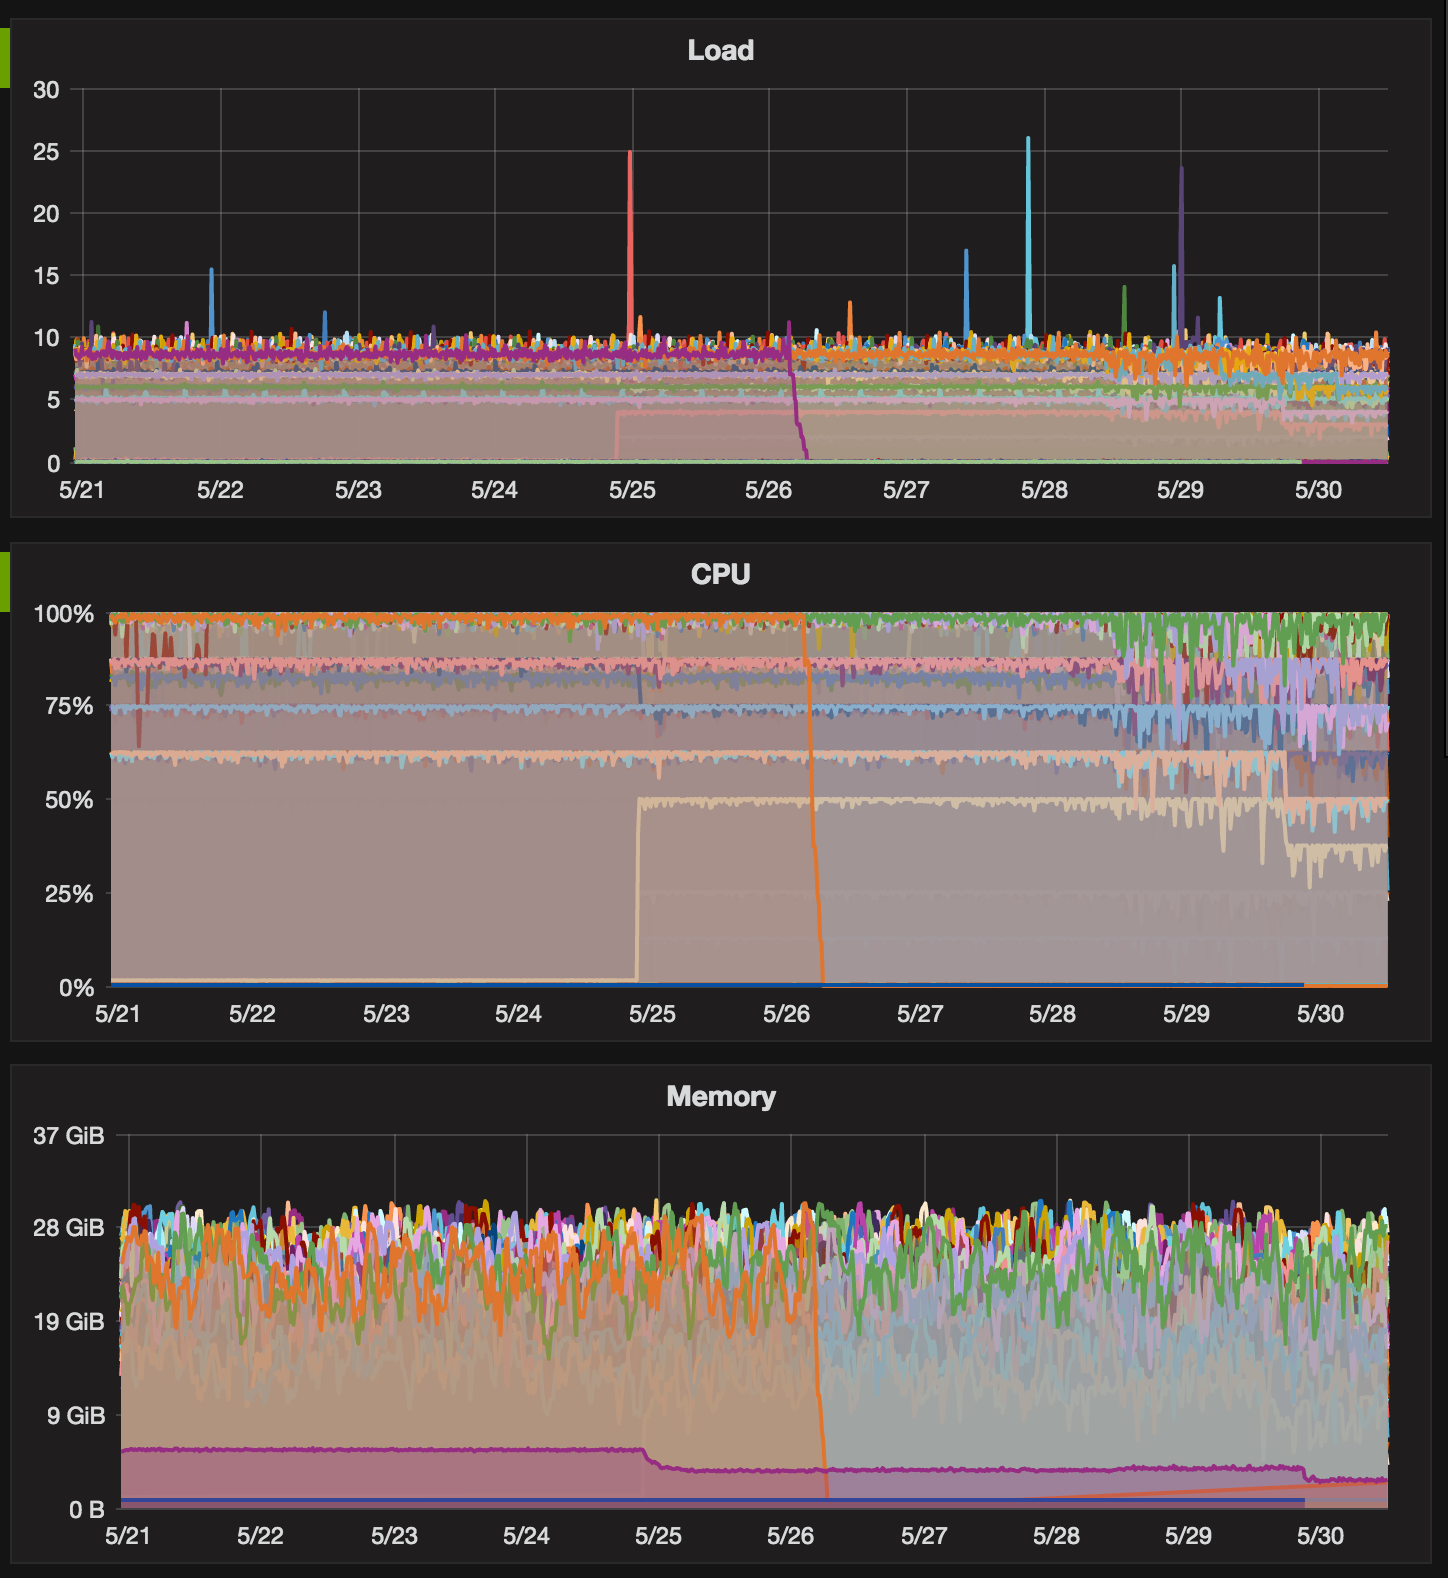
\includegraphics[width=\textwidth]{freebayes_discovery_regenotype_cluster_load}
\centering
\caption {Cluster resource utilization during the regenotyping analysis.}
\label{fig:freebayes_discovery_regenotype_cluster_load}
\end{figure}

\subsection{Delly Full Variant Genotyping}

The analysis of Delly Structural Variant Calling has been split into two parts - genotyping of germline deletions, and genotyping of germline duplications. We consider each in turn.


\subsubsection{Deletions Genotyping}
The deletions analysis used the following analysis configuration:

\captionof{listing}{Butler Delly Workflow analysis configuration for deletions genotyping.\label{lst:delly_analysis_dels}}
\begin{minted}
[
breaklines=true,
breakanywhere=true,
fontsize=\footnotesize,
linenos,
frame=lines,
framesep=2mm,
baselinestretch=1.2
]
{json}
{
	"variants_location": "/shared/data/samples/vcf/delly_deletion_sites/del.sites.bcf",
	"results_base_path": "/shared/data/results/delly_germline_deletions_14_07_2016/",
	"results_local_path": "/tmp/delly_germline_deletions/",
	"variants_type": "DEL"
	
}
\end{minted}
244,889 deletions were evaluated across 5668 samples (tumour and normal) for a total of 1,388,030,852 genomic sites genotyped. Overall wall-time was 13 days, utilizing 265,200 CPU hours with 6240 CPU hours used for cluster management overhead - an overhead of 2.2\%. 

Figure \ref{fig:delly_deletion_durations} shows a histogram of genotyping (sample level) jobs.

\begin{figure}[H]
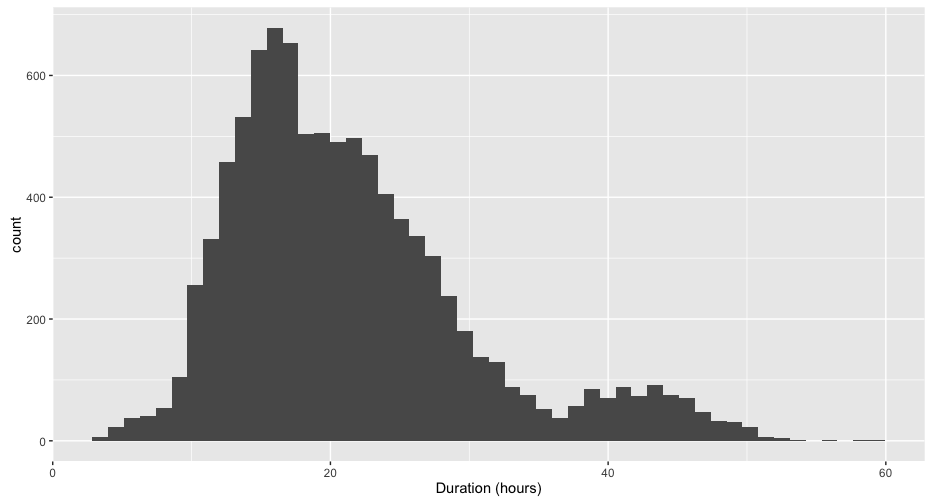
\includegraphics[width=\textwidth]{delly_deletion_durations}
\centering
\caption {Durations of deletion genotyping tasks by sample.}
\label{fig:delly_deletion_durations}
\end{figure}

Table \ref{tab:delly_deletion_summary_stats} shows the summary statistics of job durations.

\begin{table}[H]
\caption {Summary statistics of delly deletion genotyping job durations} \label{tab:delly_deletion_summary_stats}
\centering
\begin{tabular}{lrrrrr}
  \hline
 task\_id & mean & median & sd & min & max \\ 
  \hline
delly\_genotype & 21.48 & 19.70 & 8.89 & 3.35 & 59.30 \\ 
   \hline
\end{tabular}
\end{table}

Figure \ref{fig:delly_deletion_genotyping} shows the overall cluster load during the deletion genotyping analysis. During this analysis there were several periods during which the Workflow Scheduler failed and the job queue ran out of tasks. These periods can be seen as dips on the Load, CPU, and Memory metrics' graphs. 

\begin{figure}[H]
\includegraphics[width=\textwidth]{delly_deletion_regenotyping}
\centering
\caption {Cluster performance during the deletion genotyping analysis.}
\label{fig:delly_deletion_genotyping}
\end{figure}

\subsubsection{Duplications Genotyping}

The duplications analysis used the following configuration:

\captionof{listing}{Butler Delly Workflow analysis configuration for duplications genotyping.\label{lst:analysis_delly_dups}}
\begin{minted}
[
breaklines=true,
breakanywhere=true,
fontsize=\footnotesize,
linenos,
frame=lines,
framesep=2mm,
baselinestretch=1.2
]
{json}
{
	"variants_location": "/shared/data/samples/vcf/delly_deletion_sites/dup.sites.bcf",
	"results_base_path": "/shared/data/results/delly_germline_dups_05_09_2016/",
	"results_local_path": "/tmp/delly_germline_dups/",
	"variants_type": "DUP"
	
}
\end{minted}

Overall 217,433 duplications were genotyped for each sample, across 5668 samples for a total of 1,232,410,244 genomic variants genotyped. The wall-time for this analysis was only 4.5 days, utilizing 151,200 CPU hours during this time, with a management overhead of 2160 hours, for a total overhead of 1.4\%. The comparatively lower cluster management overhead has been accomplished by scaling up the cluster to 1400 cores without the need for more management resources.

Figure \ref{fig:delly_duplication_durations} shows a histogram of genotyping job durations.

\begin{figure}[H]
\includegraphics[width=\textwidth]{delly_duplication_durations}
\centering
\caption {Durations of duplication genotyping tasks by sample.}
\label{fig:delly_duplication_durations}
\end{figure}

Table \ref{tab:delly_duplication_summary_stats} provides summary statistics of the same data.

\begin{table}[H]
\caption {Summary statistics of delly duplication genotyping job durations} \label{tab:delly_duplication_summary_stats}
\centering
\begin{tabular}{rlrrrrr}
  \hline
 & task\_id & mean & median & sd & min & max \\ 
  \hline
1 & delly\_genotype & 14.27 & 12.32 & 8.80 & 2.15 & 52.19 \\ 
   \hline
\end{tabular}
\end{table}

Figure \ref{fig:delly_duplication_regenotyping} shows a measurement of cluster performance during the duplication genotyping analysis. This analysis appears to have run very smoothly, with two tranches of data - the normal genomes, and the tumour genomes closely following each other and exhibiting stable Load and Memory performance, and a CPU load profile that is, although spiky, is normal for Delly execution.

\begin{figure}[H]
\includegraphics[width=\textwidth]{delly_duplication_regenotyping}
\centering
\caption {Cluster performance during the duplication genotyping analysis.}
\label{fig:delly_duplication_regenotyping}
\end{figure}

Carrying out large-scale scientific analyses in the cloud has its own distinct set of challenges from other types of scientific analyses. Throughout this work we have established four key areas of concerns that need to be met in order to facilitate the performance of such analyses by the end user - Provisioning, Configuration Management, Workflow, and Operations Management. We have built the Butler framework to utilize existing robust open-source components where possible to fulfill the detailed requirements in the four areas thus described.

\section{System Design Recap}
Butler uses the Terraform provisioning tool in order to be able to create arbitrarily complex clusters in a cloud-agnostic manner, including artefacts such as Virtual Machines, networks, and security rules. We have used this capability to create test clusters on Amazon Web Services as well as rapidly creating and destroying production clusters on the EMBL/EBI's Embassy Cloud of over 180 VMs and associated network and security infrastructure, as necessary. 

Butler uses the Saltstack framework to enable scalable and platform-agnostic capabilities including the installation and run-time configuration of software and servers. We have used these capabilities to develop configuration profiles for over 30 different software packages that are used within Butler, both to configure Butler itself as well as configuring the scientific software required by particular workflows. The packages configured and installed by Butler are as varied as - PostgreSQL Server, RabbitMQ, GlusterFS, Influxdb, Elasticsearch, dnsmasq, Collectd, Freebayes, Delly, Samtools, and others. The role-based configuration model that have been put in place allows the user to simply create a new Virtual Machine and give it appropriate roles, when the machine communicates with the Salt Master it will be configured fully to the state prescribed by its roles and able to carry out useful work within minutes.

Butler utilizes a scalable and robust Airflow framework for its workflows. Because Airflow workflows are Python programs the users have all the power and flexibility of Python and its extended libraries at their disposal. The fact that each workflow task is a separate entity that can run on any worker machine in the cluster allows Airflow to be extremely scalable. 

To enable provenance tracking of scientific analyses we implemented a \mintinline{python}{tracker} module in Python that models the relationship between Workflows, Analyses, and Analysis Runs, the latter being the main execution unit of a workflow associated with a particular analysis and data sample. Using a PostgreSQL database we keep track of Analysis Run state transitions and execution history.

To further facilitate workflow configurability we implemented a hierarchical configuration mechanism using JSON-formatted configuration files that are specified at three levels of granularity and resolved into an \emph{effective} configuration at runtime. The JSON configurations form part of the provenance trail for an analysis and are stored in a PostgreSQL database which has native support for this data type, including query language extensions\autocite{lerner2014forge}.

Butler's Operations Management framework relies on two complementary systems - metrics, and logs. The metrics collection system is an agglomeration of tools that work together to harvest over 50 health metrics from each host and into a time-series database wherefrom a dashboarding engine presents the information in a series of dashboards. The log collection system similarly harvests application and server logs, filtering them down to extract useful information and storing it in an Elasticsearch index. Log information is then visualized in a set of separate dashboards. The two data collection and visualization systems provide the user with information at two granularity levels - the metrics system is more coarse-grained and gives a VM-level view of the health of the system, while the log system provides an application level view with a finer grained resolution of the events that are occurring at any given time. Together, these two systems allow the user to have very clear visibility into the overall system health and detect any issues, whether they be individual machine or application crashes, or wider systemic events like network bottlenecks or outages.

\section{Validation and Conclusion}
We have deployed Butler in a production setting at the EMBL/EBI's Embassy Cloud in a configuration that utilizes 1500 CPUs, 6 TB RAM, 1 PB of Isilon storage accessed over NFS, and 40 TB of block-storage. Furthermore, we have built a series of workflows that facilitate the large-scale cancer genomics analyses carried out by the Germline Working Group of the Pan Cancer Analysis of Whole Genomes project, including:

\begin{itemize}
\item Germline SNV discovery
\item Germline SNV joint-genotyping
\item Germline SV genotyping
\item Variant Filtration
\item Sample submission
\end{itemize}

Using these workflows wSe have carried out a number of analyses on a 725TB data set of 2834 cancer patients' DNA samples consuming a total of 546,552 CPU hours. Each analysis took no longer than two weeks to complete and utilized only 1.5\% - 2.2\% of the overall compute capacity for management overhead. On several occasions we were able detect large scale cluster instability and program crashes utilizing the Operational Management system and take corrective action with a minimal impact on overall cluster productivity.

Subsequent to the success of these analyses several research groups from the European Bioinformatics Institute, Ontario Institute for Cancer Research, Francis Crick Institute, and the Centre for Genomic Regulation have expressed their interest in utilizing Butler for their own large scale analyses in the cloud.

Based on the adherence of the Butler design and implementation to the stated set of requirements, and sustained successful production operation in a large scale deployment on a multitude of scientific analyses of significant scope and size, we conclude that the Butler framework is an effective tool for large scale scientific workflow management in the cloud.

\section{Future Direction}

Butler has been created to facilitate scientific analyses at scale and we have demonstrated that it is able to successfully perform at the level required for today's big data initiatives in the genomics domain. There are projects on the horizon, however, that are one to two orders of magnitude larger than the current biggest projects, these include the UK's 100,000 Genomes Project\autocite{marx2015dna}, and the US Precision Medicine Initiative\autocite{collins2015new} (with up to 1,000,000 genomes). This means that in order to not have to proportionately increase the timeline for theses projects the computational infrastructure will have to be scaled up instead. It is thus imperative for Butler's continued relevance to be able to ascertain the framework's performance level at 1 or 2 orders of magnitude larger than the current 1500 core empirically obtained result. The most immediate opportunity to do so will come up in 2017 when the EMBL/EBI's Embassy Cloud will be upgraded to 5000 CPU cores and Butler has been invited to take part in the stress-testing of the upgraded cloud. 

It is important to grow the library of workflows that are readily available for the Butler system to make the framework more appealing to new users. The Technical Working Group of the PCAWG project is in the process of migrating all of the main computational pipelines that have been used in the project into Docker\autocite{merkel2014docker} containers. Although the workflows that have been developed for the Germline Working Group have not yet been ported to Docker, Airflow, the workflow system underlying Butler has support for running Docker containers. Thus, a key next step for growing the library of Butler workflows lies in the adaptation of the core PCAWG workflows to be able to easily run them on a Butler instance. This would allow Butler to offer a comprehensive set of next generation sequencing workflows that are used for cancer genomics analysis.

Deploying Butler to a larger variety of environments will confirm the multi-cloud purpose of the framework and allow for the development of a richer set of configuration and provisioning profiles, as necessitated by the differences between deployment environments. On the basis of the already completed analyses for the PCAWG Germline Working Group, the Butler framework has also been selected to help deliver the science demonstrator work packet of the European Open Science Cloud Pilot\autocite{European_Open_Science_Cloud_2016} initiative that is launching in 2017. Additionally, de.NBI - The German Network for Bioinformatics Infrastructure\autocite{denbi_2016-10-31} which is working to establish a German academic cloud computing environment for bioinformatics research will be using Butler to deliver a number of new bioinformatics pipelines on its cloud in 2017.

Thus, over the course of the next 12 months the focus of Butler development will be on supporting improved scalability, developing a richer set of computational pipelines and operating in a number of new cloud computing environments. These steps should result in a more robust, feature rich, and useful tool.

  






\chapter{The Rheos Framework} \label{ch:rheos_framework}
%In this chapter we describe a software framework called Rheos, which demonstrates an approach for reasoning about large genomic datasets utilizing concepts of service-orientation and data streaming in contrast with traditional genomic data analysis frameworks\autocite{depristo2011framework} that take a procedural batch-based approach. Rheos' focus on service-orientation and streaming allow the users to make active tradeoff decisions between analysis time, cost, and quality as well as setting up precise operational Service Level Agreements, both between Rheos components, and between Rheos and external systems, as we describe in detail below.

\section{General Framework Design}

As already discussed in Chapters \ref{ch:introduction} and \ref{ch:background}, the general problem consists of collecting DNA samples from a population of individuals under study, sequencing these samples using Next Generation Sequencing techniques, identifying the mutations that are present, annotating their functional impact and utilizing the obtained data in a downstream data analysis with research or clinical decision-making goals. While there is a great variety of possible downstream analyses that may be performed depending on the individual goals of the analyst, there is a fairly well established set of steps for processing of the raw NGS data into a set of annotated variants, and it is these steps that we target with this work. The typical approach that is in widespread use today is to collect a batch of samples and then process each sample individually with a sequence of individual tools, that may be described via a higher-level workflow construct (such as in Figure \ref{fig:gatk_best_practices}, or using a framework like Butler, as described in Chapters \ref{ch:butler_architecture}, \ref{ch:butler_implementation}). There are, however, a number of factors that leave room for improvement in this model. These improvements lie along a set of dimensions that we describe briefly in the Introduction via a utility function $U_i = C_i + T_i + A_i$ for sample $i \in [1,N_s]$  that needs to be optimized, and that we describe in more detail here.

We use the following definitions throughout the text:

\begin{table}[!ht]
    \caption{Rheos common definitions}
    \label{tab:rheos_notation}
    {\begin{tabular}{lp{7cm}}
    \toprule
    Symbol & Description \\
    \midrule
    $N_p$ & Number of people \\
    $P = \{p_i : i \in [1,N_p]\}$ & Set of individuals under study \\
    $N_s$ & Number of samples \\
    $S = \{s_i : i \in [1,N_s]\}$ & Set of sequenced DNA samples. Each individual can have one or more samples. \\
    $A_i $ & Accuracy score of analysis for sample $i$ (precise definition of Accuracy TBD) \\
    $C_i = c_{g_i} + c_{s_i} + c_{a_i} + c_{r_i}$ & Cost score of data generation, storage, analysis, and retrieval respectively \\
    $T_i$ & Time score to process sample $i$ \\
    $U_i = C_i + T_i + A_i$ & A utility function for individual $i$ that penalizes high cost, high processing time, and low accuracy\\
    $U = \sum_{i=1}^{N_s} U_i$ & Overall utility of processing $N_s$ samples through Rheos.\\
    \bottomrule
    \end{tabular}}
\end{table}


\section{Data Streaming Architecture}
\label{sec:rheos_streaming_architecture}

The overall technical architecture of the Rheos system is set up as a Service Oriented Architecture (SOA)\autocite{shaw1996software} which is an information system architecture paradigm where the overall problem that the system is trying to solve is broken down into a collection of loosely-coupled components called services. Each service has a well defined interface of inputs that it accepts and outputs that it produces. Services can be combined and orchestrated together to produce the overall desired output for the system. A key distinguishing feature of this architectural approach is that each service can be individually optimized to fulfill its contract most efficiently helping break down some of the performance limitations brought about by the necessity to simultaneously tackle competing constraints in more monolithic information system designs. Additionally, within a services framework, the dependencies between separate services can be negotiated not only in terms of service interfaces, but also in terms Service Level Agreements which constitute Quality of Service promises made by one service to its dependents\autocite{ingham2000constructing}. Because it is unlikely that a service designer will be able to accurately foresee all of the demands that will be placed on a service during its lifetime the SLAs provide a valuable feedback framework through which the service can be evaluated as it operates in production, as well as serving as a basis for negotiating evolving requirements between dependent services.

While general web services can support any data processing paradigm, in the Rheos framework we adopt a data streaming approach\autocite{babcock2002models}. In this approach we assume that the input to any service is a randomly ordered sequence of messages $M = {m_1, m_2, ....}$ where each message represents a fact about the underlying domain that the service reasons over, as well as some metadata, including an identifier, and a variety of timestamps of interest. The content of each message may provide a datum, such as the measurement of a quantity of interest, or signal that a particular event has taken place. It is in general assumed that the data stream is infinite in size, that messages may arrive out of order, and that any message that is placed in the stream is observed at most once, and may, in fact, never be observed. Messages are typically not sent directly from one service to another, instead the transfer of messages is mediated by a queuing system using a publish-subscribe\autocite{eugster2003many} model. Under this model each queue acts as a \emph{topic}. Message producers can publish data to the topic, and message consumers subscribe to receive messages from the topic. A message is consumed from the queue only after all of the subscribed consumers have seen it. End users retrieve information from the system via a set of User Interfaces that support both push (notifications) and pull (querying) models of data retrieval. A more detailed description of the architectural aspects of the system follows:

\subsection{Service-Oriented Data Streaming Model}
\label{sec:rheos_data_streaming_model}


A data stream $M_{s,d} = {m_1, m_2, ....}$ is a sequence of datagrams transmitted over the network with the following properties:

\begin{itemize}
    \item The stream has a source $s$ and a destination $d$.
    \item A message $m$ in the stream is a tuple of the form $(header, payload)$, where:
    \begin{itemize}
        \item $header$ is a tuple of the form $(id, \dots)$ that holds at minimum a unique identifier $id$ for messages, and may hold additional metadata.
        \item $payload$ is an arbitrary data structure that holds the informational content of the message. 
    \end{itemize}
    \item $|M| = \infty$ by assumption.
    \item Messages may not arrive at destination $d$ in the same order that they were sent from source $s$.
    \item If $t_{i,s}$ is the time message $m_i$ leaves the source $s$ and $t_{i,d}$ is the time of arrival at destination $d$, then $\sup_i \{t_{i,d} - t_{i,s}\} = \infty$, i.e. a given sent message may never arrive at its destination.
\end{itemize}

A service $S = \{o_i\}$ is a collection of operations $o_i$ that act on one or more input data streams $\{M_i\}$ to produce one or more transformed output data streams $\{M_j\}$. Specifically:

An operation $O$ is a tuple of the form:

\begin{equation}
\label{eq:service_opertaion_equation}
O = (i,o,p,f)
\end{equation} 
where:
\begin{itemize} 
    \item $i = \{M_j, j \in [0, K]\}$ is a set of $K \ge 0$ input data streams.
    \item $o = \{M'_j, j \in [0, L]\}$ is a set of $L \ge 0$ output data streams.
    \item $f:M^K \mapsto M'^L$ is a transformation function that produces messages $m'$ in the output streams based on messages $m$ observed in the input streams.
    \item $p = \{p_i\}$ is a set of potentially optional query parameters.  
\end{itemize}

There are several distinct categories of operations that a service can perform on a set of input streams. We describe these here:

\paragraph{Windowing Function} - Service $S$ observes a sliding window, which is a sample of size $n$ of messages from stream $M_i$ and computes a summary statistic (see Figure \ref{fig:stream_window_function}) over the sample which is meant to be an approximation of the corresponding population parameter.

\begin{figure}[H]
\includegraphics[scale=0.6]{stream_window_function}
\centering
\caption {Service S computes a summary statistic over a window of messages from stream $M$}
\label{fig:stream_window_function}
\end{figure}
 
\paragraph{Decorator Function} - Service $S$ observes messages $m_i$ and applies a function that augments (decorates) each message with additional attributes (see Figure \ref{fig:stream_decorator_function}) producing augmented messages $m_o$ as output.

\begin{figure}[H]
\includegraphics[scale=0.6]{stream_decorator_function}
\centering
\caption {Service S augments messages from $M$ with an additional set of attributes.}
\label{fig:stream_decorator_function}
\end{figure}

\paragraph{Filter Function} - Service $S$ observes messages $m_i$ and applies a function $f:M\mapsto\{True,False\}$ that evaluates to a boolean value (see Figure \ref{fig:stream_decorator_function}). Only messages that map to $True$ are emitted as output.

\begin{figure}[H]
\includegraphics[scale=0.6]{stream_filter_function}
\centering
\caption {Service S filters messages from input stream $M$ and only allows through those that pass the filtering condition.}
\label{fig:stream_filter_function}
\end{figure}

\paragraph{Aggregator Function} - Service $S$ observes messages from $N$ different streams $\{M_j: j \in [1,N]\}$ and applies a function $f:M_i^N \mapsto M_o$ that aggregates messages from these streams to produce its output (see Figure \ref{fig:stream_aggregator_function}). Because aggregation happens over groups of messages that may not all arrive at the same time the service $S$ requires a mechanism for keeping local state so that it can accumulate messages that have already arrived while waiting for those that are necessary to compute $f$ yet have not been observed. The statefulness requirement of this type of service places an extra level of complexity (related to state-management and request routing) as well as inherent scalability limitations compared to stateless services\autocite{oppenheimer2002architecture}.

\begin{figure}[H]
\includegraphics[scale=0.6]{stream_aggregator_function}
\centering
\caption {Service S integrates messages from multiple input streams $M_i$ to produce an aggregated output stream $M_o$ via $f$.}
\label{fig:stream_aggregator_function}
\end{figure}


\paragraph{Local State Aggregator Function} - Service $S$ observes an input stream $M_i$ which it integrates with a local (non-stream) queryable data store (see Figure \ref{fig:stream_local_state_aggregator_function}). Messages $m_i$ are integrated with query results $q_i$ to produce an output stream $M_i$. This type of service also requires management of state and scalability concerns similar to the Aggregator service, especially when the local data store is itself distributed. 

\begin{figure}[H]
\includegraphics[scale=0.6]{stream_local_state_aggregator_function}
\centering
\caption {Service S aggregates $m_i$ with query results $q_i$ obtained from a local data store.}
\label{fig:stream_local_state_aggregator_function}
\end{figure}


\paragraph{Persistence Function} - Service $S$ observes messages $m_i$ and is responsible for persisting them to a data store where their contents can later be queried (see Figure \ref{fig:stream_persistence_function}). Although persistence of data to, and subsequent querying of data from, a store, such as a database, are comparatively more expensive operations than immediate reasoning over a live data stream, such mechanisms are necessary for situations where data may need to be accessed multiple times, or where data may need to be retained for audit purposes.

\begin{figure}[H]
\includegraphics[scale=0.6]{stream_persistence_function}
\centering
\caption {Service $S$ processes messages $m_i$ into persistent storage. The output stream $M_o$ contains persistence confirmation and error events.}
\label{fig:stream_persistence_function}
\end{figure}

\paragraph{Query Function} - Service $S$ observes a stream of queries $Q_i$. The queries are fulfilled against a data store $D$ and the results emitted via the output stream $M_o$.

\begin{figure}[H]
\includegraphics[scale=0.6]{stream_query_function}
\centering
\caption {Service S filters messages from input stream $M$ and only allows through those that pass the filtering condition.}
\label{fig:stream_query_function}
\end{figure}

The basic operations above can be combined to produce arbitrarily complex logic on data streams.

One of the key advantages of a service-oriented approach is that, because services are typically constantly executing, it naturally lends itself to an examination of the system's runtime characteristics. This applies to both service-internal characteristics that are related to each operation a service performs, as well as to external characteristics that relate to the contracts a service establishes with its dependencies. We consider both of these.

For each given operation $o_i \in S$ it is instrumental to understand the resource requirements of the operation on typical inputs and limiting factors that affect the efficiency with which the operation can be performed by $S$. Of particular interest are the per-operation profiles of:

\begin{itemize}
    \item CPU utilization
    \item RAM
    \item Secondary storage
    \item Network utilization
\end{itemize}

If $o_i$ is a long-running operation that takes multiple seconds to complete on average, a detailed distribution in time of each metric above may be necessary. If the operation can be completed at a sub-second rate then summary statistics (min, max, mean, median, inter-quartile range, 90th, and 99th percentiles) may be sufficient. This level of understanding is necessary in order to make sure that the service can adequately deal with the incoming message stream while the messages are first loaded into memory, since subsequent retrieval from secondary storage is several orders of magnitude slower and may cause further delays in processing. If $o_i$ is stateless, i.e. it does not require the storage and retrieval of any local state that depends on the content of each arriving message $m_j \in M_i$, then the service $S$ can be scaled "horizontally"\autocite{vaquero2011dynamically} with respect to $o_i$. Given that the performance-limiting condition of $o_i$ is known (CPU, memory, etc.), the ability of $S$ to efficiently deal with fluctuations in the rate of incoming messages $M_i$ can be successfully achieved simply by adding and removing servers that execute $S$ (see Figure \ref{fig:horizontal_vs_vertical_scaling}), which can be done automatically\autocite{mao2011auto}. If $o_i$ is stateful and requires access to databases, or predictable request routing via sessions, then horizontal scalability may not be possible and thus, detailed understanding of the performance profile and performance-limiting conditions of $o_i$ is even more important as vertical scaling of services is more expensive and challenging to accomplish, and may increase system complexity by necessitating data partitioning, for example\autocite{vaquero2011dynamically}.

\begin{figure}[H]
\includegraphics[scale=0.44]{horizontal_vs_vertical_scaling}
\centering
\caption {a) In horizontal scaling new servers are added and removed (dashed arrow) behind a load balancer as the rate of data stream $M_i$ fluctuates. b) In vertical scaling more powerful servers need to be launched (dashed arrow) to replace smaller servers (with potential service outage) when the rate of $M_i$ increases beyond capacity.}
\label{fig:horizontal_vs_vertical_scaling}
\end{figure}

Assume service $S$ implements operation $o$ supported by $n$ physical servers $V = \{v_j: j \in [1,n]\}$ by consuming a stream of incoming messages $M_i$. For a suitable time increment $t$, let $r_{M_i} = |M_i|/t$ be the incoming message arrival rate, and $r_{M_{o,j}} = |M_{o,j}|/t$ be the processing rate for server $v_j$. If $r_{M_i} > \sum_{j=1}^n r_{M_{o,j}}$, then $S$ will not be able to adequately process all of the incoming messages from $M_i$ and messages will either be lost or need to be backlogged while more servers are added to $S$ to deal with the incoming message rate. Since commissioning new servers takes considerable time and the timing and magnitude of increases in $r_{M_i}$ may be unpredictable, serious information loss may result if measures are not put in place to mitigate the message rate fluctuations. 

A queue is the mechanism that we put in place to address this concern (see Figure \ref{fig:queue}). A queue $Q$ is a message buffering system which consists of a set of $n$ "topics" $P = \{p_i: i \in [1,n]\}$, where each topic is a tuple of the form $p_i = (D_p,B_p,C_p)$. Here $D_p = \{d_i: i\in [1,k]\}$ is a set of $k$ data producers that put messages into $Q$, $B_p$ is a message buffer of max capacity $N_{max}$ dictated by underlying server hardware characteristics, containing a sequence of messages $\{m_t, m_{t-1},m_{t-2},....,m_1\}$ that are accessible in a Fist In First Out (FIFO) manner, and $C_p = \{c_i: i \in [1,l]\}$ is a set of $l$ consumers that are interested in observing messages from $p_i$.

\begin{figure}[H]
\includegraphics[scale=0.54]{queue}
\centering
\caption A queue $Q$ establishes a message buffer $B_p$ between a set of message producers $D_p$ and consumers $C_p$, for a given topic $p$.
\label{fig:queue}
\end{figure}

Messages arrive into a particular topic of $Q$ from all producers $D_p$, and are marked safe for deletion only when all of the subscribed consumers $C_p$ have observed a particular message. Thus, for topic $p_i$, the incoming message rate is $\displaystyle R_i = \sum_{j=1}^k r_{M_{o,j}}$ i.e. the sum of the message processing rates for all of the producers for this topic. The queue message processing rate $\displaystyle R_o = \min_{i \in [1,l]}\{r_{M_{o,i}}\}$ is the slowest message processing rate among all consumers. Assuming $R_i > R_o$ and that there are $N$ messages presently in $B_p$, there remains $t = \frac{N_{max} - N} {R_i - R_o}$ time before queue overflow occurs. The situation should then be remedied by allocating additional hardware to $Q$ or those services $S_i$ whose consumers are slowest, until the condition $R_o \ge R_i$ can be reliably maintained. If the queue does reach its maximum capacity overflow measures need to be put in place. Depending on the data stream in question data loss may or may not be acceptable. If data loss is acceptable then overflow messages can be simply discarded. If data loss is not acceptable then producers must block waiting for additional queue capacity to become available. This not only degrades performance locally, but can have a drastic effect on the entire system if the effects are allowed to percolate trough the complex distributed system. As message rates evolve through time with system load, the scheme above sets up a framework for flow control and hardware allocation within the architecture.

When designing a service-oriented system the interfaces of operations provided by the service are of utmost importance as they define the capabilities that the service offers to its clients. Of secondary, but also significant, importance is the set of Service-Level Agreements (SLAs)\autocite{wieder2011service} that a service advertises. These SLAs are a set of commitments that a service makes to its clients that describe the operational characteristics of the service, such as:

\begin{description}
    \item [Availability] - Guarantees related to the service uptime, maintenance outages, disaster recovery, etc.
    \item [Throughput] - The number of requests serviced per unit time.
    \item [Latency] - The delay between a request being sent and a response being received.
    \item [Abandonment Rate] - Proportion of requests that are never answered.
    \item [Error Rate] - Proportion of well-formed requests that result in an error.
\end{description}

Based on the SLAs that are advertised by a given service, the services that depend on it can make assumptions about expected runtime behavior, and take action when expectations are not met. Furthermore, when requirements evolve and features are added to or removed from a service, the impact on the advertised SLAs helps communicate the full effect of the changes. Lastly, the costs of operating a service are more clearly understood through the SLA framework, where improvements to a particular SLA metric, such as Transactions-Per-Minute (TPM) can be transparently traced to a corresponding increase in operational costs.

The set of services $\{S\}$ that communicate over data streams $\{M_{s,d}\}$, mediated by a set of queues $\{Q\}$ with a set of established SLAs $\{L_s\}$ together form the overall framework of Rheos that is used to tackle the challenges of large-scale genomic data processing in a manner the enables active tradeoffs between the competing constraints of cost, time, and accuracy. 

\section{Domain-specific Problems}

Having laid out the general data-streaming service-oriented architecture of Rheos in the previous section we now turn to a discussion of the set of actual domain-specific problems that need to be solved within the data-streaming paradigm in order to enable the comprehensive genomic characterization of large cohorts of samples within Rheos, as we have set out to do. We make use of the flow of data types from the most raw to the most refined (see Figure \ref{fig:ngs_flow}) to illustrate the challenges that need to be solved during transformation of the input data between each successive stage, first in summary form, and then in full detail, below.

\begin{figure}[H]
\includegraphics[scale=0.5]{ngs_flow}
\centering
\caption {The conceptual flow of data types within Rheos from the most raw - Sequencer Images, to the most refined - a set of Functionally Annotated Variants.}
\label{fig:ngs_flow}
\end{figure}
    
The most raw data type that is produced from a sequencing experiment is the set of raw image files generated by the sequencer. Although, conceptually, processing of the raw images could also be accomplished within Rheos, it is presently outside of the scope of this work. Instead, we assume the most basic data type to be raw sequencing reads, as found in a FASTQ\autocite{cock2009sanger} file. 

\begin{figure}[H]
\includegraphics[scale=0.40]{read_pair}
\centering
\caption {A read-pair that is aligned to the reference.}
\label{fig:rheos_read_pair}
\end{figure}

Each read is a tuple of the form:

\begin{equation}
\label{eq:raw_read_message}
r = (s\_id, r\_id, b, q, f_p)
\end{equation}

where:

\begin{itemize}
    \item $s\_id$ - is the sample ID, which is unique among all samples.
    \item $r\_id$ - is the read ID, which is unique among all reads for that sample.
    \item $b = \{b_1, b_2,.....,b_n\}$ - is the sequence of DNA bases, where $b_i \in \{A,C,G,T,N\}$.
    \item $q = \{q_1, q_2,....,q_n\}$ - is the set of PHRED-scaled base quality scores corresponding to the probability that the base has been called incorrectly. See discussion on FASTQ format in Section \ref{sec:bg_file_formats} for details.
    \item $f_p \in \{True, False\}$ - is a boolean flag indicating whether this read is the first read in a pair.
\end{itemize}

\subsection{Read QC Metrics}
\label{sec:main_body_read_qc_metrics}

Section \ref{sec:bg_raw_data_qc} of the Background chapter discusses various metrics of interest that are based on observations of read data and the tools that are used to collect them. Here we describe how to collect the most typical metrics in the streaming paradigm of Rheos. As before, there are per-read metrics such as Base Quality Distribution, and Adapter Sequence Presence, as well as per-sample metrics such as Average GC Content, Insert Distribution, Read Length Distribution, and others. The utility of these metrics is to be able to set up filters for low quality data as well as input for downstream variant-calling models (see Section \ref{sec:bg_germline_sv_calling} for example). 

Assume that we are observing a stream $M_{raw} = \{m_i: m_i = (header, payload)\}$ of read messages where the payload is a read $r$ as defined above. Under the assumptions of Section \ref{sec:rheos_streaming_architecture} we know that the number of elements in the stream is unbounded. We are able to straightforwardly calculate incremental estimates for metrics such as mean, variance, max, and min, but require more sophisticated structures for computing estimates of rank statistics such as median and other quantiles to maintain operations in bounded space. We use the following update rules for min, max, mean, and variance\autocite{welford1962note} calculations:

\begin{equation}
    \label{eq:stream_min}
    min_k(M) =  \begin{cases}
        m_k,& \text{if } m_k < min_{k-1}(M)\\
        min_{k-1}(M),& \text{otherwise}
    \end{cases}
\end{equation}

\begin{equation}
    \label{eq:stream_max}
    max_k(M) =  \begin{cases}
        m_k,& \text{if } m_k > max_{k-1}(M)\\
        max_{k-1}(M),& \text{otherwise}
    \end{cases}
\end{equation}

\begin{equation}
    \label{eq:stream_mean}
    \mu_k(M) =  \mu_{k-1}(M) + \frac {m_k - \mu_{k-1}} {k} 
\end{equation}

\begin{equation}
    \label{eq:stream_variance}
    \sigma_k^2(M) =  \frac{\sigma_{k-1}^2(M) + (m_k - \mu_{k-1}(M))(m_k - \mu_k(M))}{k-1} 
\end{equation}

In order to set up the mechanisms to answer quantile queries the following definitions are used\autocite{garofalakis2016data}:

\begin{itemize}
    \item Given a set $S$ of size $n$, and a quantile $\phi \in [0,1]$, return $v \in S$ whose rank in sorted $S$ is $\phi n$. 
    \item An $\epsilon$-approximate $\phi$-quantile is a value $v$ whose rank $r*(v) \in [n(\phi-\epsilon), n(\phi+\epsilon)]$.
    \item A quantile summary is $Q = {q_1,q_2,....,q_l: q_1\le q_2 \le \dots \le q_l, q_i \in S, i \in [1,l]}$ where each $q_i$ has rank at least $rmin_Q(q_i)$ and at most $rmax_Q(q_i)$ in $S$, and $rmax_Q(q_1) \le \epsilon|S|$, and $rmin_Q(q_l) \ge (1-\epsilon)|S|$.
    \item A quantile summary $Q(\epsilon)$ is $\epsilon$-approximate if it can be used to answer any quantile query with $\epsilon$-accuracy.
\end{itemize}

We use two approaches for computing quantile summaries, one due to Greenwald and Khanna\autocite{greenwald2001space} is able to compute the quantile summary using $O(log(\epsilon n)/\epsilon)$ space, and the other by Shrivastava et al.\autocite{shrivastava2004medians} computes the quantile summary in $O(log(M)/\epsilon)$ when the values are integers in range $[1,M]$. Both algorithms work for a scenario where one node sees all of the data in a stream, but can also be generalized to topologies where the stream is observed by multiple nodes in parallel. 

We provide several examples of QC queries of interest that are specified on a data stream:

\paragraph{Average Base Quality} -  As an assessment of the individual quality of each read we are interested in the average base quality so that we can filter out reads that are of low quality as a whole. We use a Decorator Function construct from Section \ref{sec:rheos_data_streaming_model}. 

\bgroup
\def\arraystretch{1.5}
\begin{table}[!ht]
    \caption{Definition of $q_{av}$ which computes average base quality for a read}
    \label{tab:op_average_base_quality}
    {\begin{tabular}{l|p{12cm}}
    \toprule
    Inputs & \hangindent=1em$M_{raw} = \{m_i: m_i = (header, payload)\}$ where $m.payload = r = (s\_id, r\_id, b, q, f_p)$ as in \ref{eq:raw_read_message}.\\
    \cline{2-2}
    Operation & $q_{av} = \frac{\sum_{i \in [1,|r|]} r.q_i}{|r|}$\\
    \cline{2-2}
    {Outputs} & \hangindent=1em$M_{out} = \{m_i: m_i = (header, payload)\}$ where $m.payload = r = (s\_id, r\_id, b, q, f_p, q_{av})$\\
    \bottomrule
    \end{tabular}}
\end{table}
\egroup


\paragraph{Base Quality Distribution} - The distribution of base quality scores per base position of a read and per sample are of interest to investigate the presence of systemic biases in base quality scores as a function of the position within the read.

\begin{figure}[H]
    \includegraphics[scale=0.35]{fastqc_per_base_quality}
    \centering
    \caption {Distribution of base qualities per read position, from https://www.bioinformatics.babraham.ac.uk/projects/fastqc. Large quality drop-off can be see towards the end of the read.}
    \label{fig:main_body_fastqc_per_base_quality}
\end{figure} 


Because PHRED-scaled quality scores are integers that fall in a fixed range $q \in [0,96]$ building quantile summaries using the q-gram\autocite{shrivastava2004medians} approach is the most space-efficient. Because base quality scores need to be aggregated over many reads and tracked for many samples, a service that implements this functionality needs to keep local state, and the operation to update the quantile summaries based on incoming reads follows the Local State Aggregator pattern from Section \ref{sec:rheos_data_streaming_model}. 

\bgroup
\def\arraystretch{1.5}
\begin{table}[!ht]
    \caption{Definition of $updateQuantileSummaries()$}
    \label{tab:op_update_quantile_summaries}
    {\begin{tabular}{l|p{12cm}}
    \toprule
    Inputs & \hangindent=1em$M_{raw} = \{m_i: m_i = (header, payload)\}$ where $m.payload = r = (s\_id, r\_id, b, q, f_p)$ as in \ref{eq:raw_read_message}. \\
    \cline{2-2}
    Operation & $updateQuantileSummaries(r)$\\
    \cline{2-2}
    {Outputs} & \hangindent=1em$M_{out} = \{m_i: m_i = (header, payload)\}$ where $m.payload = (s\_id, Q_{bqd})$.\\
    \bottomrule
    \end{tabular}}
\end{table}
\egroup

Since the local state required for storing the quantile summaries may not fit in memory and may need to be persisted to disk, updating the summaries may be too expensive to do for every single read that is observed in a read input stream. Instead, reads may be buffered into a set of reservoirs, triggering an update of the quantile summaries when the reservoir is full. The contents of the reservoir would then be purged and an updated set of quantile summaries $Q_s,{bqg} = \{q_i: i\in [1,max\_bases]\}$, where each $q_i$ is a quantile summary corresponding to the Base Quality Distribution at a particular read position, issued to the output stream (see Algorithm \ref{ag:update_quantile_summaries_bqd}).

\begin{algorithm2e}[h]
\DontPrintSemicolon
\footnotesize
    \textbf{Function} {\sc updateBQDQuantileSummaries}$(r)$
    \Begin {
        $reservoir \gets ${\sc getReservoir$(r.s\_id)$}\;
        $reservoir.${\sc addNewRead$(r)$}\;
        \If {$reservoir.isFull$}{
            $summaries \gets ${\sc getQuantileSummaries$(r.s\_id)$}\;
            \For{$read$ {\bf in} $reservoir$}{
                \For{$index,read.q$ {\bf in} $read$}{
                    {\sc updateQGram$(summaries[index], read.q)$} \tcp*{per \autocite{shrivastava2004medians}}\;
                }
            }
            {\sc purgeReservoir$(reservoir)$}\;
            {\sc outputQuantileSummary$(r.s\_id, summaries)$}\;
        }
    } 
\caption{Updating quantile summaries for Base Quality Distribution.}
\label{ag:update_quantile_summaries_bqd}
\end{algorithm2e}

\paragraph{Insert Size Distribution} - The insert size distribution is an important metric because it is not only indicative of the overall quality of a sample's data, but it is also used by structural variant calling to find read-pairs that map abnormally far apart (indicating a deletion), or abnormally close together (indicating an insertion). 

\begin{figure}[H]
    \includegraphics[scale=0.85]{insert_size_distribution}
    \centering
    \caption {Distribution of insert sizes from two ICGC pancreatic cancer patients DO35138 and DO22154.\autocite{stephens2016simulating}}
    \label{fig:insert_size_distribution}
\end{figure} 

Calculating this metric requires a stream of read-pairs, where both reads have been successfully mapped to the reference genome. Given a mapped read-pair $(r_1,r_2)$ where each read has a beginning coordinate $r.pos$ and an end coordinate $r.end$, the insert size is $l = r_2.end - r_1.pos$. We are interested in the mean, variance and quantiles of the insert size distribution. Because the insert length can be any size the quantile summary method of Greenwald and Khanna\autocite{greenwald2001space} is most appropriate for the quantiles. Read pairs are observed on the input stream and buffered in per-sample reservoirs. When a reservoir is full the read pairs are used to update and output an appropriate insert size distribution mean, variance, and quantile summary.

\bgroup
\def\arraystretch{1.5}
\begin{table}[!ht]
    \caption{Definition of $updateInsertSizeDistribution()$}
    \label{tab:op_update_insert_size_dist}
    {\begin{tabular}{l|p{12cm}}
    \toprule
    Inputs & \hangindent=1em$M_{pair} = \{m_i: m_i = (header, payload)\}$ where $m.payload = (r_1,r_2)$, and $r = (s\_id, r\_id, b, q, f_p)$ as in \ref{eq:raw_read_message}. \\
    \cline{2-2}
    Operation & $updateInsertSizeDistribution(s\_id,r_1, r_2)$\\
    \cline{2-2}
    {Outputs} & \hangindent=1em$M_{out} = \{m_i: m_i = (header, payload)\}$ where $m.payload = (s\_id, \mu_{isd}, \sigma_{isd}^2, Q_{isd})$.\\
    \bottomrule
    \end{tabular}}
\end{table}
\egroup

\begin{algorithm2e}[h]
    \DontPrintSemicolon
    \footnotesize
    \textbf{Function} {\sc updateInsertSizeDistribution}$(s\_id, r_1,r_2)$
    \Begin {
        $pairReservoir \gets ${\sc getReservoir$(s\_id)$}\;
        $pairReservoir.${\sc addNewReadPair$(r_1, r_2)$}\;
        \If {$pairReservoir.isFull$}{
            $summary \gets ${\sc getQuantileSummary$(s\_id)$}\;
            $mu \gets ${\sc getMu$(s\_id)$}\;
            $sigmaSq \gets ${\sc getSigmaSq$(s\_id)$}\;
            \For{($r_1, r_2$) {\bf in }$pairReservoir$}{
                $insertSize$ \gets $r_2.end - r_1.pos$\;
                {\sc updateQuantileSummary$(summary, insertSize)$} \tcc*{per \autocite{greenwald2001space}}\;
                $newMu$ \gets {\sc updateMu$(mu, insertSize)$} \tcc*{using Eq. \ref{eq:stream_mean}}\;
                $newSigmaSq$ \gets {\sc updateSigmaSQ$(sigmaSq, mu, newMu, insertSize)$} \tcc*{using Eq. \ref{eq:stream_variance}}\;
            }
            {\sc purgeReservoir$(pairReservoir)$}\;
            {\sc outputInsertSizeDistribution$(s\_id, newMu, newSigmaSq, summary)$}\;
        }
    }
    \caption{Updating metrics for Insert Size Distribution.}\label{ag:update_metrics_isd}
\end{algorithm2e}

Other QC metrics, such as those measuring GC Content Distribution, Read Length Distribution, etc. can be collected analogously. 

\subsection{Alignment}

Section \ref{sec:bg_alignment} of Chapter \ref{ch:background} provides an overview of the existing approaches in the extremely important and computationally intensive genome alignment stage of the overall NGS processing pipeline. In the overall data flow diagram (Figure \ref{fig:ngs_flow}), alignment is primarily responsible for transforming Raw Reads into Mapped Reads, but is also used in QC (insert size distribution, sample contamination) as well as in the construction and evaluation of local haplotypes for variant calling. In this section we describe the adaptation of already established read mapping best practices to the stream and services based domain of Rheos. Because of the generally independent nature of individual read observations (except for read pairs), this read mapping problem is highly amenable to a stream-based approach. We begin by enumerating and describing the types of alignment tasks that the Rheos framework needs to be able to accomplish and follow up by describing how these tasks will be performed within Rheos.

\begin{description}
    \item [Single read alignment to reference] - Given a representation of the human reference genome we are interested in finding a coordinate relative to this reference where the given read best matches. If we are not able to find a high quality mapping the read should be flagged as unmapped.
    \item [Read pair alignment to reference] - Given a pair of reads and an estimate of fragment size, attempt to find a high quality consistent mapping for both reads in a window around the expected fragment size.
    \item [Single read alignment to multiple references] - Given a read and a database of several genome references from multiple species determine if the read has a high quality mapping in any of the references. This can be used for assessing sample contamination.
    \item [Candidate haplotype alignment to reference] - Given a candidate haplotype i.e. a contiguous (potentially long) sequence locally assembled from a set of reads, align the sequence to the reference genome to identify locations of potential variation.
    \item [Single read alignment to list of alternative haplotypes] - Given a read and a list of alternative haplotypes for a region align the read to all of the haplotypes in the list to determine which haplotype is best supported by the reads.
    \item [Single read split-alignment to reference] - Given a read that does not align well to a contiguous region of the reference, search for an alignment where individual pieces of the read might align to separate and possibly distant locations on the reference, suggesting that the read spans a region of structural variation.
\end{description}

\paragraph{Single read alignment to reference} - Assume we are observing a data stream of raw unmapped short (<500 bp) reads $M_{raw} = \{m_i: m_i = (header, payload)\}$ where $m.payload = r = (s\_id, r\_id, b, q, f_p)$ as in \ref{eq:raw_read_message}. Using an existing human reference genome, such as \emph{GRCh38}, we would like to align each read in $m.payload$ to produce two new output streams $M_{aln}$ and $M_{unaln}$, depending on alignment results. $M_{aln}$, will contain messages from $M_{raw}$ with additional attributes related to the alignment, as described in Section \ref{sec:bg_sam_bam}, replicating the information contained in a SAM alignment record (see Table \ref{tab:sam_file_body_mandatory_fields}). $M_{unaln}$ shall contain reads from $M_{raw}$ that failed to align to a reference sequence, with an additional flag $unmapped=true$.

For $M_{aln}$ the following values are computed:

\begin{description}
    \item [rname] - name of the reference contig read is aligned to.
    \item [pos] - 1-based position offset of the left end of the read alignment to the contig specified in qname.
    \item [mapq] - Phred-scaled mapping quality representing probability that the read is misaligned.
    \item [cigar] - CIGAR string (as in SAM specification Section \ref{sec:bg_sam_bam}).
    \item [flags] - a tuple of flags as specified in the FLAG field of a SAM record.
\end{description}

Given that BWT and FM-index based algorithms\autocite{langmead2012fast},\autocite{Li2013} have currently shown the best balanced performance characteristics on both simulated and real data (see Figures \ref{fig:bwa_mem_comparison}, \ref{fig:bowtie_2_performance}) and the fact that these algorithms are amenable to straightforward parallelization, as in \autocite{langmead2009searching} for example, we adopt this approach as well in Rheos. Using this approach we will be able to locate $k$ locations for potential matches of a seed $d_i$ of read sequence $r.q$ in $\mathcal{O}(|r.q.d_i| + k)$ time using a data structure that takes $\mathcal{O}(|R|)$ space for a reference genome $R$. The seeds will then be extended using a version of Smith-Waterman\autocite{smith1981comparison} dynamic programming based alignment with affine gap penalites that can be performed in $\mathcal{O}(|R||r.q|)$ time and $\mathcal{O}(|r.q|)$ space based on \autocite{myers1988optimal} and \autocite{farrar2006striped}. The overall processing pipeline closely follows Figure \ref{fig:bowtie_pipeline} i.e. given a read $r$: 

\begin{itemize}
    \item Using Algorithm \ref{alg:find_smems} find a set $E$ of SMEMs of $r.q$\autocite{Li2013} using the FMD index formulation described in Section \ref{sec:bg_alignment} in relation to BWA. 
    \item Organize SMEMs $e_i$ in $E$ into co-linear chains of the form $C_i = \{(e_j,e_{j+1},p)\}$, where $e_j$ and $e_{j+1}$ are neighbouring SMEMs in the chain and $p$ is the mapping coordinate of $e_j$. Here co-linearity means that the SMEMs are in the same order and orientation on the query read and the reference genome, and a chain of maximal length is selected at each genomic location for the following processing step.
    \item For each chain, complete the read alignment between chain seeds using a vectorized SIMD-enabled implementation of Smith-Waterman local alignment, as in \autocite{farrar2006striped}.
    \item Output alignment with the highest alignment score (based on number of mismatched bases and number of secondary alignments) if it's above a minimum quality threshold. 
\end{itemize}

Because of the FMD index formulation used in finding seeds, both the read and its complement are considered at the same time. $rname$ and $pos$ values are straightforwardly obtained from the coordinate and name of the leftmost position of the winning alignment. The $cigar$ string (see Figure \ref{fig:main_body_cigar_string}) is produced directly as a concatenation of the winning dynamic programming paths, and the SMEM seeds which are exact matches. $mapq$ converts alignment score to Phred-scale, and $flags$ encode a set of boolean values as per the SAM spec. This provides all of the information necessary for the output mapping.

\begin{figure}[H]
    \includegraphics[scale=0.40]{cigar_string}
    \centering
    \caption {Example of an alignment CIGAR string.}
    \label{fig:main_body_cigar_string}
\end{figure}

If a co-linear set of seeds is not available, or the alignment score fails to reach the predetermined minimal score threshold then the read is emitted into the unmapped read stream with an appropriate flag set.

\bgroup
\def\arraystretch{1.5}
\begin{table}[!ht]
    \caption{Definition of $mapToReference()$}
    \label{tab:op_map_read_to_reference}
    {\begin{tabular}{l|p{12cm}}
    \toprule
    Inputs & \hangindent=1em$M_{raw} = \{m_i: m_i = (header, payload)\}$ where $m.payload = r = (s\_id, r\_id, b, q, f_p)$ as in \ref{eq:raw_read_message}. \\
    \cline{2-2}
    Operation & $mapToReference(r, ref\_id)$\\
    \cline{2-2}
    \multirow{2}{*}{Outputs} & \hangindent=1em$M_{aln} = \{m_i: m_i = (header, r)\} \text{ where } mr = (s\_id, r\_id, b, q, f_p, rname, pos, mapq, cigar, flags)$\\
    & \hangindent=1em $M_{unaln} = \{m_i: m_i = (header, r)\} \text{  where } r = (s\_id, r\_id, b, q, f_p, unmapped=true)$\\
    \bottomrule
    \end{tabular}}
\end{table}
\egroup


The reference pointed to by $ref_id$ when $mapToReference()$ is invoked consists of the typical data structures required by the FM Index i.e. the reference BWT, suffix array, occurrence array, as in \autocite{ferragina2000opportunistic}, but encoding both the forward and reverse complement of the reference sequence as in \autocite{Li2013} to produce the FMD index. Because the reference sequence is static, updated less frequently than once a year, the requisite data structures can be computed once offline and stored in secondary storage. During service initialization they are loaded in RAM and kept memory-resident for the duration of the operation of the service. Because, once computed, the reference index is read-only it can be accessed in a thread-safe manner by multiple concurrent threads without the need for explicit concurrency management. Because of the embarrassingly-parallel nature of read alignment this operation can be scaled up as necessary simply by adding servers, provided additional computational resources exist, and network capacity is not exhausted.

\paragraph{Read pair alignment to reference} - Since paired-end sequencing produces two reads that represent the opposite ends of a single molecule of approximately known size (known as insert size) it is possible to use knowledge about the insert size distribution along with corresponding pairs of reads to improve the quality of mapping for these reads, and even rescue mappings for reads that do not have a high quality unique mapping themselves but are anchored by a high quality mate. The mapping operation in this context proceeds similarly to the already described single read mapping but requires an input stream of read pairs along with a stream of sample QC metrics, including the empirical insert size distribution (as described in Section \ref{sec:main_body_read_qc_metrics}).

Depending on the result of the mapping operation for each read in a pair the output stream will contain pairs of reads of type \\
$r_{aln} = (s\_id, r\_id, b, q, f_p, rname, pos, mapq, cigar, flags)$\\
or \\
$r_{unaln} = (s\_id, r\_id, b, q, f_p, unmapped=true)$. 

\bgroup
\def\arraystretch{1.5}
\begin{table}[!ht]
    \caption{Definition of $mapPairToReference()$}
    \label{tab:op_map_pair_to_reference}
    {\begin{tabular}{l|p{12cm}}
    \toprule
    \multirow{2}{*}{Inputs} & \hangindent=1em$M_{pair} = \{m_i: m_i = (header, payload)\}$ where $m.payload = (r_1,r_2)$, and $r_i = (s\_id, r\_id, b, q, f_p)$ as in \ref{eq:raw_read_message}. \\
    & \hangindent=1em$M_{qc} = \{m_i: m_i = (header, payload)\}$ where $m.payload = (s\_id, \mu_{isd}, \sigma_{isd}^2, Q_{isd})$\\
    \cline{2-2}
    \multirow{2}{*}{Operations} & $mapPairToReference(r_1,r_2, ref\_id)$\\
    & $updateInsertSizeDistribution(s\_id,\mu_{isd}, \sigma_{isd}^2)$\\
    \cline{2-2}
    \multirow{2}{*}{Outputs} & \hangindent=1em$M_{aln} = \{m_i: m_i = (header, payload)\}$ where $m.payload = (r_1,r_2)$ and each read is of type $r_{aln}$\\
    & \hangindent=1em$M_{unaln} = \{m_i: m_i = (header, payload)\}$ where $m.payload = (r_1,r_2)$ and each read is of type $r_{aln}$ or $r_{unaln}$ depending on the outcome of mapping.\\
    \bottomrule
    \end{tabular}}
\end{table}
\egroup

In order to perform the $mapPairToReference()$ operation the service needs to have information about the insert size distribution for the sample the read pairs are originating from. It is notified with updated information about the insert size distribution by the $updateInsertSizeDistribution()$ operation which is subscribed to the appropriate message stream from the Read QC Service. This information is stored locally for each sample and may be cached. Assuming that the insert size distribution is approximately gaussian with mean $\mu_{isd}$ and variance $\sigma_{isd}^2$, which is the case for well-behaved samples, a scoring metric can be constructed that favours paired alignments that fall close to the expected insert size. This metric helps select among non-uniquely mapping reads. For instance, BWA-MEM uses the following metric:

\begin{equation}
    S_{ij}=S_i + S_j - \min{-a\log_4P(d_{ij}),U}
\end{equation}

Here $S_i$ and $S_j$ are the alignment scores for the individual reads in the pair obtained by single-end mapping via $mapToReference(r, ref\_id)$. $d_ij$ is the insert size implied by the mapping, $P(d_{i,j})$ is the probability of observing an insert size larger than $d$ under the assumption $D \sim \mathcal{N}(\mu_{isd}, \sigma_{isd}^2)$, $a$ is a matching score, and $U$ is a thresholding constant. Thus, given a set of possible mapping locations for each read in a pair, the joint mapping that maximizes the pairing metric is chosen.

$mapPairToReference()$ outputs read pairs to two output streams. If both reads are mapped successfully then they are output to the $M_{aln}$ stream. If at least one of two reads in a pair does not have a high quality mapping assigned through the paired mapping process, the pair is emitted through the $M_{unaln}$ stream.

Pairing information is vital to downstream variant calling because it can both help with fragment assembly, when reads are properly paired and mapped, and signal the location of potential structural variants when reads are not properly paired and mapped within expected distances.

\paragraph{Single read alignment to multiple references} -
\paragraph{Candidate haplotype alignment to reference} -
\paragraph{Single read alignment to list of alternative haplotypes} -
\paragraph{Single read split-alignment to reference} -


\subsection{Local Assembly}

\subsection{Simple SNP Calling}

\subsection{Assembly-based Variant Calling}

\subsection{Variant Filtering}

\subsection{Variant Annotation}

\subsection{Variant Output}

\hrule
Describe specific problems that need to be addressed by the system in a stream-based formulation - how to go from a collection of raw reads to a set of annotated variants: map reads, perform QC filtering, model loci, assemble alternative haplotypes, call variants, filter variants, annotate, produce output.  


\begin{itemize}
    \item Perform read QC
    \item Align reads to reference
    \item Collect read stream statistics
    \item Assemble local read contigs
    \item Model individual loci
    \item Call variants (maybe need to split by variant types)
    \item Genotype variants
    \item Filter variants
    \item Annotate variants
    \item Output variants
\end{itemize}




\section{Services of Rheos}

Provide a mapping from the domain-specific problems onto a particular implementation in the data streaming architecture. List services, their responsibilities, contracts, etc.

\begin{description}
    \item [Metadata] - Take in metadata related to patients, samples, files, etc. In: Metdata records, Out: ingestion confirmation events.
    \item [Read Streaming] - Take data from outside the system (file, web service, etc) and turn it into a standard stream. In: files, external streams, Out: internal read stream.
    \item [Read Persistence] - Store reads on disk, index. In: read stream, Out: persistence confirmation events.
    \item [Read Statistics] - Look at read stream and calculate various approximate stats of interest - insert size, GC-bias,  etc. In: read stream, Out: running stats of interest
    \item [QC] - Compute QC score for reads. In: reads, Out: reads with QC score
    \item [Read Filtering] - Filter out low quality reads based on configured parameters. In: reads with QC score, Out: filtered reads.
    \item [Read Mapping] - Align reads to reference genome. In: stream of reads, Out: streams of mapped, unmapped, split reads.
    \item [Local Assembly] - Local assembly of reads into candidate haplotypes. In: stream of aligned reads, Out: Updated haplotypes event.
    \item [Haplotype Persistence] - Storage and lookup of candidate haplotypes. In: stream of reads, Out: persistence confirmation events, stream of haplotypes.
    \item [Variant Calling] - Evaluate candidate haplotypes for presence of variation. In: haplotype update events, Out: variant update events.
    \item [Variant Persistence] - Storage and lookup of variants. In: stream of reads, Out: persistence confirmation events, stream of variants.
    \item [Genotyping] - Genotype variant sites. In: variant update stream, Out: genotype update events.
    \item [Variant Filtering] - Filter out low quality variants. In: stream of variants, Out: filtered stream of variants.
    \item [Variant annotation] - Annotate variants for functional impact. In: stream of variants, Out: stream of annotated variants.
    \item [Output variants] - Format variants for external output. In: stream of variants, Out: files, external variant stream.
    \item [Notification] - Notify the user when events of interest occur. In: any stream, Out: stream of notifications.
\end{description}

\section{Proof of concept implementation}

Describe actual implementation efforts. Focus on very basic use case (take already mapped reads from a file, turn them into a stream, use stream to call SNPs, maybe some Indels/SVs). Demonstrate some comparison metrics compared to other callers. Demonstrate some service-level metrics (throughput etc.)

\section{Conclusions}
Rheos is great!

\chapter{Discussion and Conclusion} \label{ch:conclusion}
%\section{Butler Framework}

We have deployed Butler in a production setting at the EMBL/EBI's Embassy Cloud in a configuration that utilizes 1500 CPUs, 6 TB RAM, 1 PB of Isilon storage accessed over NFS, and 40 TB of block-storage. Furthermore, we have built a series of workflows that facilitate the large-scale cancer genomics analyses carried out by the Germline Working Group of the Pan Cancer Analysis of Whole Genomes project, including:

\begin{itemize}
\item Germline SNV discovery
\item Germline SNV joint-genotyping
\item Germline SV genotyping
\item Variant Filtration
\item Sample submission
\end{itemize}

Using these workflows we have performed a number of analyses on a 725TB data set of 2834 cancer patients' DNA samples consuming a total of 546,552 CPU hours. Each analysis took no longer than two weeks to complete and utilized only 1.5\% - 2.2\% of the overall compute capacity for management overhead. On several occasions we were able detect large scale cluster instability and program crashes utilizing the Operational Management system and take corrective action with a minimal impact on overall cluster productivity.

We applied Butler in the context of the European Open Science Cloud pilot where Butler was selected as the Life Sciences demonstrator project. We deployed Butler to two additional cloud computing environments - Computer Canada, in Vancouver, and Cyfronet in Poland. The Compute Canada environment had 1000 cores, 4TB RAM, and 1PB disk. The Cyfronet environment had 700 cores, 2.5 TB RAM, and 200TB disk. We deployed a genomic data set of approximately 60TB of data to each of the environments and used Butler to perform a coordinated analysis on this data. The project successfully concluded in 2018.

Butler has been created to facilitate scientific analyses at scale and we have demonstrated that it is able to successfully perform at the level required for today's big data initiatives in the genomics domain. There are projects on the horizon, however, that are up to 3 orders of magnitude larger than the current biggest projects. such as the US All of Us\autocite{collins2015new} (with up to 1,000,000 genomes), and ICGC Argo. This means that in order to not have to proportionately increase the timeline for theses projects the computational infrastructure will have to be scaled up instead. It is thus imperative for Butler's continued relevance to be able to ascertain the framework's performance level at several orders of magnitude larger than the current 1500 core empirically obtained result. The most immediate opportunity to do so will come up in 2019 when the EMBL/EBI's Embassy Cloud will be upgraded to 5000 CPU cores and Butler has been invited to take part in the stress-testing of the upgraded cloud. 

It is important to grow the library of workflows that are readily available for the Butler system to make the framework more appealing to new users. The Technical Working Group of the PCAWG project is in the process of migrating all of the main computational pipelines that have been used in the project into Docker\autocite{merkel2014docker} containers. Although the workflows that have been developed for the Germline Working Group have not yet been ported to Docker, Airflow, the workflow system underlying Butler has support for running Docker containers. Thus, a key next step for growing the library of Butler workflows lies in the adaptation of the core PCAWG workflows to be able to easily run them on a Butler instance. This would allow Butler to offer a comprehensive set of next generation sequencing workflows that are used for cancer genomics analysis.

Deploying Butler to a larger variety of environments will confirm the multi-cloud purpose of the framework and allow for the development of a richer set of configuration and provisioning profiles, as necessitated by the differences between deployment environments. On the basis of the already completed analyses for the PCAWG Germline Working Group, and the EOSC Pilot project, the Butler framework has also been selected to help deliver the EuCanCan project, an international alliance between Europe and Canada to develop best-practices pipelines for clinical sequencing data analysis.

Thus, over the course of the next 12-24 months the focus of Butler development will be on supporting improved scalability, developing a richer set of computational pipelines and operating in a number of new cloud computing environments. These steps should result in a more robust, feature rich, and useful tool.

\section{Rheos Framework}

When considering the need for developing Rheos we were guided by our experience running existing bioinformatics algorithms at scale. The difficulties experienced during projects such as PCAWG demonstrate the need for a suite of genome analysis algorithms that are better suited to large scale computation that the current generation of tools. One hallmark of large distributed systems is that not all competing constraints can be ideally satisfied in such a system and tradeoffs are necessary to attain a satisfactory level of performance. In the case of genomic analysis the tradeoff is between analysis cost, time, and quality.

We designed Rheos as a flexible service oriented architecture that relies on data streaming and allows the user to trade off competing constraints in a dynamic fashion based on the data that is being observed, rather than a priori as current file-based batch processing systems. We developed the general definition of a stream-based operation and described several classes of such operations that may exist in a distributed system, along with their unique characteristics. We then applied this general framework to the specific domain of genomic variant calling. We defined a set of data types that are of interest in the context of genomic variant calling and then mapped them to a set of services that would be able to progressively elaborate sequencing read data to produce these data types as more and more data is observed. These services include:

\begin{description}
    \item [Read QC] - Services for calculating a series of quality measures such as average base quality, GC content, and nucleotide distribution, on a stream of reads.
    \item [Read Mapping] - Service for performing various read alignment operations with individual reads and read pairs, split-read alignment and alignment of candidate haplotypes to a reference genome.
    \item [Germline SNP Calling] - Services for detecting single nucleotide variants in a human genome.
    \item [SV Calling] - Services for calling structural variants in a human genome.
\end{description}

We devised new online algorithms for variant calling that are mathematically equivalent to their batch-processing counterparts in well established variant calling software. Unlike the batch algorithms, these iterative versions can be used to produce a callset at any point in time before all of the data is observed. This greatly facilitates the active tradeoff between cost, time and quality that is desired. 

We followed up the design of Rheos with a limited first implementation of a set of services necessary for performing germline SNP and deletion calling from a collection of raw reads. As part of the implementation we put in place a number of performance optimizations, including building a \emph{PartitionedReservoirSet} - a strategy for collecting micro-batches of reads that map closely together and sending them downstream in a single message. This strategy allowed us to enjoy some of the benefits of batching without giving up the dynamic nature of stream-based processing. We implemented a novel method for germline deletion calling from discordantly mapped reads by employing Kernel Density Estimation. The implementation of Rheos relies heavily on a number of open source packages, including Kafka for message queueing and Docker and Kubernetes for deployment. Using these products we were able to design the entire system as a set of Docker containers, and flexibly deploy them to the cloud into a Kubernetes managed cluster, letting us benefit from its automated resource management capabilities.

We evaluated the accuracy of the callsets produced by Rheos by comparing Rheos callsets made on chromosome 20 of the NA12878 samples from the Genome In a Bottle Consortium to callsets generated by well established variant callers such as the GATK, freebayes, and Delly, as well as comparing them to a high-confidence callset generated from multiple callers by the GIAB consortium. We found germline SNP calling to be ~98\% accurate compared to freebayes and GATK, and germline deletion calling to be ~80\% accurate compared to Delly and the GIAB call-set. Manual investigation of a sampling of false-positive and false-negative calls made by Rheos showed that true accuracy is probably underestimated by these figures as several of the calls made by Rheos but not other tools appeared to be legitimate, and several of the calls made by other tools but not Rheos appeared to be spurious. Nevertheless, there are clear opportunities for improving upon the initial implementation of the framework presented in this thesis.

A key feature of most leading variant callers is their ability to use local assembly of small genomic neighbourhoods in order to produce a set of alternative haplotypes, that are then evaluated based on the read support for each such haplotype to select the best one. This method produces better results than the simpler single-locus model used by the initial Rheos implementation and tools such as samtools because it models a region of the underlying DNA molecule that is being sequenced, and allows a more natural representation of small variants such as indels. It will be clearly desirable to incorporate local assembly into the Rheos variant calling process, although this will require significant work, as no current approaches exist for iterative genome assembly and new algorithms will need to be devised to accomplish this. Another key enhancement would be the support for more structural variant types than just deletions, and more sources of signal for structural variant calling than just insert sizes. 

A key consideration that has been left relatively unexplored in this thesis is Rheos' ability to produce a callset earlier than other tools by only considering a subset of the data. At any given point in time we would like to be able to describe the degree of confidence in each variant call that is being made, and estimate the probability that this variant call might change when new data is observed. If at some point we are able to produce high-confidence calls that have a low probability of changing, we may elect to stop seeing more data for those calls, thus reducing cost, and improving analysis time, while still meeting our quality targets.

From a technical standpoint, we want to continue testing of Rheos' scalability on large compute clusters and with larger data sets. Since the current results have been obtained from a single sample, there is still a lot of work left to do to convince the bioinformatics community that the Rheos approach will be viable for many thousands of genomes. Rheos services have been designed with scalability in mind, and for many, scaling is as easy as adding more servers to a pool. Those services that are stateful (such as the Locus Processor Service), are however inherently not horizontally scalable, and continued effort will be required to make sure that these services do not become the system bottleneck in the future.

Although Illumina sequencing technology is the clear current market leader for producing genomic data, new long read technologies from companies like Oxford Nanopore Technologies are finding increasing use, despite their high error rate\autocite{laver2015assessing}. These technologies are producing single reads that are many thousands of bases long. These reads dramatically increase scientists' ability to resolve structural variation within the genome\autocite{norris2016nanopore}, as well as aiding in the assembly of low complexity genomic regions, that have long evaded groups that build reference genomes\autocite{michael2018high}. These technologies stand to benefit significantly from the application of Rheos' streaming real-time analysis because it is possible to analyze a long read in real-time as it is being produced by the sequencer, and selectively prioritize the sequencing of molecules that exhibit characteristics that are of interest to researchers. For instance, when they align to a particular region of interest, or when they match a particular species among many possible candidate.

This work has successfully established the theoretical and experimental basis for the Rheos framework as an attractive and promising approach to large-scale analysis of genomic data that can be used to produce high quality scientific results today. At the same time, it opens up a rich set of new opportunities for future research at the intersection of genomic analysis for precision medicine and large-scale distributed systems.

\label{ch:appendices}
\begin{appendices}
\chapter{Code Listings}
\captionof{listing} {Terraform configuration of a worker VM \label{lst:terraform_worker}}
\begin{minted}
[
breaklines=true,
linenos,
fontsize=\footnotesize,
frame=lines,
framesep=2mm,
baselinestretch=1.2
]
{text}
provider "openstack" {
	user_name = "${var.user_name}"
	password = "${var.password}"
	tenant_name = "${var.tenant_name}"
	auth_url = "${var.auth_url}"
}

resource "openstack_compute_instance_v2" "worker" {
  	image_id = "${var.image_id}"
	flavor_name = "s1.massive"
	security_groups = ["internal"]
	name = "${concat("worker-", count.index)}"
	network = {
		uuid = "${var.main_network_id}"
	}
	connection {
		user = "${var.user}"
	 	key_file = "${var.key_file}"
	 	bastion_key_file = "${var.bastion_key_file}"
	 	bastion_host = "${var.bastion_host}"
	 	bastion_user = "${var.bastion_user}"
	 	agent = "true"
	 	
	}
	count = "175"
	key_pair = "${var.key_pair}"
	provisioner "remote-exec" {
		inline = [
			"sudo mv /home/centos/saltstack.repo /etc/yum.repos.d/saltstack.repo",
			"sudo yum install salt-minion -y",
			"sudo service salt-minion stop",
			"echo 'master: ${var.salt_master_ip}' | sudo tee  -a /etc/salt/minion",
			"echo 'id: ${concat("worker-", count.index)}' | sudo tee -a /etc/salt/minion",
			"echo 'roles: [worker, germline, consul-client]' | sudo tee -a /etc/salt/grains",
			"sudo hostname ${concat("worker-", count.index)}",
			"sudo service salt-minion start"
		]
	}
}
\end{minted}

\captionof{listing} {Terraform configuration of a security group \label{lst:terraform_security_group}}
\begin{minted}
[
breaklines=true,
linenos,
fontsize=\footnotesize,
frame=lines,
framesep=2mm,
baselinestretch=1.2
]
{text}
resource "openstack_compute_secgroup_v2" "internal" {
	name = "internal"
	description = "Allows communication between instances"
	#SSH
	rule {
		from_port = 22
		to_port = 22
		ip_protocol = "tcp"
		self = "true"
	}
	#Saltstack
	rule {
		from_port = 4505
		to_port = 4506
		ip_protocol = "tcp"
		self = "true"
	}
}
\end{minted}

\captionof{listing} {Salt Pillar for specifying test data location. \label{lst:salt_pillar_test_data}}
\begin{minted}
[
breaklines=true,
linenos,
fontsize=\footnotesize,
frame=lines,
framesep=2mm,
baselinestretch=1.2
]
{yaml}
test_data_sample_path: /shared/data/samples

test_data_base_url: http://ftp.1000genomes.ebi.ac.uk/vol1/ftp/phase3/data/

test_samples:
  NA12874:
    -
      - NA12874.chrom11.ILLUMINA.bwa.CEU.low_coverage.20130415.bam
      - 88a7a346f0db1d3c14e0a300523d0243
    -
      - NA12874.chrom11.ILLUMINA.bwa.CEU.low_coverage.20130415.bam.bai
      - e61c0668bbaacdea2c66833f9e312bbb
\end{minted}

\captionof{listing} {Using Salt Mine to look up a server's IP Address. \label{lst:salt_mine}}
\begin{minted}
[
breaklines=true,
linenos,
fontsize=\footnotesize,
frame=lines,
framesep=2mm,
baselinestretch=1.2
]
{text}
consul-client:
  service.running:
    - enable: True
    - watch:
      - file: /etc/opt/consul.d/*    


# Create a list of servers that can be used to join the cluster




join-cluster:
  cmd.run:
    - name: consul join {{ join_server[0] }}
    - watch:
      - service: consul-client
\end{minted}

\captionof{listing} {Using Top File to map States to Roles. \label{lst:salt_top_file}}
\begin{minted}
[
breaklines=true,
linenos,
fontsize=\footnotesize,
frame=lines,
framesep=2mm,
baselinestretch=1.2
]
{yaml}
base:
  '*':
    - consul
    - dnsmasq
    - collectd
  'G@roles:monitoring-server':
    - influxdb
    - grafana 
  'G@roles:job-queue':
    - rabbitmq
\end{minted}

\captionof{listing} {Collectd configuration for metrics collection. \label{lst:telegraf_config}}
\begin{minted}
[
breaklines=true,
linenos,
fontsize=\footnotesize,
frame=lines,
framesep=2mm,
baselinestretch=1.2
]
{text} 
# Read metrics about cpu usage
[[inputs.cpu]]
  ## Whether to report per-cpu stats or not
  percpu = true
  ## Whether to report total system cpu stats or not
  totalcpu = true
  ## If true, collect raw CPU time metrics.
  collect_cpu_time = false
  ## If true, compute and report the sum of all non-idle CPU states.
  report_active = false


# Read metrics about disk usage by mount point
[[inputs.disk]]
  ## By default, telegraf gather stats for all mountpoints.
  ## Setting mountpoints will restrict the stats to the specified mountpoints.
  # mount_points = ["/"]

  ## Ignore some mountpoints by filesystem type. For example (dev)tmpfs (usually
  ## present on /run, /var/run, /dev/shm or /dev).
  ignore_fs = ["tmpfs", "devtmpfs", "devfs"]


# Read metrics about disk IO by device
[[inputs.diskio]]
  ## By default, telegraf will gather stats for all devices including
  ## disk partitions.
  ## Setting devices will restrict the stats to the specified devices.
  # devices = ["sda", "sdb"]
  ## Uncomment the following line if you need disk serial numbers.
  # skip_serial_number = false
  #
  ## On systems which support it, device metadata can be added in the form of
  ## tags.
  ## Currently only Linux is supported via udev properties. You can view
  ## available properties for a device by running:
  ## 'udevadm info -q property -n /dev/sda'
  # device_tags = ["ID_FS_TYPE", "ID_FS_USAGE"]
  #
  ## Using the same metadata source as device_tags, you can also customize the
  ## name of the device via templates.
  ## The 'name_templates' parameter is a list of templates to try and apply to
  ## the device. The template may contain variables in the form of '$PROPERTY' or
  ## '${PROPERTY}'. The first template which does not contain any variables not
  ## present for the device is used as the device name tag.
  ## The typical use case is for LVM volumes, to get the VG/LV name instead of
  ## the near-meaningless DM-0 name.
  # name_templates = ["$ID_FS_LABEL","$DM_VG_NAME/$DM_LV_NAME"]


# Get kernel statistics from /proc/stat
[[inputs.kernel]]
  # no configuration


# Read metrics about memory usage
[[inputs.mem]]
  # no configuration


# Get the number of processes and group them by status
[[inputs.processes]]
  # no configuration


# Read metrics about swap memory usage
[[inputs.swap]]
  # no configuration


# Read metrics about system load & uptime
[[inputs.system]]
  # no configuration
\end{minted}

\captionof{listing} {Filebeat Prospector configuration. \label{lst:filebeat_prospectors}}
\begin{minted}
[
breaklines=true,
linenos,
fontsize=\footnotesize,
frame=lines,
framesep=2mm,
baselinestretch=1.2
]
{yaml}
filebeat:
  # List of prospectors to fetch data.
  prospectors:
    -
      paths:
        - /var/log/airflow/*/*
      document_type: airflow
    - 
      paths:
        - /var/log/messages
      document_type: syslog
    -
      paths:
        - /var/lib/pgsql/9.4/data/pg_log/*.log
      document_type: postgres  
   -
      paths:
        - /var/log/*.log
\end{minted}

\captionof{listing} {Consul service definition for PostgreSQL. \label{lst:consul_postgres_service}}
\begin{minted}
[
breaklines=true,
linenos,
fontsize=\footnotesize,
frame=lines,
framesep=2mm,
baselinestretch=1.2
]
{json}
{
	"service": {
		"name": "Postgresql", 
		"tags": ["postgresql"], 
		"port": 5432}
}
\end{minted}
\captionof{listing}{Source code for the freebayes workflow.\label{lst:freebayes_workflow}}
\begin{minted}
[
breaklines=true,
linenos,
fontsize=\footnotesize,
frame=lines,
framesep=2mm,
baselinestretch=1.2
]
{python}
from airflow import DAG
from airflow.operators import BashOperator, PythonOperator
from datetime import datetime, timedelta

import os
import logging
from subprocess import call

import tracker.model
from tracker.model.analysis_run import *
from tracker.util.workflow_common import *


def run_freebayes(**kwargs):

    config = get_config(kwargs)
    logger.debug("Config - {}".format(config))
    
    sample = get_sample(kwargs)

    contig_name = kwargs["contig_name"]
    contig_whitelist = config.get("contig_whitelist")
    
    
    if not contig_whitelist or contig_name in contig_whitelist:

        sample_id = sample["sample_id"]
        sample_location = sample["sample_location"]

        result_path_prefix = config["results_local_path"] + "/" + sample_id

        if (not os.path.isdir(result_path_prefix)):
            logger.info(
                "Results directory {} not present, creating.".format(result_path_prefix))
            os.makedirs(result_path_prefix)

        result_filename = "{}/{}_{}.vcf".format(
            result_path_prefix, sample_id, contig_name)

        freebayes_path = config["freebayes"]["path"]
        freebayes_mode = config["freebayes"]["mode"]
        freebayes_flags = config["freebayes"]["flags"]
        
        reference_location = config["reference_location"]
        
        if freebayes_flags == None:
            freebayes_flags = ""
        
        if freebayes_mode == "discovery":
            freebayes_command = "{} -r {} -f {} {} {} > {}".\
                format(freebayes_path,
                       contig_name,
                       reference_location,
                       freebayes_flags,
                       sample_location,
                       result_filename)
        elif freebayes_mode == "regenotyping":
            variants_location = config["variants_location"]

            freebayes_command = "{} -r {} -f {} -@ {} {} {} > {}".\
                format(freebayes_path,
                       contig_name,
                       reference_location,
                       variants_location[contig_name],
                       freebayes_flags,
                       sample_location,
                       result_filename)
        else:
             raise ValueError("Unknown or missing freebayes_mode - {}".format(freebayes_mode))   

        call_command(freebayes_command, "freebayes")

        compressed_sample_filename = compress_sample(result_filename, config)
        generate_tabix(compressed_sample_filename, config)
        copy_result(compressed_sample_filename, sample_id, config)
    else:
        logger.info(
            "Contig {} is not in the contig whitelist, skipping.".format(contig_name))


default_args = {
    'owner': 'airflow',
    'depends_on_past': False,
    'start_date': datetime.datetime(2020, 01, 01),
    'email': ['airflow@airflow.com'],
    'email_on_failure': False,
    'email_on_retry': False,
    'retries': 1,
    'retry_delay': timedelta(minutes=5),
}

dag = DAG("freebayes", default_args=default_args,
          schedule_interval=None, concurrency=10000, max_active_runs=2000)


start_analysis_run_task = PythonOperator(
    task_id="start_analysis_run",
    python_callable=start_analysis_run,
    provide_context=True,
    dag=dag)


validate_sample_task = PythonOperator(
    task_id="validate_sample",
    python_callable=validate_sample,
    provide_context=True,
    dag=dag)

validate_sample_task.set_upstream(start_analysis_run_task)

complete_analysis_run_task = PythonOperator(
    task_id="complete_analysis_run",
    python_callable=complete_analysis_run,
    provide_context=True,
    dag=dag)

for contig_name in tracker.util.workflow_common.CONTIG_NAMES:
    freebayes_task = PythonOperator(
        task_id="freebayes_" + contig_name,
        python_callable=run_freebayes,
        op_kwargs={"contig_name": contig_name},
        provide_context=True,
        dag=dag)

    freebayes_task.set_upstream(validate_sample_task)

    complete_analysis_run_task.set_upstream(freebayes_task)
\end{minted}

\captionof{listing}{Saltstack state for workflow deployment.\label{lst:workflow_deployment}}
\begin{minted}
[
breaklines=true,
fontsize=\footnotesize,
linenos,
frame=lines,
framesep=2mm,
baselinestretch=1.2
]
{yaml}
pcawg-germline-clone:
  git.latest:
    - rev: master
    - force_reset: True
    - name: https://github.com/llevar/pcawg-germline.git
    - target: /opt/pcawg-germline
    - submodules: True
    
/opt/airflow/dags:
  file.symlink:
    - target: /opt/pcawg-germline/workflows/
    - user: airflow
    - group: airflow
    - mode: 755
    - force: True
    - makedirs: True
 
/tmp/pcawg-germline/scripts:
  file.symlink:
    - target: /opt/pcawg-germline/scripts/
    - user: root
    - group: root
    - mode: 755
    - force: True
    - makedirs: True
\end{minted}

\captionof{listing}{Butler Analysis configuration for SNP genotyping.\label{lst:genotyping_analysis}}
\begin{minted}
[
breaklines=true,
breakanywhere=true,
fontsize=\footnotesize,
linenos,
frame=lines,
framesep=2mm,
baselinestretch=1.2
]
{json}
{
	"variants_location": {
	    "1": "/freebayes.chr_1.sites.snv_indel.annot.final.vcf.gz",
	    "2": "/freebayes.chr_2.sites.snv_indel.annot.final.vcf.gz",
	    "3": "/freebayes.chr_3.sites.snv_indel.annot.final.vcf.gz",
	    "4": "/freebayes.chr_4.sites.snv_indel.annot.final.vcf.gz",
	    "5": "/freebayes.chr_5.sites.snv_indel.annot.final.vcf.gz",
	    "6": "/freebayes.chr_6.sites.snv_indel.annot.final.vcf.gz",
	    "7": "/freebayes.chr_7.sites.snv_indel.annot.final.vcf.gz",
	    "8": "/freebayes.chr_8.sites.snv_indel.annot.final.vcf.gz",
	    "9": "/freebayes.chr_8.sites.snv_indel.annot.final.vcf.gz",
	    "10": "/freebayes.chr_10.sites.snv_indel.annot.final.vcf.gz",
	    "11": "/freebayes.chr_11.sites.snv_indel.annot.final.vcf.gz",
	    "12": "/freebayes.chr_12.sites.snv_indel.annot.final.vcf.gz",
	    "13": "/freebayes.chr_13.sites.snv_indel.annot.final.vcf.gz",
	    "14": "/freebayes.chr_14.sites.snv_indel.annot.final.vcf.gz",
	    "15": "/freebayes.chr_15.sites.snv_indel.annot.final.vcf.gz",
	    "16": "/freebayes.chr_16.sites.snv_indel.annot.final.vcf.gz",
	    "17": "/freebayes.chr_17.sites.snv_indel.annot.final.vcf.gz",
	    "18": "/freebayes.chr_18.sites.snv_indel.annot.final.vcf.gz",
	    "19": "/freebayes.chr_19.sites.snv_indel.annot.final.vcf.gz",
	    "20": "/freebayes.chr_20.sites.snv_indel.annot.final.vcf.gz",
	    "21": "/freebayes.chr_21.sites.snv_indel.annot.final.vcf.gz",
	    "22": "/freebayes.chr_22.sites.snv_indel.annot.final.vcf.gz",
	    "X": "/freebayes.chr_X.sites.snv_indel.annot.final.vcf.gz",
	    "Y": "/freebayes.chr_Y.sites.snv_indel.annot.final.vcf.gz"
	},
	"results_base_path": "/shared/data/results/regenotype_freebayes_discovery/",
	"results_local_path": "/tmp/regenotype_freebayes_discovery/",
	"freebayes": {
		"mode": "regenotyping",
		"flags": "-l"
	}
}
\end{minted}


\captionof{listing}{Butler Workflow configuration for Data Submission.\label{lst:gtupload_workflow}}
\begin{minted}
[
breaklines=true,
breakanywhere=true,
fontsize=\footnotesize,
linenos,
frame=lines,
framesep=2mm,
baselinestretch=1.2
]
{json}
{
	"gnos": {
		"ebi": {
			"url": "https://gtrepo-ebi.annailabs.com"
		},
		"osdc_icgc": {
			"url": "https://gtrepo-osdc-icgc.annailabs.com"
		},
		"osdc_tcga": {
			"url": "https://gtrepo-osdc-tcga.annailabs.com"
		}
	},
	"rsync": {
		"flags": "-a -v --remove-source-files"
	}
}

\end{minted}

\captionof{listing}{Butler Analysis configuration for Data Submission.\label{lst:gtupload_analysis}}
\begin{minted}
[
breaklines=true,
breakanywhere=true,
fontsize=\footnotesize,
linenos,
frame=lines,
framesep=2mm,
baselinestretch=1.2
]
{json}
{
	"gnos": {
		"ebi": {
			"key_location": "/home/airflow/.ssh/sergei_pcawg_gnos_icgc.pem"
		},
		"osdc_icgc": {
			"key_location": "/home/airflow/.ssh/sergei_pcawg_gnos_icgc.pem"
		},
		"osdc_tcga": {
			"key_location": "/home/airflow/.ssh/sergei_bionimbus_gnos_may.pem"
		}
	},
	"metadata_template_location": "/opt/pcawg-germline/workflows/gtupload-workflow/analysis_template.xml",
	"submission_base_path": "/shared/data/results/freebayes_discovery_gnos_submission/",
	"destination_repo_mapping": {
		"ICGC": "ebi",
		"TCGA": "osdc_tcga"
	}
}
\end{minted}

\captionof{listing}{Python code for the run\_delly function which implements the functionality of the delly\_genotype task inside the Butler Delly Workflow.\label{lst:run_delly}}
\begin{minted}
[
breaklines=true,
breakanywhere=true,
fontsize=\footnotesize,
linenos,
frame=lines,
framesep=2mm,
baselinestretch=1.2
]
{python}
def run_delly(**kwargs):

    config = get_config(kwargs)
    sample = get_sample(kwargs)

    sample_id = sample["sample_id"]
    sample_location = sample["sample_location"]

    result_path_prefix = config["results_local_path"] + "/" + sample_id

    if (not os.path.isdir(result_path_prefix)):
        logger.info(
            "Results directory {} not present, creating.".format(result_path_prefix))
        os.makedirs(result_path_prefix)

    delly_path = config["delly"]["path"]
    reference_location = config["reference_location"]
    variants_location = config["variants_location"]
    variants_type = config["variants_type"]
    exclude_template_path = config["delly"]["exclude_template_path"]

    result_filename = "{}/{}_{}.bcf".format(
        result_path_prefix, sample_id, variants_type)
    
    log_filename = "{}/{}_{}.log".format(
        result_path_prefix, sample_id, variants_type)

    delly_command = "{} call -t {} -g {} -v {} -o {} -x {} {} > {}".\
        format(delly_path,
               variants_type,
               reference_location,
               variants_location,
               result_filename,
               exclude_template_path,
               sample_location,
               log_filename)

    call_command(delly_command, "delly")

    copy_result(result_filename, sample_id, config)
\end{minted}

\captionof{listing}{Butler Delly Workflow analysis configuration to genotype deletions.\label{lst:delly_analysis}}
\begin{minted}
[
breaklines=true,
breakanywhere=true,
fontsize=\footnotesize,
linenos,
frame=lines,
framesep=2mm,
baselinestretch=1.2
]
{json}
{
	"variants_location": "/delly_deletion_sites/del.sites.bcf",
	"results_base_path": "/shared/data/results/delly_germline_deletions_14_07_2016/",
	"results_local_path": "/tmp/delly_germline_deletions/",
	"variants_type": "DEL"
	
}
\end{minted}



\end{appendices}

\printbibliography

\end{document}
